% ----------------------------------------------------------------------
% KNOWN ISSUES:
%
%   Currently only the 12pt size conforms to the UCSD requirements.
%   The 10pt and 11pt options make the footnote fonts too small.
%
%
% ----------------------------------------------------------------------
% HELP/CONTACT:
%
%   If you need help try the ucsd-thesis google group:
%   http://groups.google.com/group/ucsd-thesis
%
%
% ----------------------------------------------------------------------
% More control of the formatting of your thesis can be achieved through
% modifications of the included LaTeX class files:
%
%   * ucsd.cls    -- Class file
%   * uct10.clo   -- Configuration files for font sizes 10pt, 11pt, 12pt
%     uct11.clo                            
%     uct12.clo
%
% ----------------------------------------------------------------------



% Setup the documentclass 
% default options: 12pt, oneside, final
%
% fonts: 10pt, 11pt, 12pt -- are valid for UCSD dissertations.
% sides: oneside, twoside -- note that two-sided theses are not accepted 
%                            by OGS.
% mode: draft, final      -- draft mode switches to single spacing, 
%                            removes hyperlinks, and places a black box
%                            at every overfull hbox (check these before
%                            submission).
% chapterheads            -- Include this if you want your chapters to read:
%                              Chapter 1
%                              Title of Chapter
%
%                            instead of
%                              1 Title of Chapter
\documentclass[12pt,chapterheads]{ucsd}



% Include all packages you need here.  
% Some standard options are suggested below.
%
% See the project wiki for information on how to use 
% these packages. Other useful packages are also listed there.
%
%   http://code.google.com/p/ucsd-thesis/wiki/GettingStarted



\usepackage{amsmath, amscd, amssymb, amsthm}
\usepackage{graphicx}
\usepackage{subfigure}

%% TIMES FONT - replacements for Computer Modern
%%   This package will replace the default font with a
%%   Times-Roman font with math support.
% \usepackage[T1]{fontenc}
% \usepackage{mathptmx}

%% INDEX
%   Uncomment the following two lines to create an index: 
 \usepackage{makeidx}
 \makeindex
%   You will need to uncomment the \printindex line near the
%   bibliography to display the index.  Use the command
% \index{keyword} 
%   within the text to create an entry in the index for keyword.
%   To compile a LaTeX document with an index the 'makeindex'
%   command will need to be run.  See the wiki for more details.

%% HYPERLINKS
%   To create a PDF with hyperlinks, you need to include the hyperref package.
%   THIS HAS TO BE THE LAST PACKAGE INCLUDED!
%   Note that the options plainpages=false and pdfpagelabels exist
%   to fix indexing associated with having both (ii) and (2) as pages.
%   Also, all links must be black according to OGS.
%   See: http://www.tex.ac.uk/cgi-bin/texfaq2html?label=hyperdupdest
%   Note: This may not work correctly with all DVI viewers (i.e. Yap breaks).
%   NOTE: hyperref will NOT work in draft mode, as noted above.
% \usepackage[colorlinks=true, pdfstartview=FitV, 
%             linkcolor=black, citecolor=black, 
%             urlcolor=black, plainpages=false,
%             pdfpagelabels]{hyperref}
% \hypersetup{ pdfauthor = {Your Name Here}, 
%              pdftitle = {The Title of The Dissertation}, 
%              pdfkeywords = {Keywords for Searching}, 
%              pdfcreator = {pdfLaTeX with hyperref package}, 
%              pdfproducer = {pdfLaTeX} }

% defined by Jae
\usepackage{color}
\usepackage{multirow}
\usepackage{array}
\usepackage{rotating}

\newcommand{\CLs}{\ensuremath{CL_\mathrm{s}}}
\newcommand{\CLb}{\ensuremath{CL_\mathrm{b}}}
\newcommand{\CLsb}{\ensuremath{CL_\mathrm{s+b}}}

\newcommand{\keV}{\ensuremath{\mathrm{ke\kern -0.1em V}}}
\newcommand{\MeV}{\ensuremath{\mathrm{Me\kern -0.1em V}}}
\newcommand{\GeV}{\ensuremath{\mathrm{Ge\kern -0.1em V}}}
\newcommand{\TeV}{\ensuremath{\mathrm{Te\kern -0.1em V}}}
\newcommand{\TeVcc}{\ensuremath{\,\mathrm{Te\kern -0.1em V\!/c}^2}}
\newcommand{\GeVcc}{\ensuremath{\,\mathrm{Ge\kern -0.1em V\!/c}^2}}
\newcommand{\MeVcc}{\ensuremath{\,\mathrm{Me\kern -0.1em V\!/c}^2}}
\newcommand{\GeVc}{\ensuremath{\mathrm{Ge\kern -0.1em V}\!/c}}
\newcommand{\nanob}{\mbox{{\rm ~nb}~}}
\newcommand{\fb}{\ensuremath{\mathrm{fb}}}
\newcommand{\pb}{\ensuremath{\mathrm{pb}}}
\newcommand{\ifb}{\ensuremath{\mathrm{fb^{-1}}}}
\newcommand{\ipb}{\ensuremath{\mathrm{pb^{-1}}}}
\newcommand{\grad}{\ensuremath{^{\circ}}}
\newcommand{\gf}{\ensuremath{\mathrm{G_{\mathrm{F}}}}}
%
% Special user made math symbols
%
\newcommand{\lsim}{\raisebox{-1.5mm}{$\:\stackrel{\textstyle{<}}{\textstyle{\sim}}\:$}}
\newcommand{\gsim}{\raisebox{-1.5mm}{$\:\stackrel{\textstyle{>}}{\textstyle{\sim}}\:$}}

% particles

\newcommand{\pipm}{\ensuremath{\pi^{\pm}}}
\newcommand{\pizero}{\ensuremath{\pi^{0}}}
\newcommand{\Hi}{\ensuremath{\mathrm{H}}}
\newcommand{\W}{\ensuremath{\mathrm{W}}}
\newcommand{\Wjets}{\ensuremath{\mathrm{W+jets}}}
\newcommand{\WjetsE}{\ensuremath{\mathrm{W(e\nu_e)+jets}}}
\newcommand{\WjetsM}{\ensuremath{\mathrm{W(\mu\nu_\mu)+jets}}}
\newcommand{\Zjets}{\ensuremath{\mathrm{Z+jets}}}
\newcommand{\Wt}{\ensuremath{\mathrm{Wt}}}
\newcommand{\Wstar}{\ensuremath{\mathrm{W}^{*}}}
\newcommand{\Wparenthesisstar}{\ensuremath{\mathrm{W}^{(*)}}}
\newcommand{\WW}{\ensuremath{\W^+\W^-}}
\newcommand{\Z}{\ensuremath{\mathrm{Z}}}
\newcommand{\Zstar}{\ensuremath{\mathrm{Z}^{*}}}
\newcommand{\Astar}{\ensuremath{\mathrm{\gamma}^{*}}}
\newcommand{\ZZ}{\ensuremath{\Z\Z}}
\newcommand{\WZ}{\ensuremath{\W\Z}}
\newcommand{\Wgstar}{\ensuremath{\W\Astar}}
\newcommand{\WgstarEE}{\ensuremath{\W\Astar\to\ell\nu ee}}
\newcommand{\WgstarMM}{\ensuremath{\W\Astar\to\ell\nu\mu\mu}}
\newcommand{\Zgstar}{\ensuremath{\Z\Astar}}
\newcommand{\ZgstarEE}{\ensuremath{\Z\Astar\to\ell\nu ee}}
\newcommand{\ZgstarMM}{\ensuremath{\Z\Astar\to\ell\nu\mu\mu}}
\newcommand{\E}{\ensuremath{\mathrm{e}}}
\newcommand{\Ep}{\ensuremath{\mathrm{e}^{+}}}
\newcommand{\Em}{\ensuremath{\mathrm{e}^{-}}}
\newcommand{\Epm}{\ensuremath{\mathrm{e}^{\pm}}}
\newcommand{\Emp}{\ensuremath{\mathrm{e}^{\mp}}}
\newcommand{\M}{\ensuremath{\mu}}
\newcommand{\Mp}{\ensuremath{\mu^{+}}}
%\newcommand{\Mm}{\ensuremath{\mu^{-}}}
\newcommand{\Mpm}{\ensuremath{\mu^{\pm}}}
\newcommand{\Mmp}{\ensuremath{\mu^{\mp}}}
\newcommand{\Tau}{\ensuremath{\tau}}
\newcommand{\Nu}{\ensuremath{\nu}}
\newcommand{\Nubar}{\ensuremath{\bar{\nu}}}
\newcommand{\Lep}{\ensuremath{\ell}}
\newcommand{\Lepp}{\ensuremath{\ell^{+}}}
\newcommand{\Lepm}{\ensuremath{\ell^{-}}}
\newcommand{\Lprime}{\ensuremath{\Lep^{\prime}}}
\newcommand{\Prot}{\ensuremath{\mathrm{p}}}
\newcommand{\Pbar}{\ensuremath{\bar{\mathrm{p}}}}
\newcommand{\PP}{\Prot\Prot}
\newcommand{\PPbar}{\Prot\Pbar}
\newcommand{\ttbar}{\ensuremath{\mathrm{t}\bar{\mathrm{t}}}}
\newcommand{\qq}{\ensuremath{\mathrm{q}\mathrm{q}}}
%\newcommand{\bbbar}{\ensuremath{\mathrm{b}\bar{\mathrm{b}}}}
\newcommand{\Wtb}{\ensuremath{\W\mathrm{t}\mathrm{b}}}
\newcommand{\Top}{\ensuremath{\mathrm{t}}}
\newcommand{\Bot}{\ensuremath{\mathrm{b}}}
\newcommand{\Atop}{\ensuremath{\bar{\mathrm{t}}}}
\newcommand{\Abot}{\ensuremath{\bar{\mathrm{b}}}}
% arrow
\newcommand{\To}{\ensuremath{\rightarrow}}

% masses
\newcommand{\mHi}{\ensuremath{m_{\mathrm{H}}}}
\newcommand{\mW}{\ensuremath{m_{\mathrm{W}}}}
\newcommand{\mZ}{\ensuremath{m_{\mathrm{Z}}}}
\newcommand{\mll}{\ensuremath{m_{\Lep\Lep}}}
\newcommand{\mT}{\ensuremath{m_{\mathrm{T}}}}
\newcommand{\mt}{\ensuremath{m_{\mathrm{t}}}}

% kinematics
\newcommand{\pt}{\ensuremath{p_\mathrm{T}}}
\newcommand{\ptveto}{\ensuremath{\pt^\mathrm{veto}}}
\newcommand{\ptl}{\ensuremath{p_\perp^{\Lep}}}
\newcommand{\ptlmax}{\ensuremath{p_{\mathrm{T}}^{\Lep,\mathrm{max}}}}
\newcommand{\ptlmin}{\ensuremath{p_{\mathrm{T}}^{\Lep,\mathrm{min}}}}
%\newcommand{\met}{\ensuremath{\Et^{\mathrm{miss}}}}
%\newcommand{\pfmet}{\ensuremath{\mathrm{PF-}}\ensuremath{\Et^{\mathrm{miss}}}}
%\newcommand{\pmet}{\ensuremath{\mathrm{projected-}}\ensuremath{\Et^{\mathrm{miss}}}}
%\newcommand{\minpmet}{\ensuremath{\mathrm{minimum-projected-}}\ensuremath{\Et^{\mathrm{miss}}}}
%\newcommand{\trkmet}{\ensuremath{\mathrm{tracker-}}\ensuremath{\Et^{\mathrm{miss}}}}
%\newcommand{\ptrkmet}{\ensuremath{\mathrm{projected-tracker-}}\ensuremath{\Et^{\mathrm{miss}}}}
\newcommand{\met}{\ensuremath{\mathrm{MET}}}
\newcommand{\pfmet}{\ensuremath{\mathrm{PFMET}}}
\newcommand{\pmet}{\ensuremath{\mathrm{proj-MET}}}
\newcommand{\minpmet}{\ensuremath{\mathrm{min-proj-MET}}}
\newcommand{\trkmet}{\ensuremath{\mathrm{trkMET}}}
\newcommand{\ptrkmet}{\ensuremath{\mathrm{proj-trkMET}}}
\newcommand{\delphill}{\ensuremath{\Delta\phi_{\Lep\Lep}}}
\newcommand{\deletall}{\ensuremath{\Delta\eta_{\Lep\Lep}}}
\newcommand{\ptll}{\ensuremath{\pt^{\Lep\Lep}}}
\newcommand{\delphimetl}{\ensuremath{\Delta\phi_{\met\Lep}}}
\newcommand{\Et}{\ensuremath{E_\mathrm{T}}}
\newcommand{\delR}{\ensuremath{\Delta R}}
\newcommand{\Eta}{\ensuremath{\eta}}

%efficiencies
\newcommand{\effsig}{\ensuremath{\varepsilon_{\mathrm{bkg}}^{\mathrm{S}}}}
\newcommand{\effnorm}{\ensuremath{\varepsilon_{\mathrm{bkg}}^{\mathrm{N}}}}
\newcommand{\Nsig}{\ensuremath{N_{\mathrm{bkg}}^{\mathrm{S}}}}
\newcommand{\Nnorm}{\ensuremath{N_{\mathrm{bkg}}^{\mathrm{N}}}}

% processes
\newcommand{\dyee}{\ensuremath{Z/\gamma^*\to ee}}
\newcommand{\dymm}{\ensuremath{Z/\gamma^*\to\mu\mu}}
\newcommand{\dytt}{\ensuremath{Z/\gamma^*\to\tau\tau}}
\newcommand{\dyll}{\ensuremath{Z/\gamma^*\to\ell\ell}}
\newcommand{\dy}{\ensuremath{Z/\gamma^*}}
\newcommand{\zee}{\ensuremath{Z\to ee}}
\newcommand{\zmm}{\ensuremath{Z\to\mu\mu}}
\newcommand{\ztt}{\ensuremath{Z\to\tau\tau}}
%\newcommand{\ttbar}{\ensuremath{t\bar{t}}}
\newcommand{\ppww}{\ensuremath{pp \to W^+W^-}}
\newcommand{\qqww}{\ensuremath{qq \to W^+W^-}}
\newcommand{\ggww}{\ensuremath{gg \to W^+W^-}}
%\newcommand{\topbkg}{\ensuremath{Top}}
\newcommand{\topbkg}{\ensuremath{t\bar{t}/tW}}
\newcommand{\wwll}{\ensuremath{WW\to \ell^+\ell^-}}
\newcommand{\wwlnln}{\ensuremath{W^+W^-\to \ell^+\nu \ell^-\bar{\nu}}}
\newcommand{\ww}{\ensuremath{WW}}
\newcommand{\wwpm}{\ensuremath{W^+W^-}}
\newcommand{\hww}{\ensuremath{H\to W^+W^-\to2l2\nu}}
\newcommand{\hzz}{\ensuremath{H\to ZZ \to 4l}}
\newcommand{\ggH}{\ensuremath{gg \to H}}
\newcommand{\qqH}{\ensuremath{qq \to qqH}}
\newcommand{\qqWH}{\ensuremath{qq \to WH}}
\newcommand{\qqZH}{\ensuremath{qq \to ZH}}
\newcommand{\qqVH}{\ensuremath{qq \to VH}}
\newcommand{\ttH}{\ensuremath{gg \to ttH}}
\newcommand{\wz}{\ensuremath{WZ}}
\newcommand{\zz}{\ensuremath{ZZ}}
\newcommand{\vv}{\ensuremath{\wz/\zz}}
\newcommand{\wgamma}{\ensuremath{W\gamma}}
\newcommand{\wgammastar}{\ensuremath{W\gamma^*}}
\newcommand{\tw}{\ensuremath{tW}} 
\newcommand{\singletopt}{\ensuremath{t} ($t$-chan)} 
\newcommand{\singletops}{\ensuremath{t} ($s$-chan)} 
\newcommand{\zx}{\ensuremath{\mathrm{DY/WZ/ZZ}}}
\newcommand{\zv}{\ensuremath{\mathrm{WZ/ZZ}}}
\newcommand{\z}{\ensuremath{\mathrm{Z}}}
\newcommand{\routin}{\ensuremath{R_{out/in}}}

%other 
\def\fixme{({\bf FixMe})}
\newcommand{\ee}{\ensuremath{ee}}
\newcommand{\emu}{\ensuremath{e\mu}}
\newcommand{\mue}{\ensuremath{\mu e}}
\newcommand{\mumu}{\ensuremath{\mu\mu}}
\newcommand{\DF}{\ensuremath{e\mu/\mu e}}
\newcommand{\SF}{\ensuremath{ee/\mu\mu}}
\newcommand{\tnp}{Tag-And-Probe{}}
%\def\mm{\ensuremath{\mu\mu}}
\newcommand{\brem}{\ensuremath{\mathrm{bremsstrahlung}}}
\newcommand{\mR}{\ensuremath{\mu_\mathrm{R}}}
\newcommand{\mF}{\ensuremath{\mu_\mathrm{F}}}
\newcommand{\km}{\ensuremath{\mathrm{km}}}
\newcommand{\cm}{\ensuremath{\mathrm{cm}}}
\newcommand{\mm}{\ensuremath{\mathrm{mm}}}
\newcommand{\um}{\ensuremath{\mu\mathrm{m}}}
\newcommand{\dg}{\ensuremath{^\circ}}

% integrated luminosity
\newcommand{\intlumi}{\ensuremath{\mathcal{L}}}
\newcommand{\intlumiSevenTeV}{4.9~\ifb}
\newcommand{\intlumiEightTeV}{19.5~\ifb}

% ww cross section
\newcommand{\wwCrossSectionMeasurement}{\ensuremath{\sigma_{WW}  = 69.23 \pm 2.39~\mathrm{(stat.)} \pm 6.40~\mathrm{(syst.)} \pm 3.43~\mathrm{(lumi.)~pb}}}

%%%%%%%%%%%
%
\newcounter{myfootertablecounter}

\newcommand\myfootnotemark{%
  %\refstepcounter{footnote}%
  \addtocounter{footnote}{1}%
  \footnotemark[\thefootnote]%
}%

\newcommand\myfootnotetext[1]{%
  \addtocounter{myfootertablecounter}{1}
  \footnotetext[\value{myfootertablecounter}]{#1}
}

% from now on, myfootnote has to be used rather than footnote to
% adapt the myfootercounter
\newcommand\myfootnote[1]{%
  \addtocounter{myfootertablecounter}{1}
  \footnote{#1}
}%



\begin{document}



%% FRONT MATTER
%
%  All of the front matter.
%  This includes the title, degree, dedication, vita, abstract, etc..
%  Modify the file template_frontmatter.tex to change these pages.
%
%
% UCSD Doctoral Dissertation Template
% -----------------------------------
% http://ucsd-thesis.googlecode.com
%
%


%% REQUIRED FIELDS -- Replace with the values appropriate to you

% No symbols, formulas, superscripts, or Greek letters are allowed
% in your title.
%\title{Evidence of a new boson that decays to two W bosons 
%in the full leptonic final states in 24.4 $fb^{-1}$ at 
%center-of-mass energy of 7 and 8 TeV with Compact Muon Solenoid detector}
\title{
Evidence of a New Boson that Decays to Two W Bosons 
and a Study on Its Spin-parity Nature 
in the Full Leptonic Final States 
at 7 and 8 TeV Center-of-mass Energy 
with the Compact Muon Solenoid Detector
}
\author{Jae Hyeok Yoo}
\degreeyear{2014}

% Master's Degree theses will NOT be formatted properly with this file.
\degreetitle{Doctor of Philosophy} 

\field{Physics}
\chair{Professor Frank W\"urthwein}
% Uncomment the next line iff you have a Co-Chair
% \cochair{Professor Cochair Semimaster} 
%
% Or, uncomment the next line iff you have two equal Co-Chairs.
%\cochairs{Professor Chair Masterish}{Professor Chair Masterish}

%  The rest of the committee members  must be alphabetized by last name.
\othermembers{
Professor Claudio Campagnari\\
Professor Pamela Cosman \\
Professor Aneesh Manohar \\
Professor Avraham Yagil \\ 
}
\numberofmembers{4} % |chair| + |cochair| + |othermembers|


%% START THE FRONTMATTER
%
\begin{frontmatter}

%% TITLE PAGES
%
%  This command generates the title, copyright, and signature pages.
%
\makefrontmatter 

%% DEDICATION
%
%  You have three choices here:
%    1. Use the ``dedication'' environment. 
%       Put in the text you want, and everything will be formated for 
%       you. You'll get a perfectly respectable dedication page.
%   
%
%    2. Use the ``mydedication'' environment.  If you don't like the
%       formatting of option 1, use this environment and format things
%       however you wish.
%
%    3. If you don't want a dedication, it's not required.
%
%
\begin{dedication} 
  To two, the loneliest number since the number one.
\end{dedication}


% \begin{mydedication} % You are responsible for formatting here.
%   \vspace{1in}
%   \begin{flushleft}
% 	To me.
%   \end{flushleft}
%   
%   \vspace{2in}
%   \begin{center}
% 	And you.
%   \end{center}
% 
%   \vspace{2in}
%   \begin{flushright}
% 	Which equals us.
%   \end{flushright}
% \end{mydedication}



%% EPIGRAPH
%
%  The same choices that applied to the dedication apply here.
%
\begin{epigraph} % The style file will position the text for you.
  \emph{A careful quotation\\
  conveys brilliance.}\\
  ---Smarty Pants
\end{epigraph}

% \begin{myepigraph} % You position the text yourself.
%   \vfil
%   \begin{center}
%     {\bf Think! It ain't illegal yet.}
% 
% 	\emph{---George Clinton}
%   \end{center}
% \end{myepigraph}


%% SETUP THE TABLE OF CONTENTS
%
\tableofcontents
% \listoffigures  % Uncomment if you have any figures
% \listoftables   % Uncomment if you have any tables



%% ACKNOWLEDGEMENTS
%
%  While technically optional, you probably have someone to thank.
%  Also, a paragraph acknowledging all coauthors and publishers (if
%  you have any) is required in the acknowledgements page and as the
%  last paragraph of text at the end of each respective chapter. See
%  the OGS Formatting Manual for more information.
%
\begin{acknowledgements} 
 Thanks to whoever deserves credit for Blacks Beach, Porters Pub, and
 every coffee shop in San Diego. 

 Thanks also to hottubs.
\end{acknowledgements}


%% VITA
%
%  A brief vita is required in a doctoral thesis. See the OGS
%  Formatting Manual for more information.
%
\begin{vitapage}
\begin{vita}
  \item[2007] B.S. in Physics, Korea University 
  \item[2009] M.S. in Physics, Korea University 
  \item[2014] Ph.D. in Physics, University of California, San Diego 
\end{vita}
\begin{publications}
  \item Your Name, ``A Simple Proof Of The Riemann Hypothesis'', \emph{Annals of Math}, 314, 2007.
  \item Your Name, Euclid, ``There Are Lots Of Prime Numbers'', \emph{Journal of Primes}, 1, 300 B.C.
\end{publications}
\end{vitapage}


%% ABSTRACT
%
%  Doctoral dissertation abstracts should not exceed 350 words. 
%   The abstract may continue to a second page if necessary.
%
\begin{abstract}
  This dissertation will be abstract. 
\end{abstract}


\end{frontmatter}





%%%%%%%%%%%%%%%%%%%%%%%%%%%%%%%%%%%%%%%%%%%%%%%%%%%%%%%%%%
%%%%%%%%%%%%%%%%%%%%%% DISSERTATION %%%%%%%%%%%%%%%%%%%%%%
%%%%%%%%%%%%%%%%%%%%%%%%%%%%%%%%%%%%%%%%%%%%%%%%%%%%%%%%%%

%
\chapter{Higgs Boson in Standard Model}
\label{ch:intro_higgs}
%%%%%%%%%%%%%%%%%%%%%%%%%%%%%%%%%%%%%%%%%%%%%%%%%%%%%%%%%%%%%%%%%
\section{Higgs Mechanism}

%There are four forces in nature, gravity, electromagneticism, weak force 
%and strong force. Gravity is described by general relativity. 
Properties of elementary particles in nature and their interactions (forces)
to each other are described by Standard Model (SM) in particle physics. It is 
based on gauge symmetry and the group sturucture, 
$SU(3)_c \times SU(2)_L \times U(1)_Y$, where  $SU(3)_c$, $SU(2)_L$, and $U(1)_Y$  
describe color, weak isospin, and hyper charge, respectively. 
The gauge symmetry requires the weak gauge bosons to be massless,
but we know that Weak gauge bosons, $W^\pm$ and $Z$ are massive. 
The cure for this is the Higgs mechanism which breaks $SU(2)_L \times U(1)_Y$
to $U(1)_{EM}$, thus giving mass to weak bosons but keeping photons massless. 

\newpage
\subsection{How particles become massive : Higgs Mechanism}
Since EW theory is based on $SU(2)$ symmetry, the Higgs field is 
given as a $SU(2)$ doublet, 
\begin{eqnarray} 
\phi = \left(  \begin{array}{c} \phi^+ \\ \phi^0 \end{array} \right)
\end{eqnarray} 
where each element is a complex field, 
\begin{eqnarray} 
\phi^+ = \frac{\phi_1 + i\phi_2}{\sqrt{2}} 
\qquad \textrm{ and } \qquad  
\phi^0 = \frac{\phi_3 + i\phi_4}{\sqrt{2}}.
\end{eqnarray} 
We start with the Higgs Lagrangian to understand the essence of SSB 
before making the things more complicated. The full SM Lagrangian will be discussed after that.  
The Higgs Lagrangian is composed of kinetic and potential terms. 
\begin{eqnarray} 
\mathcal{L}_\phi 
=
\underbrace{
    \left( \partial_\mu \phi \right)^\dagger \left( \partial^\mu \phi \right)
}_\text{kinetic term} 
- 
\underbrace{
    \left( \mu^2 \phi^\dagger \phi + \lambda \left( \phi^\dagger \phi \right)^2 \right)
}_\text{potential} 
\end{eqnarray} 
where $\mu^2<0$ and $\lambda>0$.
The potential $V\left( \phi^\dagger \phi \right)$ is invariant under 
$SU(2)$ local gauge transformation, 
\begin{eqnarray} 
\phi(x) 
\rightarrow 
\phi(x)' = e^{i \vec{\alpha}(x) \cdot \frac{\vec{\sigma}}{2}} \phi(x)
\end{eqnarray} 
where $\vec{\alpha}(x)$ is a vector of parameters and  
$\vec{\sigma}$ is a vector of Pauli matrices. 
$V\left( \phi^\dagger \phi \right)$ has the minimum at 
$\displaystyle  \phi^\dagger \phi = -\frac{\mu^2}{2\lambda} = \frac{v^2}{2}$ where 
$v$ is the vacuum expectation value of the Higgs field $\phi$.
Due to the SU(2) symmetry the choice of vacuum state is not definite 
as seen in the following equation, 
\begin{eqnarray} 
\phi^\dagger \phi = \frac{1}{2} \left( \phi_1^2 + \phi_2^2 + \phi_3^2 + \phi_4^2\right) 
\end{eqnarray} 
This leads to an appropriate choice of vacuum for the physics of interest. 
We choose the vacuum state, $\phi_0$
\begin{eqnarray} 
\phi_0 = \frac{1}{\sqrt{2}} \left(  \begin{array}{c} 0 \\ v \end{array} \right)
\end{eqnarray} 
and expand around it by $H(x)$
\begin{eqnarray} 
\phi(x) = \frac{1}{\sqrt{2}} \left(  \begin{array}{c} 0 \\ v + H(x) \end{array} \right)
\end{eqnarray} 
where $H(x)$ is the physical Higgs field.  
In order to make the lagrangian invariant under SU(2) transformation,
the derivative $\partial_\mu$ should be replaced by the covariant 
derivative $\mathcal{D}_\mu$
\begin{eqnarray} 
\mathcal{D}_\mu 
= 
\partial_\mu - ig_1 \frac{Y}{2} B_\mu - ig_2 \frac{\vec{\sigma}}{2} \cdot \vec{W}_\mu. 
\end{eqnarray} 
$B_\mu$ and $\vec{W}_\mu$ are the vector field(s) needed for U(1) and 
SU(2) gauge invariance, respectively. 
$g_1$ and $g_2$ are the couplings that decide the strength of 
interactions associated with $B_\mu$ and $\vec{W}_\mu$. 
$Y$(weak hypercharge) and $\frac{\vec{\sigma}}{2}$ are the generators for U(1) and SU(2), respectively. 
Putting this into the Lagrangian $\mathcal{L_\phi}$, the kinetic term becomes 
\begin{eqnarray} 
\left( \mathcal{D}_\mu \phi \right)^\dagger \left( \mathcal{D}^\mu \phi \right) 
&=& ... +  
\phi^\dagger 
\left[ - ig_1 \frac{Y}{2} B^\mu
       - ig_2 \frac{\vec{\sigma}}{2} \cdot \vec{W}^\mu \right]^\dagger 
\left[ - ig_1 \frac{Y}{2} B^\mu
       - ig_2 \frac{\vec{\sigma}}{2} \cdot \vec{W}^\mu \right] 
\phi  
\end{eqnarray}
In order to derive masses of W and Z boson, we use the vacuum state of Higgs field $\phi_0$
because mass are present even without dynamical field.  
With $Y=1$ and $\displaystyle \phi = \frac{1}{\sqrt{2}} \left(  \begin{array}{c} 0 \\ v \end{array} \right)$, 
writing the explicitly in $2\times2$ matrices, 
\begin{eqnarray}
\label{eq:WZmass}
\begin{array}{ccc} \multicolumn{2}{c}{ \displaystyle \vspace{0.3cm}   
\frac{1}{8} \left| \left(  \begin{array}{cc} 
g_1 B_\mu + g_2 W_\mu^3     & g_2 (W_\mu^1 - iW_\mu^2) \\
g_2 (W_\mu^1 + iW_\mu^2)    & g_1 B_\mu - g_2 W_\mu^3 \end{array} \right) 
\left(  \begin{array}{c} 0 \\ v \end{array} \right) \right|^2 
} & \\ & \multicolumn{2}{l}{\hspace{2cm} \vspace{0.3cm} \displaystyle   
= \frac{v^2}{8} \left| \left(  \begin{array}{c} 
g_2 (W_\mu^1 - iW_\mu^2) \\
g_1 B_\mu - g_2 W_\mu^3 
\end{array} \right) \right|^2} \\  
& \multicolumn{2}{l}{\hspace{2cm}  \displaystyle   
=   
\frac{v^2 g_2^2}{8} \left[ \left( W_\mu^1 \right)^2  + \left( W_\mu^2 \right)^2 \right] 
+ \frac{v^2}{8} \left( g_1 B_\mu - g_2 W_\mu^3 \right)^2
} \end{array}    
\end{eqnarray} 
The first term can be written converting $W^1$ and $W^2$ into 
charge states $\displaystyle W^\pm = \frac{1}{\sqrt{2}} \left( W^1 \mp iW^2 \right)$, 
\begin{eqnarray}
\frac{1}{2} \left( \frac{v g_2}{2} \right)^2 
\left[ \left( W_\mu^+ \right)^2  + \left( W_\mu^- \right)^2 \right]. 
\end{eqnarray} 
Thus, we have the mass of charged W boson $\displaystyle M_W = \frac{v g_2}{2}$.
Now we know that the second term in \ref{eq:WZmass} should correspond 
Z boson because that is the only remaining mass boson. Because the 
mixed fields should have the same normalization, the physical field for 
Z boson $Z_\mu$ is 
\begin{eqnarray} 
Z_\mu = \frac{\left( g_1 B_\mu - g_2 W_\mu^3 \right)}{\sqrt{g_1^2+g_2^2}}  
\end{eqnarray} 
which gives its mass $\displaystyle M_Z = \frac{v}{2} \sqrt{g_1^2+g_2^2}$. 
We have an orthogonal field that is massless 
(thus mass term does not appear in the Lagrangian), 
\begin{eqnarray} 
A_\mu = \frac{\left( g_1 B_\mu + g_2 W_\mu^3 \right)}{\sqrt{g_1^2+g_2^2}}  
\end{eqnarray}
This is the field that remains unbroken by SSB. So, it corresponds to photon. 
%Using the definition of weak mixing angle, $\theta_W$, 
%\begin{equation} 
%\sin \theta_W = \frac{g_1}{\sqrt{g_1^2+g_2^2}}, \textrm{ and } 
%\cos \theta_W = \frac{g_2}{\sqrt{g_1^2+g_2^2}}  
%\end{equation} 
Rewriting the Lagrangian using the physical weak boson states $W_\mu^\pm$ and $Z_\mu$,
and their masses, we have the following terms for interactions between Higgs and weak bosons,
\begin{eqnarray} 
2\frac{M_W^2}{v} H\left(x\right) \left( W^+_\mu \right)^2
+ \frac{M_Z^2}{v} H\left(x\right) \left( Z_\mu \right)^2
+ \frac{M_W^2}{v^2} H\left(x\right)^2 \left( W^+_\mu \right)^2
+\frac{M_Z^2}{2v^2} H\left(x\right)^2 \left( Z_\mu \right)^2.
\end{eqnarray} 
For Higgs-Weak boson interactions, the couplings are proportional to the square 
of weak boson mass.
\begin{figure}[htp]
\centering
\subfigure[H-VV interaction]{
\centering
\label{subfig:fd_HVV}
\includegraphics[height=3.5cm]{figures/FD_HVVterm.pdf}
}
\hspace{1cm}
\subfigure[HH-VV interaction]{
\centering
\label{subfig:fd_HHVV}
\includegraphics[height=3.5cm]{figures/FD_HHVVterm.pdf}
}
\caption{ Feynman diagrams for (a) H-VV and (b) HH-VV interactions.
}
\label{fig:fd_HVterm}
\end{figure}
The corresponding Feynman diagrams are shown in Fig~\ref{fig:fd_HVterm}. 
Considering additional factorials due to identical particles, the 
vertex factors can be written as $\displaystyle 2i \frac {M_V^2}{v}$ 
and $\displaystyle 2i \frac{M_V^2}{v^2}$ for HVV and HHVV, respectively, 
where V denotes W or Z. 
After SSB, the Higss potential term,  
$\mu^2 \phi^\dagger \phi + \lambda \left( \phi^\dagger \phi \right)^2 $,
in the Lagrangian becomes 
\begin{eqnarray} 
\mathcal{L}_{\textrm{Higgs Potential}}
&=&   
\mu^2 \phi^\dagger \phi + \lambda \left( \phi^\dagger \phi \right)^2 \\ 
&=&   
\frac{\mu^2}{2} ( v + H )^2 + \frac{\lambda}{4} ( v + H )^4 \\ 
%&=&   
%\frac{\mu^2}{2} ( v^2 + H^2 + 2vH ) 
%+ \frac{\lambda}{4} ( v^4 + H^4 + 4v^2H^2 + 2v^2H^2 + 4vH^3 + 4v^3H) \\ 
&=& 
... - \mu^2 H^2 - \frac{\mu^2}{v} H^3  - \frac{\mu^2}{4v^2} H^4 
\end{eqnarray} 
where $H^0$ and $H^1$ terms are ignored in the last line. 
\textcolor{red}{I remember that the first order term does not 
affect the lagrangian, but do not remember the argument.}
From the above eq., the Higgs mass is identified as $\mHi^2 =  -2\mu^2$. %= 2\lambda v^2$.
Rewriting the eq, using this definition, we have  
\begin{eqnarray} 
\mathcal{L}_{\textrm{Higgs Potential}}
&=& 
... - \frac{1}{2} \mHi^2 H^2 - \frac{\mHi^2}{2v} H^3  - \frac{\mHi^2}{8v^2} H^4    
\end{eqnarray}

\begin{figure}[htp]
\centering
\subfigure[HHH interaction]{
\centering
\label{subfig:fd_HHH}
\includegraphics[height=3.5cm]{figures/FD_HHHterm.pdf}
}
\hspace{1cm}
\subfigure[HHHH interaction]{
\centering
\label{subfig:fd_HHHH}
\includegraphics[height=3.5cm]{figures/FD_HHHHterm.pdf}
}
\caption{ Feynman diagrams for (a) HHH and (b) HHHH interactions.
}
\label{fig:fd_Hselfterm}
\end{figure}

The corresponding Feynman diagrams are shown in Fig~\ref{fig:fd_Hselfterm}. 
Now we see that the entire Higgs sector depends on \mHi and $v$.
The $v$ is calculated by $v = \left( \sqrt{2} \gf \right)^{-1/2} = 246~\GeV$  
where $\gf$ is the Fermi contant which is extracted from measurement 
of muon lifetime. 
% \gf meausurement : http://www.sciencedirect.com/science/article/pii/S0168900201012839
Thus, the SM Higgs sector is fully described by \mHi. 
\mHi is a fuction of $\lambda$ and $v$,  $\mHi^2 = 2 \lambda v^2$
and we we do not know the physical meaning of $\lambda$, 
the mass of Higgs boson is not predictable by theory.
It's experimentalist's task to measure \mHi{} and 
complete the Standard Model of particle physics.

The introduced Higgs field had 4 degrees of freedom, $\phi_1, \phi_2, \phi_3$ 
and $\phi_,4$. But, we chose the Higgs field to have only one degree of freedom, $H(x)$.  
Where did the three go? 
By breaking $SU(2)_L \times U(1)_Y$ to $U(1)_{EM}$, the three gauge 
bosons acquired masses. This was done by adding longitudinal components 
to the three bosons. Thus, now we have one physical Higgs field and 
three massive and one massless gauge bosons instead of four unphysical 
Higgs fields and four massless gauge bosons.

The fermions acquire mass by interaction with Higgs field. 
Let's start with leptons whose case is simpler than quarks due to 
absence of right-handed neutrinos, \textit{i.e.} neutrinos are massless.
Below, e means leptons 
We can add SU(2)-invariant terms to the Lagrangian. 
\begin{table}[htb] 
\centering
\begin{tabular}{c c c  }
\hline 
      & $T_3$ & Y \\
\hline \hline 
$\left(  \begin{array}{c} \nu_L \\ e_L \end{array} \right)$      & $\displaystyle  \frac{1}{2} $ & -1 \\
$ \nu_{R}$                                                      & 0 & 0 \\
$ e_R$                                                           & 0 & -2 \\
$\left(  \begin{array}{c} \phi_+  \\ \phi_0 \end{array} \right)$      & $\displaystyle  \frac{1}{2} $ & -1 \\
\hline 
\end{tabular}
\label{tab:su2Qnum}
\caption{$SU(2) \times U(1)$ quantum numbers}
\end{table}
Table \ref{tab:su2Qnum} shows the quantum numbers for $SU(2) \times U(1)$. 
From the table, one can see that the interaction such as 
\begin{eqnarray} 
e_R + \left(  \begin{array}{c} \phi_+  \\ \phi_0 \end{array} \right) 
\rightarrow 
\left(  \begin{array}{c} \nu_L \\ e_L \end{array} \right)
\end{eqnarray} 
conserves quantum numbers. Given the structure of the interaction, 
we specify the strength with $g_e$. Including the hermitian conjugate 
to the Lagrangian, the lepton-Higgs interaction term becomes 
\begin{eqnarray} 
\mathcal{L}_{int, lepton} 
&=& 
-g_e \left[ 
\left(  \begin{array}{cc} \bar{\nu}_L & \bar{e}_L \end{array} \right)
\left(  \begin{array}{c} \phi_+  \\ \phi_0 \end{array} \right) e_R
+ 
\bar{e}_R
\left(  \begin{array}{cc} \bar{\phi}_+  & \bar{\phi}_0 \end{array} \right) 
\left(  \begin{array}{c} \nu_L \\ e_L \end{array} \right)
\right].
\end{eqnarray} 
Using the Higgs field used in SSB 
$\frac{1}{\sqrt{2}} \left(  \begin{array}{c} 0 \\ v + H(x) \end{array} \right)$, 
the Lagrangian is calculated to be 
\begin{eqnarray} 
\mathcal{L}_{int, lepton} 
&=& 
-\frac{g_e v}{\sqrt{2}}\left( \bar{e}_L e_R + \bar{e}_R e_L \right)  
-\frac{g_e H}{\sqrt{2}}\left( \bar{e}_L e_R + \bar{e}_R e_L \right)  
\end{eqnarray} 
Since $\bar{e}e = \bar{e}(P_L^2+P_R^2)e = \bar{e}_L e_R + \bar{e}_R e_L$ where
$P_L$ and $P_R$ are projection operators, the first term 
$\displaystyle -\frac{g_e v}{\sqrt{2}} \bar{e}e$ corresponds to the mass term for lepton. 
Thus, the mass is identified to be 
\begin{eqnarray} 
m_e = \frac{g_e v}{\sqrt{2}}.
\end{eqnarray} 
Rewriting the Lagrangian in terms of $m_e$ instead of an arbitary $g_e$, we get 
\begin{eqnarray} 
\mathcal{L}_{int} 
&=& 
- m_e \bar{e}e  -\frac{m_e}{v} \bar{e}e H. 
\end{eqnarray} 
Since there isn't a physical motivation for $g_e$, $m_e$ is not calculable 
by theory, but needs to be experimentally determined. The second term 
corresponds to lepton-Higgs interaction. The size of the interaction 
is proportional to the mass of lepton. Thus, light quarks have very 
weak couplings to Higgs fields. For example, electron has 
$\displaystyle \frac{m_e}{v} = \frac{0.5~\MeV}{246~\GeV} \sim \mathcal{O}\left(10^{-6}\right)$
and muon has $\displaystyle \frac{106~\MeV}{246~\GeV} \sim \mathcal{O}\left(10^{-3}\right)$.

The case for quarks is more complicated due to presence of right-handed up-type 
quarks opposite to lepton case. In order to generate masses for up-type 
quarks, we need a new Higgs doublet 
\begin{eqnarray} 
\phi_c 
= i \sigma_2 \phi^* 
=  \left(  \begin{array}{c} \phi_0^* \\ -\phi_- \end{array} \right) 
=  \frac{1}{\sqrt{2}} \left(  \begin{array}{c} v + H(x) \\ 0 \end{array} \right). 
\end{eqnarray} 
The new Higgs field is invariant under $SU(2)$ transformation and has Y = -1. 
\begin{eqnarray} 
\mathcal{L}_{int, quark} 
&=& 
-g_{d} \left[ 
\left(  \begin{array}{cc} \bar{u}_L & \bar{d}_L \end{array} \right)
\left(  \begin{array}{c} \phi_+  \\ \phi_0 \end{array} \right) d_R  \right]
-g_{u} \left[ 
\left(  \begin{array}{cc} \bar{u}_L & \bar{d}_L \end{array} \right)
\left(  \begin{array}{c} \phi_0^*  \\ -\phi_+ \end{array} \right) u_R  \right] 
+ h.c. \\
%&=& 
%-\frac{g_d v}{\sqrt{2}}\left( \bar{d}_L d_R + \bar{d}_R d_L \right)  
%-\frac{g_d H}{\sqrt{2}}\left( \bar{d}_L d_R + \bar{d}_R d_L \right)  
%-\frac{g_u v}{\sqrt{2}}\left( \bar{u}_L u_R + \bar{u}_R u_L \right)  
%-\frac{g_u H}{\sqrt{2}}\left( \bar{u}_L u_R + \bar{u}_R u_L \right) \\
&=&  
-\frac{g_d v}{\sqrt{2}} \bar{d}d - \frac{g_d H}{\sqrt{2}} \bar{d}d  
-\frac{g_u v}{\sqrt{2}} \bar{u}u - \frac{g_u H}{\sqrt{2}} \bar{u}u \\
&=&  
- m_d \bar{d}d  -\frac{m_d}{v} \bar{d}d H
- m_u \bar{u}u  -\frac{m_u}{v} \bar{u}u H
\end{eqnarray} 
where 
\begin{eqnarray} 
m_d = \frac{g_d v}{\sqrt{2}} \quad \textrm{ and } \quad   
m_u = \frac{g_u v}{\sqrt{2}}
\end{eqnarray} 
is used as the lepton case. The strength of interaction depends on the 
fermion mass, $m_f / v$. 
\begin{figure}[htp]
\centering
\includegraphics[height=3.5cm]{figures/FD_HFFterm.pdf}
\caption{ Feynman diagram for Hff interaction.}
\label{fig:fd_HFFterm}
\end{figure}

Fig. \ref{fig:fd_HFFterm} shows Feynman diagram for Higgs - fermion interaction.    





%%%%%%%%%%%%%%%%%%%%%%%%%%%%%%%%%%%%%%%%%%%%%%%%%%%%%%%%%%%%%%%%
\newpage
\section{Production and Decay of Higgs Boson}

\subsection{Production of Higgs Boson}
Standard model Higgs boson is generated by 4 major processes, 
gluon-gluon fusion (ggH : $gg \rightarrow H$), 
vector boson fusion (qqH : $q\bar{q}\rightarrow H$),
associated production with vector bosons (VH : $q\bar{q}\rightarrow VH$), and 
associated production with heavy quarks(QQH : $q\bar{q}\rightarrow Q\bar{Q}H$). 
Figure X.X shows the Feynman diagrams corresponding those mechanisms.
Since H does not couple to gluon in ggH process it is produced via a top loop.
At LHC ggH has the largest production rate due to PDF and 
the heaviness of top quark. 
\begin{figure*}[t]
\centering
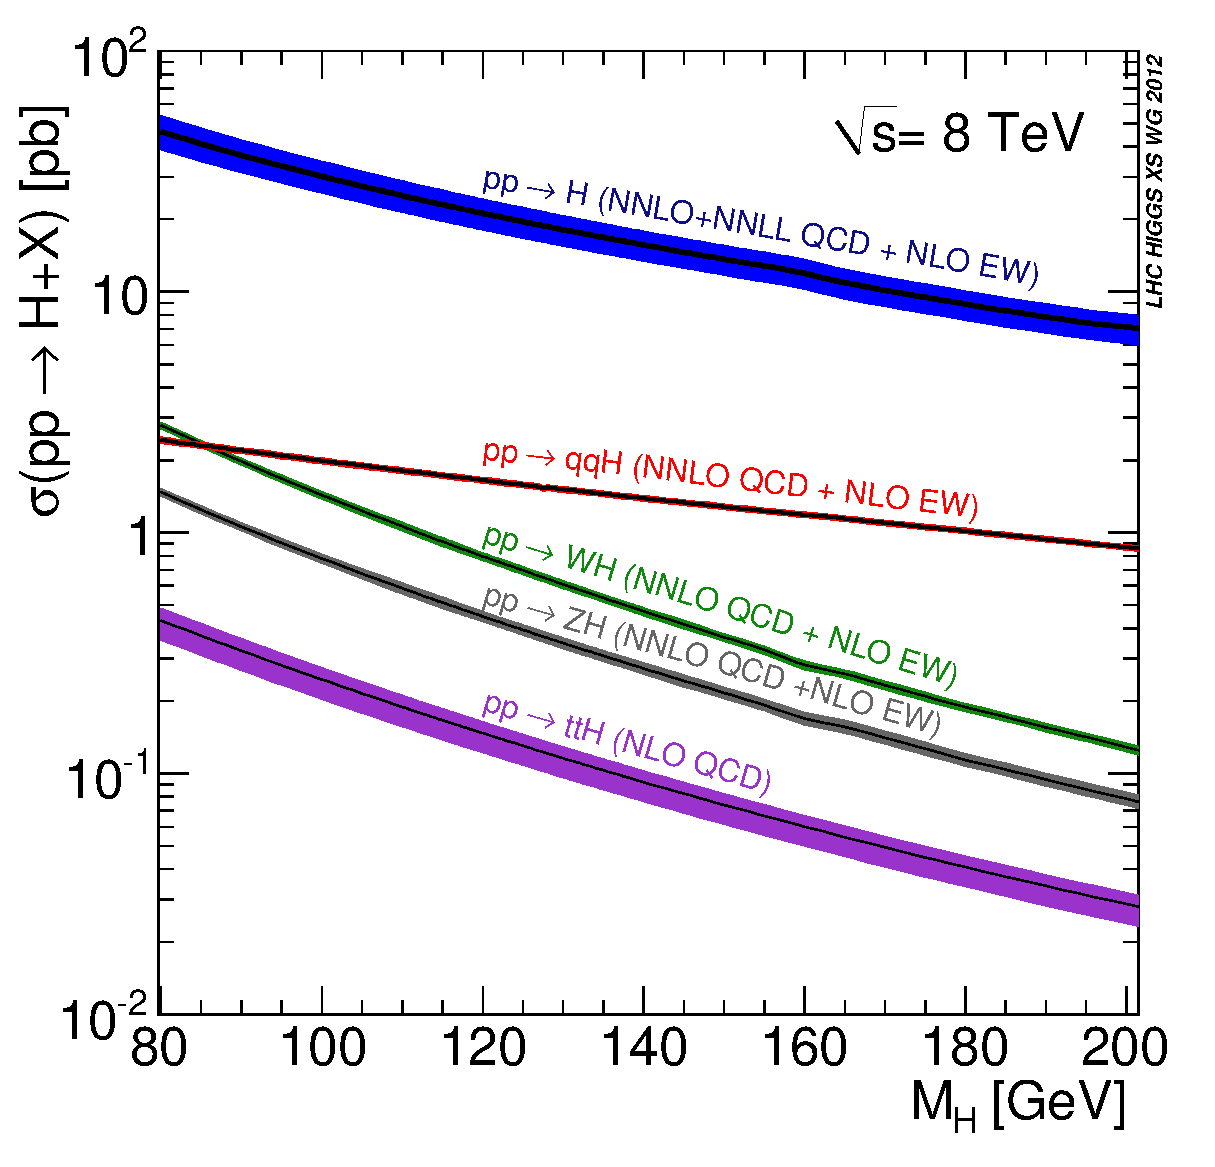
\includegraphics[width=0.8\textwidth]{figures/Higgs_XS_8TeV_LM200.eps}
\caption{ Standard model Higgs production cross sections 
as a function of \mHi{} at $\sqrt{s}=8~\TeV$ for each 
production mode. %\cite{Dittmaier:2012vm}. 
The ggF and VBF processes are 
calculated in complex-pole-scheme (CPS), while other WH/ZH and ttH processes 
are calculated in zero-width-approximation (ZWA). }
\label{fig:Higgs_XS_8TeV_LM200}
\end{figure*}

At hadron collider the hadronic cross section($\sigma$) is calculated with 
parton-level cross-section ($\hat{\sigma}$) convoluted with PDF, 
\begin{eqnarray} 
\sigma (pp \rightarrow H+X) 
= 
\sum_{i,j} \int dx_1 dx_2 f_i(x_1) f_j(x_2) 
\hat{\sigma} \left( ij \rightarrow H+X \right)
\end{eqnarray} 
where i and j are colliding partons, 
$x_1$ and $x_2$ are longitudinal momentum fractions carried by i and j. 
Each component in the equation is subject to the following uncertainties.
The partonic cross section is calculated at given
a renormalizaion scale $\mu_R$ and a factorization scale $\mu_F$. 
Due to possible uncalculated higher-order QCD radiative corrections,
the uncertainty is estimated by varying the scales around 
the central values. In the de Florian and Grazzini (dFG) 
calculation [ref], the central values are chosen to be $\mu_0 = \mHi$. 
The scales $\mu_R$ and $\mu_F$ are varied are in the range 
$\displaystyle \frac{1}{2}\mu_0 < \mu_F, \mu_R < 2\mu_0$ 
with a constraint $\displaystyle \frac{1}{2} < \frac{\mu_F}{\mu_R} < 2$. 
PDF is obtained by fitting on data measured in deep-inelastic scattering, 
Drell-Yan, and jet production from a wide variety of different experiments. 
The accuracy on those data can introduce uncertainty on PDF calculation. 
In addition, strong coupling constant $\alpha_s$ is used in DGLAP evolution [ref] 
to the higher $Q^2$ region. Thus, its uncertainty also contributes to 
the total cross section. There are other uncertainties due to 
the EW corrections, the different choice of top and bottom quark masses, 
and the use of large-$m_T$ method. But, the effect to the 
hadronic cross section is less than a few percent \cite{Dittmaier:2012vm}
for ggF.

Figure \ref{fig:Higgs_XS_8TeV_LM200} shows the hadronic cross sections 
as a function of \mHi{} for SM Higgs production and uncertainty 
in different production modes. The ggF and VBF cross sections 
are based on complex-pole-scheme (CPS), while VH and ttH ones 
are based on zero-width-approximation (ZWA). 
\begin{table}[htb]
\centering
\begin{tabular}{c c c  }
\hline
process     & QCD   & EW \\
\hline \hline 
$ pp \rightarrow H$         & NNLO  & NLO \\
$ pp \rightarrow qqH$       & NNLO  & NLO \\
$ pp \rightarrow WH$        & NNLO  & NLO \\
$ pp \rightarrow ZH$        & NNLO  & NLO \\
$ pp \rightarrow ttH$       & NLO   &     \\
\hline 
\end{tabular}
\label{tab:Higgs_XS_8TeV_order}
\caption{The order of QCD and EW calculations.}
\end{table}
The order of QCD and EW calculations are summarized in Table 
\ref{tab:Higgs_XS_8TeV_order}. The uncertainty is linear combination 
of uncertainties from QCD scale varitaion and PDF+$\alpha_S$.
At $\mHi=125~\GeV$ ggH contributes $\sim 87 \%$ to the total cross section.


%The PDF and parton-level cross section depend on the 
%renormalizaion scale $\mu_R$ because they contain ultraviolet divergences 
%to be subtacted through a renormalization procedure. [ref] 
%In addition PDF is calculated with a factorization scale $\mu_F$.

%%%
\newpage
\subsection{Decay of Higgs Boson}
The interaction term in the Lagrangian shows that the Higgs can 
couple to a pair of weak bosons($VV$). Thus, Higgs decays into $W^+W^-$ and $ZZ$.
Depending on the mass of Higgs, one or two of the bosons can be off-shell. 
Thus we consider three cases where both of them are on-shell$(VV)$, 
one is on-shell and the other is off-shell$(VV^*)$, 
and both of them are off-shell$(V^*V^*)$. 
\begin{itemize} 
%
\item  Both bosons are on-shell($ H \rightarrow VV$) [ref] : 
\begin{eqnarray} 
\Gamma \left( H \rightarrow VV \right) 
= 
\frac{\gf \mHi^3}{16\sqrt{2\pi}} \delta_V \sqrt{1-4\epsilon^2} 
\left( 1 - 4\epsilon^2 - 12\epsilon^4 \right)
\end{eqnarray} 
where $\displaystyle \epsilon = \frac{M_V}{\mHi}$ and $\delta_W=2$ and $\delta_Z=1$.
The ratio of londitudinal polarization is given by \cite{PhysRevD.49.79}
\begin{eqnarray} 
R_L 
= 
\frac{\Gamma_L}{\Gamma_T + \Gamma_L}    
= 
\frac{1 - 4\epsilon^2 - 4\epsilon^4}{1 - 4\epsilon^2 - 12\epsilon^4} 
\xrightarrow{\epsilon \rightarrow 0}{} 1
\end{eqnarray} 
Thus, vector bosons are longitudinally polarized at high \mHi{} ($\epsilon \rightarrow 0$). 
At the production threshold, $\displaystyle \mHi = 2M_V \rightarrow \epsilon = \frac{1}{2}$, 
$R_L$ is 2 which means that longitudinal and transverse polarizations are equally populated. 
In addition, the decay width to WW is reduced to 
\begin{eqnarray} 
\Gamma \left( H \rightarrow WW \right)
&\rightarrow&
\frac{\gf \mHi^3}{16\sqrt{2\pi}} \times 2 \\
&=&  
2 \frac{ 1.16637 \times 10^{-5}~\GeV^{-2} \mHi^3}{16\sqrt{2\pi}} \\
&\approx&
0.33 \mHi \times \frac{\mHi^2}{\TeV^2} (\TeV).   
\end{eqnarray} 
For example, at $\mHi=1~\TeV$, decay width for WW is 0.33 \TeV.
Practically t is hard to claim a Higgs resonance at high mass regions.  
%
\item  one is on-shell and the other is off-shell 
       ($ H \rightarrow VV^* \rightarrow Vf\bar{f}$) where $f$ does not include top quark [ref] : 
\begin{eqnarray} 
\Gamma \left( H \rightarrow VV^* \right) 
=
\frac{3\gf^2 M_v^4}{16\pi^3} \mHi \delta_V' R(\epsilon)
\end{eqnarray} 
where $\delta_W'=1$, $\displaystyle \delta_Z'=\frac{7}{12}-\frac{10}{9}\sin^2\theta_W 
+ \frac{40}{9}\sin^4\theta_W$, and 
\begin{eqnarray}   
\begin{array}{ccc} \multicolumn{2}{c}{\displaystyle 
Rf(\epsilon) = \frac{3(1-8\epsilon^2+20\epsilon^4)}{(4\epsilon^2-1)^{1/2}} 
                \arccos \left( \frac{3\epsilon^2-1}{2\epsilon^3} \right)  
} & \\ & \multicolumn{2}{c}{\hspace{1.5cm} \displaystyle
- (1-\epsilon^2)\left( \frac{47}{2}\epsilon^2 - \frac{13}{2} + \frac{1}{\epsilon^2} \right)  
- 3(1-6\epsilon^2+4\epsilon^4) \ln \epsilon
} \end{array}      
\end{eqnarray} 
\end{itemize} 
The ratio of londitudinal polarization is given \cite{PhysRevD.49.79} by 
\begin{eqnarray} 
R_L 
=
\frac{\Gamma_L}{\Gamma_T + \Gamma_L}    
= 
\frac{R_L(\epsilon)}{R(\epsilon)}  
\end{eqnarray} 
where $R_L$ is \cite{PhysRevD.49.79} 
\begin{eqnarray} 
\begin{array}{ccc} \multicolumn{2}{c}{\displaystyle 
R_L(\epsilon) = \frac{3(1-16\epsilon^2+20\epsilon^4)}{(4\epsilon^2-1)^{1/2}} 
                \arccos \left( \frac{3\epsilon^2-1}{2\epsilon^3} \right)  
} & \\ & \multicolumn{2}{c}{\hspace{1.5cm} \displaystyle
- (1-\epsilon^2)\left( \frac{15}{2}\epsilon^2 - \frac{13}{2} + \frac{1}{\epsilon^2} \right)  
- (3-10\epsilon^2+4\epsilon^4) \ln \epsilon.
} \end{array}      
\end{eqnarray} 

\begin{figure*}[t]
\centering
\includegraphics[width=0.6\textwidth]{figures/HVV_polarization_ratio.pdf}
\caption{The ratio of longitudinal polarization of vector bosons 
as a function of $\frac{\mHi}{2M_V}$ \cite{PhysRevD.49.79} }
\label{fig:HVV_polarization_ratio}
\end{figure*}
Figure \ref{fig:HVV_polarization_ratio} shows the ratio of longitudinally 
polarized vector bosons as a function of $\displaystyle \frac{\mHi}{2M_V}$
(=$\displaystyle \frac{\epsilon}{2}$). 
The ratio changes as \mHi{} changes. Thus, we expect event kinematics differs 
with different \mHi{} hypotheses. This is important when we define signal 
regions optimized at a given \mHi{} hypothesis.  
\textcolor{red}{mention $\Delta\phi_{ll}$ here? What does it mean that 
Vs are transervely polarized? (schemetically)}

\begin{figure*}[t]
\centering
\includegraphics[width=0.45\textwidth]{figures/YRHXS2_BR_Fig1.eps}
\includegraphics[width=0.45\textwidth]{figures/YRHXS_BR_fig2}
\caption{Standard Model Higgs boson decay branching ratios at low \mHi(left) 
and total width (right).}
\label{fig:YRHXS2_BR_Fig1}
\end{figure*}
Figure \ref{fig:YRHXS2_BR_Fig1} shows the branching ratios of Standard 
Model Higgs boson and its total decay width. \textcolor{red}{Top and bottom quarks are 
included in the calculation. Uncertainties are from ...} 

\begin{figure*}[t]
\centering
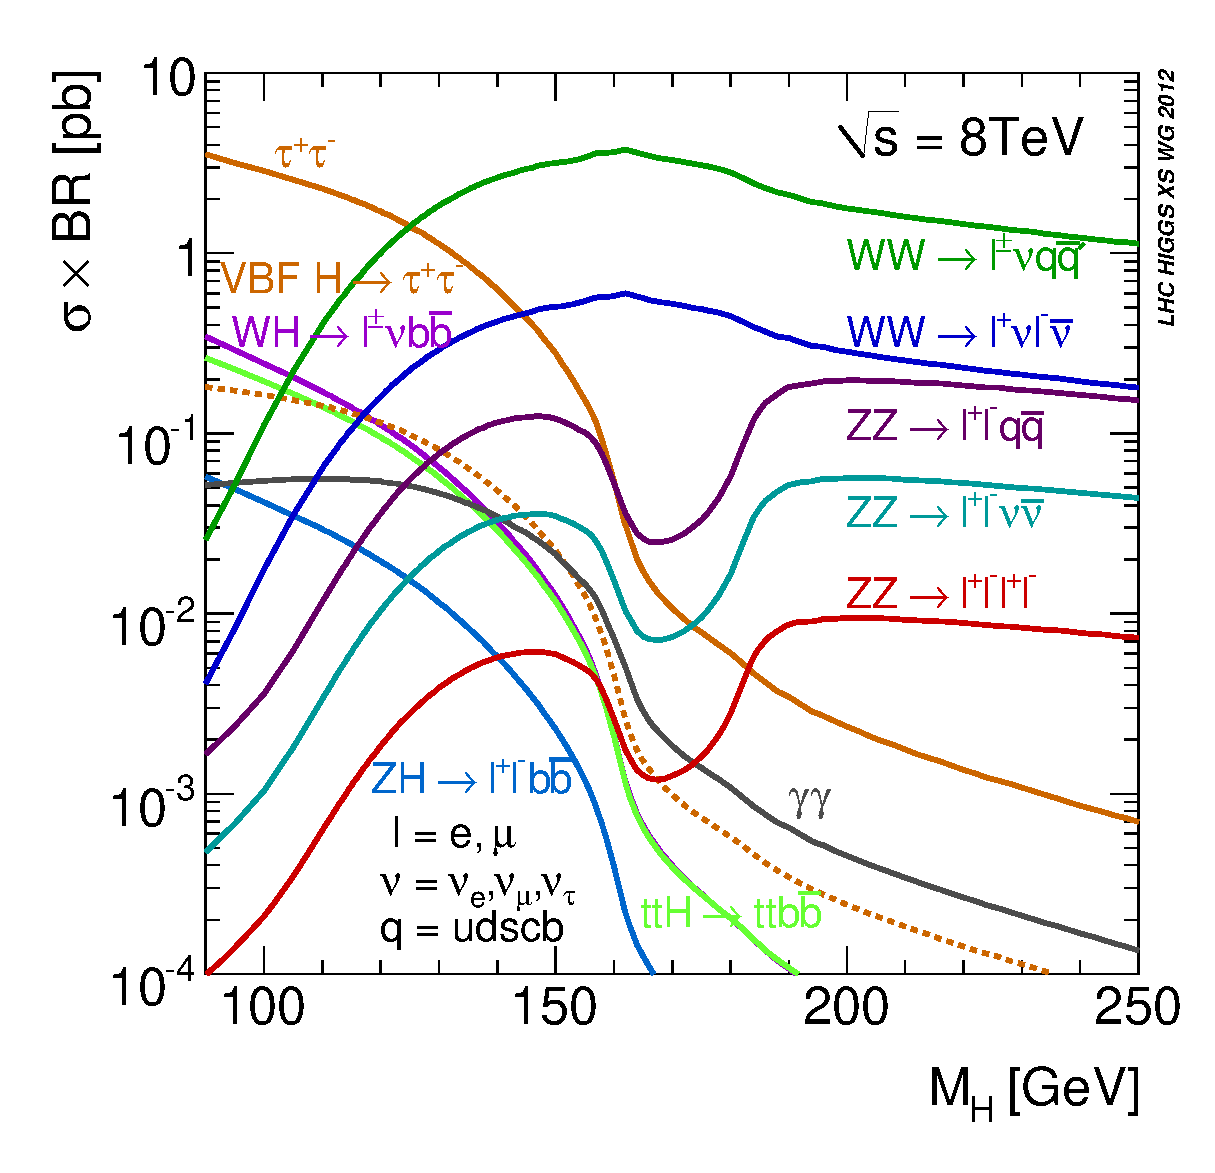
\includegraphics[width=0.6\textwidth]{figures/XSBR_8TeV_SM_LM.eps}
\caption{$\sigma \times BR$ at low \mHi.}
\label{fig:XSBR_8TeV_SM_LM}
\end{figure*}

Figure \ref{fig:XSBR_8TeV_SM_LM} shows $\sigma \times BR$ at low \mHi.


%%%%%%%%%%%%%%%%%%%%%%%%%%%%%%%%%%%%%%%%%%%%%%%%%%%%%%%%%%%%%%%%
\newpage
\section{Limits on Higgs Boson Mass} 

\subsection{Theoretical Limits} 

\subsubsection{Perturbative Unitarity : $W_L^+W_L^- \rightarrow W_L^+W_L^-$}
The cross section of longditudinal vector boson scattering, $V_LV_L \to V_LV_L$, 
increases as the energy increases, which eventually violate unitarity. 
This will be discussed in thie subsection taking  $W_L^+W_L^- \to W_L^+W_L^-$
as an example. 
\begin{figure*}[t]
\centering
\subfigure[]{
\centering
\includegraphics[width=0.25\textwidth]{figures/WWscat0.pdf} 
}
\hspace{0.5cm}
\subfigure[]{
\centering
\includegraphics[width=0.25\textwidth]{figures/WWscat_tchZ.pdf}
}
\hspace{0.5cm}
\subfigure[]{
\centering
\includegraphics[width=0.25\textwidth]{figures/WWscat_schZ.pdf}
}
\\
\vspace{0.5cm}
\subfigure[]{
\centering
\includegraphics[width=0.25\textwidth]{figures/WWscat_tchH.pdf}
}
\hspace{0.5cm}
\subfigure[]{
\centering
\includegraphics[width=0.25\textwidth]{figures/WWscat_schH.pdf}
}
\caption{Feynman diagrams for $W_L^+W_L^- \to W_L^+W_L^-$ scattering.} 
\label{fig:FD_unitary}
\end{figure*}
Fig. \ref{fig:FD_unitary} shows Feynman diagrams for this process.
In the high energy limit $s \gg \mW^2$, the scattering amplitude is \cite{Djouadi20081} 
\begin{eqnarray} 
\label{eq:WWscat}
\mathcal{A}\left( W_L^+W_L^- \to W_L^+W_L^- \right) 
\sim 
- \frac{1}{v^2}  \left( -s - t + \frac{s^2}{s - \mHi^2} + \frac{t^2}{t - \mHi^2} \right). 
\end{eqnarray} 
\textcolor{red}{What does the point diagram correspond to in this equation?}  
According to the Electroweak Equivalence Theorem \cite{31-33} which says 
that at very high energy the longitudinal vector bosons can be replaced by 
their associated Goldstone bosons. Thus, the scattering amplitude can be written 
using Goldstone bosons ($w^\pm$)
\begin{eqnarray} 
\mathcal{A}\left( w^+w^- \to w^+w^- \right) 
= 
- \frac{\mHi^2}{v^2}  \left( 2 + \frac{\mHi^2}{s - \mHi^2} + \frac{\mHi^2}{t - \mHi^2} \right). 
\end{eqnarray} 
An scattering amplitude can be decomposed into partial waves $a_l$
\begin{eqnarray} 
\mathcal{A} = 16 \pi \sum_{i=0}^\infty 
              \left( 2l+1 \right) P_l \left( \cos \theta \right) a_l
\end{eqnarray} 
where $P_l$ is the Legendre polynominals and $\theta$ is the scattering angle.
For $2 \to 2$ cross section using Optical theorem \cite{optical}, we have the 
following identity on cross section ($\sigma$) 
\begin{eqnarray} 
\sigma 
= \frac{16 \pi}{s} \sum_{i=0}^\infty  \left( 2l+1 \right) \left| a_l \right|^2 
= \frac{1}{s} Im \left[ \mathcal{A} \left(\theta = 0 \right)  \right]
\end{eqnarray} 
which gives the unitary condition, 
\begin{eqnarray} 
\left| a_l \right|^2 = Im \left( a_l \right) 
\quad &\Rightarrow& \quad  
Re\left( a_l \right)^2 
+ \left[ Im\left( a_l \right)  - \frac{1}{2} \right]^2 
= \left( \frac{1}{2} \right)^2 \\
\label{eq:unitaryWW}
\quad &\Rightarrow& \quad 
\left| Re \left( a_l \right) \right| < \frac{1}{2}.   
\end{eqnarray} 
Then, the $l=0$ amplitude in the limit of $ s \gg \mHi^2$ becomes  
\begin{eqnarray} 
a_0\left( w^+w^- \to w^+w^- \right)  
&=&  
- \frac{\mHi^2}{16\pi v^2}  
\left[ 2 + \frac{\mHi^2}{s - \mHi^2} 
       - \frac{\mHi^2}{s} \log \left( 1 + \frac{s}{\mHi^2} \right) \right]  \\
&\rightarrow&
- \frac{\mHi^2}{8\pi v^2} 
\end{eqnarray} 
The unitary condition (Eq. (\ref{eq:unitaryWW})) gives upper bound on \mHi, 
\begin{eqnarray} 
\left| Re \left( a_0 \right) \right| 
&=&  \frac{\mHi^2}{8\pi v^2} < \frac{1}{2} \\ 
&\Rightarrow& 
\mHi < 2 \sqrt{\pi} v \simeq 870~\GeV. 
\end{eqnarray} 
Including other scattering channels, 
\begin{eqnarray} 
Z_LZ_L, \,\,\, HH, \,\,\, Z_LH, \,\,\, W_L^+H, \,\,\, W^+_LZ_L 
\end{eqnarray} 
the constraint on \mHi{} becomes tigher \cite{Djouadi20081}, 
\begin{eqnarray} 
\label{eq:unitaryAll}
\mHi < 710~\GeV.
\end{eqnarray}
This means that in SM unitariry will be violated if $\mHi>710~\GeV$
unless there is a new physics that recovers it. 
So far we calculated only tree-level terms, so we can expect that adding 
higher order terms can solve this problem. But, including higher order 
terms does not gaurantee that the unitary will be restored because 
in the high \mHi{} regime coupling to Higgs is too large and perturbative 
calculation breaks down. Thus, the mass bound given in eq.~\ref{eq:unitaryAll}  
can be considered the \mHi~regime where perturbative calculation is reliable 
in all $s$.

\subsubsection{Triviality and Stability bounds}
% Triviality 
\begin{figure*}[t]
\centering
\subfigure[]{
\centering
\includegraphics[width=0.2\textwidth]{figures/FD_HHHHtree.pdf} 
}
\hspace{0.3cm}
\subfigure[]{
\centering
\includegraphics[width=0.2\textwidth]{figures/FD_HHHH1loop1.pdf}
} \hspace{0.3cm}
\subfigure[]{
\centering
\includegraphics[width=0.2\textwidth]{figures/FD_HHHH1loop2.pdf}
}
\hspace{0.3cm}
\subfigure[]{
\centering 
\includegraphics[width=0.2\textwidth]{figures/FD_HHHH1loop3.pdf} } 
\caption{Feynman diagrams for Higgs boson quartic interaction. Left is tree lebel and 
the right three are one-loop correction by Higgs boson itself.} 
\label{fig:FD_triviality} 
\end{figure*} 
The variation of the Higgs quartic couping $\lambda$ is described by Renormalization Group Equation (RGE). 
When we consider one-loop radiation correction by Higgs boson itself to $\lambda$ which are shon in the 
Fig.\ref{fig:FD_triviality}, the corresponding RGE is given by \cite{Djouadi20081} 
\begin{eqnarray} 
\frac{d}{dQ^2} \lambda (Q^2) 
= 
\frac{3}{4\pi^2} \lambda^2(Q^2) + \textrm{higher orders} 
\end{eqnarray} 
The solution to this equation is given by 
\begin{eqnarray} 
\displaystyle  \lambda(Q^2) = \frac{\lambda(v^2)} {\left[\displaystyle   1 - \frac{3}{4\pi^2} \lambda(v^2) \log{\frac{Q^2}{v^2}}\right] } 
\end{eqnarray} 
where the EWSB scale is used as a reference energy point, $Q_0 = v$. 
If the energy is much smaller than the EWSB scale, $Q^2\ll v^2$, 
the quadratic coupling goes to 0, and the theory is called 
``trivial", which means that there is no interaction. 
On the otherhand, if the energy is much larger than the EWSB scale, $Q^2\gg v^2$,
as Q increases the coupling will be infinite at a certain energy scale, $\Lambda_{cut}$. 
Using $\lambda = \mHi^2/2v^2$ and the defition of $\lambda$ that it is positive, 
we have the following equation for denominator,
\begin{eqnarray} 
1 > \frac{3}{4\pi^2} \frac{\mHi^2}{2v^2} \log{\frac{\Lambda_{cut}^2}{v^2}} 
\qquad \Rightarrow  \qquad 
\mHi^2 > \frac{8\pi^2v^2}{\log{\displaystyle  \frac{\Lambda_{cut}^2}{v^2}}},
\end{eqnarray} 
which gives a scale-dependent bound on \mHi. Imposing $\Lambda_{cut} = \mHi$ 
in which case the theory is not reliable, i.e. valid scale of theory is same 
as the mass of a particle, the bound on the Higgs mass is $\mHi < 640~\GeV$. 
This result is consistent with the limit from unitarity constraint. 

% Stability 
In the previous discussion, only was one-loop correction by Higgs itself considered.
This is a proper approximation when $\lambda$ is large. But, in other cases
where $\lambda$ is small, we need to consider the contributions from fermions 
and vector bosons. Since, the strength of interaction with Higgs boson is proportional 
to the particle mass, we consider only heavy particles, vector bosons and top quarks.   
In the limit of small Higgs quartic couplings, $\lambda \ll \lambda_t, g_1, g_2$ 
where $\lambda_t$ is the top Yukawa coupling given by $\sqrt{2} \mt / v$, the RGE is 
given by \cite{Djouadi20081}
\begin{eqnarray}
\label{eq:stability_ddlogQ2}
\frac{d}{dQ^2} \lambda (Q^2)  
\simeq
\frac{1}{16\pi^2}  
\left[ -12 \frac{\mt^4}{v^4} + \frac{3}{16} \left(2g_2^4 + \left(g_2^2+g_1^2\right)^2 \right)   \right].
\end{eqnarray} 
Taking EWSB scale as the reference point, the solution to Eq.~(\ref{eq:stability_ddlogQ2}) is  
\begin{eqnarray} 
\lambda\left(Q^2\right) 
= 
\lambda\left(v^2\right)  
+ 
\frac{1}{16\pi^2}  \left[ -12 \frac{\mt^4}{v^4} 
                          + \frac{3}{16} \left(2g_2^4 + \left(g_2^2+g_1^2\right)^2 \right) \right]
                    \log \frac{Q^2}{v^2}.
\end{eqnarray} 
As $\lambda(v^2)$ becomes small, the couping can go negative, leading the vacuum unstable.   
Thus, in order to maintain the stability of vacuum, $\lambda\left(Q^2\right)$ should be 
positive. This requirement gives
\begin{eqnarray} 
\mHi^2 
&>&
\frac{v^2}{8\pi^2}  \left[ -12 \frac{\mt^4}{v^4} 
                          + \frac{3}{16} \left(2g_2^4 + \left(g_2^2+g_1^2\right)^2 \right) \right]
                    \log \frac{\Lambda_{cut}^2}{v^2} \\
&=&  
\frac{v^2}{8\pi^2}  \left[ -12 \frac{\mt^4}{v^4} 
                          + \frac{3}{16} \left(2g_2^4 + \left(g_2^2+g_1^2\right)^2 \right) \right]
                    \log \frac{\Lambda_{cut}^2}{v^2} \\
&=&  
\textrm{\textcolor{red}{work on this line }}
\end{eqnarray} 
%
\begin{figure*}[t]
\centering
\includegraphics[width=0.8\textwidth]{figures/trivial_vacstab.pdf}
\caption{ Upper and lower bound of \mHi as a function of $\Lambda_{cut}$.
}
\label{fig:trivial_vacstab}
\end{figure*}

So far the higher order contributions were taken up to 1-loop corrections. 
There are calculations upto 2-loops and Fig. \ref{fig:trivial_vacstab} 
shows lower bound (vacuum stability) and upper bound (triviality) of \mHi 
as a function of new cutoff scale, $\Lambda_{cut}$.

%
\subsubsection{Fine tuning}
The 1-loop radiative corrections to Higgs mass when only are W/Z/H and top contributions 
condsidered is given by \cite{Djouadi20081}
\begin{eqnarray} 
\mHi^2 
= 
\left( \mHi^0 \right)^2 + \frac{3 \Lambda_{UV}^2}{8\pi^2v^2} 
\left[ \mHi^2 + 2\mW^2 + \mZ^2- 4 \mt^2 \right] 
\end{eqnarray} 
where $\mHi^0$ is the fundamental parameter of SM and $\Lambda_{UV}$ is the 
UV cutoff scale. Therefore, unless $\Lambda_{UV}$ is in the same scale of 
EWSB($100~\GeV - 1~\TeV$), there should be an incredible fine-tuning between 
$\mHi^0$ and the radiative correction to get \mHi{} in EWSB scale.  
For a quantitative discussion, we first need to define what fine-tuning means. 
Fine-tuning is defined as the sensitivity of the weak scale to
the cutoff, $\left| \delta \mW^2(\Lambda_{UV}) / \mW^2 \right|$, where $\delta \mW^2$ is the 
difference between the tree and loop values, with all other quantities held fixed \cite{Kolda:2000wi}.
So, the metric, $\mathcal{F}$, is  
\begin{eqnarray} 
\mathcal{F}
= \left| \frac{\delta \mW^2}{\mW^2} \right|
= \left| \frac{\delta v^2)}{v^2} \right|
= \left| \frac{\delta \mu^2}{\mu^2} \right|
= \left| \frac{\delta \mHi^2}{\mHi^2} \right|
= \frac{2\Lambda^2}{\mHi^2} \left| \sum_{n} 
  \log^2\left( \frac{\Lambda_{UV}}{\mHi} \right) \right| 
\end{eqnarray} 
and $\mathcal{F} \le 1$ represents that there is no fine-tuning. 
\begin{figure*}[t]
\centering
\includegraphics[width=0.8\textwidth]{figures/finetuning.pdf}
\caption{Constraint contour from fine tuning, vacuum stability, and triviality}.
\label{fig:finetuning}
\end{figure*}
The fig.~\ref{fig:finetuning} \cite{Kolda:2000wi} shows two regions in $[\Lambda,\mHi]$ plane
where $\Lambda$ is the UV cutoff scale, $\Lambda_{UV}$; 
$\mathcal{F}>10$ in light-hatching labeled as $10~\%$ 
and $\mathcal{F}>100$ in thick-hatching labeled as $1~\%$.  
In case of light Higgs scenario, the fine-tuning is even at the low energy scale. 
For example, at \mHi=130 \GeV{} the fineo-tuning of $\mathcal{F}>10(10~\%)$ requires 
$\Lambda<2.3~\TeV$. This means that new physics should exist in the regime where 
LHC experiements can probe.

%%
\newpage
\subsection{Experimental Limits} 

%
\subsubsection{Indirect search} 

There are EWK measurements that are dependent on \mHi. 
\begin{figure*}[t]
\centering
\includegraphics[width=0.3\textwidth]{figures/FD_Wmass_Hloop.pdf}
\caption{Feynman diagram for 1 loop correctioin by Higgs boson to the W propagator.}.
\label{fig:FD_Wmass_Hloop}
\end{figure*}
For example, the mass of W boson has one-loop correction of Higgs boson 
as shown in Fig.~\ref{fig:FD_Wmass_Hloop}. Its contribution to the W mass 
is parametrized by $\Delta r$ in the following equation 
\begin{eqnarray} 
\mW^2 
= 
\frac{\pi\alpha}{\sqrt{2} \gf} 
\frac{1}{\left( 1 - \frac{\mW^2}{\mZ^2} \right)} 
\left( 1 + \Delta r \right),
\end{eqnarray} 
and the correction is 
\begin{eqnarray}
\Delta r \simeq 
\frac{\gf \mW^2}{8 \sqrt{2} \pi^2} \frac{11}{3} 
\left( \log \frac{\mHi^2}{\mW^2} - \frac{5}{6} \right)
\end{eqnarray} 
which is depedent on \mHi{} logarithmically. Thus, by measuring other quantities 
in the equation, we can constrain \mHi{} up to the uncertainties to the measured 
quantities. Going one step further, we can use more variables, not only \mW, 
and put them into a statisitcal fit \cite{LEP-2}. A simultaneous fit is done to
$\Delta \alpha_{had}^{(5)}(\mZ^2)$, $\alpha_S(\mZ^2)$,  
\mZ, \mt, and  $\log_{10} \left( \mHi \right)$
on the data collected by LEP-I/II, SLD, and Tevatron \cite{LEP-2}.  
\begin{figure*}[t]
\centering
%\includegraphics[height=0.4\textheight]{figures/w12_show_higgs.eps}
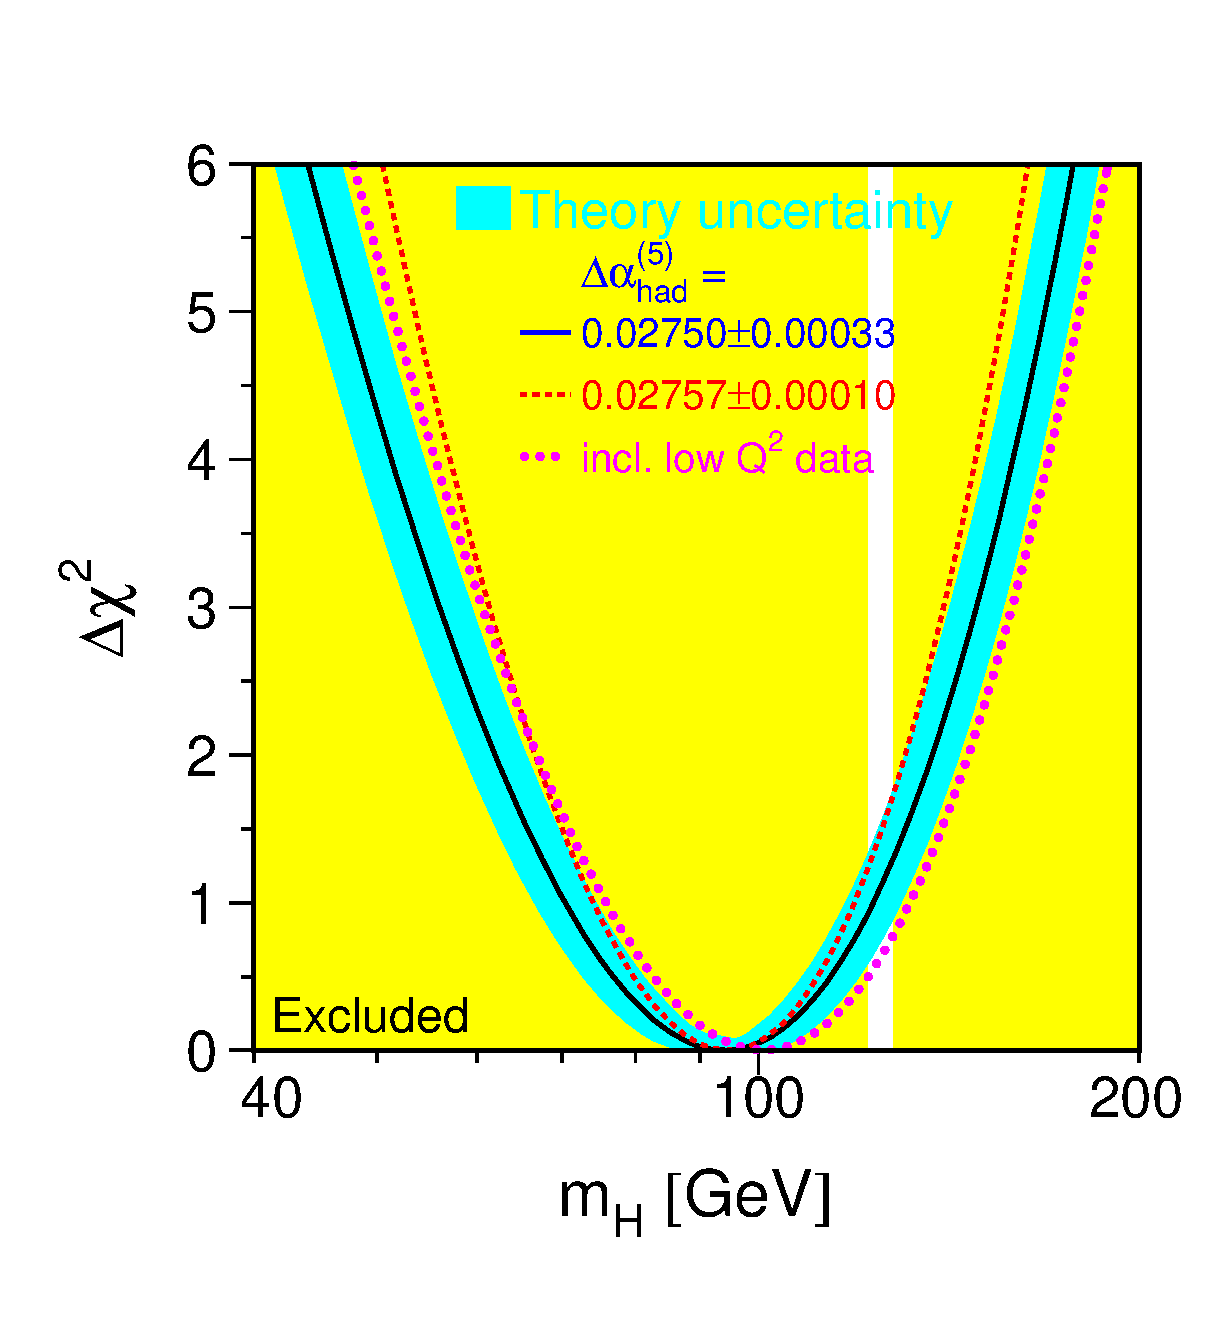
\includegraphics[height=0.5\textheight]{figures/w12_blueband.eps}
\caption{blah}
\label{fig:EWKprecision}
\end{figure*}
The fig.~\ref{fig:EWKprecision} 
%top plots shows the constraints on \mHi %from each variable used by global fit, 
shows $\Delta \chi^2$ curve from EWK precision measurements
assuming that Standard Model is the true theory of nature \cite{LEP-2}. 
The prefered \mHi{} is $94_{-24}^{+29}~\GeV$. It also shows that 
the upper limit on \mHi at C.L. = 95 \% is 152 \GeV. 

%
\subsubsection{Direct search}  

Before 2012, there were direct searches for SM Higgs boson by LEP, Tevatron, 
and LHC experiments. 
The LEP data showed upper limit of $\mHi<114.4~\GeV$ at \CLs = 95 \% \cite{Beringer:1900zz} 
and the Tevatron showed exclusion of SM Higgs hypothesis in the range of 
$147~\GeV < \mHi < 179~\GeV$ at \CLs = 95 \% \cite{Beringer:1900zz}. 
At the end of 2011, the LHC experiments(CMS and ATLAS) showes their 7 TeV results
on the standard model Higgs search \cite{Chatrchyan201226,Aad201249}. 
\begin{figure}[htp]
\centering
\includegraphics[width=0.45\textwidth]{figures/cls_comb_zoom.pdf}
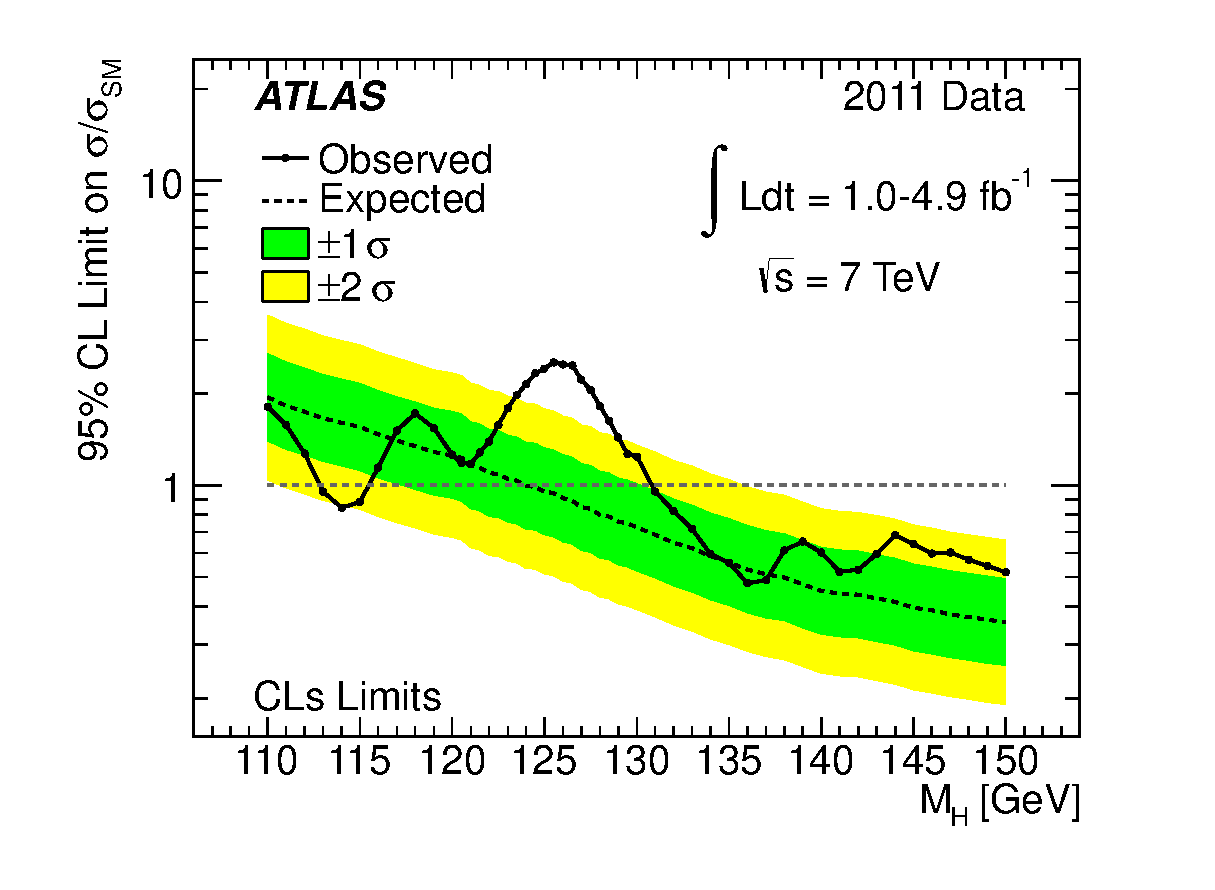
\includegraphics[width=0.45\textwidth]{figures/fig_05b.eps}
\caption{ CMS / ATLAS Higgs exclusion with 7 TeV data. }
\label{fig:2011HiggsExp}
\end{figure}
Fig.~\ref{fig:2011HiggsExp} shows the 95\% C.L. upper limits on $\sigma/\sigma_{\textrm{SM}}$
as a function of \mHi{} in the range of 110 - 145 \GeV{} for CMS on the left and 
110 - 150 \GeV for ATLAS on the right. In both experiments, search was performed up to 
\mHi = 600 \GeV, but only low \mHi{} region is shown on the plots. 
In CMS, the observed exclusion range is 118 - 543 \GeV{} 
with expected exclusion range is 127 - 600 \GeV.     
In ATLAS, the observed exclusion range is 112.9 - 115.5, 131-238, and 251-466 \GeV{} 
with expected exclusion range 124 - 519 \GeV.  
Both experiments, CMS and ATLAS, show local excess of 
$3.1\sigma$ and $3.5\sigma$, repectively, around \mHi = 125 \GeV{} 

 

%%%%
\newpage
\section{\hww} 

%
\subsection{Large expected signal yields}
As seen in the previous section, the $\sigma \times \textrm{BR}$ of \hww{} channel 
is large compared to the other sensitive channels, $H \rightarrow ZZ\rightarrow 4l$
and $H \rightarrow\gamma\gamma$. 
\begin{table}[htb]
\centering
\begin{tabular}{c c c c}
\hline 
        & $H \rightarrow WW \rightarrow 2l2\nu$   & $H \rightarrow ZZ\rightarrow 4l$ 
        & $H \rightarrow\gamma\gamma$  \\
\hline \hline 
$\sigma \times BR (pb)$  
        & $2.24\times10^{-1}$ &  $2.79\times10^{-3}$ & $5.09\times10^{-2}$ \\ 
$N_{expected}$ in $\mathcal{L}_{int} = 20~\ifb$ 
        & 4480 &  56 & 1018 \\ 
\hline 
\end{tabular}
\label{tab:XSBR_8TeV_SM_125}
\caption{$\sigma \times BR$ at $\mHi=125~\GeV$ for most sensitive channels 
and the expected number of events in $\mathcal{L}_{int} = 20~\ifb$.
l means electrons or muons.}
\end{table}
Table \ref{tab:XSBR_8TeV_SM_125} shows $\sigma \times \textrm{BR}$ for 
the most sensitive channels, \hww, $H \rightarrow ZZ\rightarrow 4l$,
and $H \rightarrow\gamma\gamma$ and the expected signal events at
the integrated luminosity, $\mathcal{L}=20~\ifb$. The expected signal 
events are 4480, 56, and 1018, respectively. This allows to have a 
good statistical power to measure the cross section (signal strength)
with this channel. 

%
\subsection{Angular distribution of leptons in the final state}

The spin of SM Higgs is zero, so by helicity conservation the total spin 
of the WW system should be zero. 
\begin{figure}[htp]
\centering
\includegraphics[width=0.7\textwidth]{figures/HiggsSpin.pdf}
\caption{ blah }
\label{fig:HiggsSpin}
\end{figure}
As shown in Fig.~\ref{fig:HiggsSpin}, if we take 
the direction of $W^+$ momentum as z axis in the CM of Higgs,
there are two cases where the spin direction is parellel to the 
momentum direction (transverse polarization) and one case where 
it is perpendicular to the momentum direction(longitudinal polarization). 
In case of transverse polarization, the leptons from Ws have strong 
angular dependence due to V-A nature of weak decays, i.e. neutrinos 
are always left-handed(anti-neutrinos are always right-handed). 
Let's take the case of $W^+$ spin in the z direction as an example.
In order for the neutrino from $W^+$ to be left-handed, the direction 
of the neutrino should be in the - z direction, thus lepton should 
fly to z direction. In order for the anti-neutrino from $W^-$ to be 
right-handed, the direction of the anti-neutrino should be in the 
- z direction, thus lepton should fly to z direction.
Therefore, both leptons tend so move in the same direction 
resulting the angle between the two leptons to be small. 
This is somewhat diluted due to boost of Higgs and Ws, 
but the effect is still visible and used to separate signals 
from non-resonant WW background. 
On the other hand, in case of longitudinal polarization, 
no specific angular correlation is present. 


%
\subsection{Kinematic variables}
\label{subsec:kinimetic_variables}

\begin{figure}[htp]
\centering
\includegraphics[width=0.9\textwidth]{figures/hww_gen_all.pdf}
\caption{ blah }
\label{fig:genhww}
\end{figure}
Figure~\ref{fig:genhww} shows distributions of kinematic variables for 
multiple Higgs hypotheses, $\mHi = 110, 125, 145, 160,\textrm{, and } 200~\GeV$. 
The plotted variables are leading and trailing lepton \pt, 
azimuthal angle difference between the two leptons $\delphill$, 
di-lepton invariant mass $\mll$, and Higgs transverse mass $\mT$ which is 
defined as 
\begin{eqnarray} 
\mT = \sqrt{2\ptll\met(1-cos(\Delta\phi_{\ell\ell-\met}))}
\end{eqnarray} 
where \pt{} is transverse momentum of the dilepton system, 
\met{} is missing transverse momentum, and  
$\Delta\phi_{\ell\ell-\met}$ is the angle between dilepton
direction and \met{} in the transverse plane.
The most of events have leading lepton \ptlmax{} greater than 20~\GeV{} 
for all \mHi{} hypotheses. The The trailing lepton \ptlmin{} is 
quite populated at low \ptlmin{} region, especially for low \mHi{} 
hypotheses. In case of \mHi = 125~\GeV, approximately 25 \% of 
events are rejected by requiring $\ptlmin>10~\GeV$. 
The \delphill, azimuthal angle differece between the two leptons,  
shows non-straightforward trend. The angle tends to get smaller 
as \mHi{} increases up to 160 \GeV, and the angle becomes wide 
after \mHi = 160 \GeV. This behavior was expected in the 
fig.~\ref{fig:HVV_polarization_ratio} where the fraction of the 
longitudinal polarization is at the minimum at \mHi = 2\mW{} which is about 160 \GeV. 
Since small \delphill{} yields small \mll{}, we expect small \mll{} 
for low \mHi hypotheses. The Higgs transverse mass \mT{} shows clear 
drop at \mHi\textcolor{red}{why tail and lazy drop at 200 GeV?}, 

%
\subsection{CMS HWW results as of 2011}

Before 2012, 4.6 \ifb{} of data at $\sqrt{s}=7~\TeV$ collected by CMS detector 
was analyzed for SM Higgs search \cite{Chatrchyan201291}. 
\begin{figure}
\centering
\includegraphics[width=0.9\textwidth]{figures/limits_nj_shape.pdf}
\caption{ Exclusion limit of SM Higgs with 2011 data($\sqrt{s}=7~\TeV$, $\mathcal{L}=4.6~\ifb$ ).
The observed(expected) exclusion limit at CL  = 95 \% is \mHi = 129 - 270(127 - 270) \GeV.}
\label{fig:hww2011}
\end{figure}
Figure~\ref{fig:hww2011} shows exclusion limit using the state-of-the-art 
analysis technique at the time of study. 
The observed exclusion limit at \CLs  = 95 \% is \mHi = 129 - 270 \GeV 
with expected limit \mHi = 127 - 270 \GeV.


%
\chapter{LHC and CMS Detector}
\label{ch:lhc_cms}
%This chapter describes hardware aspects of the Large Hadron Collider(LHC) 
and the Compact Muon Solenoid(CMS) detector. The content is heavily based on 
the chapter 1 of CMS Technical Design Report(TDR) volume 1~\cite{cmstdr1}.


\section{Large Hadron Collider} 

Overview of accelerator, try to answer these questions;   
\begin{itemize}
  \item How beams are focused 
  \item beam crossing angle 
  \item Determination of luminosity and its uncertainty 
\end{itemize}

In order to answer to the key question in the particle physics, 
the origin of mass, physicists constructed a high-energy 
proton-proton(hadrons) collider at CERN. The circumference of the accelator 
is about 27~km, which is large. Thus, the collider is called 
``Large Hadron collider(LHC)". 

The protons are accelerated to the desired collision energy 
going through multiple steps. 
Fig.~\ref{fig:cerncomplex} shows a schematic of the LHC complex. 
The protons are made by applying electric field to hydrogen gas
(Hydrogen atom is composed of one proton and one electron) 
in a metal cylinder. Then, the protons and electrons that constituted 
hydrogen atoms are separated. The separated protons leave 
the metal cylinder at the energy 90~\keV to be 
sent to Radio Frequency Quadrupole(QRF). QRF not only accelerates 
the protons to 750~\keV, but also provides a transverse focusing 
of the beam. The next destination is a linear accelarator(LINAC2) 
where the protons gain energy up to 50~\MeV($v=0.3c$).
The protons are then Proton Synchrotron Booster (PSB) which has 
157~m circumference. The PSB accelerates the protons to 1.4~\GeV\
before sending them to Proton Synchrotron (PS) of 628~m circumference.
PS is responsible for making 81 proton bunches with 25~ns spacing and energy of 25~\GeV($v=0.87c$),  
and send them to Super Proton Synchrotron (SPS) of which circumference is 7~km. 
SPS accelerates the proton bunches to 450~\GeV\ and finally inject them 
to LHC, and they are accelerated to the desired collision energy($v=0.999999c$). 
The lifetime of beams in LHC is around 10 hours and after that 
the protons are dumped to prepare for the next proton fill. 

%
\begin{figure}[ht!] 
\centering 
\includegraphics[width=0.99\textwidth]{figures/Cern-complex.png}
\caption{Schematic of the CERN accelerator complex.} 
\label{fig:cerncomplex} 
\end{figure} 

%Though LHC is a circular accelerator, it is not a perfect circle, 
%but consists of eight 2.45 km arcs and eight 545 m straight insersions. 
%Each arc contains 154 dipole magnets where protons are bent. 

To reach very high collision energy with a fixed size of accelerator, 
the magnetic field that bends the protons should be very high. 
In order to operate at the design proton energy of LHC (7~\TeV), 
the magnetic field should be 8.33~T. This magnetic field is too high, 
LHC uses dipole magnets using electromagnets. For an electronmagnet 
to have a high magnetic field, the current that runs in the rounding coil 
should be high. But, practically this is not easy because the coils will burn 
at high current due to its resistence. LHC dipole magnets use 
niobium-titanium(NbTi) cables with a current 11850~A at the temperature 1.9~K.
The extremely low temperature, 1.9~K, at which the coil becomes a superconductor
is achieved using superfluid helium.  
Fig.~\ref{fig:SCdipole} shows the inner structure, cross section and magnetic field map of
an LHC cryodipole.

%The bunch size of the LHC proton beam 

%
\begin{figure}[ht!] 
\centering 
\includegraphics[width=0.9\textwidth]{figures/cryodipole.jpg} 
\\
\vspace{1cm}
\includegraphics[width=0.45\textwidth]{figures/LHC-PHO-2001-187.jpg}
\includegraphics[width=0.45\textwidth]{figures/LHC-Dipole-Magnetic-Field.png}
\caption{The inner structure, cross section and magnetic field map of
an LHC cryodipole.} 
\label{fig:SCdipole} 
\end{figure} 

The luminosity is given by 
\begin{eqnarray} 
\mathcal{L} = \frac{\gamma f k_B N_p^2}{4 \pi \epsilon_n \beta^*} F 
\end{eqnarray} 
where $\gamma$ is the Lorentz factor, 
$f$ is the revolution frequency, 
$k_B$ is the number of bunches,
$N_p$ is the number of protons per bunch, 
$\epsilon_n$ is the normalized transverse emittance, 
$\beta^*$ the amplitude function at the interaction point, 
and $F$ is the reduction factor due to the crossing angle.
The left figure in fig.~\ref{fig:intlumi} shows the integrated luminosity 
delivered by LHC in 2010, 2011 and 2012 as a function of time each year. 
The delivered intgrated luminosity is 6.1~\ifb\ at $\sqrt{s}=7~\TeV$ in 2011
and 23.3~\ifb\ at $\sqrt{s}=8~\TeV$ in 2012. 

While a perfect detector can record the delivered luminostiy 
with 100~\% efficiency, in reality there are lost collisions 
due data aquisition system being busy and temparary unavailability 
of detector subsystems.  
The right figure in fig.~\ref{fig:intlumi} shows the delivered and the recorded luminosity 
integrated in the 2012 run period. Of the 23.30~\ifb of the delivered luminosity,  
21.79~\ifb is recorded by CMS detector.  

%
\begin{figure}[ht!] 
\centering 
\includegraphics[width=0.45\textwidth]{figures/int_lumi_cumulative_pp_2.pdf}
\includegraphics[width=0.45\textwidth]{figures/int_lumi_per_day_cumulative_pp_2012.pdf}
\caption{Integrated luminosity delivered by LHC in 2010, 2011 and 2012 on left. 
Integrated luminosity delivered by LHC and recored by CMS in 2012 on right.} 
\label{fig:intlumi} 
\end{figure} 

As the proton beams are very squeezed in a proton bunch, there are multiple 
proton-to-proton interactions in one bunch crossing. This multiple interaction 
is called PileUp. The PileUp can be calculated by 
\begin{eqnarray} 
N_\textrm{{PU}} 
= 
\sigma_{\textrm{min bias}} \times \mathcal{L}_{\textrm{bunch crossing}} 
\end{eqnarray} 
where $N_{PU}$ is the number of PileUp events, 
$\sigma_{\textrm{min bias}}$ is the inelastic p-p cross section, 
and $\mathcal{L}_{bunch crossing}$ is the luminosity per bunch crossing.
In 2011 and 2012 the proton bunches crossed every 50~ns 
and the pick instantaneous luminosity is $7.7\times 10^{33} ~\cm^{-2}\textrm{s}^{-1}$. 
Fig.~\ref{fig:pileup2012} shows the PileUp distribution 
of the data recored by CMS detector in 2012 run period. 
The average PileUp is 21. 


%
\begin{figure}[ht!] 
\centering 
\includegraphics[width=0.7\textwidth]{figures/pileup_pp_2012.pdf}
\caption{Number of interactions per bunch crossing in 2012 run period.} 
\label{fig:pileup2012} 
\end{figure} 


\section{Compact Muon Solenoid detector} 

\begin{itemize} 
\item Design concept : target physics process 
\item Coordinate convention : xyz axes, $\phi$, $\eta$, ...
\item Discuss only hardware aspects(purpose of each detector, motivation of design, geometry, specification, electronics, performance ...)
\end{itemize} 

There are two multi-purpose detectors built at the points where 
the two beams collide. Compact Muon Solenoid(CMS) detector~\cite{} is one of them. 
The design of the CMS detector is based on the the detection of SM Higgs boson
in the wide mass range, especially, $H \rightarrow \gamma\gamma$ in the low \mHi\ range 
and $H \rightarrow ZZ \rightarrow 4l$ in the medium \mHi\ range. 
To achieve this the detector need to have good muon identification and momentum resolution, 
good charged particle momeumtum resolution and reconstruction efficiency, 
good electromagnetic energy resolution, and good \met\ and di-jet mass resolution. 
The design of the CMS detector described in the following secions 
is to meet these requirements. 

The momentum and location of physics objects is expressed with respect to the origin 
centered at the collision point in the detector. The x-axis points to the center 
of the collider, the y-axis points upward, and the z-axis goes clock-wise along the 
beam line. CMS uses cylinderical coordinate system due to its cylinderical shape. 
The azimuthal angle, $\phi$, is the angle in the x-y plane 
and the polar angle, $\theta$, is measured with respect to the z-axis. 
Pseudorapidity is defined as $\eta = - \ln \tan(\theta/2)$. 
Advantage of pseudorapidity is that its difference is Lorentz invariant 
under longitidinal boost \footnote[1]{  
In frame O, 
\begin{equation} 
y_1 = \frac{1}{2} \ln \frac{E_1+p_{1L}}{E_1-p_{1L}} \textrm{ and } 
y_2 = \frac{1}{2} \ln \frac{E_2+p_{2L}}{E_2-p_{2L}}  
\end{equation} 
\begin{equation} 
\triangle y = y_1 - y_2 = \frac{1}{2} 
  \ln \frac{(E_1+p_{1L})(E_2-p_{2L})}{(E_1-p_{1L})(E_2+p_{2L})} 
\end{equation} 
In frame O' which is boosted to z direction with velocity $\beta = v / c$, 
\begin{equation} 
\triangle y' = y_1' - y_2' =  \frac{1}{2} 
  \ln \frac{(E_1'+p_{1L}')(E_2'-p_{2L}')}{(E_1'-p_{1L}')(E_2'+p_{2L}')} 
\end{equation}
where 
\begin{equation} 
E_i' = \gamma(E_i - \beta p_i) \textrm{ and } p_i' = \gamma(-\beta E_i + p_i)
\quad \quad \quad \quad (i = 1, 2)
\end{equation} 
Thus we have 
\begin{eqnarray} 
\triangle y' 
 &=& 
 \frac{1}{2} 
  \ln \frac{( \gamma(E_1 - \beta p_{1L})+\gamma(-\beta E_1 + p_{1L})')
            ( \gamma(E_2 - \beta p_{2L})-\gamma(-\beta E_2 + p_{2L}))}
           {( \gamma(E_1 - \beta p_{1L})-\gamma(-\beta E_1 + p_{1L}))
            ( \gamma(E_2 - \beta p_{2L})+\gamma(-\beta E_2 + p_{2L}))}  \\
 &=& 
 \frac{1}{2} 
  \ln \frac{ (E_1+p_{1L})(1-\beta)((E_2-p_{2L})(1+\beta) }
           { (E_1-p_{1L})(1+\beta)((E_2+p_{2L})(1-\beta) } \\ 
 &=& 
 \frac{1}{2} 
  \ln \frac{ (E_1+p_{1L})(E_2-p_{2L}) }
           { (E_1-p_{1L})(E_2+p_{2L}) } \\ 
 &=& \triangle y
\end{eqnarray} 
The rapidity difference is invariant under Lorentz boost along the beam axis. 
}.
Because the initial momentum in z direction is not known due to movement of 
partons inside a proton, and momentum x and y direction is almost zero, 
the momentum and energy of an object is expressed in terms of 
transverse quantitites, \pt\ and $E_T$, calculated in the transverse plane using 
only x and y components.

The overall layout of the CMS detector is as follows. 
Starting from the collision point to outward, there is the inner tracker system(Tracker) 
that is composed of pixel detector and silicon strips and covers $|\eta|<2.5$, 
Electromagnetic calorimeter(ECAL) that covers  $|\eta|<3.0$, 
Hadronic calorimeter(HCAL) that covers  $|\eta|<5.0$, the magnet system, 
and the muon system that covers  $|\eta|<2.4$. 
\textcolor{red}{... make this paragraph richer ... } 
The details of the each sub-detector system are described in the following sections. 



%The design of the CMS detector was driven to achieve good momentum resolution of muons. 
%This requires a strong magnetic field that allows a good momentum measurement 
%of charged particles. Thus, CMS uses superconduncting  


\subsection{Tracker}

The purpose of tracker is to measure momentum of charged particles. 
Based on the charged particle flux, the tracker volume can be divided 
into 3 regions in radial direction. The first region is $r<20~\cm$, closest 
to the interaction vertex. Due to highest particle flux, pixel detectors 
each of which has size of $100 \times 150~\um^2$ are installed. 
The occupancy is about $0.01$ \% per pixel per crossing. 
The second region is $20<r<55~\cm$ and the particle flux is low so that silicon 
microstrip detectors can be used. Minimum size of cell is $10~\cm \times 80~\um$.
The occupancy is about $2-3$ \% per pixel per crossing. 
The third region is $55<r<110~\cm$ and larger-pitch silicon microstrips
are used. The maximum size of a cell is $25~\cm \times 180~\um$.
The occupancy is about $1$ \% per pixel per crossing. 

The layout of the tracker is shown in fig.~\ref{fig:trackerlayout}. 
The total size is 1.1~m in radius and 5.4~m in length. 
In the barrel region, there 3 layers of hybrid pixel detectors
at r = 4.4, 7.3 and 10.2~\cm. The silicon microstrips are 
placed in $20<r<110~\cm$. The barrel region is further separated 
into Inner Barrel(TIB) with 4 layers and Outer Barrel(TOB) with 6 layers. 
In TIB there 3 Inner Disks(TID) in the transition region 
to avoid to small track crossing angle. 
In endcap region, there are 2 pixel and 9 microstrip layers. 
The tracker provides coverage, $|\eta|<2.5$.
%
\begin{figure}[htp] 
\centering 
\begin{tabular}{c} 
\includegraphics[width=0.99\textwidth]{figures/trackerlayout.jpeg} 
\end{tabular} 
\caption{The layout of the CMS tracker~\cite{Anghel2009277}.} 
\label{fig:trackerlayout} 
\end{figure} 

The pixel tracker is composed of 3 layers in barrel and 2 disks in both 
endcap region. The barrel layers are placed at r = 4.4, 7.3 and 10.2~\cm
and each of them has length 53~\cm. The endcap disks cover $6<r<15~\cm$
and located at $|z|=34.5~\cm$ and $46.5~\cm$. The dimension of each 
pixel is $100~\um$ in $r$ and $\phi$, and $150~\um^2$ in $z$.  
The size is chosen to take into account Lorentz drift  
% look at 1.2.1 of http://people.web.psi.ch/kotlinski/CMS/Varia/cmspixel.pdf
\footnote{
Charge carriers in the pixel detector are deflected by the magnetic field perpendicular 
to the electric field. }
and to maintain charge sharing between multiple pixels. 
Each endcap disk is composed of 24 blades assembled to form 
a turbine-like geometry and the blades are rotated by 20~\dg\
considering Lorentz effect. The pixel detector provides 
spatial resolution of 10 and 20~\um\ for $r-\phi$ and $z$ measurements, 
respectively.

The strip tracker is composed of TIB and TOB in barrel region
and TEC and TID in the endcap region. The Number of detectors, thickness,
and mean pitch is shown in the tab.~\ref{tab:silicondetectorspec}.
The first and the second layers of TIB are made with stereo modules
with angle 100~mrad providing single-point resolution of 23-34~\um\
in the $r-\phi$ direction and 230~\um\ in z direction. As TIB, the 
first and the second layers of TOB are made with stereo modules
with angle 100~mrad providing single-point resolution of 35-52~\um\
in the $r-\phi$ direction and 530~\um\ in z direction.
In the endcap region, the first and the second layers of TID, and the first, 
second and the fifth layers of TEC are stereo modules that provide. 
%
\begin{table}[htp] 
\begin{center} 
\small
\begin{tabular}{c|ccccc}  
\hline 
Part & Number of & thickness & mean pitch   & coverage & layers     \\ 
     & detectors & (\um)     & (\um)        &          & (disks)    \\ 
\hline \hline 
%TIB     & 2724  &   320     &   81/118          & $|z|<65~\cm$      & 4     \\ 
%TOB     & 5208  &   500     &   81/183          & $|z|<110~\cm$     & 6     \\ 
%TID     &  816  &   320     &   97/128/143      & $65<|z|<120~\cm$  & 3     \\ 
%TEC     & 2512  &   320     &   96/126/128/143  & $120<|z|<280~\cm$ & 9     \\ 
%TEC(2)  & 3888  &   500     &   143/158/183     &                   &       \\ 
TIB     & 2724  &   320     &   81-118          & $|z|<65~\cm$      & 4     \\ 
TOB     & 5208  &   500     &   81-183          & $|z|<110~\cm$     & 6     \\ 
TID     &  816  &   320     &   97-143          & $65<|z|<120~\cm$  & 3     \\ 
TEC     & 6400  &   320-500 &   96-183          & $120<|z|<280~\cm$ & 9     \\ 
\hline 
\end{tabular} 
\caption{Number of detectors, thickness and mean pitch of each strip, 
coverage in z direction, and number of layers(disks) of the four part of 
silicon strip detector, TIB, TOB, TID and TEC.} 
\label{tab:silicondetectorspec} 
\end{center} 
\end{table} 

Ideal tracker would have no energy loss of charged particles 
while they cross the tracker so that they deposit their initial 
energies in calorimeter. However, real trackers can not be made 
that way due to materials used to build the tracker such as 
electrical cables, cooling servies, support structures, 
electronics and beam-pipe. Fig.~\ref{fig:trackermaterial} shows 
the materal budget of tracker in the units of radiation length($X_0$) 
and interaction length($\lambda_0$). 
%
\begin{figure}[ht!] 
\vspace{1cm}
\centering 
\includegraphics[width=0.99\textwidth]{figures/trackermaterial.jpeg}
\caption{Material budget of CMS tracker in terms of radiation length($X_0$)
and interaction length($\lambda_0$)~\cite{Abbaneo2004331}.} 
\label{fig:trackermaterial} 
\end{figure} 



%%%%%%%%
\subsection{Electromagnetic Calorimeter} 
\begin{itemize}
  \item Selective readout   
  \item Performance  
\end{itemize}

The Electromagnetic Calorimeter(ECAL) is crucial to measure the energy 
of electrons and photons. The CMS ECAL is composed of 61200 and 7324 
lead tunstate($\textrm{PbWO}_4$) scintilating crystals in barrel and 
endcap regions, repectively. $\textrm{PbWO}_4$ crystals have short 
radination length(0.89~\cm) and small Molirere radius(2.2~\cm). 
It is fast in emitting lights and radiation resistant. 
But, it produces relatively low light yields, which requires amplification 
of light signal using photodetectors. Silicon avalanche photodiondes(APD)
are used in barrel and vacuum pohtontriodes(VPT) are used in endcap.
The crystals and APDs are sensitivie with temperature, so the stability
of temperautre is required for operation of ECAL. 

In the barrel region(EB), there are 36 supermodules and each covers 
the region, $0 < |\eta| < 1.479$. 
As shown in fig.~\ref{fig:ecal_EB}, one supermodule contains 4 modules 
and each module has 40 - 50 submodules 
which are composed of 10($2 \times 5$) sub-units(one crystal + one capsule). 
Each crystal covers $0.0174 \times 0.0174$($\approx 1~\dg \times 1~\dg$)
in $\Delta \phi \times \Delta \eta$ and is tilted at 3~\dg\ with respect to the line 
from nominal vertex position. \textcolor{red}{why tilted?}
The length of a crystal is 230~\mm\ which corresponds to $25.8X_0$.
%http://zitogiuseppe.com/oldf/pguide.html

In the endcap region(EE) as shown in fig.~\ref{fig:ecal_EE}, 
the basic unit is supercrystal which is a collection of $5 \times 5$ crystals. 
Each endcap regions is covered 
by two D-shape structred by supercrystals. 
One crystal has the front face size of $28.6 \times 28.6~\mm^2$ 
and length of 220~\mm($24.7X_0$).
Each crystal is off-pointing the nominal vertex as the barrel crystals.  
In the endcap region, the angle between the decayed photons 
is smaller than the barrel region, so an additional deviced is 
needed to distinguish the converted photons from genuine photons.
In order to do this, a preshower device is placed in front of the endcap crystals. 
The preshower device is made of 2 planes of silicon strip detectors with a pitch of 1.9~\mm\
behind disks of lead absorber of depth 2$X_0$ and 3$X_0$.
Due to its finer structure, it provides better spacial resolution 
that enables to reject false photons.  
% preshower : http://cms.web.cern.ch/news/ecal-preshower

%
\begin{figure}[h] 
\vspace{1cm}
\centering 
\begin{tabular}{|c|} 
\hline
\\
\includegraphics[width=0.8\textwidth]{figures/ecal_barrel.jpg} \\
\hline
\end{tabular} 
\caption{Barrel region of ECAL.}
\label{fig:ecal_EB} 
\end{figure} 
%
\begin{figure}[h] 
\vspace{1cm}
\centering 
\begin{tabular}{|c|} 
\hline
\\
\includegraphics[width=0.8\textwidth]{figures/ecal_endcap.jpg} \\
\hline
\end{tabular} 
\caption{Endcap region of ECAL.}
\label{fig:ecal_EE} 
\end{figure} 
%
%\begin{figure}[ht!] 
%\vspace{1cm}
%\centering 
%\includegraphics[width=0.99\textwidth]{figures/EE_Crystal.jpg}
%\caption{Endcap crystal and VPT.}
%\label{fig:EE_crystal} 
%\end{figure} 

The performance of the supermodule in the barrel region is measured 
using a test beam. The electrons in the test beam were indicient on 
the central crystal of $3\times 3$ crystals.
Fig.~\ref{fig:ecal_res} shows its energy resolution($\sigma(E)/E$)
as a function of beam energy(E). The eneryg resolution of calorimeters is 
parametrized by 
\begin{eqnarray}
\left( \frac{\sigma}{E} \right)^2 
= 
\left( \frac{S}{\sqrt{E}}  \right)^2 + \left( \frac{N}{E} \right)^2 + C^2
\end{eqnarray} 
where S is the stochastic term that reflects the fact that the development of showers is    
a statistical process, N is to account for instrumental effects such as noise and pedestals, 
and C is the constant term for calibration errors such as non-uniformitity of detectors.  
The figure shows corresponding values for two curves that use different trigger 
conditions. 

%
\begin{figure}[h] 
\vspace{1cm}
\centering 
\begin{tabular}{|c|} 
\hline
\includegraphics[width=0.6\textwidth]{figures/Figure_001-007.pdf}\\
\hline
\end{tabular} 
\caption{Energy resolution of ECAL supermodule measured using a test beam~\cite{cmstdr1}.}
\label{fig:ecal_res} 
\end{figure} 


%%%%%%%%
\subsection{Hadronic Calorimeter} 

The hadronic calorimeter(HCAL) is made to measure energy of jets.
For the design of HCAL it is important to minimize the Gaussian tails in the energy 
resolution, and to achieve good containment of energy desposit and 
hermeticity for \met\ calculation. CMS HCAL is a sampling detector 
that is composed of alternating layers of an absorber and a scintillator. 
As a hadronic particle hits an absorber plate, interactions occur to produce 
secondary particles, and the these produced particles interact with 
the material in the next layer of absorber, resulting in a shower of 
hadronic particles. When these particles cross the active scintillating  
layers, they cause them to emit lights which can be detected by 
optic devices. The choice of strong magnetic field made most of the 
HCAL built inside of the magnetic coils. This constrained to choose 
a material with short interaction length. For this reason, brass 
is chosen as the HCAL material. The CMS HCAL is organized to 
Hadron Barrel(HB), Hadron Outer(HO), Hadron Endcap(HE) and Hadron Forward(HF).  
Fig.~\ref{fig:hcal_layout} shows the layout of CMS HCAL where HF is not shown. 
%
\begin{figure}[h] 
\vspace{1cm}
\centering 
\begin{tabular}{|c|} 
\hline
\\
\includegraphics[width=0.99\textwidth]{figures/Hcal-segementation-updated.JPG}\\
\hline
\end{tabular} 
\caption{Layout of CMS HCAL~\cite{Chatrchyan:2009hw}.}
\label{fig:hcal_layout} 
\end{figure} 

HB consists of 2304($32 \times 72$ in $\eta \times \phi$) towers of size 
$\Delta \phi \times \Delta \eta = 0.087 \times 0.087$. One HCAL tower 
has the same $\Delta \phi \times \Delta \eta$ coverage as $5\times5$
ECAL crystals. There are 15 brass plates with thickness 5~\cm\ and 
2 stainless steel for mechanical support. The first scintillating 
plate placed before the first brass plate has width of 9~\mm\ while 
the other 16 scintillating plates have width of 3.7~\mm. 

In the barrel, HO which covers $|\eta|<1.26$ is placed to complement 
the short length of HB that may not be enough 
to contain all particles. The escaping showering particles 
is the cause of tail in the energy resolution. Adding HO effectively increases 
the interaction length over 10, thus energy resolution is enhanced.
This is very important for \met\ resolution calculated using calorimeter information. 
HO is divided into 5 sections in $\eta$, resulting 5 rings 
each of which covers 2.5~m in z direction. 
The central ring has two layers of scintillator placed at $r=3.85~\textrm{m}$ and 
$r=4.097~\textrm{m}$ with an iron absorber of thickness 18~\cm\ between them. 
The other rings have one scintillator layer at $r=4.097~\textrm{m}$.

HE is composed of 2304 towers covering $1.3 < |\eta| < 3.0$. 
As shown in left figure of fig.~\ref{fig:hcal_HEHF}, the 5 othermost towers have 
$\phi$ segmentation of 5~\dg\ and $\eta$ segmentation of 0.087. 
The 8 innermost towers have 
$\phi$ segmentation of 10~\dg\ and varying $\eta$ segmentations of 0.09 - 0.35. 

HF is located at $z = \pm 11.2~\textrm{m}$ covering $3.0 < |\eta| < 5.0$. 
It provides improvement in measurement of \met\ 
and reconstruction of forward jets which can be used to identify very interesting 
processes such as Vectro Boson Fusion(VBF)~\cite{}. 
Because HF receive the bulk of particle energy of the collision, 
the material should be resitive to radition. 
HF moduels are made of steel blocks with quartz fibers.
The particles crossing the fibers emit Cherenkov lights 
and the lights are collected by photomultipliers connected to 
the fibers. The right figure of fig.~\ref{fig:hcal_HEHF} shows 
a $\Delta \phi=20~\dg$ wedge of HF.  
The $\phi$ segmentation is 10~\dg\ for all towers except for the 
the two innersmost towers which have $\Delta \phi=$20~\dg. 
The $\eta$ segmentation is 0.175 except for the innermost 
and the outermost towers which have $\Delta \eta=$ 0.3 and 0.1, respectivley. 
%
\begin{figure}[h] 
\vspace{1cm}
\centering 
\begin{tabular}{cc} 
%\hline
\includegraphics[width=0.35\textwidth]{figures/Figure_005-002-a.pdf} & 
\includegraphics[width=0.47\textwidth]{figures/Figure_005-002-b.pdf} \\
%\hline
\end{tabular} 
\caption{Layout of a single wedge of HE(left) and HF(right)~\cite{cmstdr1}.}
\label{fig:hcal_HEHF} 
\end{figure} 

Fig.~\ref{fig:hcal_res} shows resolution of jet transverse energy 
in 3 different $|\eta|$ ranges(0-1.4, 1.4-3.0, 3.0-5.0). 
The resolution is measured using QCD dijet events generated by PYTHIA (version 6.226)
and matching to generator level jet reconstructed stable particles is done by $\Delta R < 0.2$. 
Jets are reconstructed using iterative cone algorithm with a cone size R = 0.5~\cite{}. 
\textcolor{red}{why better resolution in the endcap?}
%
\begin{figure}[h] 
\vspace{1cm}
\centering 
\begin{tabular}{|c|} 
\hline
\includegraphics[width=0.6\textwidth]{figures/Figure_001-008.pdf}\\
\hline
\end{tabular} 
\caption{$E_T$ resolution of jets~\cite{cmstdr1}.}
\label{fig:hcal_res} 
\end{figure} 




%%%%%%%%
\subsection{Magnet} 

The momentum of a charge particle can be determined by measuring 
its curvature in magnetic field. Stronger magnetic field bends   
the trajectory more, thus allows better measurement of momentum.
CMS(as its names indicates) uses superconduncting solenoid 
which produces a uniform magnetic field  3.8(4.0 in design)~T 
in z\textcolor{red}{(or -z ?)} direction.  
The solenoid has 2168 turns and the current to generate 3.8~T magnetic field  
is around 18~kA, giving a stored energy of 2.3~GJ. 
The size of the magnet system is 12.9~m in length and 5.9~m in diameter. 
The three layers of return yokes that guide the magnetic field back to the solenoid 
are installed outside of solenoid, interleaved with the muon system. 
The magnet system also provides mechanical support of the detector
because of its strength and tolerance to its own magnetic field. 
Fig.~\ref{fig:magnet} shows the photos of CMS magnet system : 
return yoke, outer vacuum tank and coil. 

%
\begin{figure}[h] 
\vspace{1cm}
\includegraphics[width=0.99\textwidth]{figures/Figure_CP-1.jpg} \\
\includegraphics[width=0.49\textwidth]{figures/CMS-solenoid-magnet.jpg} 
\includegraphics[width=0.49\textwidth]{figures/magnet-2000-049.jpg}
\caption{Magnet system of CMS~\cite{cmstdr1}. The top photo shows 
the the yoke(red), outer vacuum tank and the coil. The left bottom photon shows 
pictorial view of the magenet system and the right bottom photo shows 
the cross section of coils.}
\label{fig:magnet} 
\end{figure} 



%%%%%%%%
\subsection{Muon System} 

The Muon system of CMS is composed of three gaseous detectors, 
Drift Tube chambers(DT), Cathode Strip Chambers(CSC) and Resistive Plate Chambers(RPC) 
that cover $0<|\eta|<1.2$, $0.9<|\eta|<2.4$ and $0<|\eta|<1.6$, respectively.
Fig.~\ref{fig:muon_system} shows the layout of a quarter of muon system. 
Muon Barrel region(MB) has four layers of muon station interleaved with 
three layers of return yoke. Each layer has a cylinderical shape around 
the beam axis. There are 5 segments in z direction as the return yoke. 
Muon Endcap region(ME) also has four layers(disks) of muon stations
placed perpendicular to the beam axis.
The innermost disk(ME1) has 3 concentric rings and the other disks 
have 2 rings. 
%
\begin{figure}[h] 
\vspace{1cm}
\includegraphics[width=0.99\textwidth]{figures/MuonSys-mod3.png}
\caption{Muon system~\cite{Kim:2012ix}.}
\label{fig:muon_system} 
\end{figure} 

DT chamber consists of 250 chambers constructed in 4 layers at r = 4.0, 4.9, 5.9 
and 7.0~m from the beam axis. Each chamber has 2 superlayers in $\phi$ and 
1 superlayer in z direction. Each superlayer has 4 layers of drift tubes. 
Each drift tube has the width of $\approx$ 4~\cm\ and the height of $\approx$ 1~\cm, 
and there is a streched wire(anode) in the middle of tube filled with a mixture of 
Ar and $\textrm{CO}_2$ gas. When a muon passes through a tube, it knocks 
electrons off the atoms of the gas, and they are drifted to the anode.
Each tube provides 2-dimensional measurement. One is given by the position of 
the central wire, and the other is given by the drift time of electrons divided by
drift speed. Fig.~\ref{fig:muon_dt} shows a schmetic of a 
movement of electrons in a tube and an illustration of a single tube with the
electric field lines. Each station provides $\phi$ precision better than 100~\um\ 
in positin and 1~mrad in direction. 
%
\begin{figure}[h] 
\centering
\vspace{1cm}
\includegraphics[height=0.3\textwidth]{figures/DT.jpg} 
\includegraphics[height=0.3\textwidth]{figures/DT_onetube.jpg}
\caption{Schematic of a superlayer of DT(left) and a tube(right)~\cite{Maselli:1196170}.}
\label{fig:muon_dt} 
\end{figure} 

CSC is composed of 6 gas gaps filled with a mixture of Ar, $\textrm{CO}_2$ and $\textrm{CF}_4$,
and each gap has a plane of radial cathode and a plane of anode wires perpendicular 
tothe strips. The gap between the anode wires is about 3~mm and the width of a strip 
is 3-16~mm. Fig.~\ref{fig:muon_dt} shows a schematic of a CSC on the left 
and an illustration of what happens when a muon passes through a gas gap. 
When a muon tranverses in the gas, it knocks out electrons from the gas atoms. 
Then, an avalanche of electrons is created and moves to the wires.
The ionized positive atoms move toward the strips and make a charge pulse. 
Because the wires are the strips are laid perpendicular to each other, 
each gas gap provides 2-dimensional measurements. 
By weighting by charge distribution, a precise spatial measurements can be made. 
Each CSC provides spatial resolution of 200~\um\ using strips 
and $\phi$ resolution of order of 10~mrad.
Because of fast drift time, CSC is used in the Level-1 trigger. 
%
\begin{figure}[h] 
\centering
\vspace{1cm}
\includegraphics[width=0.99\textwidth]{figures/csc.jpg}
\caption{Schematic of CSC.}
\label{fig:muon_dt} 
\end{figure} 

RPC has one anode plate and one cathode plate organized in parallel
as shown in fig.~\ref{fig:muon_rpc}. 
The plates are separated by a gas chamber of thickness 2~mm 
filled with a mixture of $\textrm{C}_2\textrm{H}_2\textrm{F}_4$ 
and $\textrm{i-C}_2 \textrm{H}_{10}$.
When a muon passes through the chamber, an avalanche of electrons is formed, 
and the electrons are collected by external metallic strips. 
The pattern of the strip hits are then traslated to the momentum measurement
of the muon. Though the spatial resolution of RPC is not as good as DT or CSC,
its time resolution is very good(3~ns), thus it is able to identify 
correct bunch crossing without ambiguities. 
%
\begin{figure}[h] 
\centering
\vspace{1cm}
\includegraphics[width=0.99\textwidth]{figures/rpc.png}
\caption{Schematic of RPC~\cite{Lenzi:2013xpa}.}
\label{fig:muon_rpc} 
\end{figure} 


%%%%%%%%
\subsection{Trigger and Data Acquisition} 
% https://twiki.cern.ch/twiki/bin/view/CMSPublic/WorkBookHLTTutorial

The design bunch crossing rate of 40~Hz yiels $\sim 10^9$ events per second
at the design luminosity. However, only $\sim 100$ Hz of events can be recorded 
on the tape. So, the trigger system should attain about an order of $10^6$ 
reduction of events. CMS trigger and DAQ system is composed of 
detector electronics, Level-1(L1) triggers, readout networks and 
High-Level triggers(HLT). 

The time allocated to L1 trigger decision and data transit is 3.2~\um.
During this time, the data collected by detectors are kept in buffers 
until the decision is made. The decistion is made based on the presence 
of trigger primitives such as photons, electrons, muons and jets 
in the kinematic region of interests. It also employs global sums 
of $E_T$ and \met. Custum hardware processors are used for L1 decision.  
L1 reduces the crossing rate by an order of 1000 targeting 100~kHz.  

Once the L1 decision is made, after further processings, 
the data on the buffer is transferred to the front-end memories for access 
by the DAQ system. The data for an event is sent to a processor 
in a computing farm with $\mathcal{O}(10^3)$ processors. 
Each processor runs the same HLT software to reduce the L1 rate 100~kHz 
down to 100~Hz. The HLT software uses partial event reconstruction, 
and makes decision combining information from multiple virtual trigger 
levels, for example, L2 for calorimeter and muon and L3 for tracking. 
The use of HLT after L1 gives a maximal flexibility because 
it gives freedom in selection. 



%%%%%%%%
\subsection{CMS computing}  
% https://twiki.cern.ch/twiki/bin/view/CMSPublic/WorkBookComputingModel
% https://twiki.cern.ch/twiki/bin/view/CMSPublic/WorkBookCMSSWFramework

Even after the rate of data recording is reduced to 100~Hz by HLT, 
it is still a huge amount of data to store and process. CMS thus employed 
highly distributed computing model(grid system) with Tier-0 center at CERN supplemented 
by Tier-1 and Tier-2 computing centers all around the world. 

Tier-0 center repacks RAW data into primary datasets using trigger information
and send them to Tier-1 centers. It also does prompt reconstruction 
that produces RECO and Analysis Object Data(AOD),
and distribute them to Tier-1. Tier-0 is not accessible by analysers, but  
performs only scheduled activities. 
Tier-1 centers stores a subset of RAW data as backup, provides CPU power for 
re-reconstruction, skimming, calibration and AOD extraction, and 
stores and distributes the produced datasets to Tier-0 or Tier-2. 
Tier-2 centers participate in MC production organized by Tier-1 and 
send the produced MC samples to Tier-1 for distribution in the CMS collaboration. 
Other than this task, Tier-2 serves analysers by providing local computing 
resources as well as grid-based analysis support for the whole experiment.  


%
\chapter{Event Reconstruction and Selection}
\label{ch:event_reconstruction_selection}
%Discuss how basic objects(vertex, electron, muon, jet, MET, top-tagging) 
are reconstructed and what selections are.
Other selections will be discussed in the next chapter, Signal Extraction.

%%%%%%%%%%%%%%%%%%%%%%%%%%%%%%%%%%%%%%%%%%%%%%%%%%%%%%%%%%%%%%%%%%
\section{Trigger}
\label{sec:trigger}
\begin{itemize} 
\item \textcolor{red}{list of triggers} 
\item \textcolor{red}{what are the requirements : already in AN }
\end{itemize} 

As seen in section~\ref{subsec:kinimetic_variables}, \hww{} events have trailing lepton 
whose transverse momentum goes down very low for low \mHi{} hypotheses. Triggering low 
\pt{} leptons is very challenging because of large background events. 
Therefore, in order to record signal events, we need to trigger on the leading lepton, 
or on both leptons. The leading lepton option is not possible because the identification 
and isolation requirements should be very tight and momentum thresholds should be very 
high to maintain sustainable bandwidth. Thus, we trigger on the both leptons. 
The double-lepton triggers we designed for this analysis have high efficiency for  
signal events, but are loose enough to collect events in the several control regions 
we used for various studies. We also use control region triggers that allow 
fake rate and lepton selection efficiency measurements with the precision
good enough for this analysis. 

\textcolor{red}{Where can I check the bandwidth of triggers? want to know 
the total bandwidth of CMS and the bandwidth of triggers we use}

\subsection{Analysis Triggers}

The double-lepton triggers that are listed in Table~\ref{tab:trg_doublelepton} require 
two HLT objects and each of them is required to match an L1 seed. The offline lepton \pt{} 
requirement is 20/10 \GeV, so the online lepton \pt{} reuquirement is a bit looser, 17/8 \GeV, 
in order to be safe from possible tigher online selection. In addition,
the longitudinal distance between the two vertices of the leptons is required 
to be less than 0.2 cm in order to reduce Pile-Up events. 

For electron HLT objects there are additional requirements on
shower shapes, %(H/E, $\sigma_{\eta\eta}$), 
track-to-cluster matching, %($|\Delta\eta|$, $|\Delta\phi|$, $|\frac{1}{E}-\frac{1}{p}|$),
track/calorimeter isolation. %(ECalIso, HCalIso, TrkIso). 
The exact variables and cut values are described in Table~\ref{tab:trg_requirement_def}.
In the table, the naming convention of CMS HLT triggers are shown 
with the corresponding requirements. 
H/E is the ratio of energy deposit in HCAL to that of ECAL. 
$\sigma_{\eta\eta}$ is the weighted sum of \Eta{} difference between the 
seed crystal and the 5x5 crystals surrouding the it.   
$|\Delta\eta|(|\Delta\phi|)$ is the difference in absolute value between 
the center of the supercluster and the direction of the track trajectory 
in \Eta($\phi$) direction.   
$|\frac{1}{E}-\frac{1}{p}|$ is the difference between the reciprocal of supercluster energy 
and the reciprocal of the track momentum.  
$\mathrm{ECalIso/E_T}$, $\mathrm{HCalIso/E_T}$, and $\mathrm{TrkIso/E_T}$ 
are the sum of the trasverse energy within $dR<0.3$ \textcolor{red}{(checked)} 
around the center of energy deposit or track trajectory
divided by the transverse energy, $\mathrm{E_T}$. 
% E_T(SC) for Ecal, and elecand.pt() for Hcal and Tk (guess this is track momentum)  
Because simplified algorithm is used for online variables, the variables 
do not exactly correspond to the offline ones. To account for this, we measure 
tirgger efficiency with respect to the offline selection and do corrections accordingly. 
The details on this can be found in~\ref{subsec:trg_eff} where trigger efficiency 
measurement is discussed.
\textcolor{red}{what is TkMu8? what is the iso requirement on single muon triggers?} 

\begin{table}[!ht]
  \centering 
  \begin{tabular} {l|l}
  \hline
  Double-lepton trigger name & L1 seed \\
  \hline \hline
  HLT\_Ele17\_CaloIdT\_CaloIsoVL\_TrkIdVL\_TrkIsoVL\_ 	    &  L1\_DoubleEG\_13\_7  \\
  Ele8\_CaloIdT\_CaloIsoVL\_TrkIdVL\_TrkIsoVL\_v[15-19] 	&                       \\ 
  %190456-190738 %190762-191419 %191512-194533
  \hline
  HLT\_Mu17\_Mu8\_v[16-22] 	    & L1\_DoubleMu\_10\_Open    \\ %190456-193686 %193806-194533
  HLT\_Mu17\_TkMu8\_v[9-14] 	& OR L1\_DoubleMu\_10\_3p5  \\ %190456-193686 %193806-194533
  \hline
  HLT\_Mu17\_Ele8\_CaloIdT\_CaloIsoVL\_ 	& L1\_Mu12\_EG7     \\
  TrkIdVL\_TrkIsoVL\_v[4-9] 	            &     \\
  %190456-190738 %190762-191419 %191512-193686 %193806-194533
  HLT\_Mu8\_Ele17\_CaloIdT\_CaloIsoVL\_	    & L1\_MuOpen\_EG12       \\ 
  TrkIdVL\_TrkIsoVL\_v[4-9] 	            & OR L1\_Mu3p5\_EG12     \\ 
  %190456-190738 %190762-191419 %191512-193686 %193806-194533
  \hline
  \end{tabular} 
  \caption{Double-lepton triggers used to collect signal events.} 
  \label{tab:trg_doublelepton}
\end{table}
%
\begin{table}[!ht]
  \centering 
  \begin{tabular} {l|l}
  \hline
  Single-lepton trigger name & L1 seed \\
  \hline \hline
  HLT\_Ele27\_WP80\_v[8-11] & L1\_SingleEG20 OR L1\_SingleEG22  \\ 
  %190456-190738 %190762-191419 %191512-194533
  \hline 
  HLT\_IsoMu24\_eta2p1\_v[11-15]   & L1\_SingleMu16er  \\  
  %190456-190738 %190762-193686 %193806-194533
  \hline \hline
  \end{tabular}
  \caption{Single-lepton triggers used to collect signal events.} 
  \label{tab:trg_singlelepton}
\end{table}

%
\begin{table}[!ht]
 \centering
 \begin{tabular}{l|c}
   \hline
   name                       &  criterion \\
   \hline \hline
   \multirow{2}{*}{CaloId\_T} & $\mathrm{H/E < 0.15 (0.10) }$ \\
                               & $\sigma_{\eta\eta}\mathrm{< 0.011\;(0.031)}$ \\
    \hline
   \multirow{2}{*}{CaloId\_VT} & $\mathrm{H/E < 0.05 (0.05) }$ \\
                               & $\sigma_{\eta\eta}\mathrm{< 0.011\;(0.031)}$  \\
    \hline \hline
    \multirow{2}{*}{TrkId\_VL} & $|\Delta\eta|\mathrm{< 0.01\; (0.01)}$ \\
                               & $|\Delta\phi|\mathrm{< 0.15\;(0.10)}$  \\
    \hline
    \multirow{2}{*}{TrkId\_T} & $|\Delta\eta|\mathrm{< 0.008\; (0.008)}$ \\
                              & $|\Delta\phi|\mathrm{< 0.07\;(0.05)}$ \\
    \hline \hline
    \multirow{2}{*}{CaloIso\_VL} & $\mathrm{ECalIso/E_T <0.2\;(0.2)}$ \\
                                 & $\mathrm{HCalIso/E_T <0.2\;(0.2)}$ \\
    \hline
    \multirow{2}{*}{CaloIso\_T} & $\mathrm{ECalIso/E_T <0.15\;(0.075)}$ \\
                                 & $\mathrm{HCalIso/E_T <0.15\;(0.075)}$ \\
    \hline
    \multirow{2}{*}{CaloIso\_VT} & $\mathrm{ECalIso/E_T <0.05\;(0.05)}$ \\
                                 & $\mathrm{HCalIso/E_T <0.05\;(0.05)}$ \\
    \hline \hline
    TrkIso\_VL                   & $\mathrm{TrkIso/E_T <0.2\;(0.2)}$ \\
    \hline
    TrkIso\_T                   & $\mathrm{TrkIso/E_T <0.15\;(0.075)}$ \\
    \hline
    TrkIso\_VT                   & $\mathrm{TrkIso/E_T <0.05\;(0.05)}$ \\
    \hline \hline
    \multirow{8}{*}{WP80} 		& $\mathrm{H/E < 0.10 (0.05) }$ \\
                               	& $\sigma_{\eta\eta}\mathrm{< 0.01\;(0.03)}$ \\
    							& $|\Delta\eta|\mathrm{< 0.007\; (0.007)}$ \\
                               	& $|\Delta\phi|\mathrm{< 0.06\;(0.03)}$  \\
                               	& $|\frac{1}{E}-\frac{1}{p}|\mathrm{< 0.05\;(0.05)}$  \\
    							& $\mathrm{ECalIso/E_T <0.15\;(0.10)}$ \\
                                & $\mathrm{HCalIso/E_T <0.10\;(0.10)}$ \\
                       			& $\mathrm{TrkIso/E_T <0.05\;(0.05)}$\\
    \hline
 \end{tabular}
 \caption{Summary of requirements applied to electrons in the triggers used for this analysis.
The selection requirements are given for electrons in the barrel (endcap).
The abbrevation in the names means L=Loose, VL=Very Loose, T=Tight, and VT=Very Tight.}
 \label{tab:trg_requirement_def}
\end{table}

\subsection{Utility Triggers}

The lepton selection efficiency measurements are performed using \tnp{} method
on \dyll{} events. In order to use \tnp{} method, we should select pure sample 
of \dyll{} events to reduce systematics due to selecting non-prompt leptons from 
other background processes or Pile-Up. Apart from analysis triggers, for this 
kind of study we do not have to select all events, but pure samples with 
adequate statistics. The single lepton triggers used to collect signal events, 
listed in Table~\ref{tab:trg_singlelepton}, can be used to also select 
\dyll{} events. The leading lepton is likely to be triggered, letting the 
trailing leptons be unbiased sample of leptons that covers wide range of 
kinematic region that streches to the low \pt region.   

In order to estimate backgrounds such as \wjets{} that have a non-prompt 
lepton that passes the full lepton selection, we use "fake rate" method.  
The details of this method are discussed in~\ref{sec:wjets}. 
In this method we define a looser selection and calculate the ratio of the 
events that pass the full selection to the events that pass the looser 
selection using single-lepton events dominated by QCD processes. 
The ratio is called fake rate. The fake rate differs by event kinematics
such as \pt{} and \Eta{} of the lepton, and the \pt{} of the leading jet 
that recoils off the lepton. Given that the leptons in the data sample
collected by the analysis triggers are trigger objects, the tighest possible 
loose definition is the trigger requirements of the analysis triggers.
We devised a set of single-lepton triggers that have the looser or same requirements 
on leptons as the double-lepton triggers. Note that the single lepton triggers 
have tighter requirements on leptons. In order to cover large lepton \pt{} range, 
we use several triggers with different lepton \pt{} thresholds.
Because the jet \pt{} distribution is exponentially falling, 
we need triggers that require corrected leading jet \pt{} be greater than 30 \GeV. 
These triggers give sufficient samples for systematic study on fake rate method. 

%For the data-driven estimation for \dyll{} backgrounds we have alternate method 
%that uses photon + jets events. These events are triggered by photon triggers 
%and the photon triggers used for this analysis are listed in the Table~\ref{tab:}.


\begin{table}[!ht]
  \begin{center}
 {\small
  \begin{tabular} {l|l}
\hline
 Trigger name & L1 seed \\
\hline\hline
 HLT\_Ele8\_CaloIdT\_TrkIdVL\_v[2-5]	& L1\_SingleEG5 		\\ %190456-190738 %190762-191419 %191512-194533
 HLT\_Ele8\_CaloIdT\_CaloIsoVL\_		& L1\_SingleEG7 		\\ 
 TrkIdVL\_TrkIsoVL\_v[12-15]			&  						\\ %190456-190738 %190762-191419 %191512-194533
 HLT\_Ele17\_CaloIdT\_CaloIsoVL\_  		& L1\_SingleEG12		\\ 
 TrkIdVL\_TrkIsoVL\_v[3-6]  			& 						\\ %190456-190738 %190762-191419 %191512-194533
 HLT\_Ele8\_CaloIdT\_CaloIsoVL\_      	& L1\_SingleEG7         \\
 TrkIdVL\_TrkIsoVL\_Jet30\_v[3-7]      	& 						\\ %190456-190738 %190762-191419 %191512-194533
 HLT\_Ele17\_CaloIdT\_CaloIsoVL\_		& L1\_SingleEG12		\\ 
 TrkIdVL\_TrkIsoVL\_Jet30\_v[3-7]		& 						\\ %190456-190738 %190762-191419 %191512-194533
	\hline \hline
 HLT\_Mu8\_v[16-18] 	&  L1\_SingleMu3  		\\ %190456 - 194533
 HLT\_Mu17\_v[3-5]      &  L1\_SingleMu12   	\\ %190456 - 194533   
%	\hline \hline
% HLT\_Photon22\_R9Id90\_HE10\_Iso40\_EBOnly\_v[2-4]					& L1\_SingleEG22		\\ %190456-190738 190762-191419 %191512-194731
% HLT\_Photon36\_R9Id90\_HE10\_Iso40\_EBOnly\_v[2-4]					& L1\_SingleEG22		\\ %190456-190738 190762-191419 %191512-194731
% HLT\_Photon50\_R9Id90\_HE10\_Iso40\_EBOnly\_v[2-4]					& L1\_SingleEG22		\\ %190456-190738 190762-191419 %191512-194731
% HLT\_Photon75\_R9Id90\_HE10\_Iso40\_EBOnly\_v[2-4]					& L1\_SingleEG22		\\ %190456-190738 190762-191419 %191512-194731
% HLT\_Photon90\_R9Id90\_HE10\_Iso40\_EBOnly\_v[2-4]					& L1\_SingleEG22		\\ %190456-190738 190762-191419 %191512-194731
    \hline 
  \end{tabular}
}
  \caption{Utility triggers for fake rate method and zeta method. 
  The identification and isolation requirements for electrons are described in Table~\ref{tab:trg_requirement_def}.
%The identification and isolation requirements for photons are described in Table~\ref{tab:PhotonPlusLeptonTriggerCuts}.
}
%and ``$\zeta$ method " are used for Drell-Yan background estimation.}
   \label{tab:triggers_util}
  \end{center}
\end{table}

%
%\begin{table}[htb]
%  \centering
%  \begin{tabular}{l|c}
%    \hline
%    name                        &  criterion \\
%    \hline \hline 
%    \multirow{1}{*}{R9Id90} 	& $\mathrm{R9 > 0.9 }$ \\
%    \hline 
%    \multirow{1}{*}{HE10} 		& $\mathrm{H/E < 0.1 }$ \\
%    \hline 
%    \multirow{3}{*}{Iso40}     	& $\mathrm{ECalIso} < 4.0 $ \\
%                                & $\mathrm{HCalIso} < 4.0 $ \\
%                                & $\mathrm{TrkIso}  < 4.0 $ \\
%    \hline 
%  \end{tabular}
%   \caption{Summary of requirements applied in the photon triggers used for this analysis.}
%   \label{tab:trg_requirement_def_photon}
%\end{table}

%%%%%%%%%%%%%%%%%%%%%%%%%%%%%%%%%%%%%%%%%%%%%%%%%%%%%%%%%%%%%%%%%%
\section{ Event Primary Vertex }
\begin{itemize}
\item \textcolor{red}{Track reconstruction : Kalman Filter, ...}
\item \textcolor{red}{Vertex reconstruction : vertex finding, vertex fitting, ...}
\item \textcolor{red}{Primary Vertex selection}
\end{itemize}

The primary vertices are reconstructed by Deterministic Annealing clustering of 
tracks \cite{davertex}.

The offline primary vertices are required to be within 24 cm from the center of the 
detector\textcolor{red}{(or beamspot?)} in z direction. 
It should be within 2 cm from the beamspot in the radial direction. 
The degrees of freedom of the vertex fit should be 4 or larger. 
\textcolor{red}{what does this mean exactly?} 

At high luminosity collisions, there are multiple proton-proton interactions 
happening at the same bunch crossing. In those interactions there is usually 
only one interaction that is of interest for our analysis, that triggered that event. 
These interactions tend to be associated with energetic objects, 
while the other interactions are mostly inelastic scatterings that produce soft objects.
Therefore, we choose the event primary vertex by selecting the primary vertex 
with largest scalar sum of $\pt^2$ of tracks associated the vertex. 
The vertices of leptons are required to be very close to the event primary vertex.  



%%%%%%%%%%%%%%%%%%%%%%%%%%%%%%%%%%%%%%%%%%%%%%%%%%%%%%%%%%%%%%%%%%
\section{ Electron }
\begin{itemize}
\item \textcolor{red}{Electron reconstruction : GSF track, seeding, ... }
\item \textcolor{red}{ID  : MVA (list of input variables, trainig samples, cut values)}
\item \textcolor{red}{ISO : list of variables to calculate the final cut variable, cut values  }
\end{itemize}

Electrons are reconstructed using tracks and energy deposit ECAL. 
Since they bremsstrahlung in the tracker, this loss of energy should be taken 
into account in the reconstruction. 

An electron candidate is reconstructed if there is a track and a supercluster energy deposit
compatible with the track momentum. When there is a random combination of 
a track from $\pi^\pm$ and a supercluster energy deposit from $\pi^0$ that eventually 
decays to two photons, a fake electron candidate can be made. 
In order to suppress them, we apply electron selection which is composed of 
requirements on identification(track-to-supercluster matching, 
track fit quality, shower shape, energy loss due to bremsstrahlung, ratio of hadronic energy
to electromagnetic energy), isolation, impact parameter.  
Other source of fake electrons is a photon conversion to a pair of electron and a positron 
in the material. If the conversion is asymmetric, \textit{i.e.} one particle carries 
most of the photon momentum, that particle can be selected as an electron 
candidate. Thus, we apply additional requirement on the convertion rejection.

% indentification 
For the electron identification we use BDT-based multivariate approach \cite{electronBDT}.  
The trainig is done with 2011 data; \dyll{} events for signal and QCD-dominated events 
collected by the fakerate triggers listed in section~\ref{sec:trigger}. 
In order to increase the separation by selecting and mitigate possible bias 
due to trigger selections, a set of preselection cuts that are as tight as trigger 
requirements is applied as follows. 
\begin{itemize}
  \item $\pt>10~\GeV$ and $|\eta| < 2.5$
  \item $\sigma_{i\eta i\eta} < 0.01/0.03$ (barrel/endcap)
  \item $|\Delta\phi_{in}| < 0.15/0.10$ (barrel/endcap)
  \item $|\Delta\eta_{in}| < 0.007/0.009$ (barrel/endcap)
  \item $\textrm{H/E}< 0.12/0.10$ (barrel/endcap)
  \item $\displaystyle \frac{\sum_{\textrm{tracks with dR}<0.3}\Et}{\pt}<0.2$
  \item $\displaystyle \frac{\left(\sum_{\textrm{ECAL with dR}<0.3}\Et\right)-1}{\pt}<0.2$
  \item $\displaystyle \frac{\sum_{\textrm{HCAL with dR}<0.3}\Et}{\pt}<0.2$
\end{itemize}
The additional subtraction of 1 GeV in the numerator of ECAL isolation is 
to suppress the constant noise. 
The input variables to the MVA are the following.
\begin{itemize}
\item kinematics : $\pt$,  $\eta$
\item shower shape : $\sigma_{i\eta i\eta}$, $\phi_{i\eta i\eta}$, $\Delta \phi_{SC}$, $\Delta \eta_{SC}$, $E_{3\times3}/E_{5\times5}$(R9), $E_{1\times5}/E_{5\times5}$
\item track fit quality : $\chi^2(\textrm{GSF})/\textrm{ndof} $, $\chi^2(\textrm{CTF})/\textrm{ndof}$ 
\item $\textrm{N}_\textrm{number of tracker layers}$  
\item cluter-track matching (geometry) : $\Delta \phi_{in}$, $\Delta \eta_{in}$, $\Delta \eta_{out}$
\item cluter-track matching (energy-momentum) : $E_{in}/p$, $E/p_{out}$, $1/E_\textrm{ECAL} - 1/p_{\textrm{GSF track}}$ 
\item fraction of energy carried away by bremsstrahlung : $f_{brem}$ 
\item ratio of hadronic energy to EM energy  : $H/E$ 
\item impact parameter :  transverse and 3D impact parameters w.r.t. primary vertex
\item $E_{\textrm{PS}}/E_{\textrm{SC}}$
\end{itemize}
The $\sigma_{i\eta i\eta}$($\phi_{i\eta i\eta}$) is the weighted sum of \Eta($\phi$) 
difference between the seed crystal, \textit{highest energy crystal}, 
and the $5\times5$ crystals surrouding it.
The $\Delta \phi_{SC}$($\Delta \eta_{SC}$) is the width of average distance 
between the seed crystal and the $5\times5$ crystals surrouding it.
The $E_{3\times3}/E_{5\times5}$(R9) and $E_{1\times5}/E_{5\times5}$ 
are the ratio of energy deposit in the $3\times3$($1\times5$) crystals to 
$5\times5$ crystals centered at the seed crystal. 
The $\chi^2(\textrm{GSF})/\textrm{ndof}$ and $\chi^2(\textrm{CTF})/\textrm{ndof}$
are the variables to measure the quality of GSF and CTF track fits, respectively. 
$\textrm{N}_\textrm{number of tracker layers}$ is the number of tracker layers 
where the electron made hits. 
The $\Delta \phi_{in}$($\Delta \eta_{in}$) is the distance in \Eta($\phi$) direction 
between supercluster position and the track trajectory extrapolated from the interaction point
to the SC. $\Delta \eta_{out}$ is the distance in \Eta{} direction
between the supercluster position and the track trajectory extrapolated 
from the supercluster to the interaction point.
$E_{in}/p$ is the ratio of  ... 
$E/p_{out}$ is the ratio of  ... 
$1/E_\textrm{ECAL} - 1/p_{\textrm{GSF track}}$ is the difference between ... 
% Double_t EoP                =   cms2.els_eOverPIn()[ele];
% Double_t eleEoPout          =   cms2.els_eOverPOut()[ele];
% Double_t IoEmIoP            =   1./cms2.els_ecalEnergy()[ele] - 1./cms2.els_p4()[ele].P(); 
The $f_{brem}$ is the ratio of difference between the momemta measured 
at the vertex and the outermost state to the momemtum measured at the 
vertex. This variable shows what franction of the initial momentum  
was lost by bremsstrahlung. 
H/E is the ratio of the energy deposit in the HCAL tower behind the electromagnetic 
seed cluster to the energy of the seed cluster.
$E_{\textrm{PS}}/E_{\textrm{SC}}$ is the ratio of the energy deposit in the preshower 
detector and the energy deposit in the supercluster. 
\begin{table}[!ht]
  \centering 
  \begin{tabular} {c||c|c|c}
  \hline
        & $0<|\eta|<0.8$ & $0.8<|\eta|<1.479$ & $1.479<|\eta|<2.5$\\
  \hline \hline
   $10~\GeV<\pt<20~\GeV$    & 0.0   & 0.1   & 0.62 \\ 
  \hline
   $\pt>20~\GeV$            & 0.94  & 0.85  & 0.92 \\ 
  \hline 
  \end{tabular}
  \caption{Cut values on BDT output for electron identification. Electrons with BDT output
  greater than the corresponding values in the table are considered as good electrons.} 
  \label{tab:electronid_bdtcut}
\end{table}
For selecting good electrons, we finally require the BDT to be greater 
than the values depending on the kinematic region as shown in Table~\ref{tab:electronid_bdtcut}. 

% isolation 
The isolation requirements are imposed by computing isolation variable using 
PF candidates. In the high PileUp environment, there are random contributions 
from ... \textcolor{red}{mention PU issue here}.  
Thus, we need to correct this to mitigate the degradation due to random noise.
To reduce contribution from the random charged PF candidates, they are 
required to be close to the event primary vertex. The contribution from 
the random neutral PF candidates is corrected by subracting the expected contribution. 
The variable is defined as the scalar sum of the \pt{} of the 
PF candidates satisfying the following requirements. 
\begin{itemize}
\item $\Delta R~<~0.4$ to the electron in the $\eta \times \phi$ plane
\item Other PF electrons and PF muons in the isolation cone are vetoed
\item Gamma PF candidates are required to be outside of the footprint 
      veto region of $\Delta R~<~0.08$ 
\item Charged hadron PF candidates are required to be outside of the footprint 
      veto regoin of $\Delta R~<~0.015$ 
\item Charged hadron PF candiates are required to be associated with the event primary vertex
      \textcolor{red}{mention exact value} 
\item Neutral components are corrected by subtracting pileup contribution which is 
      calculated by $\rho \times \textrm{A}_{\rm{eff}}$,
\end{itemize}
where $\rho$ is the event-by-event energy density \cite{} calculated using 
\texttt{kt6PFJets} algorithm, 
and $\textrm{A}_{\textrm{eff}}$ is the effective area shown in Table~\ref{tab:electron_Aeff}. 
\begin{table}[!ht]
  \centering 
  \begin{tabular} {c||c|c|c|c|c|c}
  \hline
    $|\eta|$    & 0 - 1.0 & 1.0 - 1.479 & 1.479 - 2.0 & 2.0 - 2.2 & 2.2 - 2.3 & 2.3 - 2.4  \\
  \hline \hline
    $\textrm{A}_{\rm{eff}}$  & 0.19 & 0.25 & 0.12 & 0.21 & 0.27 & 0.44 \\ 
  \hline 
  \end{tabular}
  \caption{Effective area used for electron isolation calculation.}
  \label{tab:electron_Aeff}
\end{table}
Finally, the isolation variable we cut on is calculated as 
\begin{equation}
\frac{\rm{Iso}_{PF}}{\pt}
=
\left[ \rm{Iso}_{charged \, hadron} + \left\{ \rm{Iso}_{gamma} 
       + \rm{Iso}_{neutral \, hadron} -\rho \times \textrm{A}_{\textrm{eff}} \right\} \right]
\times \frac{1}{\pt}
\end{equation}
where $\rm{Iso}_{charged \, hadron}$, $\rm{Iso}_{gamma}$, and $\rm{Iso}_{neutral \, hadron}$ 
arethe scalar sum of the \pt{} of charged hadron, gamma and neutral hadron PF candidates, 
respectivlely, in the isolation cone of $0.4$ around the electron.
We require $\frac{\rm{Iso}_{PF}}{\pt}$ to be less than $0.15$ in both barrel and endcap.  

% conversion
In order to suppress the electrons from a conversion from a photon, we reject the electron 
if there is a recontructed conversion vertex where one of the two tracks match with 
the electron, if the probability of the conversion vertex fit is greater than $10^{-6}$, 
\verb|What about cms2.convs_dl()[iconv]> dlMin ?|  
and there are any missing hits in the electron track before the conversion vertex.   

% impact parameters
The impact parameter requirements are such that the transverse(longitudinal) impact parameter
between the electron track and the event primary vertex is less than 0.02 cm(0.1 cm). 

The efficiency of the full electron selection measured in MC is \textcolor{red}{XX} \% 
for electrons from HWW 125 and \textcolor{red}{YY} \% for electrons from W+jets.  

%%%%%%%%%%%%%%%%%%%%%%%%%%%%%%%%%%%%%%%%%%%%%%%%%%%%%%%%%%%%%%%%%%
\section{ Muon }
\begin{itemize}
\item \textcolor{red}{Muon reconstruction : ...}
\item \textcolor{red}{ID  : list variables and cut values }
\item \textcolor{red}{ISO : MVA (list of input variables, trainig samples, cut values) }
\end{itemize}

In CMS there are three types of muon reconstruction approaches 
depending on the information(detectors) used in the reconstruction.  

The \textit{Standalone} muon reconstruction uses information from 
the muon system(DT, CSC, RPC), \textit{i.e.} the inner tracker information is not used. 
It starts with the reconstruction of the track segments in the muon chambers. 
The digitized electronic signals in DT, CSC, and RPC are used to 
reconstruct hits. Then, the hits in DT and CSC are matched to form the segments. 
The information of these segments, such as momentum, at the innermost 
muon chamber is used as a seed to construct a muon track using Kalman-filter 
algorithm \cite{kalmanfilter}. The Kalman-filter is an iterative altorithm 
that updates the track parameters iteratively as it goes to the next station. 
At each step of estimating the track parameters, if no matching segment is found 
then the search continues to the next station taking into account the detector 
effects such as multiple scattering and energy loss in the material. 
The procedure goes until the outermost station updating the track parameters 
at each step. After this, the Kalman-filter is applied from the outermost to 
the innermost station, and the track parameters are defined at the innermost 
station. As the last step, the measured muon track is extaploated to the interaction 
point and a vertex-constrained fit is performed to get the final track parameters. 

The \textit{Tracker} muon reconstruction uses information from  
the inner tracker, \textit{i.e.} the muon system information is not used
for the momentum measurement. This approach considers all tracks as 
potential muon candiates and checks their compatibility with 
muon system. All tracker tracks with $\pt>0.5~\GeV$ and $p>2.5~\GeV$ 
are extrapolated to the muon system considering the expected detector effects 
such as magnetic field, multiple scattering, and energy loss in the material. 
If there is at least one muon segment matched to the 
extrapolated track, this muon is considered as the Tracker muon. 
Tracker muon gives good momentum measurement and identification for low \pt{} muons
which is hard to be reconsructed due to leaving not enough track segments 
in the muon system. 

The \textit{Global} muon reconstruction uses information from both tracker 
and the muon system. For a standalone muon track obtained by the way explained 
already, matching between the muon track and a tracker track is performed. 
The muon track at the innermost station is extrapolated to the last layer 
of the tracker considering the expected detector effects 
such as magnetic field, multiple scattering, and energy loss in the material.
Once the matching is done, the Kalman-filter is used to reconstruct the tracks. 
After that, all reconstructed tracks are fitted again without constraints on the 
beamspot using all hits used to reconstruct standalone muons and the hits 
in the silicon strips. A fit is done again using the tracker hits and the 
hits in the innermost muon station, and the fit quality is compared with 
that of the tracker-only fit. This is to detect muon bremsstrahlung  or 
any loss of energy before reaching the muon station.

In summary, there are three approaches for muon reconstruction in CMS. 
Having multiple algorithms provides more reliable muon reconstruction 
and physics analysis can choose their algorithms for their interests. 
\begin{figure}[!hbtp]
\centering
\includegraphics[width=.45\textwidth]{figures/Figure_001-005-a.pdf}
\includegraphics[width=.45\textwidth]{figures/Figure_001-005-b.pdf}
\caption{Resolution of muon momemtun in $0.0<|\eta|<0.2$ and $1.8<|\eta|<2.0$. 
Red, blue, and green are global, standalone, and tracker muons, respectively.} 
\label{fig:muon_res}
\end{figure}
Fig.~\ref{fig:muon_res} shows the momentum resolution of difference muon 
reconstruction algorithms as a function of muon \pt in the barrel(left) and endcap(right). 
The resolution of standalone muons is dominated by mutiple scattering in the material 
before the muon station at $\pt<200~\GeV$ and and by the spacial resolution 
of the muon chambers at $\pt>200~\GeV$. The tracker muons give much better 
resolution at low \pt{}, but the resolution goes up to the same level 
with the stanalone muons at very high \pt. 

The muon selection is composed of requirements on identification, isolation, and 
impact parameters.

%identification
The muon identification requirements are as follows. 
\begin{itemize}
\item The muon should be identified as PF muon 
\item $\pt>10~\GeV$ and $|\eta|<2.4$ 
\item $N_{\textrm{track layers}}>5$ 
\item $N_{\textrm{pixel hits}}$
\item $\displaystyle \frac{\delta \pt}{\pt} < 0.1$  
\item $\displaystyle \frac{\chi^2_{\textrm{kink finder}}}{\textrm{ndof}} < 20$
\item The muon should be global muon or tracker muons  
\end{itemize}
where $N_{\textrm{track layers}}$ is the number of tracker layers where the muon track has hits, 
$N_{\textrm{pixel hits}}$ is the number of pixel hits of the muon track,
$\displaystyle \frac{\delta \pt}{\pt} < 0.1$ is the relative resolution 
of the muon \pt, 
and $\displaystyle \chi^2_{\textrm{kink finder}}/\textrm{ndof}$ is the quality 
of kink finder algorithm which finds muons from decay-in-flights.  
In addtion to these requirements, the muons are required to be the global muons with 
$\chi^2/\textrm{ndof}<10$ on the global fit, 
having at least one muon hit matching the global fit 
\textcolor{red}{(what is the difference between hits and segments?)},  
and having at least two muon segments in different muon stations. 
Or, the muon can be a tracker muon satisfying that at least two muon 
segments one of which is in the outermost muon station are matched.  

%isolation 
For the isolation requirement, the MVA-based isolation variable~\cite{MuonRingIso} is used.
%to reduce contamination from non-isolated muons originating from jets. 
It uses the energy deposits of PF candidates of three categories, 
charged hadron, gamma, and neutral hadrons in the concentric isolation cones
of size $\Delta R = 0-0.1,~0.1-0.2,~0.2-0.3,~0.3-0.4,~0.4-0.5$.
Neutral components are corrected by subtracting Pileup contribution which is 
calculated by $\rho \times \textrm{A}_{\textrm{eff}}$ where $\rho$ (\texttt{kt6PFJets}) is the 
event-by-event energy density and $\textrm{A}_{\textrm{eff}}$ is the effective area.  
Effective areas are from Fall 11 simulation (\texttt{kMuEAFall11MC}) and 
values are shown in Table~\ref{tab:muAeff}.  
Exact definition of input variables to the MVA is the following. 
\begin{itemize}
\item PF charged hadron
	\begin{itemize}
    \item minimum of $\textrm{Iso}_\textrm{PF charged, 01}/\pt$ and 2.5	
    \item minimum of $\textrm{Iso}_\textrm{PF charged, 12}/\pt$ and 2.5	
    \item minimum of $\textrm{Iso}_\textrm{PF charged, 23}/\pt$ and 2.5	
    \item minimum of $\textrm{Iso}_\textrm{PF charged, 34}/\pt$ and 2.5	
    \item minimum of $\textrm{Iso}_\textrm{PF charged, 45}/\pt$ and 2.5	
	\end{itemize}
\item PF gamma : If negative, 0.0 is assigned
	\begin{itemize}
    \item minimum of $\left[\textrm{Iso}_\textrm{PF gamma, 01} - \rho \times \textrm{A}_{\textrm{eff}}\right]/\pt$ and 2.5 
    \item minimum of $\left[\textrm{Iso}_\textrm{PF gamma, 12} - \rho \times \textrm{A}_{\textrm{eff}}\right]/\pt$ and 2.5 
    \item minimum of $\left[\textrm{Iso}_\textrm{PF gamma, 23} - \rho \times \textrm{A}_{\textrm{eff}}\right]/\pt$ and 2.5 
    \item minimum of $\left[\textrm{Iso}_\textrm{PF gamma, 34} - \rho \times \textrm{A}_{\textrm{eff}}\right]/\pt$ and 2.5 
    \item minimum of $\left[\textrm{Iso}_\textrm{PF gamma, 45} - \rho \times \textrm{A}_{\textrm{eff}}\right]/\pt$ and 2.5 
	\end{itemize}
\item PF neutral hadron : If negative, 0.0 is assigned
	\begin{itemize}
    \item minimum of $\left[\textrm{Iso}_\textrm{PF neutral, 01} - \rho \times \textrm{A}_{\textrm{eff}}\right]/\pt$ and 2.5 
    \item minimum of $\left[\textrm{Iso}_\textrm{PF neutral, 12} - \rho \times \textrm{A}_{\textrm{eff}}\right]/\pt$ and 2.5 
    \item minimum of $\left[\textrm{Iso}_\textrm{PF neutral, 23} - \rho \times \textrm{A}_{\textrm{eff}}\right]/\pt$ and 2.5 
    \item minimum of $\left[\textrm{Iso}_\textrm{PF neutral, 34} - \rho \times \textrm{A}_{\textrm{eff}}\right]/\pt$ and 2.5 
    \item minimum of $\left[\textrm{Iso}_\textrm{PF neutral, 45} - \rho \times \textrm{A}_{\textrm{eff}}\right]/\pt$ and 2.5 
	\end{itemize}
\end{itemize}
where we defined 
\begin{eqnarray} 
\textrm{Iso}_\textrm{PF,XY} 
= 
\sum_{
\begin{subarray}{l}
\textrm{PF candidates in the cone of} \\
\textrm{0.X}   < \Delta R^{\mu-\textrm{PF candidate}} < \textrm{0.Y} 
    \end{subarray} }
\pt
%\textrm{the scalar sum of \pt\ of PF candidates in the cone of 0.X} 
%< \Delta R^{\mu-\textrm{PF candidate}} < \textrm{0.Y}.
\end{eqnarray} 
We require that the MVA output be greater than 0.82 (0.86) in $10<\pt~<20~\GeV$ 
and 0.86 (0.82) in $\pt~>20~\GeV$. The cut values correspond to the ones in barrel (endcap).

\begin{table}[htp]
	\centering
		\begin{tabular}{c|c|c|c|c|c|c}
			\hline 
				\multicolumn{7}{c}{PF gamma} \\
	  	    \hline
			 	$|\eta|$     & $0.0 - 1.0$ & $1.0 - 1.479$ & $1.479 - 2.0$ & $2.0 - 2.2$ & $2.2 - 2.3$ & $2.3-$ \\       		
	  	    \hline \hline
				$0.0<dR<0.1$ & 0.004& 0.002& 0.003& 0.009& 0.003& 0.011 \\
				$0.1<dR<0.2$ & 0.012& 0.008& 0.006& 0.012& 0.019& 0.024 \\
				$0.2<dR<0.3$ & 0.026& 0.020& 0.012& 0.022& 0.027& 0.034 \\
				$0.3<dR<0.4$ & 0.042& 0.033& 0.022& 0.036& 0.059& 0.068 \\
				$0.4<dR<0.5$ & 0.060& 0.043& 0.036& 0.055& 0.092& 0.115 \\
	  	    \hline \hline 
				\multicolumn{7}{c}{PF neutral hadron} \\
	  	    \hline 
			 	$|\eta|$     & $0.0 - 1.0$ & $1.0 - 1.479$ & $1.479 - 2.0$ & $2.0 - 2.2$ & $2.2 - 2.3$ & $2.3-$ \\       		
	  	    \hline \hline
				$0.0<dR<0.1$ & 0.002& 0.004& 0.004& 0.004& 0.010& 0.014 \\
			    $0.1<dR<0.2$ & 0.005& 0.007& 0.009& 0.009& 0.015& 0.017 \\
			    $0.2<dR<0.3$ & 0.009& 0.015& 0.016& 0.018& 0.022& 0.026 \\ 
				$0.3<dR<0.4$ & 0.013& 0.021& 0.026& 0.032& 0.037& 0.042 \\ 
				$0.4<dR<0.5$ & 0.017& 0.026& 0.035& 0.046& 0.063& 0.135 \\ 
			\hline
		\end{tabular}
		\caption{ Effective areas used for muon isolation. They were calculated with Fall11 MC sample.}
	\label{tab:muAeff}
\end{table}

%impact parameter 
In addtion, we apply require transverse/longditudinal impact parameters 
to be associated with the event primary vertex. 
The transverse impact parameter is required 
to be less than 0.01 cm for $\pt<20~\GeV$ and 0.02 cm for $\pt>20~\GeV$. 
The longitudinal impact parameter is required to be less than 0.01 cm. 

The efficiency of the full muon selection measured in MC is \textcolor{red}{XX} \% 
for electrons from HWW 125 and \textcolor{red}{YY} \% for electrons from W+jets.  


%%%%%%%%%%%%%%%%%%%%%%%%%%%%%%%%%%%%%%%%%%%%%%%%%%%%%%%%%%%%%%%%%%
\section{ Jet }
\begin{itemize}
\item \textcolor{red}{Jet reconstruction : anti-kT (dR = 0.5) }
\item \textcolor{red}{Jet energy correction : L1Fastjet/L2/L3 (+ Residual correction in data) }
\item \textcolor{red}{lepton veto ($dR>0.3$) }
\item \textcolor{red}{MVA jet ID(list of input variables, training samples, cut values)}
\item \textcolor{red}{two definitions : (1) jet bin counting($\pt>30~\GeV$) (2) top veto($10<\pt<30~\GeV$) }
% have a plot like this for MVA Jet ID? not sure how I drew this though
% maybe a script is somewhere on uaf
%http://uaf-2.t2.ucsd.edu/~jaehyeok/HWW/PhilJetIDMVA/dev/PhilJetIDMVAefssssssss.pdf
\end{itemize}

The existence of gluons and quarks in the event is manifested as a hadronic shower, 
``jets", which leaves an energy deposit primarily in the HCAL. 
Thanks to the fine granuality of CMS detector system, individual hadrons can 
be reconstructed by PF algorithm. 
The, jets are reconstructed with PF candidates using anti-$\textrm{k}_\textrm{T}$ algorithm \cite{}
with a cone size $\Delta R$ = 0.5. Due to the non-linear calorimeter response of CMS detector, 
the measured jet energy can not be translated into the energy of the true parton which 
initiated the jet. CMS employs jet energy correction(JEC) method \cite{} factorized into 
several levels, L1, L2, L3 and residual corrections for data. 
The L1 correction is the PileUp/noise correction, \textit{i.e.} to remove offset energy 
from PileUp and noise. The correction is composed of two sub-correction, 
one from the real jet energy loss due to detector thresholds and 
the other from PileUp. The offset energy in a jet area is measured as a function 
of \Eta{} in the zero-bias and min-bias samples.    
The L2 correction is to make the jet energy response flat in \Eta.  
At a given \Eta{} response is corrected so that the it becomes at the same level 
of the central region, $|\Eta|<1.3$. So, the correction is relative. 
The correction factors are derived from either MC or using data-driven method
(di-jet balance \cite{}).
The L3 correction is to make the jet energy response flat in \pt.  
The central region, $|\Eta|<1.3$, is used as a referece for the correction. 
Apart from the L2 correction, L3 correction is an absolute correction 
such that the corrected jet \pt{} is same as the \pt{} of the parton that 
initiated the jet. The correction factors are derived from either MC 
or using data-driven method($Z/\gamma^*$+jet balance \cite{}). 
For L2 and L3 corrections, the corrections based on MC truth is done for MC 
and residual corrections are applied to data to account for the small differences 
between data and MC. 

Jets fot this analysis are selected first by rejecting overlaps with selected electrons 
and muons. If the $\Delta R$ between a lepton and the jet is less than 0.3, the jet 
is very likely to be a lepton, thus it is rejected. In high PileUp environment, 
clustering random PF particle from PileUp interactions can lead to a high \pt{} jet. 
To suppress this noise, we apply MVA-based PileUp jets suppression techique. 
Jets from pileup are soft, so they need to be overlaid to pass the jet $\pt$ threshold. 
Therefore, energy deposit of pileup jets are more spread than the one from hard interactions.
We select jets of which MVA outputs are greater than the values 
which correspond to the loose working point in Table~\ref{tab:jetidcut}.
\begin{table}[htp]
	\centering
		\begin{tabular}{c|c|c|c|c}
			\hline
									&  $0<|\eta|<2.5$ 	& $2.5<|\eta|<2.75$		& $2.75<|\eta|<3.0$ 	& $3.0<|\eta|<4.7$ 		\\ 
			\hline \hline
				$\pt<10$ \GeV		& 0.0 				& 0.0					& 0.0	 				& 0.2					\\ 
				$10<\pt<20$	\GeV 	& -0.4 				& -0.4					& -0.4	 				& 0.4					\\
				$20<\pt<30$	\GeV	& 0.0 				& 0.0					& 0.2	 				& 0.6					\\ 
				$\pt>30$ \GeV 		& 0.0 				& 0.0					& 0.6	 				& 0.2					\\
			\hline 
		\end{tabular}
		\caption{Cut values on jet identification MVA outputs. MVA output is required to be greater than 
				these values to be counted as a jet.}
	\label{tab:jetidcut}
\end{table}



%%%%%%%%%%%%%%%%%%%%%%%%%%%%%%%%%%%%%%%%%%%%%%%%%%%%%%%%%%%%%%%%%%
\section{ Missing Transverse Energy }
\begin{itemize}
\item \textcolor{red}{How MET(pfMET and trackMET) is calculated } 
\item \textcolor{red}{mention MET $\phi$ modulation correction }
\item \textcolor{red}{define projected MET (compare signal and bkgd, (ex) \ztt)}
\item \textcolor{red}{cut values ($\textrm{minMET} > 20~\GeV$) }
\end{itemize}



%%%%%%%%%%%%%%%%%%%%%%%%%%%%%%%%%%%%%%%%%%%%%%%%%%%%%%%%%%%%%%%%%%
\section{ Top-tagging }
\begin{itemize}
\item \textcolor{red}{How B-tagging algorithm works and working point
      (TCHEM : Track Counting High Efficiency Medium)}
\item \textcolor{red}{how the discriminating variable is calculated }
\item \textcolor{red}{quote some performance plots }
\item \textcolor{red}{soft-muon tagging requirement }
\end{itemize}


%
\chapter{Signal Extraction}
\label{ch:signal_extraction}
%\section{Cut-based Method}
\section{Shape-based Method}


%
\chapter{Efficiency Measurements}
\label{ch:efficiency_measurement}
%%\textcolor{red}{\textbf{!! CAUTION : Efficiency numbers look old. Numbers in AN do not agree with
%/smurf/dlevans/Efficiencies/V00-02-09/HWW\_Electron\_V00-02-09\_Moriond\_V1\_NM1Eff\_ID/summary.txt, 
%but they are from Moriond\_V0. Should replace them. !!}}  


%%%%%%%%%%%%%%%%%%%%%%%%%%%%%%%%%%%%%%%%%%%%%%%%%%%%%%%%%%%%%%%%%%%%%%%%%%%%%%%%%%%%%%%%%%
\section{Lepton Efficiency}

In collisions events are recorded when the two leptons pass trigger requirements. 
Thus, per event trigger efficiency needs to be measured using data. 
To select identified and isolated leptons from Higgs events, we require 
that each lepton meet strict offline criteria. To account for the possible difference
of offline selection efficiencies in simulation and data, we need to measure it 
in simultion and data separately and apply a scale factors
($\epsilon_{data}/\epsilon_{simulation}$) to simulation. 

The efficiencies are measured using Tag-And-Probe method [ref]. We use 
$Z/\gamma^* \rightarrow e^+e^-$ or $Z/\gamma^* \rightarrow \mu^+\mu^-$ events 
passing single-lepton trigger to select unbiased, identified and isolated prompt leptons.  
One lepton which is called "tag" is required to pass the single lepton trigger 
requirement and the full offlince selection. By requiring full selection on the tag, 
we can enhance the purity of the sample. The other lepton which is called 
"probe" is required to pass a set of selection criteria that enhances the purity 
of sample while leaving the crieteria under study unbiased. The fact that tag 
passed sigle-lepton trigger guarantees that the probe is not biased by trigger. 
Both legs can be used as a tag in offline efficiency measurement while only 
can one of them be in trigger efficiency measurement due to the correlation 
between two offlie lepton objects in double-lepton triggers. 

The offline selection efficiency is composed of identification(ID) and isolation(ISO) parts. 
We use N-1 method where ID and ISO efficiencies are measured with respect to the other 
and multiplied afterwards. When measuring efficiency of ID part ($\epsilon_{ID}$) 
probe is required to pass full isolation requirement and when measuring efficiency of 
ISO part ($\epsilon_{ISO}$) probe is required to pass full identification requirement. 
\textcolor{red}{mention that eff is measured as a function of pT and eta of lepton}   
The possible bias due to correlation of the two measurements 
is estimated by comparing efficiencies measured by N-1 method and combined measurement 
of ID+ISO  efficiency in simulation. The difference which ranges from xx to yy depending 
on the kinemtic bins of a lepton is assigned as systematic uncertainty of the method. 
\textcolor{red}{What are the other systematics? For electron, systematics to 
electron reconstruction efficiency(prob for a SC to be matched to a ECAL-driven 
GSF electron), 100 +/- 2\% (measured with 2011 data). In the code, there are 
2 \% and 1.5 \% for electron and muon, repectively. Are they from 
reconstruction efficiency and other ones are negligible compared to these values?} 

Requiring tight selections to tag and using N-1 method gives high-purity sample 
of $Z/\gamma^*$ events in data. However, there are residual contributions from 
non-prompt leptons from W+jets and QCD events especially at low $p_T$ bins. 
Thus, we extract yields by fitting the \mll~distribution of the tag and probe pair
with Gaussian $+$ exponential $\times$ error function. The Gaussian function which 
is for $Z/\gamma^*$ invariant mass peak is modeled by simulation and 
gaussian smearing is applied to account for difference in lepton momentum resolutions
between data and simulation. 
\textcolor{red}{I don't believe this is true. Looking at the plots with fitted shapes, 
it seems that there are more than one fit function. need to check in the code.}
The exponential $\times$ error function is for backgrounds.
To allow enough sidebands for backgrounds, \mll~range is chosen to be 
$60~\GeV < \mll < 120~\GeV$. In case of simulation, efficiencies are calculated by 
counting events in $81~\GeV < \mll < 101~\GeV$. In simulation, to select  
leptons from $Z/\gamma^*$ only (=to remove mis-recontructed leptons), the dR between 
probe and the closest, same flavor, generator-level lepton after final-state-radiation(FSR)
is required to be within 0.2.

The data/simulation efficiency scale factors per event are then calculated by 
multiplying per lepton efficiencies measured in data and simulation, 
\begin{equation} 
\epsilon_{offline}^{event} 
= 
\epsilon_{ID}^{lepton1} \times \epsilon_{ISO}^{lepton1}   
\times \epsilon_{ID}^{lepton2} \times \epsilon_{ISO}^{lepton2}.   
\end{equation} 
The trigger efficiency($\epsilon_{trigger}$) is measured with respect to the full 
offline selection. Finally, simulation events are corrected by applying the 
offline selection scale factor and trigger efficiency, 
\begin{equation} 
\frac{\epsilon_{offline, MC}^{event}}{\epsilon_{offline, MC}^{event}} 
\times \epsilon_{trigger}. 
\end{equation} 



%%%%%%%%%%
\subsection{Electron Selection Efficiency}

Electron efficiency is composed of two factors, recontruction efficiency and 
selection efficiency. The reconstruction efficiency is the probability for a 
super-cluster energy deposit to be matched to a reconstructed ECAL-driven 
GSF electron. For thie analysis, we use the result measured with 2011 data   
because new measurement has not made with the full 2012 data sample[ref]. 
\textcolor{red}{Really no new study?}. The efficency is measured as a function 
of \pt~and \Eta~of a lepton. From the study, we assume that the reconstruction 
efficiency for an electron is unity with uncertainty at the level of 2 \%.

%
\begin{table}[!htp]
\begin{center}
\begin{tabular}{c|c|c|c|c}
\hline & $ 0 < |\eta| < 0.8$ & $ 0.8 < |\eta| < 1.479$ & $ 1.479 < |\eta| < 2 $ & $ 2 < |\eta| < 2.5 $  \\
\hline
\multicolumn{5}{c} {N-1 Efficiencies in data} \\
\hline
$ 10 < p_T <  15$ & $0.3289 \pm 0.0049$ & $0.4353 \pm 0.0046$ & $0.1551 \pm 0.0040$ & $0.1059 \pm 0.0026$  \\
$ 15 < p_T <  20$ & $0.5981 \pm 0.0026$ & $0.6330 \pm 0.0028$ & $0.3140 \pm 0.0033$ & $0.2379 \pm 0.0030$  \\
$ 20 < p_T <  30$ & $0.7208 \pm 0.0009$ & $0.7457 \pm 0.0010$ & $0.5147 \pm 0.0011$ & $0.4609 \pm 0.0021$  \\
$ 30 < p_T <  40$ & $0.8293 \pm 0.0002$ & $0.8481 \pm 0.0004$ & $0.6780 \pm 0.0015$ & $0.5962 \pm 0.0015$  \\
$ 40 < p_T <  50$ & $0.8623 \pm 0.0004$ & $0.8840 \pm 0.0005$ & $0.7558 \pm 0.0007$ & $0.6573 \pm 0.0009$  \\
$ 50 < p_T < 7000$ & $0.8745 \pm 0.0004$ & $0.8936 \pm 0.0005$ & $0.7859 \pm 0.0012$ & $0.6891 \pm 0.0015$  \\
\hline
\multicolumn{5}{c} {N-1 Efficiencies in simulation} \\
\hline
$ 10 < p_T <  15$ & $0.4583 \pm 0.0055$ & $0.5405 \pm 0.0053$ & $0.2267 \pm 0.0058$ & $0.1890 \pm 0.0056$  \\
$ 15 < p_T <  20$ & $0.6671 \pm 0.0030$ & $0.7126 \pm 0.0031$ & $0.3904 \pm 0.0045$ & $0.3426 \pm 0.0047$  \\
$ 20 < p_T <  30$ & $0.7594 \pm 0.0010$ & $0.7943 \pm 0.0011$ & $0.5762 \pm 0.0019$ & $0.5090 \pm 0.0021$  \\
$ 30 < p_T <  40$ & $0.8492 \pm 0.0005$ & $0.8797 \pm 0.0005$ & $0.7215 \pm 0.0010$ & $0.6291 \pm 0.0012$  \\
$ 40 < p_T <  50$ & $0.8774 \pm 0.0004$ & $0.9091 \pm 0.0004$ & $0.7843 \pm 0.0007$ & $0.6915 \pm 0.0010$  \\
$ 50 < p_T < 7000$ & $0.8893 \pm 0.0007$ & $0.9169 \pm 0.0007$ & $0.8039 \pm 0.0013$ & $0.7149 \pm 0.0017$  \\
\hline
\multicolumn{5}{c} {Simulation-to-data scale factors} \\
\hline
$ 10 < p_T <  15$ & $0.7177 \pm 0.0138$ & $0.8053 \pm 0.0117$ & $0.6842 \pm 0.0249$ & $0.5602 \pm 0.0214$  \\
$ 15 < p_T <  20$ & $0.8966 \pm 0.0056$ & $0.8882 \pm 0.0055$ & $0.8045 \pm 0.0126$ & $0.6943 \pm 0.0128$  \\
$ 20 < p_T <  30$ & $0.9491 \pm 0.0017$ & $0.9388 \pm 0.0019$ & $0.8933 \pm 0.0035$ & $0.9056 \pm 0.0056$  \\
$ 30 < p_T <  40$ & $0.9766 \pm 0.0006$ & $0.9641 \pm 0.0007$ & $0.9396 \pm 0.0024$ & $0.9477 \pm 0.0030$  \\
$ 40 < p_T <  50$ & $0.9828 \pm 0.0006$ & $0.9724 \pm 0.0007$ & $0.9637 \pm 0.0013$ & $0.9507 \pm 0.0018$  \\
$ 50 < p_T < 7000$ & $0.9834 \pm 0.0009$ & $0.9746 \pm 0.0009$ & $0.9776 \pm 0.0021$ & $0.9639 \pm 0.0032$  \\
\end{tabular}
\caption{HWW Electron V00-02-09 Moriond jae NM1Eff ID}
\label{tab:eff_electron_id}
\end{center}
\end{table}

\begin{table}[!htp]
\begin{center}
\begin{tabular}{c|c|c|c|c}
\hline & $ 0 < |\eta| < 0.8$ & $ 0.8 < |\eta| < 1.479$ & $ 1.479 < |\eta| < 2 $ & $ 2 < |\eta| < 2.5 $  \\
\hline
\multicolumn{5}{c} {N-1 Efficiencies in data} \\
\hline
$ 10 < p_T <  15$ & $0.7827 \pm 0.0042$ & $0.7973 \pm 0.0029$ & $0.8009 \pm 0.0199$ & $0.8546 \pm 0.0110$  \\
$ 15 < p_T <  20$ & $0.8167 \pm 0.0007$ & $0.8360 \pm 0.0034$ & $0.8155 \pm 0.0145$ & $0.8776 \pm 0.0041$  \\
$ 20 < p_T <  30$ & $0.8798 \pm 0.0011$ & $0.8815 \pm 0.0007$ & $0.8787 \pm 0.0017$ & $0.9246 \pm 0.0091$  \\
$ 30 < p_T <  40$ & $0.9391 \pm 0.0000$ & $0.9398 \pm 0.0007$ & $0.9337 \pm 0.0006$ & $0.9598 \pm 0.0004$  \\
$ 40 < p_T <  50$ & $0.9710 \pm 0.0001$ & $0.9721 \pm 0.0002$ & $0.9704 \pm 0.0002$ & $0.9802 \pm 0.0002$  \\
$ 50 < p_T < 7000$ & $0.9816 \pm 0.0002$ & $0.9815 \pm 0.0008$ & $0.9815 \pm 0.0003$ & $0.9873 \pm 0.0004$  \\
\hline
\multicolumn{5}{c} {N-1 Efficiencies in simulation} \\
\hline
$ 10 < p_T <  15$ & $0.7724 \pm 0.0061$ & $0.8015 \pm 0.0052$ & $0.7856 \pm 0.0109$ & $0.8516 \pm 0.0110$  \\
$ 15 < p_T <  20$ & $0.8214 \pm 0.0027$ & $0.8362 \pm 0.0028$ & $0.8213 \pm 0.0052$ & $0.8761 \pm 0.0053$  \\
$ 20 < p_T <  30$ & $0.8850 \pm 0.0008$ & $0.8906 \pm 0.0009$ & $0.8768 \pm 0.0016$ & $0.9091 \pm 0.0017$  \\
$ 30 < p_T <  40$ & $0.9464 \pm 0.0003$ & $0.9473 \pm 0.0003$ & $0.9360 \pm 0.0006$ & $0.9484 \pm 0.0007$  \\
$ 40 < p_T <  50$ & $0.9757 \pm 0.0002$ & $0.9768 \pm 0.0002$ & $0.9708 \pm 0.0003$ & $0.9720 \pm 0.0004$  \\
$ 50 < p_T < 7000$ & $0.9843 \pm 0.0003$ & $0.9842 \pm 0.0003$ & $0.9827 \pm 0.0005$ & $0.9809 \pm 0.0006$  \\
\hline
\multicolumn{5}{c} {Simulation-to-data scale factors} \\
\hline
$ 10 < p_T <  15$ & $1.0133 \pm 0.0096$ & $0.9948 \pm 0.0074$ & $1.0195 \pm 0.0290$ & $1.0036 \pm 0.0183$  \\
$ 15 < p_T <  20$ & $0.9943 \pm 0.0034$ & $0.9999 \pm 0.0053$ & $0.9930 \pm 0.0188$ & $1.0017 \pm 0.0076$  \\
$ 20 < p_T <  30$ & $0.9941 \pm 0.0016$ & $0.9898 \pm 0.0013$ & $1.0021 \pm 0.0027$ & $1.0170 \pm 0.0102$  \\
$ 30 < p_T <  40$ & $0.9923 \pm 0.0003$ & $0.9921 \pm 0.0008$ & $0.9976 \pm 0.0009$ & $1.0121 \pm 0.0008$  \\
$ 40 < p_T <  50$ & $0.9951 \pm 0.0002$ & $0.9952 \pm 0.0003$ & $0.9996 \pm 0.0004$ & $1.0084 \pm 0.0005$  \\
$ 50 < p_T < 7000$ & $0.9973 \pm 0.0003$ & $0.9973 \pm 0.0008$ & $0.9988 \pm 0.0005$ & $1.0065 \pm 0.0008$  \\
\end{tabular}
\caption{HWW Electron V00-02-09 Moriond jae NM1Eff Iso}
\label{tab:eff_electron_iso}
\end{center}
\end{table}


Table \ref{tab:eff_electron_id} and \ref{tab:eff_electron_iso} show electron N-1 efficiencies in 
data and simulation, and data-to-simulation scale factors for ID and ISO selections, respectively. 
The scale factors are close to unity except for the low \pt~bins for ID efficiency. 
\textcolor{red}{What is the cause of this?}

%
\begin{table}[!htp]
\begin{center}
\begin{tabular}{c|c|c|c|c}
\hline & $0 < |\eta| < 0.8$ & $0.8 < |\eta| < 1.479$ & $1.479 < |\eta| < 2$ & $2 < |\eta| < 2.5$  \\
\hline
$ 10 < p_T <  15$ &    0.075  &     0.043  &     0.089  &     0.091  \\
$ 15 < p_T <  20$ &    0.020  &     0.018  &     0.045  &     0.041  \\
$ 20 < p_T <  30$ &    0.005  &     0.007  &     0.016  &     0.006  \\
$ 30 < p_T <  40$ &    0.001  &     0.001  &     0.003  &     0.001  \\
$ 40 < p_T <  50$ &    0.000  &     0.000  &     0.000  &     0.001  \\
$ 50 < p_T $ &   0.000  &     0.000  &     0.000  &     0.000  \\
\hline
\end{tabular}
\caption{The additional systematic uncertainty $\delta_{\rm{SF}}$ on the simulation-to-data scale factor 
for the electron selection due to the N-1 factorisation scheme.}
\label{tab:eff_electron_nmsyst}
\end{center}
\end{table}

Table \ref{tab:eff_electron_nmsyst} shows systematic uncertainty due to use of N-1 method. 
The uncertainty is estimated by comparing measured efficienicies using N-1 method and 
the measuring the full (ID and ISO) efficiency at the same time in simulation. 
\textcolor{red}{Why it is high at low \pt? More correlation between ID and ISO at 
low pT?}

%%%%%%%%%%
\subsection{Muon Selection Efficiency}

As in the electron case, muon efficiency is composed of two factors, 
recontruction efficiency and selection efficiency. 
The reconstruction efficiency is the probability for a 
well-reconstructed track in muon chamber to be matched to a reconstructed track 
in the inner tracker. For this analysis, we use the result measured with 2011 data   
because new measurement has not made with the full 2012 data sample[ref]. 
The efficency is measured as a function 
of \pt~and \Eta~of a lepton. From the study, we assume that the reconstruction 
efficiency for an electron is unity with uncertainty at the level of 1.5 \%.

%
\begin{table}[!htp]
\begin{center}
\begin{tabular}{c|c|c|c}
\hline & $ 0 < |\eta| < 0.8 $ & $ 0.8 < |\eta| < 1.2 $ & $ 1.2 < |\eta| < 2.4 $  \\
\hline
\multicolumn{4}{c} {N-1 Efficiencies in data} \\
\hline
$ 10 < p_T <  15$ & $0.9650 \pm 0.0023$ & $0.9576 \pm 0.0023$ & $0.9352 \pm 0.0014$  \\
$ 15 < p_T <  20$ & $0.9652 \pm 0.0005$ & $0.9500 \pm 0.0016$ & $0.9389 \pm 0.0008$  \\
$ 20 < p_T <  30$ & $0.9687 \pm 0.0004$ & $0.9565 \pm 0.0006$ & $0.9497 \pm 0.0011$  \\
$ 30 < p_T <  40$ & $0.9720 \pm 0.0002$ & $0.9611 \pm 0.0006$ & $0.9536 \pm 0.0025$  \\
$ 40 < p_T <  50$ & $0.9732 \pm 0.0001$ & $0.9640 \pm 0.0004$ & $0.9599 \pm 0.0005$  \\
$ 50 < p_T < 7000$ & $0.9675 \pm 0.0004$ & $0.9546 \pm 0.0006$ & $0.9331 \pm 0.0003$  \\
\hline
\multicolumn{4}{c} {N-1 Efficiencies in simulation} \\
\hline
$ 10 < p_T <  15$ & $0.9774 \pm 0.0015$ & $0.9750 \pm 0.0020$ & $0.9537 \pm 0.0015$  \\
$ 15 < p_T <  20$ & $0.9808 \pm 0.0008$ & $0.9738 \pm 0.0013$ & $0.9580 \pm 0.0010$  \\
$ 20 < p_T <  30$ & $0.9828 \pm 0.0003$ & $0.9739 \pm 0.0005$ & $0.9624 \pm 0.0004$  \\
$ 30 < p_T <  40$ & $0.9844 \pm 0.0001$ & $0.9766 \pm 0.0003$ & $0.9659 \pm 0.0002$  \\
$ 40 < p_T <  50$ & $0.9849 \pm 0.0001$ & $0.9778 \pm 0.0002$ & $0.9696 \pm 0.0002$  \\
$ 50 < p_T < 7000$ & $0.9819 \pm 0.0002$ & $0.9715 \pm 0.0004$ & $0.9493 \pm 0.0004$  \\
\hline
\multicolumn{4}{c} {Simulation-to-data scale factors} \\
\hline
$ 10 < p_T <  15$ & $0.9872 \pm 0.0028$ & $0.9821 \pm 0.0031$ & $0.9806 \pm 0.0021$  \\
$ 15 < p_T <  20$ & $0.9841 \pm 0.0009$ & $0.9755 \pm 0.0021$ & $0.9801 \pm 0.0013$  \\
$ 20 < p_T <  30$ & $0.9857 \pm 0.0005$ & $0.9821 \pm 0.0008$ & $0.9868 \pm 0.0012$  \\
$ 30 < p_T <  40$ & $0.9874 \pm 0.0002$ & $0.9841 \pm 0.0007$ & $0.9873 \pm 0.0026$  \\
$ 40 < p_T <  50$ & $0.9881 \pm 0.0002$ & $0.9859 \pm 0.0004$ & $0.9899 \pm 0.0005$  \\
$ 50 < p_T < 7000$ & $0.9854 \pm 0.0005$ & $0.9826 \pm 0.0008$ & $0.9829 \pm 0.0005$  \\
\end{tabular}
\caption{HWW Muon V00-02-09 Moriond jae NM1Eff ID}
\label{tab:eff_muon_id}
\end{center}
\end{table}

\begin{table}[!htp]
\begin{center}
\begin{tabular}{c|c|c|c}
\hline & $ 0 < |\eta| < 0.8 $ & $ 0.8 < |\eta| < 1.2 $ & $ 1.2 < |\eta| < 2.4 $  \\
\hline
\multicolumn{4}{c} {N-1 Efficiencies in data} \\
\hline
$ 10 < p_T <  15$ & $0.6693 \pm 0.0037$ & $0.6776 \pm 0.0040$ & $0.7590 \pm 0.0017$  \\
$ 15 < p_T <  20$ & $0.7447 \pm 0.0021$ & $0.7615 \pm 0.0030$ & $0.8347 \pm 0.0000$  \\
$ 20 < p_T <  30$ & $0.8903 \pm 0.0008$ & $0.8932 \pm 0.0006$ & $0.9044 \pm 0.0006$  \\
$ 30 < p_T <  40$ & $0.9606 \pm 0.0007$ & $0.9636 \pm 0.0007$ & $0.9659 \pm 0.0002$  \\
$ 40 < p_T <  50$ & $0.9837 \pm 0.0001$ & $0.9855 \pm 0.0000$ & $0.9886 \pm 0.0001$  \\
$ 50 < p_T < 7000$ & $0.9875 \pm 0.0002$ & $0.9879 \pm 0.0002$ & $0.9910 \pm 0.0002$  \\
\hline
\multicolumn{4}{c} {N-1 Efficiencies in simulation} \\
\hline
$ 10 < p_T <  15$ & $0.6556 \pm 0.0037$ & $0.6832 \pm 0.0048$ & $0.7322 \pm 0.0027$  \\
$ 15 < p_T <  20$ & $0.7519 \pm 0.0020$ & $0.7691 \pm 0.0030$ & $0.8139 \pm 0.0017$  \\
$ 20 < p_T <  30$ & $0.8954 \pm 0.0006$ & $0.8962 \pm 0.0009$ & $0.8847 \pm 0.0006$  \\
$ 30 < p_T <  40$ & $0.9642 \pm 0.0002$ & $0.9664 \pm 0.0003$ & $0.9584 \pm 0.0002$  \\
$ 40 < p_T <  50$ & $0.9857 \pm 0.0001$ & $0.9878 \pm 0.0002$ & $0.9872 \pm 0.0001$  \\
$ 50 < p_T < 7000$ & $0.9885 \pm 0.0002$ & $0.9902 \pm 0.0003$ & $0.9899 \pm 0.0002$  \\
\hline
\multicolumn{4}{c} {Simulation-to-data scale factors} \\
\hline
$ 10 < p_T <  15$ & $1.0209 \pm 0.0081$ & $0.9917 \pm 0.0092$ & $1.0365 \pm 0.0044$  \\
$ 15 < p_T <  20$ & $0.9904 \pm 0.0038$ & $0.9901 \pm 0.0055$ & $1.0256 \pm 0.0021$  \\
$ 20 < p_T <  30$ & $0.9944 \pm 0.0011$ & $0.9966 \pm 0.0012$ & $1.0222 \pm 0.0010$  \\
$ 30 < p_T <  40$ & $0.9962 \pm 0.0007$ & $0.9971 \pm 0.0008$ & $1.0078 \pm 0.0003$  \\
$ 40 < p_T <  50$ & $0.9980 \pm 0.0001$ & $0.9977 \pm 0.0002$ & $1.0014 \pm 0.0002$  \\
$ 50 < p_T < 7000$ & $0.9990 \pm 0.0003$ & $0.9977 \pm 0.0003$ & $1.0011 \pm 0.0002$  \\
\end{tabular}
\caption{HWW Muon V00-02-09 Moriond jae NM1Eff Iso}
\label{tab:eff_muon_iso}
\end{center}
\end{table}

Table \ref{tab:eff_muon_id} and \ref{tab:eff_muon_iso} show muon N-1 efficiencies in 
data and simulation, and data-to-simulation scale factors for ID and ISO selections, respectively. 
The scale factors are close to unity in all bins. 

In case of muon, the systematic uncertainty due to N-1 method is negligible($<0.2~\%$)
compared to recontruction efficiency which is at the level of $1.5~\%$. 

%%%%%%%%%%
\subsection{Trigger Efficiency}
\label{subsec:trg_eff}
\textcolor{red}{!! FIX CAPTION of the tables !!} \\ \\   
\textcolor{red}{Tow things to completley understand: (1) randomization of probe leg 
(2) formula for per event trg eff. => got it, but the formula in AN2012-386 does not 
seem right, especially the dZ part. Maybe just mention that inefficiency due to dZ 
is very low and ignored in the actual calculation. This is the actual calculation : 
%http://cmssw.cvs.cern.ch/cgi-bin/cmssw.cgi/UserCode/Smurf/Core/LeptonScaleLookup.cc?revision=1.9&pathrev=MAIN
}
\begin{verbatim}
evt_eff = 
1 - ( (1-eff_dbl_1_leadingleg)*(1-eff_dbl_2_leadingleg) + 
        eff_dbl_1_leadingleg*(1-eff_dbl_2_trailingleg) + 
        eff_dbl_2_leadingleg*(1-eff_dbl_1_trailingleg))
+ eff_sgl_2*(1-eff_dbl_1_trailingleg)
+ eff_sgl_1*(1-eff_dbl_2_trailingleg)
\end{verbatim}
The analysis uses a combination of single-lepton and double-lepton triggers.
For double-lepton trigger there is a requirement on dZ, the longditudinal distance 
between two lepton vertices, on top of the requirement on each leg. 
This requirement is imposed to select events from hard interactions not 
from pileup events.
Only are events that pass both requirements recorded in the data sample under study. 
Thus, there is 100 \% correlation between the two leptons, \textit{i.e.} 
if one lepton passed the per lepton requirement, the other lepton passed it as well, 
otherwise trigger objects have not been stored at all in the data samples under study.  
This introduces a slight change in the Tag-And-Probe method that only is one 
tag selected in an event and we do it by selecting a tag randomly.

The dZ requirement for the double-lepton triggers is designed to be highly efficient. 
However, in the early part of data in 2012 there was a techinical issue that 
caused inefficiency of dZ requirement for double-muon triggers at the level of 15 \%.   
The inefficiency is absorbed by using single-lepton triggers to a negligible level. 
Thus, in the per event trigger efficiency calculation we assume dZ efficiency is 100 \%.

The efficiency of each leg of double-lepton triggers is measured separately 
because there are different requirements imposed to them. For $e\mu$ triggers, 
we assume that the efficiency of both legs can be modelled by measurements 
of per leg efficiency of double-electon and double-muon triggers.[\textcolor{red}{ref?}] 
This assumption was validated by measuring $e\mu$ trigger efficiency 
using \Top\Atop~events with MET $>$ 20 GeV. In order to avoid possible bias
the muon leg efficiency was measured using events passing single-electron trigger
and the electron leg efficiency was measured using events passing single-muon trigger.
The result turned out to be consistent with our model using per leg efficiency
from measurements of double-lepton trigger within the statistical uncertainties. 

Given the per leg efficiencies of double-lepton triggers and single-lepton trigger 
efficiency, the per event trigger efficiency is calculated. The requirement of the 
single-lepton trigger is tighter than the requirements applied to each leg in 
double-lepton trigger. 
So, there are only three cases that an event passes trigger requirements. 
\begin{enumerate}
\item Both leptons pass the requirement on each leg in double-lepton trigger and dZ 
\item Both leptons pass the requirement on each leg in double-lepton trigger, but failed dZ. 
      At least one of the leptons pass single-lepton trigger 
\item One of the leptons fail double-lepton trigger requirements, but the 
      other lepton passes single-lepton trigger
\end{enumerate}
As mentioned above, dZ efficiency is assumed to be 100 \% in our calculation, 
so (2) is not included in the per event efficiency calculation.  
\begin{figure*}[t]
\centering
\includegraphics[width=0.8\textwidth]{figures/TriggerEfficiencyDiagram.pdf}
\caption{ Diagrams for the cases where double-lepton triggers fail. Lepton1(2) 
denotes offline leptons. L means leading leg requirement of double-lepton trigger. 
T means trailing leg requirement of double-lepton trigger. F means failing of 
trailing lepton requirement, thus leading lepton requirmement,of double-lepton trigger.
Shade means that the correponding offline lepton falls into that online requirement.}
\label{fig:trg_eff_diagram}
\end{figure*}
% Table version of the figure, figures/TriggerEfficiencyDiagram.pdf
%\begin{table}[htp]
%\begin{center}
%\begin{tabular}{ccc}
%\vspace{0.5cm}
%\textbf{category 1} & \textbf{category 2} & \textbf{category 3}  \\
%    \begin{tabular}{|c|c|}
%        \hline 
%        Lepton 1 & Lepton2 \\
%        \hline \hline 
%        L & L \\
%        \hline 
%        \underline{\textbf{!L AND T}} & \underline{\textbf{!L AND T}} \\
%        \hline 
%        \underline{\textbf{F}} & \underline{\textbf{F}} \\
%        \hline 
%    \end{tabular} 
%    &
%    \begin{tabular}{|c|c|}
%        \hline 
%        Lepton 1 & Lepton2 \\
%        \hline \hline 
%        L & \underline{\textbf{L}} \\
%        \hline 
%        !L AND T & !L AND T \\
%        \hline 
%        \underline{\textbf{F}} & F \\
%        \hline 
%    \end{tabular}  
%    &
%    \begin{tabular}{|c|c|}
%        \hline 
%        Lepton 1 & Lepton2 \\
%        \hline \hline 
%        \underline{\textbf{L}} & L \\
%        \hline 
%        !L AND T & !L AND T \\
%        \hline 
%        F & \underline{\textbf{F}} \\
%        \hline 
%    \end{tabular} 
%\end{tabular}
%\end{center}
%\end{table}
Figure \ref{fig:trg_eff_diagram} shows the failing cases of double-lepton trigger. 
There are three online cases for each lepton, which are passing leading leg requirement(L), 
passing trailing lepton requirement(T), and passing none of them(F). Shaded boxes 
show that each lepton falls into that category of offline requirement.   
There are 9($3\times3$) possible combinations in total, of which there are 6 cases 
that the trigger fails. Category 1(4 combinations) is the case where none of the 
two leptons pass leading leg requirement. Category 2 and 3 are the cases where one 
lepton passes leading leg requirement but the other leg fails trailing leg requirement.  
Converting this into equations, we have 
\begin{eqnarray} 
\label{eq:doubletrgeff}
\epsilon_{double-lepton} \left( p_{T1},\eta_1,p_{T2},\eta_2 \right)
&=&    
1 - \Big[   \\ 
& & 
\underbrace{
\left(1 - \epsilon_{DL}\left(p_{T1}, \eta_1\right)\right)
\left(1 - \epsilon_{DL}\left(p_{T2}, \eta_2\right)\right)  
}_\text{catetory 1} \\
& & 
+ \underbrace{
\epsilon_{DL}\left(p_{T2}, \eta_2\right)\left(1 - \epsilon_{DT}\left(p_{T1}, \eta_1\right)\right)
}_\text{catetory 2} \\
& &
+ \underbrace{
\epsilon_{DL}\left(p_{T1}, \eta_1\right)\left(1 - \epsilon_{DT}\left(p_{T2}, \eta_2\right)\right) 
}_\text{catetory 3}
\,\, \Big]
\end{eqnarray} 
where $p_{T1(2)} \textrm{ and } \eta_{1(2)}$ are \pt~and \Eta~of offline leptons, 
$\epsilon_{DL}$ is the efficiency for the leading leg of double-lepton trigger, 
and $\epsilon_{DT}$ is the efficiency for the trailng leg of double-lepton trigger. 
Each term corresponds to the 3 categories in Figure \ref{fig:trg_eff_diagram}.
In case the double-lepton trigger fails because one of the legs fails, the other leg 
which passed double-lepton trigger requirement might pass single lepton trigger. 
This way, inefficiency of double-lepton trigger can be recovered by single-lepton trigger.
The recovery of efficiency by single-lepton trigger is  
\begin{eqnarray} 
\label{eq:singletrgeff}
\epsilon_{single-lepton} \left( p_{T1},\eta_1,p_{T2},\eta_2 \right)
&=&    
\underbrace{
\left(1 - \epsilon_{DT}\left(p_{T1}, \eta_1\right)\right)
\epsilon_{S}\left(p_{T2}, \eta_2\right)  
}_\text{catetory 4} \\
& & 
+ \underbrace{
\left(1 - \epsilon_{DT}\left(p_{T2}, \eta_2\right)\right)
\epsilon_{S}\left(p_{T1}, \eta_1\right)  
}_\text{catetory 5} 
\end{eqnarray}
where $\epsilon_{S}$ is the efficiency of single-lepton trigger. 
Therefore, the total per-event trigger efficiency is given by 
\begin{eqnarray} 
\label{eq:doubletrgeff}
\epsilon_{event} \left( p_{T1},\eta_1,p_{T2},\eta_2 \right)
&=&    
1 - \Big[    
\left(1 - \epsilon_{DL}\left(p_{T1}, \eta_1\right)\right)
\left(1 - \epsilon_{DL}\left(p_{T2}, \eta_2\right)\right)  \\ 
& & 
+ \epsilon_{DL}\left(p_{T2}, \eta_2\right)\left(1 - \epsilon_{DT}\left(p_{T1}, \eta_1\right)\right) \\
& &
+ \epsilon_{DL}\left(p_{T1}, \eta_1\right)\left(1 - \epsilon_{DT}\left(p_{T2}, \eta_2\right)\right)  
\Big] \\
& &
+ \left(1 - \epsilon_{DT}\left(p_{T1}, \eta_1\right)\right)
\epsilon_{S}\left(p_{T2}, \eta_2\right)  \\ 
& & 
+ \left(1 - \epsilon_{DT}\left(p_{T2}, \eta_2\right)\right)
\epsilon_{S}\left(p_{T1}, \eta_1\right)  
\end{eqnarray} 

%%%% 
\begin{table}[!htp]
\begin{center}
\begin{tabular}{c|c|c|c|c}
\hline & $0 < |\eta| < 0.8$ & $0.8 < |\eta| < 1.479$ & $1.479 < |\eta| < 2$ & $2 < |\eta| < 2.5$  \\
\hline
$ 10 < p_T < 12.5$ & $1.0000 \pm 0.0045$ & $0.9946 \pm 0.0043$ & $0.9853 \pm 0.0191$ & $0.9724 \pm 0.0213$  \\
$12.5 < p_T <  15$ & $1.0000 \pm 0.0011$ & $0.9934 \pm 0.0024$ & $1.0000 \pm 0.0036$ & $0.9773 \pm 0.0095$  \\
$ 15 < p_T < 17.5$ & $0.9982 \pm 0.0010$ & $0.9971 \pm 0.0011$ & $0.9949 \pm 0.0030$ & $0.9886 \pm 0.0048$  \\
$17.5 < p_T <  20$ & $0.9990 \pm 0.0005$ & $0.9969 \pm 0.0008$ & $0.9952 \pm 0.0020$ & $0.9884 \pm 0.0034$  \\
$ 20 < p_T < 22.5$ & $0.9993 \pm 0.0004$ & $0.9980 \pm 0.0006$ & $0.9970 \pm 0.0012$ & $0.9873 \pm 0.0024$  \\
$22.5 < p_T <  25$ & $0.9997 \pm 0.0002$ & $0.9980 \pm 0.0004$ & $0.9962 \pm 0.0010$ & $0.9911 \pm 0.0016$  \\
$ 25 < p_T < 27.5$ & $0.9994 \pm 0.0002$ & $0.9982 \pm 0.0003$ & $0.9965 \pm 0.0007$ & $0.9905 \pm 0.0013$  \\
$27.5 < p_T <  30$ & $0.9993 \pm 0.0001$ & $0.9985 \pm 0.0002$ & $0.9975 \pm 0.0005$ & $0.9908 \pm 0.0011$  \\
$ 30 < p_T <  35$ & $0.9995 \pm 0.0001$ & $0.9986 \pm 0.0001$ & $0.9972 \pm 0.0003$ & $0.9920 \pm 0.0005$  \\
$ 35 < p_T <  40$ & $0.9996 \pm 0.0000$ & $0.9987 \pm 0.0001$ & $0.9972 \pm 0.0002$ & $0.9921 \pm 0.0004$  \\
$ 40 < p_T <  50$ & $0.9997 \pm 0.0000$ & $0.9990 \pm 0.0000$ & $0.9973 \pm 0.0001$ & $0.9925 \pm 0.0003$  \\
$ 50 < p_T < 7000$ & $0.9997 \pm 0.0000$ & $0.9992 \pm 0.0001$ & $0.9978 \pm 0.0002$ & $0.9922 \pm 0.0005$  \\
\hline
\end{tabular}
\caption{HWW Electron V00-02-09 Moriond jae NM1Eff TrigDzDbl}
\label{tab:trg_electron_dzdbl}
\end{center}
\end{table}
%
\begin{table}[!htp]
\begin{center}
\begin{tabular}{c|c|c|c|c}
\hline & $0 < |\eta| < 0.8$ & $0.8 < |\eta| < 1.479$ & $1.479 < |\eta| < 2$ & $2 < |\eta| < 2.5$  \\
\hline
$ 10 < p_T < 12.5$ & $0.0000 \pm 0.0041$ & $0.0000 \pm 0.0021$ & $0.0000 \pm 0.0102$ & $0.0000 \pm 0.0112$  \\
$12.5 < p_T <  15$ & $0.0000 \pm 0.0011$ & $0.0000 \pm 0.0009$ & $0.0092 \pm 0.0062$ & $0.0021 \pm 0.0049$  \\
$ 15 < p_T < 17.5$ & $0.0437 \pm 0.0035$ & $0.0460 \pm 0.0034$ & $0.2456 \pm 0.0128$ & $0.2300 \pm 0.0148$  \\
$17.5 < p_T <  20$ & $0.8312 \pm 0.0044$ & $0.6617 \pm 0.0057$ & $0.8570 \pm 0.0080$ & $0.8365 \pm 0.0098$  \\
$ 20 < p_T < 22.5$ & $0.9618 \pm 0.0019$ & $0.9560 \pm 0.0021$ & $0.9768 \pm 0.0027$ & $0.9685 \pm 0.0035$  \\
$22.5 < p_T <  25$ & $0.9709 \pm 0.0013$ & $0.9721 \pm 0.0014$ & $0.9843 \pm 0.0018$ & $0.9785 \pm 0.0024$  \\
$ 25 < p_T < 27.5$ & $0.9784 \pm 0.0009$ & $0.9764 \pm 0.0010$ & $0.9879 \pm 0.0013$ & $0.9859 \pm 0.0016$  \\
$27.5 < p_T <  30$ & $0.9823 \pm 0.0006$ & $0.9809 \pm 0.0008$ & $0.9884 \pm 0.0010$ & $0.9869 \pm 0.0012$  \\
$ 30 < p_T <  35$ & $0.9849 \pm 0.0003$ & $0.9842 \pm 0.0004$ & $0.9901 \pm 0.0005$ & $0.9869 \pm 0.0006$  \\
$ 35 < p_T <  40$ & $0.9880 \pm 0.0002$ & $0.9863 \pm 0.0003$ & $0.9925 \pm 0.0003$ & $0.9907 \pm 0.0004$  \\
$ 40 < p_T <  50$ & $0.9900 \pm 0.0001$ & $0.9903 \pm 0.0001$ & $0.9945 \pm 0.0002$ & $0.9912 \pm 0.0003$  \\
$ 50 < p_T < 7000$ & $0.9910 \pm 0.0002$ & $0.9925 \pm 0.0002$ & $0.9958 \pm 0.0003$ & $0.9911 \pm 0.0005$  \\
\hline
\end{tabular}
\caption{HWW Electron V00-02-09 Moriond jae NM1Eff TrigLeadDbl}
\label{tab:trg_electron_leaddbl}
\end{center}
\end{table}

%
\begin{table}[!htp]
\begin{center}
\begin{tabular}{c|c|c|c|c}
\hline & $0 < |\eta| < 0.8$ & $0.8 < |\eta| < 1.479$ & $1.479 < |\eta| < 2$ & $2 < |\eta| < 2.5$  \\
\hline
$ 10 < p_T < 12.5$ & $0.9101 \pm 0.0157$ & $0.8313 \pm 0.0135$ & $0.7598 \pm 0.0362$ & $0.8841 \pm 0.0306$  \\
$12.5 < p_T <  15$ & $0.9633 \pm 0.0051$ & $0.9284 \pm 0.0060$ & $0.9316 \pm 0.0126$ & $0.9382 \pm 0.0132$  \\
$ 15 < p_T < 17.5$ & $0.9685 \pm 0.0030$ & $0.9554 \pm 0.0034$ & $0.9572 \pm 0.0066$ & $0.9595 \pm 0.0076$  \\
$17.5 < p_T <  20$ & $0.9673 \pm 0.0022$ & $0.9665 \pm 0.0023$ & $0.9716 \pm 0.0041$ & $0.9774 \pm 0.0044$  \\
$ 20 < p_T < 22.5$ & $0.9695 \pm 0.0017$ & $0.9699 \pm 0.0018$ & $0.9762 \pm 0.0028$ & $0.9786 \pm 0.0030$  \\
$22.5 < p_T <  25$ & $0.9731 \pm 0.0012$ & $0.9745 \pm 0.0013$ & $0.9764 \pm 0.0021$ & $0.9758 \pm 0.0025$  \\
$ 25 < p_T < 27.5$ & $0.9771 \pm 0.0009$ & $0.9779 \pm 0.0010$ & $0.9831 \pm 0.0015$ & $0.9831 \pm 0.0017$  \\
$27.5 < p_T <  30$ & $0.9810 \pm 0.0007$ & $0.9807 \pm 0.0008$ & $0.9829 \pm 0.0012$ & $0.9842 \pm 0.0013$  \\
$ 30 < p_T <  35$ & $0.9828 \pm 0.0003$ & $0.9831 \pm 0.0004$ & $0.9830 \pm 0.0006$ & $0.9840 \pm 0.0007$  \\
$ 35 < p_T <  40$ & $0.9850 \pm 0.0002$ & $0.9843 \pm 0.0003$ & $0.9861 \pm 0.0004$ & $0.9879 \pm 0.0005$  \\
$ 40 < p_T <  50$ & $0.9870 \pm 0.0001$ & $0.9874 \pm 0.0002$ & $0.9883 \pm 0.0002$ & $0.9885 \pm 0.0003$  \\
$ 50 < p_T < 7000$ & $0.9882 \pm 0.0003$ & $0.9893 \pm 0.0003$ & $0.9900 \pm 0.0004$ & $0.9888 \pm 0.0006$  \\
\hline
\end{tabular}
\caption{HWW Electron V00-02-09 Moriond jae NM1Eff TrigTrailDbl}
\label{tab:trg_electron_traildbl}
\end{center}
\end{table}

%
\begin{table}[!htp]
\begin{center}
\begin{tabular}{c|c|c|c|c}
\hline & $0 < |\eta| < 0.8$ & $0.8 < |\eta| < 1.479$ & $1.479 < |\eta| < 2$ & $2 < |\eta| < 2.5$  \\
\hline
$ 10 < p_T < 12.5$ & $0.0000 \pm 0.0021$ & $0.0000 \pm 0.0010$ & $0.0000 \pm 0.0051$ & $0.0000 \pm 0.0057$  \\
$12.5 < p_T <  15$ & $0.0000 \pm 0.0005$ & $0.0000 \pm 0.0004$ & $0.0000 \pm 0.0017$ & $0.0000 \pm 0.0020$  \\
$ 15 < p_T < 17.5$ & $0.0000 \pm 0.0002$ & $0.0000 \pm 0.0002$ & $0.0000 \pm 0.0008$ & $0.0000 \pm 0.0010$  \\
$17.5 < p_T <  20$ & $0.0000 \pm 0.0001$ & $0.0000 \pm 0.0001$ & $0.0002 \pm 0.0005$ & $0.0000 \pm 0.0006$  \\
$ 20 < p_T < 22.5$ & $0.0000 \pm 0.0001$ & $0.0000 \pm 0.0001$ & $0.0005 \pm 0.0004$ & $0.0007 \pm 0.0005$  \\
$22.5 < p_T <  25$ & $0.0006 \pm 0.0002$ & $0.0006 \pm 0.0002$ & $0.0118 \pm 0.0011$ & $0.0250 \pm 0.0018$  \\
$ 25 < p_T < 27.5$ & $0.0255 \pm 0.0007$ & $0.0251 \pm 0.0007$ & $0.1320 \pm 0.0026$ & $0.1636 \pm 0.0032$  \\
$27.5 < p_T <  30$ & $0.6009 \pm 0.0016$ & $0.4072 \pm 0.0018$ & $0.4926 \pm 0.0031$ & $0.4710 \pm 0.0035$  \\
$ 30 < p_T <  35$ & $0.8905 \pm 0.0005$ & $0.8634 \pm 0.0007$ & $0.6775 \pm 0.0015$ & $0.6602 \pm 0.0018$  \\
$ 35 < p_T <  40$ & $0.9171 \pm 0.0004$ & $0.9012 \pm 0.0004$ & $0.7285 \pm 0.0011$ & $0.7103 \pm 0.0013$  \\
$ 40 < p_T <  50$ & $0.9361 \pm 0.0002$ & $0.9239 \pm 0.0003$ & $0.7618 \pm 0.0007$ & $0.7298 \pm 0.0009$  \\
$ 50 < p_T < 7000$ & $0.9471 \pm 0.0004$ & $0.9402 \pm 0.0005$ & $0.7808 \pm 0.0012$ & $0.7374 \pm 0.0017$  \\
\hline
\end{tabular}
\caption{HWW Electron V00-02-09 Moriond jae NM1Eff TrigSgl}
\label{tab:trg_electron_sgl}
\end{center}
\end{table}

The efficiency of dZ, leading and trailing leg requirements for double-electron triggers is shown in 
Table \ref{tab:trg_electron_dzdbl} - \ref{tab:trg_electron_traildbl}. 
The efficiency of single-electron trigger is shown in \ref{tab:trg_electron_sgl}. 

%
\begin{table}[!htp]
\begin{center}
\begin{tabular}{c|c|c|c|c}
\hline & $0 < |\eta| < 0.8$ & $0.8 < |\eta| < 1.2$ & $1.2 < |\eta| < 2.1$ & $2.1 < |\eta| < 2.4$  \\
\hline
$ 10 < p_T < 12.5$ & $0.9710 \pm 0.0045$ & $0.9687 \pm 0.0045$ & $0.9572 \pm 0.0029$ & $0.9682 \pm 0.0044$  \\
$12.5 < p_T <  15$ & $0.9714 \pm 0.0028$ & $0.9692 \pm 0.0032$ & $0.9612 \pm 0.0022$ & $0.9617 \pm 0.0040$  \\
$ 15 < p_T < 17.5$ & $0.9794 \pm 0.0017$ & $0.9702 \pm 0.0026$ & $0.9710 \pm 0.0016$ & $0.9688 \pm 0.0031$  \\
$17.5 < p_T <  20$ & $0.9907 \pm 0.0009$ & $0.9838 \pm 0.0016$ & $0.9819 \pm 0.0011$ & $0.9764 \pm 0.0023$  \\
$ 20 < p_T < 22.5$ & $0.9912 \pm 0.0007$ & $0.9862 \pm 0.0012$ & $0.9823 \pm 0.0009$ & $0.9755 \pm 0.0020$  \\
$22.5 < p_T <  25$ & $0.9896 \pm 0.0006$ & $0.9873 \pm 0.0009$ & $0.9828 \pm 0.0007$ & $0.9785 \pm 0.0016$  \\
$ 25 < p_T < 27.5$ & $0.9897 \pm 0.0005$ & $0.9886 \pm 0.0007$ & $0.9815 \pm 0.0006$ & $0.9784 \pm 0.0014$  \\
$27.5 < p_T <  30$ & $0.9900 \pm 0.0004$ & $0.9874 \pm 0.0006$ & $0.9813 \pm 0.0005$ & $0.9794 \pm 0.0011$  \\
$ 30 < p_T <  35$ & $0.9911 \pm 0.0002$ & $0.9869 \pm 0.0004$ & $0.9810 \pm 0.0003$ & $0.9805 \pm 0.0006$  \\
$ 35 < p_T <  40$ & $0.9918 \pm 0.0001$ & $0.9862 \pm 0.0003$ & $0.9790 \pm 0.0003$ & $0.9789 \pm 0.0006$  \\
$ 40 < p_T <  50$ & $0.9934 \pm 0.0001$ & $0.9855 \pm 0.0002$ & $0.9767 \pm 0.0002$ & $0.9777 \pm 0.0004$  \\
$ 50 < p_T < 7000$ & $0.9937 \pm 0.0002$ & $0.9855 \pm 0.0003$ & $0.9747 \pm 0.0004$ & $0.9799 \pm 0.0009$  \\
\hline
\end{tabular}
\caption{HWW Muon V00-02-09 Moriond jae NM1Eff TrigDzDbl}
\label{tab:trg_muon_dzdbl}
\end{center}
\end{table}

\begin{table}[!htp]
\begin{center}
\begin{tabular}{c|c|c|c|c}
\hline & $0 < |\eta| < 0.8$ & $0.8 < |\eta| < 1.2$ & $1.2 < |\eta| < 2.1$ & $2.1 < |\eta| < 2.4$  \\
\hline
$ 10 < p_T < 12.5$ & $0.0005 \pm 0.0012$ & $0.0114 \pm 0.0030$ & $0.0034 \pm 0.0010$ & $0.0085 \pm 0.0025$  \\
$12.5 < p_T <  15$ & $0.0005 \pm 0.0006$ & $0.0188 \pm 0.0026$ & $0.0068 \pm 0.0010$ & $0.0092 \pm 0.0021$  \\
$ 15 < p_T < 17.5$ & $0.2500 \pm 0.0049$ & $0.2363 \pm 0.0060$ & $0.2688 \pm 0.0040$ & $0.2442 \pm 0.0069$  \\
$17.5 < p_T <  20$ & $0.9696 \pm 0.0015$ & $0.9169 \pm 0.0033$ & $0.9036 \pm 0.0023$ & $0.8007 \pm 0.0055$  \\
$ 20 < p_T < 22.5$ & $0.9714 \pm 0.0011$ & $0.9243 \pm 0.0026$ & $0.9138 \pm 0.0018$ & $0.8176 \pm 0.0046$  \\
$22.5 < p_T <  25$ & $0.9717 \pm 0.0009$ & $0.9269 \pm 0.0021$ & $0.9236 \pm 0.0015$ & $0.8479 \pm 0.0037$  \\
$ 25 < p_T < 27.5$ & $0.9717 \pm 0.0007$ & $0.9311 \pm 0.0017$ & $0.9221 \pm 0.0012$ & $0.8506 \pm 0.0031$  \\
$27.5 < p_T <  30$ & $0.9712 \pm 0.0006$ & $0.9280 \pm 0.0014$ & $0.9233 \pm 0.0010$ & $0.8558 \pm 0.0026$  \\
$ 30 < p_T <  35$ & $0.9706 \pm 0.0003$ & $0.9289 \pm 0.0008$ & $0.9198 \pm 0.0006$ & $0.8692 \pm 0.0014$  \\
$ 35 < p_T <  40$ & $0.9722 \pm 0.0002$ & $0.9286 \pm 0.0006$ & $0.9206 \pm 0.0005$ & $0.8796 \pm 0.0012$  \\
$ 40 < p_T <  50$ & $0.9726 \pm 0.0002$ & $0.9320 \pm 0.0004$ & $0.9215 \pm 0.0003$ & $0.8889 \pm 0.0009$  \\
$ 50 < p_T < 7000$ & $0.9725 \pm 0.0003$ & $0.9337 \pm 0.0007$ & $0.9216 \pm 0.0006$ & $0.9016 \pm 0.0018$  \\
\hline
\end{tabular}
\caption{HWW Muon V00-02-09 Moriond jae NM1Eff TrigLeadDbl}
\label{tab:trg_muon_leaddbl}
\end{center}
\end{table}

\begin{table}[!htp]
\begin{center}
\begin{tabular}{c|c|c|c|c}
\hline & $0 < |\eta| < 0.8$ & $0.8 < |\eta| < 1.2$ & $1.2 < |\eta| < 2.1$ & $2.1 < |\eta| < 2.4$  \\
\hline
$ 10 < p_T < 12.5$ & $0.0000 \pm 0.0005$ & $0.0000 \pm 0.0005$ & $0.0001 \pm 0.0002$ & $0.0000 \pm 0.0004$  \\
$12.5 < p_T <  15$ & $0.0000 \pm 0.0002$ & $0.0001 \pm 0.0003$ & $0.0002 \pm 0.0002$ & $0.0000 \pm 0.0003$  \\
$ 15 < p_T < 17.5$ & $0.0000 \pm 0.0001$ & $0.0004 \pm 0.0003$ & $0.0001 \pm 0.0001$ & $0.0000 \pm 0.0002$  \\
$17.5 < p_T <  20$ & $0.0000 \pm 0.0001$ & $0.0015 \pm 0.0004$ & $0.0004 \pm 0.0001$ & $0.0000 \pm 0.0002$  \\
$ 20 < p_T < 22.5$ & $0.0004 \pm 0.0001$ & $0.0030 \pm 0.0004$ & $0.0028 \pm 0.0003$ & $0.0000 \pm 0.0001$  \\
$22.5 < p_T <  25$ & $0.4031 \pm 0.0018$ & $0.3699 \pm 0.0027$ & $0.3912 \pm 0.0019$ & $0.0000 \pm 0.0001$  \\
$ 25 < p_T < 27.5$ & $0.8847 \pm 0.0010$ & $0.8076 \pm 0.0018$ & $0.7733 \pm 0.0014$ & $0.0001 \pm 0.0001$  \\
$27.5 < p_T <  30$ & $0.8955 \pm 0.0008$ & $0.8172 \pm 0.0015$ & $0.7881 \pm 0.0011$ & $0.0002 \pm 0.0001$  \\
$ 30 < p_T <  35$ & $0.9100 \pm 0.0004$ & $0.8267 \pm 0.0008$ & $0.7968 \pm 0.0006$ & $0.0001 \pm 0.0000$  \\
$ 35 < p_T <  40$ & $0.9230 \pm 0.0003$ & $0.8368 \pm 0.0006$ & $0.8048 \pm 0.0005$ & $0.0001 \pm 0.0000$  \\
$ 40 < p_T <  50$ & $0.9350 \pm 0.0002$ & $0.8480 \pm 0.0004$ & $0.8161 \pm 0.0003$ & $0.0001 \pm 0.0000$  \\
$ 50 < p_T < 7000$ & $0.9408 \pm 0.0003$ & $0.8526 \pm 0.0007$ & $0.8207 \pm 0.0006$ & $0.0002 \pm 0.0001$  \\
\hline
\end{tabular}
\caption{HWW Muon V00-02-09 Moriond jae NM1Eff TrigSgl}
\label{tab:trg_muon_sgl}
\end{center}
\end{table}

\begin{table}[!htp]
\begin{center}
\begin{tabular}{c|c|c|c|c}
\hline & $0 < |\eta| < 0.8$ & $0.8 < |\eta| < 1.2$ & $1.2 < |\eta| < 2.1$ & $2.1 < |\eta| < 2.4$  \\
\hline
$ 10 < p_T < 12.5$ & $0.9838 \pm 0.0035$ & $0.9752 \pm 0.0041$ & $0.9779 \pm 0.0021$ & $0.9371 \pm 0.0057$  \\
$12.5 < p_T <  15$ & $0.9850 \pm 0.0021$ & $0.9735 \pm 0.0030$ & $0.9814 \pm 0.0016$ & $0.9403 \pm 0.0047$  \\
$ 15 < p_T < 17.5$ & $0.9846 \pm 0.0015$ & $0.9770 \pm 0.0023$ & $0.9817 \pm 0.0013$ & $0.9391 \pm 0.0040$  \\
$17.5 < p_T <  20$ & $0.9824 \pm 0.0012$ & $0.9772 \pm 0.0018$ & $0.9807 \pm 0.0011$ & $0.9422 \pm 0.0033$  \\
$ 20 < p_T < 22.5$ & $0.9831 \pm 0.0009$ & $0.9791 \pm 0.0014$ & $0.9812 \pm 0.0009$ & $0.9388 \pm 0.0029$  \\
$22.5 < p_T <  25$ & $0.9824 \pm 0.0007$ & $0.9782 \pm 0.0012$ & $0.9826 \pm 0.0007$ & $0.9468 \pm 0.0024$  \\
$ 25 < p_T < 27.5$ & $0.9837 \pm 0.0006$ & $0.9797 \pm 0.0010$ & $0.9822 \pm 0.0006$ & $0.9438 \pm 0.0020$  \\
$27.5 < p_T <  30$ & $0.9831 \pm 0.0005$ & $0.9792 \pm 0.0008$ & $0.9829 \pm 0.0005$ & $0.9440 \pm 0.0017$  \\
$ 30 < p_T <  35$ & $0.9827 \pm 0.0002$ & $0.9797 \pm 0.0004$ & $0.9814 \pm 0.0003$ & $0.9482 \pm 0.0010$  \\
$ 35 < p_T <  40$ & $0.9840 \pm 0.0002$ & $0.9792 \pm 0.0003$ & $0.9825 \pm 0.0002$ & $0.9501 \pm 0.0008$  \\
$ 40 < p_T <  50$ & $0.9846 \pm 0.0001$ & $0.9800 \pm 0.0002$ & $0.9831 \pm 0.0002$ & $0.9551 \pm 0.0006$  \\
$ 50 < p_T < 7000$ & $0.9851 \pm 0.0002$ & $0.9804 \pm 0.0004$ & $0.9829 \pm 0.0003$ & $0.9563 \pm 0.0013$  \\
\hline
\end{tabular}
\caption{HWW Muon V00-02-09 Moriond jae NM1Eff TrigTrailDbl}
\label{tab:trg_muon_traildbl}
\end{center}
\end{table}

The efficiency of dZ, leading and trailing leg requirements for double-muon triggers is shown in 
Table \ref{tab:trg_muon_dzdbl} - \ref{tab:trg_muon_traildbl}. 
The efficiency of single-muon trigger is shown in \ref{tab:trg_muon_sgl}. 


%%%%%%%%%%%%%%%%%%%%%%%%%%%%%%%%%%%%%%%%%%%%%%%%%%%%%%%%%%%%%%%%%%%%%%%%%%%%%%%%%%%%%%%%%%
\newpage
\section{Jet Counting Efficiency} 

The analysis is optimized for different categories of number of jets. 
But, jet counting efficiency which is defined as 
$\displaystyle  \epsilon_{0/1} = \frac{N_{njet=0/1}}{N_{njet\geq0}}$ 
can be different in simulation and data.  
So, we correct the efficiency of \hww~in MC by a data-to-MC scale 
factor measured in MC and data using \dyll~events.  
The jet counting efficiency of \hww~events,$\epsilon_{\hww}$, 
is calculated by 
\begin{eqnarray} 
\epsilon_{\hww} 
= \epsilon_{\hww}^{MC} \times \frac{\epsilon_{\dyll}^{Data}}{\epsilon_{\dyll}^{MC}}  
\end{eqnarray} 
where $\epsilon_{\hww}^{MC}$ is jet counting efficiency of \hww~in simulation, 
and $\frac{\epsilon_{\dyll}^{Data}}{\epsilon_{\dyll}^{MC}}$
is a data-to-simulation scale factor measured using \dyll~events.
The efficiencies of \dyll~events are evaluated using Drell-Yan events with  
dilepton mass within 7.5 GeV of the Z peak. 
%%%%%%%%%%%%%%%%%%%%%%%%%
\begin{figure}[!hbtp]
\centering
\includegraphics[width=.7\textwidth]{figures/Znjets.pdf}
\caption{The number of Jets observed in data (red solid dot) and MC (black line) for the Z events. }
\label{fig:znjets}
\end{figure}
%%%%%%%%%%%%%%%%%%%%%%%%%
\begin{figure}[!hbtp]
\centering
\includegraphics[width=.45\textwidth]{figures/ZjetpT.pdf}
\includegraphics[width=.45\textwidth]{figures/Zjetvetoeff.pdf}
\caption{The leading jet $pT$ \subref{subfig:jetpt_z} and the jet veto efficiency as a function 
of the leading jet $p_T$ \subref{subfig:jetveto_z} in data (red solid dot) and MC (black line) for the Z events. }
\label{fig:jetveto_z}
\end{figure}
%%%%%%%%%%%%%%%%%%%%%%%%%
\begin{figure}[!hbtp]
\centering
\includegraphics[width=.45\textwidth]{figures/Zjetvetoeff_vs_nvtx.pdf}
\includegraphics[width=.45\textwidth]{figures/Zonejeteff_vs_nvtx.pdf}
\caption{The fraction of events with 0 Jet \subref{subfig:zerojetfrac_z} and 1 Jet \subref{subfig:onejetfrac_z} 
as a function of the number of vertices, comparing data (red solid dot) and MC (black solid square) for the Z events. }
\label{fig:jetfrac_z}
\end{figure}
%%%%%%%%%%%%%%%%%%%%%%%%%

Figure \ref{fig:znjets} shows distribution of number of jets for data and MC. 
In all bins good agreement with difference less than 1\% is shown. 
The systematic uncertainty to jet counting efficiency comes from statistics 
when measuring data-to-MC scale factor and theoretical uncertainty of jet 
counting in \hww~simulation. The former is less than 1\% being negligible 
compared to theoretical uncertainty which is at the level of 15\%. 
This uncertainty will be discussed in the chapter for Systematic Uncertainty \ref{ch:systematics}. 

Figure \ref{fig:jetveto_z} shows \pt~distribution of leading jet (left) 
and jet veto effciency as a function of leading jet \pt(right)
With the jet \pt~threshold 30 \GeV, agreement between data and MC is very good. 
Figure \ref{fig:jetfrac_z} shows fraction of events with 0 jet and 
1 jet as a function of number of recontructed vertexes(Nvtx). 
Data and MC show very good agreement.
Dependence of efficiencies on Nvtx is small in both data and MC.
Thus, with the chosen jet idenfication, jet counting efficiency 
is not affected by reweighting by number of Pile-Up events. 
\textcolor{red}{(fix this sentence to read better)} 




%
\chapter{Background Estimation}
\label{ch:background_estimation}
%Even after applying WW selection and the \mHi-dependent selection to suppress 
backgrounds, there are events that survive these selections. In order to extract 
the signal component from data, precise estimation of these residual backgrounds 
along with their uncertainty is essential. 

Figure~\ref{fig:bkgcomposition} shows the background composition in the cut-based 
analysis on the top and in the shape-based analysis on the bottom. 
The total background yield is normalized to 1, so the plots show only relative 
contribution of each background. To have a sense of the size of the signal, 
\mHi=125~\GeV\ contribution(red) is overlaid. The yields are after
applying all selections; \mHi-depedent selection on top of WW selection for 
the cut-based plot and $60<\mT<280~\GeV$ and $12<\mll<200~\GeV$ cuts on top of 
WW selection for the shape-based plot. All final states are shown for the
cut-based plot while only are shown \DF\ 0-jet and 1-jet final states  
for the shape-based plots where the method is applied. 
In the 0-jet category, \ww\ is the dominant process in both \DF\ and \SF\ 
categories, and \Wjets\ and \dyll\ follow in the \DF\ and \SF\ categories,
repectively. 
In the 1-jet category, \ww\ and \topbkg are almost equally dominant both \DF\ and \SF\
categories, and \Wjets\ and \dyll\ follow in the \DF\ and \SF\ categories,
repectively.
%
\begin{figure}[htp] 
\centering 
\begin{tabular}{c} 
\includegraphics[width=0.9\textwidth]{figures/Bkgcomposition_cutbased.pdf} 
\\
\\
\includegraphics[width=0.9\textwidth]{figures/Bkgcomposition_2d.pdf} 
\end{tabular} 
\caption{Background composition for cut-based(top) and shape-based analyses(bottom) 
for the \mHi=125~\GeV\ hypothesis. Signal contribution is overlaid. 
For the cut-based plot the \mHi\ selection on top of 
WW selection is applied and the plot shows all final states. 
For the shape-based plot \mT\ and \mll\ cuts to construct templates are applied 
on top of WW selection and the plot shows \DF\ 0-jet and 1-jet final states 
where the shape-based method is applied. 
} 
\label{fig:bkgcomposition} 
\end{figure} 

The methods to estimate the contribution of each background depend on the process. 
The best way to do it is to measure it using data control samples, which is 
called ``data-driven method" which will be discussed more in the next paragraph. 
For most of the main backgrounds, we do data-driven estimations using dedicated
data control samples. For the rest of the process, we take it from MC.
Table~\ref{tab:overview_bkgest} shows which background is estimated by 
data-driven methods and which is taken from MC. 

%
\begin{table}[htp] 
\begin{center} 
\vspace{0.5cm}
\begin{tabular}{c}   

\begin{tabular}{c|c|c|c|c|c}   
\hline 
Background     & \qqww & \topbkg & \dyll & \Wjets & \wgammastar  \\
\hline 
\hline 
Method         & data & data & data & data & data \\ 
\hline 
\end{tabular} 
\\
\\
\begin{tabular}{c|c|c|c}   
\hline 
Background     & \ggww & \wgamma & \vv \\
\hline 
\hline 
Method         & MC & MC & MC \\ 
\hline 
\end{tabular} 

\end{tabular} 

\vspace{0.5cm}
\caption{Method of background estimation for each background. Major backgrounds 
are estimated by data-driven methods and  \ggww,  \wgamma\ and  \vv\ are taken 
from simulation.} 
\label{tab:overview_bkgest} 
\end{center} 
\end{table} 

The basic idea of data-driven method is to measure the ratio($\epsilon$) of the number of events  
passing the final selection($N_{SR}^{independent}$) to the number of events passing an inverted 
selection($N_{CR}^{independent}$) using data samples which is independent of the data samples 
used to extract signal events. The SR and CR in the subscript stand for signal region 
which corresponds to the final selection for signal extraction 
and control region which is the region where one or more requirements are inverted. 
The independent sample can be either data or MC. Then, we apply the ratio($\epsilon$)
to the number of events in the control sample passing the inverted selection($N_{CR}^{control}$).
Note that the control region is where some of the selections are inverted. 
All this can be written as an equation, 
\begin{eqnarray} 
N_{SR} = \epsilon \times N_{CR}^{control}.
\end{eqnarray} 

When measuring $\epsilon$ or $N_{CR}^{control}$, we need to subtract 
the contributions from other processes to measure only process we 
are interested in. This results in dependencies between estimations 
of the backgrouns processes. Fig.~\ref{fig:bkgest_dependency} shows 
the dependency of data-driven background estimation. 
The \dyll\ and \Wjets\ do not depend on the other data-driven estimations. 
The estimation of \wgammastar\ depends on the estimation of \Wjets. 
The estimation of \topbkg\ depends on \wgammastar, \dyll\ and \Wjets. 
The estimation of \qqww\ depends on \wgammastar, \dyll,  \Wjets\ and \topbkg. 
These dependencies natually decide in which order background processes
need to estimated. The \dyll\ and \Wjets\ are done first, 
and \wgammastar, \topbkg\ and \qqww\ follow. This chapter will discuss 
the details following the above order. 
\begin{figure}[ht!] 
\centering 
\includegraphics[width=0.99\textwidth]{figures/bkgest_schematic.pdf} 
\caption{Dependency of data-driven estimations.} 
\label{fig:bkgest_dependency} 
\end{figure} 

%%%%%%%%%%%%%%%%%%%%%%%%%%
\section{ \dyll }

\dyll\ is one of the main backgrounds in the \SF\ category.   
\dyll\ events do not have intrinsic \met. But, any mis-measurements can 
lead to fake(instrumental) \met, of which mis-measurement of jet momentum dominates.  
The expected contribution of \dyll\ in the signal region is estimated by 
counting events near the Z mass ($|\mll - m_Z| < 7.5~\GeV$
\footnote{Tighter mass window than Z veto requirement in the WW selection is chosen
to reduce other background contributions}) in data, subtracting 
the contribution from other processes, and scaling it by the ratio (\routin) 
which is defined as the ratio of events outside of Z peak to the events inside
of Z peak with looser DY MVA requirement. In equation, this can be written by 
\begin{eqnarray} 
N(ll)^{DY}_{SR} 
= 
%\begin{array}{ccc} \multicolumn{2}{c}{\displaystyle 
\left( N(ll)_{CR}^{data} - 0.5 \times N(e\mu)_{CR}^{data} \times k_{ll} - N_{CR}^{\vv, MC} \right) 
%} & \\ & \multicolumn{2}{c}{\hspace{8cm} \displaystyle
\times R(ll)_{out/in}
%} \end{array}   
\end{eqnarray} 
where 
\begin{itemize}
\item $ll$ : $ee$ or $\mu\mu$ 
\item $N(ll)^{DY}_{SR}$ : expected \dyll\ contribution in the signal region(SR) 
\item $N(ll)_{CR}^{data}$ : number of $ll$ data events in the control region(CR) which is 
      under the Z peak ($|\mll - m_Z| < 7.5~\GeV$)  
\item $N(e\mu)_{CR}^{data}$ : number of $e\mu$ data events in the control region(CR) which is 
      under the Z peak ($|\mll - m_Z| < 7.5~\GeV$)  
\item $k_{ll}$ : efficiency correction for $e\mu$ events,  \\
      $\displaystyle k_{ee} = \sqrt{\frac{N(ee)_{in}^{loose}}{N(\mu\mu)_{in}^{loose}}}$  and   
      $\displaystyle k_{\mu\mu} = \sqrt{\frac{N(\mu\mu)_{in}^{loose}}{N(ee)_{in}^{loose}}}$,
      measured with loose selection ($\minpmet > 20~\GeV$) 
\item $N_{CR}^{\vv, MC}$ : contribution from \vv\ events estimated in MC
\item $R(ll)_{out/in}$ : \routin\ value measured in data with looser DY MVA selection
\end{itemize}
The number of events in the CR($N(ll)_{CR}^{data}$) is corrected by subtracting
\vv\ and $e\mu$ contribution($N(e\mu)_{CR}^{data}$) which is dominated by \topbkg\ with 
efficiency correction between \SF\ and $e\mu$. The lepton efficiency does not depend 
on the DY MVA requirement, so we can measure it without DY MVA requirement 
to get more statistics. The statistical uncertainty on the lepton efficiency 
measured with the events under the Z peak is at the level of \textcolor{red}{XX} \%,
much smaller than the dominant systematic uncertainty. 
The \vv\ contribution is taken from MC because they have real \met, 
and real \met\ is well-modelled by simulation.
\textcolor{blue}{The reason why \vv\ is considered separately from \dyll
is that the extrapolation from CR to SR can be different for the two 
processes once the full selection is applied.}  
For the \vv\ contribution in the CR, we assign 10 \% of systematic uncertainty.  
\textcolor{red}{where does this 10\% come from?} 

The $R(ll)_{out/in}$ value is measured in data with looser DY MVA requirement. 
The assumption is that the \routin value does not change as a function of 
DY MVA, which is expected because DY MVA is dominantly dependent on \met\ 
and \met\ in \dyll\ events mostly comes from jet momentum mismeasurement, 
which is weakly correlated to the lepton energy/momentum from which 
\mll\ is calculated. So, we divide the DY MVA output into 4 bins
([-0.9,-0.85], [-0.85,-0.60], [-0.60,WP], [WP,1.0]) where WP 
is 0.88 for 0-jet and 0.84 for 1-jet and measure the 
\routin using the bin closest to the signal region in order to get the 
sample with similar kinematics as the signal region events.  
\begin{figure}[ht!] 
\centering 
\includegraphics[width=0.5\textwidth]{figures/Routin_0Jet_mH125_19467pb_dy.pdf} 
\includegraphics[width=0.5\textwidth]{figures/Routin_1Jet_mH125_19467pb_dy.pdf} 
\caption{\routin\ values as a function of DY MVA output for 0-jet and 1-jet categories
for \mHi=125~\GeV\ analysis. 
The black is from data subtracting \vv\ contribution and the red is from MC. 
The vertical dotted lines show the cut for signal region.} 
\label{fig:routin_mh125} 
\end{figure} 
Fig.~\ref{fig:routin_mh125} shows \routin\ divided by 4 bins for 0-jet and 1-jet for 
\mHi = 125~\GeV\ analysis. The fourth bin, located after the vertical dotted lines, 
corresponds to the signal region. The results using data subtracting \vv\ component 
and using MC are drawn as black and red. The both results show that \routin\ is almost 
flat as a function of DY MVA output. 

The systematic uncertainty comes from the ``unflatness" of the \routin, 
the largest difference between the third bin and the other bins.
\textcolor{red}{how large is this?} In addition, 
there is an alternate method to estimate \dyll\ using $\gamma$ + jets data sample. 
The difference between this method and \routin\ method in 
the extrapolation from CR to SR is about 30 \%. 
We take the maximum of the two as the final systematics of the estimation. 

At the end we merge $ee$ and $\mu\mu$ to get more statistics. 
The tab.~\ref{tab:dy_wwlevel} shows the final estimation at WW level.
The tab.~\ref{tab:dy} 
shows the final estimation of \dyll\ at all \mHi\ hypotheses up to 300 \GeV. 
After 300 \GeV, the $N_{out}(data)/N_{out}(MC)$ scale factor for WW selection 
is applied. 

%%%%%%%%%%%%%%%%%%%%%%%%%%%%%% 
\begin{table}
\begin{center}
\small
\begin{tabular}{c c c c c c}
\hline
       nJets & $N_{in}$(data)        & $R_{out/in}$        & $N_{out}$(data)  & $N_{out}$ (MC) \\ 
\hline
0 & $775.16\pm74.47$ & $0.28\pm0.01\pm0.08$ & $218.64\pm21.53\pm65.59$ & $34.64\pm9.56$ \\
1 & $350.69\pm38.00$ & $0.25\pm0.01\pm0.08$ & $89.20\pm9.83\pm26.76$ & $21.05\pm7.16$ \\
\hline
\end{tabular}
\caption{The Drell-Yan estimation in the same flavor final state at WW selection level, using the DYMVA.}
\label{tab:dy_wwlevel}
\end{center}
\end{table}

%%%%%%%%%%%%%%%%%%%%%%%%%%%%%%
\begin{table}
\begin{center}
\small
\begin{tabular}{c c c c c c}
\hline
\hline
\multicolumn{5}{c}{0-jet} \\
\hline
mass & $N_{in}$(data)        & $R_{out/in}$        & $N_{out}$(data)  & $N_{out}$ (MC) \\ 
\hline
%\vspace{-3mm}  \\
115 \GeV & $145.94\pm15.08$ & $0.31\pm0.01\pm0.09$ & $45.07\pm4.81\pm13.52$ & $8.70\pm5.08$ \\
120 \GeV & $263.31\pm20.83$ & $0.31\pm0.01\pm0.09$ & $81.33\pm6.80\pm24.40$ & $13.57\pm5.88$ \\
125 \GeV & $154.60\pm16.13$ & $0.60\pm0.02\pm0.19$ & $92.22\pm9.98\pm29.33$ & $16.64\pm6.63$ \\
130 \GeV & $119.10\pm14.17$ & $0.87\pm0.03\pm0.26$ & $103.61\pm12.74\pm31.08$ & $16.64\pm6.63$ \\
135 \GeV & $112.30\pm14.57$ & $0.83\pm0.03\pm0.25$ & $93.52\pm12.49\pm28.06$ & $14.53\pm6.29$ \\
140 \GeV & $108.72\pm14.48$ & $0.74\pm0.02\pm0.22$ & $80.72\pm11.09\pm24.22$ & $17.17\pm6.82$ \\
150 \GeV & $91.78\pm14.57$ & $0.40\pm0.02\pm0.12$ & $37.01\pm6.20\pm11.10$ & $7.60\pm4.47$ \\
160 \GeV & $21.03\pm8.64$ & $0.90\pm0.06\pm0.27$ & $18.83\pm7.85\pm5.65$ & $7.60\pm4.47$ \\
170 \GeV & $9.70\pm8.14$ & $0.82\pm0.06\pm0.25$ & $7.92\pm6.68\pm2.38$ & $7.60\pm4.47$ \\
180 \GeV & $7.06\pm9.35$ & $0.62\pm0.05\pm0.19$ & $4.34\pm5.76\pm1.34$ & $5.71\pm4.05$ \\
190 \GeV & $64.23\pm15.78$ & $0.34\pm0.02\pm0.10$ & $21.63\pm5.51\pm6.49$ & $10.31\pm5.20$ \\
200 \GeV & $94.35\pm21.88$ & $0.21\pm0.01\pm0.06$ & $20.10\pm4.83\pm6.03$ & $7.67\pm4.47$ \\
250 \GeV & $193.85\pm36.84$ & $0.06\pm0.00\pm0.02$ & $11.17\pm2.24\pm3.35$ & $7.08\pm4.09$ \\
300 \GeV & $89.23\pm27.97$ & $0.13\pm0.01\pm0.04$ & $11.16\pm3.62\pm3.35$ & $7.08\pm4.09$ \\
\hline
\hline
\multicolumn{5}{c}{1-jet} \\
\hline
mass & $N_{in}$(data)        & $R_{out/in}$        & $N_{out}$(data)  & $N_{out}$ (MC) \\ 
\hline
%\vspace{-3mm}  \\
115 \GeV & $28.00\pm8.66$ & $0.19\pm0.00\pm0.06$ & $5.28\pm1.64\pm1.58$ & $2.16\pm2.16$ \\
120 \GeV & $71.36\pm12.41$ & $0.19\pm0.00\pm0.06$ & $13.45\pm2.36\pm4.04$ & $4.35\pm3.08$ \\
125 \GeV & $53.67\pm10.57$ & $0.27\pm0.01\pm0.08$ & $14.69\pm2.92\pm4.41$ & $4.35\pm3.08$ \\
130 \GeV & $39.38\pm9.49$ & $0.36\pm0.01\pm0.11$ & $14.21\pm3.44\pm4.26$ & $4.35\pm3.08$ \\
135 \GeV & $45.07\pm9.97$ & $0.34\pm0.01\pm0.10$ & $15.32\pm3.41\pm4.60$ & $4.35\pm3.08$ \\
140 \GeV & $46.46\pm10.18$ & $0.31\pm0.01\pm0.09$ & $14.32\pm3.16\pm4.30$ & $4.35\pm3.08$ \\
150 \GeV & $59.54\pm12.09$ & $0.20\pm0.01\pm0.06$ & $11.79\pm2.43\pm3.54$ & $2.19\pm2.19$ \\
160 \GeV & $20.90\pm6.94$ & $0.42\pm0.02\pm0.13$ & $8.80\pm2.95\pm2.64$ & $0.00\pm0.00$ \\
170 \GeV & $16.48\pm6.89$ & $0.39\pm0.02\pm0.12$ & $6.49\pm2.73\pm1.95$ & $0.00\pm0.00$ \\
180 \GeV & $22.86\pm8.18$ & $0.33\pm0.01\pm0.10$ & $7.51\pm2.71\pm2.25$ & $0.00\pm0.00$ \\
190 \GeV & $70.87\pm13.43$ & $0.22\pm0.01\pm0.07$ & $15.71\pm3.04\pm4.71$ & $0.00\pm0.00$ \\
200 \GeV & $99.31\pm16.50$ & $0.17\pm0.01\pm0.05$ & $16.60\pm2.83\pm4.98$ & $0.00\pm0.00$ \\
250 \GeV & $128.66\pm21.79$ & $0.09\pm0.00\pm0.03$ & $12.08\pm2.11\pm3.63$ & $2.65\pm2.65$ \\
300 \GeV & $71.21\pm17.81$ & $0.11\pm0.01\pm0.03$ & $7.94\pm2.03\pm2.38$ & $5.00\pm3.54$ \\
\hline
\end{tabular}
\caption{The Drell-Yan estimation in the same flavor final state, for the cut-based selections.}
\label{tab:dy}
\end{center}
\end{table}



%%%%%%%%%%%%%%%%%%%%%%%%%%
\section{ Jet-induced backgrounds : \Wjets\ and QCD} 
\label{sec:wjets}

Jets can fake leptons(electron or muon) in a various ways.
A charged pion can convert into neutral pion in ECAL through 
charge-exchange scattering($\pi^-p\rightarrow \pi^0n$ where p is a proton and n is a neutron) 
which immediately converts to two photons. The result in the detector is 
a clean track from the charged pion and the compatible energy deposit in ECAL by the two 
photons from the neutral pion. This is the signature for an electron to be 
reconstructed. In addition, a random combination of a track from a charged 
particle with a compatible ECAL energy deposit can lead to an electron.  
Another source of fakes is the leptonic decays of heavy quarks
which is the main source of muon fakes. Since the source of fakes 
is different for electon and muon, we estimate electron and muon fakes 
separately. 

Jet-induced background(\Wjets\ and QCD) is the second largest background in the most 
sensitive channel, 0-jet \DF\ channel. 
Most of the jet-induced background comes from \Wjets\ where one jet fakes a lepton(single fake)
and a small contribution comes from QCD events where two jets fake two leptons(double fakes).  
Even though the cross section of QCD process is huge, the probability for a jet 
to fake a lepton is very small, being in the order of 
$\mathcal{O}(10^{-3}) \sim \mathcal{O}(10^{-5})$
depending on the kinematics. In addition, QCD events do not have a source of true \met\, 
so the contribution is suppressed dramatically by the tight \met\ requirement. 
In the end, the contribution of the double fakes is negligible compared to the 
systematic uncertainty of the method, so it is not explicilty taken into account in this analysis. 

The estimation of the jet-induced background starts from measuring the rate, ``fake rate(FR)",
that is defined as the probability for a lepton with loose selection to pass the full selection. 
The leptons that pass the loose selection is called ``fakable object(FO)". The fake rate is 
measured in the data events that is dominated by QCD di-jet events. 
The measured FR is applied to the data sample where full selection but the lepton selection 
of one of the leptons loosened. The detailes will be discussed in the following subsections.

\subsubsection{Definiation of fakable objects}

The definiation of FO is limited by the analysis triggers used to collect signal events. 
We can not define FO to be looser than the trigger requirement because FR can be 
biased due to tighter FO selection caused by trigger requirement. Therefore, the 
loosest seletion what we can afford is the trigger requirement. For electrion,  
we use the following definition which is basically offline version of the trigger selection
with conversion rejection added. 
\begin{itemize}
  \item $\pt>10~\GeV$ and $|\eta| < 2.5$
  \item $\sigma_{i\eta i\eta} < 0.01/0.03$ (barrel/endcap)
  \item $|\Delta\phi_{in}| < 0.15/0.10$ (barrel/endcap)
  \item $|\Delta\eta_{in}| < 0.007/0.009$ (barrel/endcap)
  \item $\textrm{H/E}< 0.12/0.10$ (barrel/endcap)
  \item $\displaystyle \frac{\sum_{\textrm{tracks with dR}<0.3}\Et}{\pt}<0.2$
  \item $\displaystyle \frac{\left(\sum_{\textrm{ECAL with dR}<0.3}\Et\right)-1}{\pt}<0.2$
  \item $\displaystyle \frac{\sum_{\textrm{HCAL with dR}<0.3}\Et}{\pt}<0.2$
  \item conversion rejection 
\end{itemize}
The background caused by photon conversions 
can have different FR, so it is estimated by a dedicated method.  
By excluding the contribution from conversion rejection, we construct 
a sample of FO with similar sources. 

The definition muon FO is given by relaxing the transverse impact parameter and 
the isolation requirements as follows. 
\begin{itemize}
    \item $\left|d_0\right| < 0.2$~cm
    \item Isolation MVA output $>$ -0.6
\end{itemize}
The definition for muon is simpler because of loose trigger requirement. 

\subsubsection{Measurement of fake rate}

The FR is measured in the data events dominated by QCD di-jet events. 
These events are selected using single-lepton triggers in Tab.~\ref{tab:triggers_util}.
The events selected by these triggers are dominated by leptons that 
were originated from partons. Though the sample is dominated by QCD di-jet 
events, there are contributions from Electroweak processes such as \Wjets\ and \dyll. 

In order to suppress 
\Wjets\ contribution, $\met>20~\GeV$ and $\mT<15~\GeV$ are required. 
The residual contribution is estimated using MC normalized by data/MC scale factor 
calculated using the bulk of \Wjets\ events defined as $\met>30~\GeV$, $60<\mT<90~\GeV$ 
and the full lepton selection. The deviation of scale factors from unity 
is taken as a systematic uncertainty for FR measurement due to the \Wjets\ contribution .
%The scale factor is 0.81 and 1.06 in the muon and electron

The \dyll\ contribution is suppressed by rejecting events 
that contain an additional lepton that makes a opposite-sign lepton pair 
having the dilepton mass within 15~\GeV\ of the Z mass.  
The residual contribution if esimatd using MC normalized by data/MC scale factor
calculated using the bulk of \dyll\ events that makes a opposite-sign lepton 
pair with dilepton mass within 15~\GeV\ of the Z mass.
The deviation of scale factors from unity
is taken as a systematic uncertainty for FR measurement due to the \dyll\ contribution .
%The scale factor is 1.15 and 0.94 for the muon and electron

Another EWK contribution comes di-electron events when the second electron 
is outside of the tracker acceptance. This electron is not recontructed 
as an electron because it does not have track, but can be rescontructed 
as a jet. The result is an event with one lepton and low \met, which 
can fall into the FO selection. In order to suppress this, the $\left| \eta \right|$ 
of away jet is required to be less than 2.5. For di-muon events 
this does not happen because if a muon is outside of tracker acceptance, 
it is not reconstructed as muon, giving a large \met\ in the event. 
This event is not selected for FO because of high \met. 

\begin{figure}[htp] 
\centering 
\begin{tabular}{c} 
\includegraphics[width=1.00\textwidth]{figures/Num_den_pt_Mu.pdf}  \\
\includegraphics[width=1.00\textwidth]{figures/Num_den_pt_Ele.pdf}
\end{tabular} 
\caption{The \pt\ of denominator(left) and numerator(right) of 
muon FO(top) and electron FO(bottom). The black dots represent 
data and solid histograms represent contributions from Drell-Yan(green) 
and W+jets(grey). It is obvious 
that the contribution from EWK processes is quite large at high FO \pt\ 
and FR would be higher if EWK contribution were not subtracted
because FR of EWK sample is higher than the FR of QCD di-jet sample.  }
\label{fig:Num_Den_pt_EWK} 
\end{figure} 
Figure~\ref{fig:Num_Den_pt_EWK} shows the \pt\ distributions of denominator and the 
numerator of electron and muon FO. The data is shown with black dots and 
the EWK contributions from \dyll\ and \Wjets\ are shown in green 
and grey, respectively. At higher FO \pt\ the EWK contribution 
is larger. Because FR is higher in \Wjets\ events than the QCD di-jet 
events, if EWK contribution were not subtracted, the FR would be 
measured higher than it should be. The subtaction of EWK contribution 
reduces FR in the last \pt\ bins by up to 30 \%.

The lepton fakes originate from a parton and the fake rates have strong 
correlation with the \pt\ of the parton from which a fake lepton originates.
So, it is very important to use the same kinematic region used to measure FR 
is similar with the region where the FR is applied. The best handle is the 
\pt\ of the pre-genetor parton, but this information is not available in data.   
We use the \pt\ of the jet which is separated by $\Delta \textrm{R(FO, leading jet)} > 1.0$.  
Given that the FR is measured with the sample dominated by QCD di-jet events, 
the FO and the leading jet tend to be back-to-back in the $r-\phi$ plane.
There for by gauging the \pt\ of the away jet, we can gauge the \pt\ 
of the pre-genetor of the FO. Ideally this works, but reality is more 
complicated because the \pt\ of the away jet does not necessarily represent 
the \pt\ of the pre-genetor of the FO. The away jet \pt\ can be mis-measured 
and the direction of the jet can be off back-to-back direction.  
Therefore, it is not straightforward to decide the \pt\ of the away jet. 

We use the same-sign events to make sure that we select the 
relevant kinematic range of the pre-genetor for the \Wjets\ sample. 
These events are dominated by \Wjets\ and $\wgamma(^*)$. Since we control $\wgamma(^*)$
relatively well, we can use these events to confirm that the measured 
FR predicts the data correctly. 
But, even though the prediction is consistent with observation, 
we can not conclusively claim that the measured FR is correct 
because the composition of fakes can be different in the SS and OS events. 
For example, same-sign events can not come from W+q events, 
which result in an opposite-sign lepton pair\footnote{If W has (+1) charge, 
q has (-1/3) charge which makes up a (-1) charge meson, and it subsequently decays 
to a (-) charge lepton. The ratio of OS to SS measured in \Wjets\ MC 
is 6:4}. Therefore, the result using SS events can 
give a guess, and we can not conclusively decide the away jet \pt. 
Using away jet \pt\ thresholds, 35~\GeV\ for electrons and 
30~\GeV\ for muons, the expected SS events in the 0-jet bin 
is $794\pm18(stat.)$ while the number of observed data events is 752. 
\begin{figure}[htp] 
\centering 
\begin{tabular}{c} 
\includegraphics[width=0.75\textwidth]{figures/2DFR_Muon_jet30.pdf} \\
\\
\includegraphics[width=0.75\textwidth]{figures/2DFR_Electron_jet35.pdf}
\end{tabular} 
\caption{Top shows muon fake rate as a function of FO \pt\ and \Eta, 
measured with the away jet $\pt>30~\GeV$.  
Bottom shows electron fake rate as a function of FO \pt\ and \Eta,
measured with the away jet $\pt>35~\GeV$.
The errors are statistics only.
}
\label{fig:2DFR} 
\end{figure} 


\subsubsection{Application of fake rate}

The measured FR as a function of FO \pt\ and \Eta\ is used to predict the 
contribution of \Wjets\ in the signal region. In data we first select events 
in which one lepton passes the full lepton selection while the other lepton 
passes the FO selection but the full selection (Tight+Loose sample). 
The contribution from other 
background processes are subtracted in order to get the pure \Wjets\ sample. 
\begin{figure}[htp] 
\centering 
\begin{tabular}{c} 
\includegraphics[width=1.00\textwidth]{figures/FOpT_0j_of.pdf} 
\end{tabular} 
\caption{The \pt\ of muon FO (left)and electron FO(right). 
Plots are normalized to the unit area. 
On each plot, the shape of data after subtracting other backgrounds,
and that of \Wjets\ MC are compared. 
They have consistent shapes giving confidence that the selected data sample 
is dominated by \Wjets\ process. } 
\label{fig:FOpT} 
\end{figure} 
Figure~\ref{fig:FOpT} shows the \pt\ distribution of muon and electron FO
on left and right, respectively. The plots are normalized to the unit area.
The data with other backgrounds subtracted amd the \Wjets\ MC show good
agreement in shape giving confidence that the selected data sample
is dominated by \Wjets\ process. Now we use the measured FR as a weight to the 
Tight+Loose sample in the following way.   
\begin{eqnarray} 
N_{\Wjets}^{\textrm{prediction}} 
= \sum_i^{N_{\textrm{Tight+Loose}}} \frac{\textrm{FR}({\pt}_i, \eta_i)}{1 - \textrm{FR}({\pt}_i, \eta_i)}    
\end{eqnarray} 
where $N_{\Wjets}^{\textrm{prediction}}$ is the prediction of \Wjets\ background 
in the signal region, $N_{\textrm{Tight+Loose}}$ is the number of Tight+Loose events
and ${\pt}_i$ and $\eta_i$ are the \pt\ and \Eta\ of the Loose lepton in the $i^{th}$ 
Tight+Loose event.

\subsubsection{Systematics}
%
\begin{figure}[htp] 
\centering 
\begin{tabular}{c} 
\includegraphics[width=1.0\textwidth]{figures/FR_jetpt_variation.pdf}
\end{tabular} 
\caption{Left plot is the electron fake rates projected on \pt\ for 
different away jet \pt\ thresholds, 20, 35(default) 50~\GeV. 
Right plot is the muon fake rates projected on \pt\ for
different away jet \pt\ thresholds, 15, 30(default) and 50~\GeV.} 
\label{fig:FR_jetpt_variation} 
\end{figure} 
As mentioned before, the away jet \pt\ is a handle for the QCD di-jet events 
to give relevant kinematic range for FO in \Wjets, and it is decided based on the SS events 
result which is not conclusive. We, therefore, assign systematic uncertainty 
to account for our ignorance on the controlling the pre-genetor \pt\ 
by varying the away jet \pt\ threshold
to cover the relevant kinematic range of the \Wjets\ sample.
Fig.~\ref{fig:FR_jetpt_variation} shows the dependence of FR on the 
away jet \pt\ thresholds. Left plots shows the dependence of electron 
FR and the right plot shows the dependence of muon FR. 
The alternative away jet \pt\ thresholds are 20~\GeV\ for electrons 
and 15~\GeV\ for muons. The prediction using the alternative \pt\ thresholds
differ by 30 \% compared to the nominal results, and this difference 
is taken as systematic uncertainty. 
% WW level 0-jet 
% Ele : 380 ==> 395 : 5 % up
% Mu  : 415 ==> 638 : 50 % up
In addition, composition of the sample can be different in QCD di-jet sample, 
and \Wjets\ sample. So, we do MC closure test assuming that the parton composition 
is well-modeled by MC. The result shows that the difference between 
prediction and observation is $\sim$ 20 \% for both electrons and muons.
The two systematic uncertainties are combined in quadrature, resulting 
36 \% total systematic uncertainty for both electrons and muons. 

%%%%%%%%%%%%%%%%%%%%%%%%%%
\section{ \topbkg }

The backgrounds induced by top quarks come from \topbkg\ processes where 
the W's decayed from top quarks decay leptonically. These processes 
result in two isolated leptons with considerable \met, which is 
same as the signature of signal events, and b-tagged jets which
is used to suppress this background. However, in case the b-jet 
goes out of the tracker coverage or it is not tagged as a b-jet, 
these events can fall survive the signal selection. We use 
data-driven methods applied to 0-jet and 1-jet separately.

The top background is estimated after WW selection and a common 
data/MC scale factor for \topbkg\ is calculated in 0-jet and 1-jet 
categories. Then, MC is normalized with the measured scale factor 
to be used for the shape-based analysis. The basic idea of the 
top estimation is to reweight the Top-tagged region using the 
top-tagging efficiency obtained from an indepdent sample. This 
can be expressed as the following formula, 
\begin{eqnarray} 
N_\textrm{top-veto} 
= 
N_{\textrm{top-tagged}} \times
\frac{1 - \epsilon_{top-tagging}}{\epsilon_{top-tagging}}   
\end{eqnarray} 
where $N_\textrm{top-veto}$ is the prediction for top-vetoed events 
in the signal region, $N_{\textrm{top-tagged}}$ is the number of 
top-tagged events which can be obtained by inverting the top-veto requirement, 
and $\epsilon_{top-tagging}$ is the top-tagging efficiency 
measured in an independent sample. The top-taggeing efficiency 
is measured in a different way in the 0-jet and 1-jet categories.

\begin{table}[!h]
\begin{center}
\small
\begin{tabular} {|c|c|c|c|c|}
\hline
jet bin & top veto & top tag & $\epsilon_{tag}$ denominator & $\epsilon_{tag}$ numerator \\ 
\hline
0       & no soft muon,      & either a soft muon  & 1-jet bin, leading & denom. + \\
        & no low \pt\ b-jets & or a low \pt\ b-jet & jet is btagged     & top tag  \\
\hline
1       & no soft muon,           & leading jet  & 2-jet bin, sub-leading & denom. + \\
        & no low/high \pt\ b-jets & is b-tagged  & jet is btagged         & top tag  \\
\hline
\end{tabular}
\caption{Summary of selection and control region definitions used 
in top estimation in the different jet bin.}
\label{tab:topbkgest}
\end{center}
\end{table}

\subsubsection{0-jet category method}

We start with measuring ``per-leg" tagging efficiency.
In the \ttbar\ events, there are two b-quarks in the final states, 
so we can explore the second b-quark after requireing that the first b-quark be tagged. 
A caveat is that the \tw\ contribution should be subtracted because
those events have only one b-quark in the final state, and the second 
jet is from FSR or ISR regardless of jet flavor. 
Some of the FSR or ISR jets can be b-tagged as well and this 
makes \tw\ indistinguishable from \ttbar. Therefore, this should 
be accounted for when calculating top-tagging efficiency. 

The denominator is defined by requiring exactly one b-tagged jet with $\pt>30~\GeV$. 
This requirement to select a sample dominated by \topbkg.  
Of the selected events, a subset of events containing at least one b-tagged jet
with $10<\pt<30~\GeV$ or one soft-muon becomes numerator. 
The ratio of the yields in numberator to denominator after subtracting contributions 
from other backgrounds as well as \tw\ is the top-tagging efficiency for one leg, 
$\epsilon_{per-leg}^{data}$. 

The ``per-event" top-tagging efficiency is then calculated by the following equation, 
\begin{eqnarray} 
\label{eq:TopTagEff0jet}
\epsilon_{\textrm{top-tag, per-event}}^{data} 
= 
\begin{array}{ccc} \multicolumn{2}{c}{\displaystyle 
\left(1-\left(1-\epsilon_{per-leg}^{data}\right)^2\right) 
\left(f_{t\bar{t}}^{MC} + x\left(1-f_{t\bar{t}}^{MC}\right) \right)
} & \\ & \multicolumn{2}{c}{\hspace{5cm} \displaystyle
+ \left(1-f_{t\bar{t}}^{MC}\right)\left(1-x\right)\epsilon_{per-leg}^{data}
} \end{array}   
\end{eqnarray} 
where the first term corresponds to the tagging efficiency for the events with 
two taggable legs, and the second term corresponds to the tagging efficiency for 
the events with one taggable jet. 
The $\epsilon_{\textrm{top-tag, per-event}}^{data}$ is the per-event top-tagging efficiency. 
The $f_{t\bar{t}}^{MC}$ is the fraction of \ttbar\ events with respect to the 
\ttbar+\tw\ events measured using MC at WW level requiring no jets. 
The $x$ is the fraction of events that contain two taggable legs in \tw\ events. 
It approximately corresponds to the $\epsilon_{per-leg}$ measured in \tw\ MC.  

Finally, the control region in data is defined by inverting the top-veto requirement, 
\textit{i.e.}, requiring soft-muon or b-tagged jets with $10<\pt<30~\GeV$.
The contributions from other backgrounds are subtracted so that the 
measured top-tagging efficiency is applied to only \topbkg\ events. 
The left plot in fig.~\ref{fig:TCHE_topCR} shows the level agreement between 
data and MC in the top control region for 0-jet category.  
They show good agreement and we conclude that the data subtracted by other backgrounds 
will give \topbkg\ events with high purity. 
The prediction of \topbkg\ events in the signal region is calculated by 
\begin{eqnarray} 
\label{eq:topExtrapolation0jet}
N^{top}_{\textrm{WW region}}
%&=&  
%N_{top-tag}^{\textrm{top CR, \topbkg}} \times
%\frac{1-\epsilon_{\textrm{top-tag, per-event}}^{\textrm{data}}}
%     {\epsilon_{\textrm{top-tag, per-event}}^{\textrm{data}}} \\ 
&=&   
(N_{top-tag}^{\textrm{data}}-N_{top-tag}^{\textrm{other bkg}}) \times
\frac{1-\epsilon_{\textrm{top-tag, per-event}}^{\textrm{data}}}
     {\epsilon_{\textrm{top-tag, per-event}}^{\textrm{data}}}.  
\end{eqnarray} 
where $N_{top-tag}^{\textrm{data}}$ is the data count in the top CR 
and $N_{top-tag}^{\textrm{other bkg}}$ is the contribution from other 
background process in the top CR.

The systematic uncertainty to the top estimation in the 0-jet category 
is dominated by the uncertainty to the parameter $x$. The uncertainties
for the \ttbar\ and \tw\ cross sections are about 7 \% and 15 \%~\cite{Kidonakis:2012rm}, 
and these make the uncertainty of $x$ 17\%. 

\subsubsection{1-jet category method}

The method for measuring top-tagging efficiency for 1-jet category is 
based on the fact the b-tagging efficiency of the most energetic jet 
in 1-jet and 2-jet categories is approximatley same. The efficiencies 
measured in \ttbar\ MC after WW selection is 66 \% and 67 \% in 1-jet 
and 2-jet categories, respectively. Therefore, we measure the b-tagging 
efficiency of the most energetic jet in the the events containing 2-jets
and apply this to the control region in the 1-jet category.  
The definition of control region is different from an inversion of 
the top-veto requirement in this case because the b-tagging efficiency 
is correlated with existence of soft-muons in the jet. 
So, the control region is defined without soft-muon requirement, 
and this definition is consistently applied for the top-tagged region, 
top-vetoed region and the top-tagging efficiency measurement.
The right plot in fig.~\ref{fig:TCHE_topCR} shows the level agreement between 
data and MC in the top control region for 1-jet category.  
They show good agreement and we conclude that the data subtracted by other backgrounds 
will give \topbkg\ events with high purity. 

Then, the top contribution in WW region is calculated using the measured
top-tagging efficiency($\epsilon_{\textrm{top-tag, per-event}}^{\textrm{data}}$) 
and the number of events in the top CR($N_{top-tag}^{\textrm{data}}
-N_{top-tag}^{\textrm{other bkg}}$) as shown in the eq.~\ref{eq:topExtrapolation0jet}.

\begin{figure}[htp] 
\centering 
\begin{tabular}{c} 
\includegraphics[width=0.5\textwidth]{figures/topcontrol_mll_of_0j.pdf}
\includegraphics[width=0.5\textwidth]{figures/topcontrol_mll_of_1j.pdf} 
\\
\includegraphics[width=0.5\textwidth]{figures/topcontrol_mt_of_0j.pdf}
\includegraphics[width=0.5\textwidth]{figures/topcontrol_mt_of_1j.pdf} 
\\
\includegraphics[width=0.5\textwidth]{figures/topcontrol_tche_of_0j.pdf}
\includegraphics[width=0.5\textwidth]{figures/topcontrol_tche_of_1j.pdf} 
\end{tabular} 
\caption{Distribution of b-tagging discriminator for most energetic jet($\pt>10~\GeV$) 
in the event in the 0-jet(left) and 1-jet(right) top control regions
where top-tagging efficiency is measured. The agreement between data and MC is good, 
and it shows good control of \topbkg\ in the data.} 
\label{fig:TCHE_topCR} 
\end{figure} 

The systematic uncertainty to the top estimation in the 1-jet category 
is dominated by data statistics in the control region which accounts for 
about 2\%.     

\subsubsection{Result}

Tab.~\ref{tab:ttbar_est} show the result of data-driven estimation for \topbkg. 
The data/MC scale factors are consistent to unity in both 0-jet and 1-jet categories. 
The uncertainty is large in the 0-jet category due to the large cross section uncertainty 
of the \tw\ process. The calculated scale factors are applied to the MC counts 
in the signal region.

\begin{table}[ht!]
\begin{center}
\begin{tabular}{c c c}
\hline
                             Sample     & 0-jet                   & 1-jet               \\
\hline
Estimated \topbkg events in simulation  & 720.5 $\pm$   4.3 & 2151.3 $\pm$  13.9        \\
Tagging efficiency     (\%)             & 49.3 $\pm$  4.3   & 64.8 $\pm$  0.5           \\ 
Data events in control region           & 1034              & 4847                      \\ 
Background events in control region     & 292.6 $\pm$  43.9 & 255.5 $\pm$  51.1         \\ 
\topbkg estimation in data              & 761.4 $\pm$ 146.5 & 2307.9 $\pm$  59.4        \\
Data/simulation scale factor            & 1.06 $\pm$  0.20  & 1.07 $\pm$  0.03          \\
\hline

\hline
\end{tabular}
\caption{Monte Carlo to data scale factor for the top background contribution for $\intlumiEightTeV$. 
In the 1-jet bin, the scale factor is derived in a region that is slightly different from the signal region.}
\label{tab:ttbar_est}
\end{center}
\end{table}

%%%%%%%%%%%%%%%%%%%%%%%%%%
\section{ \ww }
\begin{figure}[htp] 
\centering 
\begin{tabular}{c} 
\includegraphics[width=1.0\textwidth]{figures/WW_mll_0j_of.pdf} 
\end{tabular} 
\caption{ \mll\ distributions in 0-jet \DF\ channel for various signal events, 
\mHi=125, 200 and 400~\GeV\ and WW after WW selection. The control region, \mll=100~\GeV, 
is marked with a blue line.} 
\label{fig:WW_mll} 
\end{figure}  

The non-resonant \WW\ background in the signal region is estimated from data using \mll\ distribution
for 0-jet and 1-jet categories separately. 
Fig.~\ref{fig:WW_mll} shows \mll\ distributions in 0-jet \DF\ channel for various signal events,
\mHi=125, 200 and 400~\GeV\ and WW after WW selection. For \mHi\ hypotheses below 200~\GeV, 
there is negligible contribution of signal in the $\mll>100~\GeV$ region. 
Therefore, this region can be used as a WW control region.  
But, \mHi\ hypotheses above 100~\GeV\ have significant contamination of signal, 
and this region can not be used as a control region. So, we rely on simulation
to estimate WW contribution in the signal region for high \mHi\ hypotheses($\mHi>200~\GeV$). 
For the estimation of WW background in the signal region for low \mHi\ hypotheses($\mHi\le200~\GeV$), 
we have different approaches for shape-based and cut-based analyses. 

For shape-based analysis, we measure the ratio of data subtracting other backgrounds to WW MC  
after WW selection and use it to scale MC prediction. 
The \mll\ and \mT\ ranges for the template definition are imposed.  
In the shape-based analysis we expect that fit can constrain the WW component using 
the WW sideband region, \textit{i.e.,} high \mT\ and high \mll\ region. Therefore,   
the measured data/MC scale factor is used to set the initial point for the fit to start. 
The prior for the WW normaliztion in the fit is a flat function, 
so its value and the uncertainty is entirely determined by fit. 

For the cut-based analysis, we define a control region in the \mll\ space where 
negligigle signal events are expected, and extrapolate the control region yiled 
to the signal region using the ratio of signal region to control region calculated 
in MC($R_{\textrm{SR/CR}}$). 
At each \mHi\ hypothesis, the \pt\ requirements for the leading and the trailing leptons 
are applied on top of $\mll>100~\GeV$. The following equation summarizes 
how the estimation is done, 
\begin{eqnarray} 
N_{\textrm{WW}}^{\textrm{SR}} 
&=&  
\left( N_{\textrm{CR}}^{\textrm{data}}  
     - N_{\textrm{CR}}^{\textrm{other bkg}}\right) \times R_\textrm{SR/CR}^{\textrm{MC}}.  
\end{eqnarray} 
We first measure the ratio($R_\textrm{SR/CR}^{\textrm{MC}}$) of events in the signal region 
to the control region using MC.  
Then, we obtain the yield($N_{\textrm{CR}}^{\textrm{data}}$) in the 
control region($\mll>100~\GeV$) in data and subtract the contribution from other 
background processes such as \topbkg, \Wjets\ and \dyll.  
The data-driven estimation described in the previous sections are used for 
these backgrounds. Other small backgrounds are taken from simulation. 
We multiply the extrapolation factor to the data yield in the CR 
to get the prediction of WW in the signal region($N_{\textrm{WW}}^{\textrm{SR}}$).
The same data/MC scale factor is used for \qqww\ and \ggww\ to scale 
the MC prediction. 

The uncertainty on the data/MC scale factor comes from the statistics in data control region
and the systematic uncertainty of the other background in the control region. These two sources
contribute almost equally to the final uncertainty. Tab.~\ref{tab:WWest} shows the result 
of the data-driven estimation of WW background. 
\begin{table}[ht!]
\begin{center}
\begin{tabular}{c | c | c } 
\hline
\multirow{2}{*}{mass [\GeV]} & 0-jet        & 1-jet \\
                             & scale factor & scale factor \\
\hline
\multicolumn{3}{c}{Cut-based} \\
\hline
 115 &  1.10  $\pm$  0.06  &  0.93  $\pm$  0.10 \\
 120 &  1.10  $\pm$  0.06  &  0.93  $\pm$  0.10 \\
 125 &  1.10  $\pm$  0.06  &  0.93  $\pm$  0.10 \\
 130 &  1.10  $\pm$  0.06  &  0.93  $\pm$  0.10 \\
 135 &  1.10  $\pm$  0.06  &  0.93  $\pm$  0.09 \\
 140 &  1.10  $\pm$  0.06  &  0.93  $\pm$  0.09 \\
 150 &  1.08  $\pm$  0.06  &  0.93  $\pm$  0.10 \\
 160 &  1.08  $\pm$  0.06  &  0.93  $\pm$  0.10 \\
 170 &  1.07  $\pm$  0.06  &  0.92  $\pm$  0.10 \\
 180 &  1.07  $\pm$  0.06  &  0.92  $\pm$  0.10 \\
 190 &  1.07  $\pm$  0.06  &  0.92  $\pm$  0.10 \\
 200 &  1.07  $\pm$  0.06  &  0.91  $\pm$  0.10 \\
\hline \hline
\multicolumn{3}{c}{Shape-based} \\
\hline
All masses & 1.19  $\pm$  0.06  &  1.09  $\pm$  0.10 \\
\hline
\end{tabular}
\caption{WW background estimation for cut-based and shape-based analyses.}
\label{tab:WWest}
\end{center}
\end{table}


%%%%%%%%%%%%%%%%%%%%%%%%%%
\section{ \wgammastar }

The \wz\ MC is supposed to cover the \wgammastar\ as a part of it, 
but the low $m_{\gamma^*}$ region is not covered appropriately due to the generator 
level cut $m_{\gamma^*}>12~\GeV$. The problem is that there is a significant 
contribution from that region of phase space to the signal region.
We have a dedicated MC sample that was generated in LO to cover this region.
It is important to validate the sample by measuring the cross-section 
so that the k-factor can be used outside of the region 
where the cross section is measured. 

We consider separately 
the cases where the $\gamma^*$ decays to a pair of electrons or muons. 
The leptons decayed from $\gamma^*$ tend to have small opening angle 
and small invariant mass, and at least one of them has average \pt\ of 5~\GeV.
In case of $l^\pm e^+ e^-$ where $l$ is from W and $ee$ is from $\gamma^*$, 
it fakes signals in the same way \wgamma\ does, \textit{i.e.}, 
photon conversion in the material close to the interaction point.
In case of $l^\pm\mu^+\mu^-$, the low \pt\ of the softest muon does not allow 
it to reach the muon station and it is missing in the reconstruction. 

In order to measure the cross section in data, we use only $l^\pm\mu^+\mu^-$ final state 
because of the uncontrollable QCD backgrounds in $l^\pm e^+ e^-$ final state. 
We first chose a region of phase space dominated by \wgammastar. 
The following requirements are imposed to define the control region. 
\begin{itemize} 
\item The muon pair should have opposite charge. In case of $\mu^\pm\mu^+\mu^-$ final states, 
      the pair with lowest $m_{\mu\mu}$ is considered coming from $\gamma^*$.
\item The muon isolation is redefined such that it does not include muons in the isolation 
      energy calculation in order to reconstruct $\gamma^*$ from a muon pair very close each other 
      ($\Delta R < 0.3$)
\item To suppress \topbkg, the number of jets should be less than 2, and events containing at least 
      one b-tagged jets with $\pt>10~\GeV$ are excluded
\item To suppress QCD background, $\met>25~\GeV$ and $\mT(W)>45~\GeV$ are applied 
\item To reject $\mu\mu$ pairs from $\textrm{J}/\psi$, 
      $\left| m_{\mu\mu} - m_{\textrm{J}/\psi}\right| > 0.1~\GeV$ is applied
\item To avoid interference with $\wz^*$, $m_{\mu\mu} < 12~\GeV$ is applied
\end{itemize} 
The residual contributions of other background processes mostly come from \Wjets\ 
and it is estimated by the data-driven method described in secton~\ref{sec:wjets}.

The measured k-factor is 1.5 which is consistent with k-factors of other EWK processes. 
Fig.~\ref{fig:wg3l} shows the di-muon mass distribution in the \wgammastar\ control region.
The \wgammastar\ component is scaled using the measured k-factor. 
There is a disagreement in the $m_{\mu\mu}$ shape, and this is due to the mismodelling 
of reconstruction efficiency of the close-by muons at very low \pt. 
In order to take this into account, the k-factor is measured in two $m_{\mu\mu}$ regions, 
$m_{\mu\mu}<2~\GeV$ and $2<m_{\mu\mu}<12~\GeV$ in  $\mu^\pm\mu^+\mu^-$ and $e^\pm\mu^+\mu^-$ 
final states. The average spread of the four measurements is taken as a systematic uncertainty
and the resultant k-factor is $1.5 \pm 0.5$.

\begin{figure}[htp] 
\centering 
\begin{tabular}{c} 
\includegraphics[width=0.8\textwidth]{figures/Wg3l.pdf} 
\end{tabular} 
\caption{\mll\ distribution for opposite-sign muon pairs after \wgammastar\ selection. 
The \wgammastar\ is normalized to match the data.} 
\label{fig:wg3l} 
\end{figure} 

%FIXME : I am here 

%%%%%%%%%%%%%%%%%%%%%%%%%%
\section{ Other backgrounds } 

%%%%%
\subsection{\wgamma}

\wgamma\ can fake signal when the photon converts to a pair of electrons asymmetrically, 
giving a large fraction of its momentum to one electron. The is difficult to measure 
in data, so we rely on simulation after data corrections such as trigger/lepton selection 
efficiencies and PileUp.

For the shape-based analysis, the templates for \wgamma\ suffer from low statistics 
if the full lepton selection is applied for both leptons. So, we take the shape of the 
templates from \wgamma\ events before the photon converts to leptons, and apply 
photon-to-electron conversion probability($P(\gamma \rightarrow e)$) as a function of \Eta. 
The conversion 
factor is measured in simulation and shown in fig.~\ref{fig:photon_electron_ratio}.  
The function is parametrized with \Eta\ because conversion probability has strong 
correlation with the amount of materials that the photon goes through
and it depends on \Eta. 
\begin{figure}[htp] 
\centering 
\begin{tabular}{c} 
\includegraphics[width=0.7\textwidth]{figures/ratio_photon_electron.pdf} 
\end{tabular} 
\caption{The probability for a photon to convert to a pair of electrons, 
and one of the electrons is selected as a good electron.  } 
\label{fig:photon_electron_ratio} 
\end{figure}  

Fig.~\ref{fig:wgamma_compare} shows the normalized \mll\ and \mt\ distributions 
of \wgamma\ samples, the red is the sample with 2 leptons in the final state 
and black is the sample with 1 lepton + $\gamma$ where the conversion 
factor is applied. The two shapes look consisitent. 
By using the 1 lepton + $\gamma$ sample, we get an order of $\mathcal{O}(10^2)$ 
more statistics in the template.  
\begin{figure}[htp] 
\centering 
\begin{tabular}{c} 
\includegraphics[width=1.0\textwidth]{figures/Wgamma_0j_of.pdf} 
\end{tabular} 
\caption{\mll\ and \mt\ distributions of \wgamma\ samples. 
Red is after photon coverts to electrons and black is before the photon coversion 
with the conversion probability applied. }
\label{fig:wgamma_compare} 
\end{figure}  



%%%%%
\subsection{\ztt}

The \ztt\ background contributes in the \DF\ category in case that 
each of taus decays to a lepton and neutrinos. Typically, the natural source 
of \met\ in \ztt\ gives soft \met\ and met modest \met\ selection can  
reduce this background. But, in the environment of large number of PileUp, 
instrumental contribution to \met\ becomes larger and this leads to large 
\met\ values. The cross section of \ztt\ process is large, so we need to make 
sure that this background is controllable.The simulation does not reproduce 
the instrumental \met properly, and we need a data-driven method to 
accurately estimate \ztt\ background. 

The data-driven method for the estimation of \ztt\ background is done by 
``tau embedding" technique~\cite{}. In this method, we select \dymm\ events in data
from the whole run range, 
and replace each muon with a simulated tau decay, $\tau \rightarrow l\bar{\nu}_l\nu_\tau$. 
Then, the \met\ is re-calculated adding the neutrinos from the tau decays. 
Advantage of this method is that the event environment is taken from the real data, 
and the modeling of PileUp, UE, jets and thus \met\ can be done consistently 
with real data. This sample is normalized to the inclusive \ztt\ MC 
at the level of requiring two leptons with lepton efficiency correction
and the branching fraction.

The 10 \% of systematic uncertainty of the method is assigned based on the MC closure test. 

%%%%%
\subsection{\vv} 

\vv\ backgrounds where the bosons decay leptonically are well-modelled by simulation.
In addition, the contribution of these backgrounds is small. Therefore, to estimate these 
background, we rely on MC after data corrections.  



%%%%%%%%%%%%%%%%%%%%%%%%%%
\section{ The result of background estimation }

The tab.~\ref{tab:wwselection_all} summarizes the result of background estimation. 
It shows the yield of each process in the four final states, 0-jet \SF, 0-jet \DF,  
1-jet \SF and 1-jet \DF.  

\begin{table}[ht!]
\begin{center}
\begin{tabular}{c|c|c|c|c}
\hline
                & \multicolumn{2}{c|}{0-jet}             &          \multicolumn{2}{c}{1-jet}             \\
\hline
                &  \SF                &   \DF             &           \SF     &  \DF               \\
\hline \hline
\qqww           & 1782.4 $\pm$ 11.6        & 4402.1 $\pm$ 18.0 &  533.7 $\pm$  6.0  &  1414.3 $\pm$   9.7 \\
\ggww           &  124.0 $\pm$  2.2        &  223.7 $\pm$  3.0 &        34.1 $\pm$  1.1  &    76.3 $\pm$   1.6 \\
\topbkg         &  273.3 $\pm$  7.8        &  563.7 $\pm$ 11.1 &  677.2 $\pm$ 10.4  &  1644.2 $\pm$  16.8  \\
\wgamma         &   23.5 $\pm$  5.7        &  140.0 $\pm$ 16.9 &        11.9 $\pm$  4.8  &    51.8 $\pm$   9.2 \\
\wgammastar     &   13.7 $\pm$  2.0        &  147.9 $\pm$  6.5 &         2.4 $\pm$  0.8  &    23.9 $\pm$   2.7 \\
%VVV             &   19.8 $\pm$  1.0        &   38.3 $\pm$  1.4 &        16.3 $\pm$  1.5  &    33.4 $\pm$   1.7 \\
%\vv              &   36.8 $\pm$  0.6        &  105.5 $\pm$  1.0 &        23.4 $\pm$  0.5  &   100.7 $\pm$   1.0 \\
\vv              &  56.6 $\pm$  1.2        &  143.8 $\pm$  1.7 &        39.7 $\pm$  1.6  &   134.1 $\pm$   2.0 \\
$\Wjets$        &  107.5 $\pm$  4.6        &  694.8 $\pm$ 10.3 &        47.4 $\pm$  3.6  &   356.2 $\pm$   7.9 \\
$\Zjets$        &  294.6 $\pm$ 60.3        &   82.5 $\pm$  1.4 &  118.4 $\pm$ 30.3  &   248.7 $\pm$   2.8  \\
\hline
Total Bkg.      & 2676.3 $\pm$ 62.5     & 6399.1 $\pm$ 30.1 & 1465.3 $\pm$ 33.3 &   3950.0 $\pm$  23.7   \\
\hline \hline
Data            & 2728                  & 6361                & 1477             & 3944    \\
\hline
\end{tabular}
  \caption{Expected number of signal and background events from the data-driven methods for 
  an integrated luminosity of \intlumiEightTeV after applying the $\WW$ selection requirements. 
  Only statistical uncertainties on the processes are reported.
  $\WW$ yield is from simulation.}
\label{tab:wwselection_all}
\end{center}
\end{table}



and the distributions of relevant kinematic variables. 



%
\chapter{Systematic Uncertainty}
\label{ch:systematics}
%
The expected signal and background yields, 
and the shape of the templates can be affected by a number of sources. 
The sources can be categorized as follows. 
\begin{itemize} 
\item Theoretical systematic uncertainties  
\item Instrumental systematic uncertainties  
\item Background estimation systematic uncertainties  
\end{itemize}  
This chapter discusses the list of systematic sources in each catetory, 
how they are estimated, and the result of the estimations. 


%%%%%%%%%%%%%%%%%%%%%%%%%%%%%%%%%%%
\section{Treatment of systematic uncertainties}
 
%%%
\subsubsection{Choice of probability density function(\textit{pdf})}

The systematic uncertainties on the signal and the background yields are 
treated by nuisance parameters. Each nuisance parameter is assumed to follow 
a Probability Density Function(\textit{pdf}).
For most of the nuisance parameters we use the log normal function as a 
\textit{pdf}~\cite{combination_stat}. The functional form of the log normal is 
\begin{eqnarray} 
\rho(\theta) 
&=& 
\frac{1}{\sqrt{2\pi}\ln\kappa}  
\textrm{exp} \left( - \frac{\left( \ln(\theta/\tilde{\theta})\right)^2}
                           {2(\ln\kappa)^2}  \right) 
\frac{1}{\theta}  
\end{eqnarray} 
where $\theta$ is a nuisance parameter, $\tilde{\theta}$ is the best measure 
(mean or median) of the nuisance parameter, and $\kappa$ is the characteristic 
parameter that determines the width of the distribution. 
For a small $\ln\kappa$($\kappa \approx 1$), we can approximate $\ln\kappa \approx \kappa - 1$.
In this case the numerator in the exponent can be effectively treated small as well,
\textit{i.e.}, large values will be suppress by the characteristics of exponential functions,  
and can be approximated in the same way, $\ln (\theta/\tilde{\theta}) \approx \theta/\tilde{\theta} - 1$.
In this approximation, the \textit{pdf} becomes proportional to 
\begin{eqnarray} 
\rho(\theta) 
&\sim&
\textrm{exp} \left( - \frac{\left( \theta/\tilde{\theta} - 1 \right)^2}
                           {2( \kappa - 1)^2}  \right)  
= 
\textrm{exp} \left( - \frac{\left( \theta - \tilde{\theta} \right)^2}
                           {2\tilde{\theta}^2 ( \kappa - 1)^2}  \right).  
\end{eqnarray} 
This equation shows that the exponential function can be 
approximated by a Gaussian in case of $\kappa \approx 1$, and the width 
of the nuisance parameter $\theta$ can be parametrized by $\tilde{\theta}( \kappa - 1)$.
Therefore, $\kappa - 1$ is the relative width with respect to the best 
estimate of the nuisance parameter. In this analysis, we express nuisance parameters 
in term of $\kappa$.

One feature of the log normal function is that the function dies at 0
and we can avoid negative values. This is a big advantage that we can avoid 
the problems such as truncation of \textit{pdf} at 0 as it happens with Gaussian \textit{pdf}.    

There are two nuisance parameters we do not use log-normal as a pdf, 
the signal strength and the normalization of \qqww\ in the shape-based method. 
Both nuisance parameters use a flat(=constant) function as a \textit{pdf}.  
The rationale behind this is that there is no a priori knowledge on those 
nuisances. The nuisance parameter for \qqww\ normalization is chosen 
such that fit can determine the best value of the nuisance using 
the signal-free region dominated by \qqww\ events, without any preference 
of a priori knowledge. 

%%%
\subsubsection{Shape uncertainties}

In the shape-based method, there are systematic sources that can change shapes 
by bin-to-bin migrations in the 2-dimensional templates. 
The normalization uncertainty described by the log-normal or the flat \textit{pdf}  
does not account for this because it changes the overall normalization 
keeping the shape of the distribution unchanged. So, for the sources that can cause 
bin-by-bin migrations, we use alternate shapes.  
The alternate shapes are constructed by changing the source of uncertainty 
by $\pm 1\sigma$. Then, two alternate shapes, up($+1\sigma$) and down($-1\sigma$) shapes,
are used in the statistical machinery following the vertical morphing 
technique~\cite{2011arXiv1103.0354C}. 
This technique uses one additional parameter which follows Gaussian \textit{pdf},
and morphs the alternate shapes such that when the value of the parameter 
is +1(-1), the corresponding variation is $+1\sigma$($-1\sigma$), 
\textit{i.e.}, up(down) shape. 

When the alternate shapes are constructed, 
the correlation between \mT\ and \mll\ is also taken into account naturally.  
Given that there is only one morphing parameter that moves all bins 
by the same amount,  
no matter how the bins are arranged, the correlation is still conserved.  
This is important because we unroll the 2-dimensional template to 1-dimensional 
histograms in order to accommodate the allowed usage of the available statistical tools. 

In the following sections, if there is a related shape uncertainty
caused by a given source, the following plots will be shown in the
in the region where signal is populated($60<\mT<120~\GeV$ and $12<\mll<100~\GeV$); 
the 2-dimensional up/down shapes relative to the central shape 
and \mT\ and \mll\ projections of the up/down/central shapes. 

%%%%%%%%%%%%%%%%%%%%%%%%%%%%%%%%%%%
\section{Theoretical systematic uncertainties}

When data-driven estimation is not applicable, we should rely on the theoretical 
calculation, and it depends on various sources : The PDF and the $\alpha_s$,  
missing higher order corrections, parton shower and underlying events 
and jet bin fraction. 
This section discusses these systematic uncertainties. 

\subsection{PDF+$\alpha_s$}

The parton distribution function(PDF) uncertainty together with $\alpha_s$ uncertainty 
that affects lepton acceptance and the efficiency of all cuts 
is estimated following the prescription recommended by PDF4LHC group~\cite{Botje:2011sn}. 
We take the three PDF sets, MSTW2008, CT10 and NNPDF, 
and propagate the uncertainty of each prescription. 
The envelop of the uncertainties is taken as total uncertainty. 

The PDF+$\alpha_s$ uncertainty is divided into two groups depending on the 
production source($q\bar{q}$ or gg). 
The processes in the same group are assumed to be 100 \% correlated 
while the processes in the different groups are assumed to be 100 \% uncorrelated.
The uncertainty for \ggH\ ranges from 7~\% to 12~\%,  
and the uncertainty for other signal processes is 5~\%.
All other processes, \ggww, \qqww, \vv, \wgamma\ and \wgammastar\  has 4~\% of uncertainty.

In the shape-based method, the PDF+$\alpha_s$ shape uncertainty 
is considered for \qqww\ and \ggww.  
Following the method described in~\cite{pdfAN}, we take an envelop of different PDF 
sets(NNPDF2.0, CT10(CTEQ) and MSTW2008), and measure variation with respect to the default 
PDF set(LO CTEQ6L1 PDF) used in MC generation. 
Fig.~\ref{fig:alter_pdfqqww} and~\ref{fig:alter_pdfggww} show the up/down 
shapes in 2-dimensional template and its projection to \mT\ and \mll\ axes
in the signal region. 
The variation is almost flat on the 2D plane with a size less than 5~\%. 
The impact of changing from normalization uncertainty to shape systematics on PDF 
is less than 1~\% to the expected significance.
%
\begin{figure}[htp] 
\centering 
\begin{tabular}{c} 
\includegraphics[width=0.8\textwidth]{figures/histo_qqWW_CMS_hww_PDFqqWW_0j_zoom.pdf} 
\end{tabular} 
\caption{ \qqww\ PDF+$\alpha_s$ in the 0-jet category}
\label{fig:alter_pdfqqww} 
\end{figure} 
%
\begin{figure}[htp] 
\centering 
\begin{tabular}{c} 
\includegraphics[width=0.8\textwidth]{figures/histo_ggWW_CMS_hww_PDFggWW_0j_zoom.pdf} 
\end{tabular} 
\caption{ \ggww\ PDF+$\alpha_s$ in the 0-jet category.}
\label{fig:alter_pdfggww} 
\end{figure} 

%\subsubsection{QCD Renormalization and factorization scale variation} 
\subsection{Missing higher order corrections} 

The cross section of a particular process is calculated by a perturbation expansion, 
where the first few orders are considered due to complication of calculation 
with higher order terms. In case of SM Higgs production, the cross sections is calculated 
up to NNLO in QCD as shown in Table~\ref{tab:Higgs_XS_8TeV_order}. Missing higher orders 
in the calculation should be accounted for in some way, and this is done by 
varying the renormalization scale(\mR) and the factorization scale(\mF) 
by a factor of 2 or 1/2~\cite{Dittmaier:1318996}. 

For the \ggH\ and \qqww\ processes for $\mHi>200~\GeV$, 
this effect is expressed in terms of uncertainty to the 
exclusive jet bins and will be discussed in detail in section~\ref{sec:jetbinfrac}. 
For other process, the uncertainty due to QCD scale variation ranges from 1 - 4~\%.   

In the shape-based method, the effect of the \mR\ and \mF\ variations to shapes 
is considered for \qqww. The MC@NLO 4.0~\cite{Frixione:2002ik} is used for the matrix element calculation 
with different choice of scales. The up variation corresponds to $\mR=0.5\mu$ and $\mR=2.0\mu$,
and the down variation corresponds to $\mR=2.0\mu$ and $\mR=0.5\mu$ where $\mu$ is the nominal 
scale value. Fig.~\ref{fig:alter_qqwwnlo} shows the up and down  
shapes in the 2-dimensional template and its projection to \mT\ and \mll\ axes
in the signal region.

Another way of include the effect of missing higher order corrections 
is to compare results calculated in different orders. For \qqww\ and \topbkg\ 
backgrounds we have the shape systematics that compare two different simulations. 
For \qqww\ an alternate sample generated by MC@NLO 4.0 which is calculated up to NLO
is used to define a up variation, 
and the mirror with respect to the central shape(Madgraph 5.1~\cite{Madgraph5p1}) which is calculated up to LO 
is used as a down variation.
Fig.~\ref{fig:alter_qqww} shows the up/down alternate shapes. 
The MC@NLO sample uses different parton shower model, Herwig++~\cite{Corcella:2000bw}, 
as opposed to 
Pythia 6.4~\cite{Sjostrand:2006za} used by the default sample, 
so it also accounts for the effect of uncertainty 
to the modeling of parton shower. 
For \topbkg\ an alternate sample generated by Madgraph 5.1 which is calculated up to LO
is used to define a up variation,
and the mirror with respect to the central shape(Powheg~\cite{Frixione:2007vw}) which is calculated up to NLO 
is used as a down variation.
Fig.~\ref{fig:alter_qqww} shows the up/down alternate shapes. 

%
\begin{figure}[htp]
\centering
\begin{tabular}{c}
\includegraphics[width=0.8\textwidth]{figures/histo_qqWW_CMS_hww_MVAWWNLOBounding_0j_zoom.pdf}
\end{tabular}
\caption{ \qqww\ QCD scale variation in the 0-jet category.}
\label{fig:alter_qqwwnlo}
\end{figure}
%
\begin{figure}[htp]
\centering
\begin{tabular}{c}
\includegraphics[width=0.8\textwidth]{figures/histo_qqWW_CMS_hww_MVAWWBounding_0j_zoom.pdf}
\end{tabular}
\caption{ \qqww\ Madgraph vs. MC@NLO in the 0-jet category.}
\label{fig:alter_qqww}
\end{figure}
%
\begin{figure}[htp]
\centering
\begin{tabular}{c}
\includegraphics[width=0.8\textwidth]{figures/histo_Top_CMS_hww_MVATopBounding_1j_zoom.pdf}
\end{tabular}
\caption{ \topbkg\ Powheg vs. Madgraph in 1-jet category.}
\label{fig:alter_top}
\end{figure}

%%%
\subsection{Parton shower and underlying events}

% how UE is estimated?
The systematic uncertainty on modeling of parton shower(PS) and 
underlying events(UE)~\cite{Chatrchyan:2011id,Chatrchyan:2012tb}
is evaluated by comparing different generators using different PS and UE models.
A simulation chain that uses Powheg for ME calculation interfaced with Pythia 6.4 for PS 
is compared with a simulation chain that uses MC@NLO 4.0 for ME calculation 
interfaced with Herwig++ for PS. 
%\textcolor{red}{what about the UE models? How are they different?}
In order to exclude the effect of using different ME calculators, 
the Higgs \pt\ is normalized to the reference distribution~\cite{Dittmaier:1318996}.
The Table~\ref{tab:UEPS} shows the $\kappa$ values of the PS/UE uncertainty 
for a given \mHi. 
%
\begin{table}[htp] 
\begin{center} 
\begin{tabular}{c|ccc} 
\hline 
\mHi\ [\GeV]  & 0-jet & 1-jet & 2-jet \\
\hline \hline 
115 & 0.941 & 1.128 & 1.212 \\   
120 & 0.940 & 1.110 & 1.293 \\   
130 & 0.937 & 1.113 & 1.237 \\   
140 & 0.941 & 1.104 & 1.168 \\   
150 & 0.942 & 1.093 & 1.156 \\   
160 & 0.943 & 1.084 & 1.138 \\   
170 & 0.946 & 1.075 & 1.108 \\   
180 & 0.947 & 1.067 & 1.092 \\   
190 & 0.948 & 1.068 & 1.083 \\   
200 & 0.952 & 1.055 & 1.059 \\   
250 & 0.955 & 1.058 & 0.990 \\   
300 & 0.958 & 1.061 & 0.942 \\   
350 & 0.964 & 1.068 & 0.889 \\   
400 & 0.966 & 1.078 & 0.856 \\   
450 & 0.954 & 1.092 & 0.864 \\   
500 & 0.946 & 1.102 & 0.868 \\   
550 & 0.931 & 1.117 & 0.861 \\   
600 & 0.920 & 1.121 & 0.872 \\   
\hline 
\end{tabular} 
\caption{$\kappa$ values of systematic uncertainty due to modeling of parton showering and underlying events.} 
\label{tab:UEPS} 
\end{center} 
\end{table} 


%%%
\subsection{Jet Bin Fractions}
\label{sec:jetbinfrac}

The analysis is optimized in the different jet categories, 
and the jets are counted with the requirement that  
its transverse momentum is greater than 30~\GeV. For the processes that the yields in the 
different jet categories are estimated by data-driven methods, there is not related uncertainty 
because the fraction of events in the different jet categories comes from data. 
On the other hand, for the processes taken from simulation we need to account for this effect.    
The fraction of events that falls into a particular jet category is 
affected by the kinematics of events, and the kinematics of events is affected 
by missing higher order terms. 
In order to account for this effect, we evaluate the relevant uncertainty by varying 
QCD scales without any additional selection cuts.

We first get the fraction of events in the difference jet categories, 
$f_\textrm{0-jet}$ for $\textrm{0-jet}$, $f_\textrm{1-jet}$ for $\textrm{1-jet}$ 
and $f_\textrm{2-jet}$ for $\ge\textrm{2-jet}$ where the fractions are defined as 
\begin{eqnarray} 
f_\textrm{0-jet} 
&=&  
\frac{\sigma_{\ge\textrm{0-jet}} - \sigma_{\ge\textrm{1-jet}}}{\sigma_{\ge\textrm{0-jet}}} \\
f_\textrm{1-jet} 
&=&  
\frac{\sigma_{\ge\textrm{1-jet}} - \sigma_{\ge\textrm{2-jet}}}{\sigma_{\ge\textrm{0-jet}}} \\
f_\textrm{2-jet} 
&=&  
\frac{\sigma_{\ge\textrm{2-jet}}}{\sigma_{\ge\textrm{0-jet}}}.
\end{eqnarray}  
where $\sigma_{\ge\textrm{0/1/2-jet}}$ is the inclusive cross section 
with number of jets $\ge 0/1/2$.

The systematic uncertainties on the inclusive cross sections, 
$\sigma_{\ge\textrm{0-jet}}$, $\sigma_{\ge\textrm{1-jet}}$ and $\sigma_{\ge\textrm{2-jet}}$ are 
manifested by $\kappa_{\ge\textrm{0-jet}}$, $\kappa_{\ge\textrm{1-jet}}$ and $\kappa_{\ge\textrm{2-jet}}$, respectively.
The central values of the inclusive cross sections are calculated 
using MSTW2008 NLO PDF at the QCD scales, $\mR=\mF=\mHi/2$.
The uncertainty on the $\sigma_{\ge\textrm{0-jet}}$, $\kappa_{\ge\textrm{0-jet}}$, is taken from the 
CERN Yellow Report~\cite{Dittmaier:1318996}, and the uncertainties 
on $\sigma_{\ge\textrm{1-jet}}$ and $\sigma_{\ge\textrm{2-jet}}$, 
$\kappa_{\ge\textrm{1-jet}}$ and $\kappa_{\ge\textrm{2-jet}}$, are 
calculated by the following QCD scale variations using MCFM~\cite{Campbell:2010ff} : 
\begin{itemize}
\item $\mF = \mHi $, $\mR = \mHi$
\item $\mF = \mHi / 4$, $\mR = \mHi / 4$
\item $\mF = \mHi $, $\mR = \mHi / 2$
\item $\mF = \mHi / 2$, $\mR= \mHi$.
\end{itemize}
following the recommendation by Higgs Cross Section WG~\cite{Dittmaier:2012vm}. 
The largest positive($\Delta_{+}$) and negative($\Delta_{-}$) uncertainties 
to $\sigma_{\ge\textrm{1-jet}}$ and $\sigma_{\ge\textrm{2-jet}}$ are taken,
and they are symmetrized to be expressed in terms of $\kappa$. 
The symmetrization is done by 
\begin{eqnarray} 
  \kappa_{\mathrm{symmetrized}} = \sqrt{e^{\Delta_{+}} \times e^{\Delta_{-}}} ,
\end{eqnarray} 
where the $\kappa_{\mathrm{symmetrized}}$ is the resultant $\kappa$
for the asymmetric uncertainties, $\Delta_{+}$ and $\Delta_{-}$.
Using the values in Table~\ref{tab:jetbinincl}, we can convert the inclusive jet bin 
uncertainties to the exclusive jet bin uncertainties by the formulae shown in 
Table~\ref{tab:jetbinexcl}~\cite{Dittmaier:2012vm}.
\begin{table}[!htbp]
\begin{center}
\begin{tabular}{c|ccc}

\hline
Nuisance Parameter & $\kappa$'s for 0-jet bin   & $\kappa$'s for 1-jet bin  & $\kappa$'s for 2-jet bin                       \\
\hline \hline
$\theta_{\textrm{from } \ge \textrm{0-jet}}$  & $ (\kappa_{\geq 0})^{\frac{1}{f_\textrm{0-jet}}}$    & $1.0$ & $1.0$                                            \\
$\theta_{\textrm{from } \ge \textrm{1-jet}}$  & $(\kappa_{\geq 1})^{- \frac{f_\textrm{1-jet}+f_\textrm{2-jet}}{f_\textrm{0-jet}}}$ & $(\kappa_{\geq 1})^{\frac{f_\textrm{1-jet}+f_\textrm{2-jet}}{f_\textrm{1-jet}}}$  & $1.0$                                            \\
$\theta_{\textrm{from } \ge \textrm{2-jet}}$  & $1.0$ & $(\kappa_{\geq 2})^{- \frac{f_\textrm{2-jet}}{f_\textrm{1-jet}}} $     & $\kappa_{\geq 2}$ \\
\hline

\end{tabular}
\caption{Table of formulae expressing the $\kappa$ values for the systematic uncertainties on the
jet bin fractions due to the missing higher order corrections on 
$\sigma_{\ge\textrm{0-jet}}$, $\sigma_{\ge\textrm{1-jet}}$ and $\sigma_{\ge\textrm{2-jet}}$,
in terms of the $\kappa$ values for these cross sections, 
$\kappa_{\ge\textrm{0-jet}}$, $\kappa_{\ge\textrm{1-jet}}$ and $\kappa_{\ge\textrm{2-jet}}$, respectively, 
and the jet bin fractions, 
$f_{\textrm{0-jet}}$, $f_{\textrm{1-jet}}$ and $f_{\textrm{2-jet}}$.
}
\label{tab:jetbinformula}
\end{center}
\end{table}

For \ggH\ process, the numerical values of $\kappa_{\ge\textrm{0-jet}}$, $\kappa_{\ge\textrm{1-jet}}$ 
and $\kappa_{\ge\textrm{2-jet}}$ are summarized in Table~\ref{tab:jetbinincl}.
%
\begin{table}[!htbp]
\begin{center}
\begin{tabular}{c|ccc}
\hline
\mHi[\GeV]    &     $\kappa_{\ge\textrm{0-jet}}$        &   $\kappa_{\ge\textrm{1-jet}}$        &     $\kappa_{\ge\textrm{2-jet}}$       \\
\hline\hline
 115 & $ 1.106$  & $ 1.226$  & $ 1.149$  \\
 120 & $ 1.104$  & $ 1.224$  & $ 1.120$  \\
 130 & $ 1.100$  & $ 1.230$  & $ 1.117$  \\
 140 & $ 1.096$  & $ 1.220$  & $ 1.129$  \\
 150 & $ 1.095$  & $ 1.220$  & $ 1.124$  \\
 160 & $ 1.095$  & $ 1.221$  & $ 1.199$  \\
 170 & $ 1.090$  & $ 1.222$  & $ 1.175$  \\
 180 & $ 1.089$  & $ 1.218$  & $ 1.171$  \\
 190 & $ 1.087$  & $ 1.217$  & $ 1.171$  \\
 200 & $ 1.087$  & $ 1.213$  & $ 1.197$  \\
 250 & $ 1.083$  & $ 1.208$  & $ 1.230$  \\
 300 & $ 1.082$  & $ 1.208$  & $ 1.205$  \\
 350 & $ 1.090$  & $ 1.207$  & $ 1.209$  \\
 400 & $ 1.075$  & $ 1.195$  & $ 1.195$  \\
 450 & $ 1.078$  & $ 1.194$  & $ 1.196$  \\
 500 & $ 1.087$  & $ 1.188$  & $ 1.174$  \\
 550 & $ 1.089$  & $ 1.191$  & $ 1.194$  \\
 600 & $ 1.090$  & $ 1.187$  & $ 1.192$  \\

\hline
\end{tabular}
\caption{ $\kappa$ values for the systematic uncertainties due to missing higher order corrections
for the inclusive \ggH\ production cross section, 
$\sigma_{\ge\textrm{0-jet}}$, $\sigma_{\ge\textrm{1-jet}}$ and $\sigma_{\ge\textrm{2-jet}}$. 
The corresponding $\kappa$s are $\kappa_{\ge\textrm{0-jet}}$, $\kappa_{\ge\textrm{1-jet}}$ 
and $\kappa_{\ge\textrm{2-jet}}$, respectively. 
}
\label{tab:jetbinincl}
\end{center}
\end{table}
Combining information in Table~\ref{tab:jetbinincl} and Table~\ref{tab:jetbinformula} 
we obtain the final $\kappa$'s for \ggH\ process as shown in Table~\ref{tab:jetbinexcl}.
%
\begin{table}[!htbp]
\begin{center}
\begin{tabular}{c|cc|cc|c}

\hline
\multirow{2}{*}{\mHi [\GeV]} 
               & \multicolumn{2}{c|}{0-jet bin}  & \multicolumn{2}{c|}{1-jet bin}  & 2-jet bin \\ 
               & $\kappa_{\mathrm{from } \ge \textrm{0-jet}}$ & $\kappa_{\mathrm{from } \ge \textrm{1-jet}}$ 
               & $\kappa_{\mathrm{from } \ge \textrm{1-jet}}$ & $\kappa_{\mathrm{from } \ge \textrm{2-jet}}$  
               & $\kappa_{\mathrm{from } \ge \textrm{2-jet}}$   \\
\hline \hline
 115 & $ 1.16$  & $ 0.92$  & $ 1.28$  & $ 0.97$  & $ 1.15$  \\
 120 & $ 1.16$  & $ 0.92$  & $ 1.28$  & $ 0.97$  & $ 1.12$  \\
 130 & $ 1.15$  & $ 0.91$  & $ 1.29$  & $ 0.98$  & $ 1.12$  \\
 140 & $ 1.15$  & $ 0.91$  & $ 1.28$  & $ 0.97$  & $ 1.13$  \\
 150 & $ 1.15$  & $ 0.90$  & $ 1.28$  & $ 0.97$  & $ 1.12$  \\
 160 & $ 1.15$  & $ 0.90$  & $ 1.28$  & $ 0.96$  & $ 1.20$  \\
 170 & $ 1.15$  & $ 0.89$  & $ 1.28$  & $ 0.96$  & $ 1.18$  \\
 180 & $ 1.15$  & $ 0.89$  & $ 1.28$  & $ 0.96$  & $ 1.17$  \\
 190 & $ 1.15$  & $ 0.88$  & $ 1.28$  & $ 0.96$  & $ 1.17$  \\
 200 & $ 1.15$  & $ 0.88$  & $ 1.27$  & $ 0.96$  & $ 1.20$  \\
 250 & $ 1.16$  & $ 0.86$  & $ 1.27$  & $ 0.96$  & $ 1.17$  \\
 300 & $ 1.17$  & $ 0.84$  & $ 1.27$  & $ 0.95$  & $ 1.20$  \\
 350 & $ 1.20$  & $ 0.83$  & $ 1.27$  & $ 0.95$  & $ 1.21$  \\
 400 & $ 1.17$  & $ 0.82$  & $ 1.26$  & $ 0.95$  & $ 1.20$  \\
 450 & $ 1.19$  & $ 0.81$  & $ 1.26$  & $ 0.95$  & $ 1.20$  \\
 500 & $ 1.22$  & $ 0.80$  & $ 1.25$  & $ 0.95$  & $ 1.17$  \\
 550 & $ 1.24$  & $ 0.78$  & $ 1.26$  & $ 0.95$  & $ 1.19$  \\
 600 & $ 1.25$  & $ 0.78$  & $ 1.26$  & $ 0.94$  & $ 1.19$  \\

\hline

\end{tabular}
\caption{ Table of $\kappa$ values for the systematic uncertainties for the jet bin 
fractions due to missing higher order corrections for the total inclusive Higgs
cross section, the inclusive Higgs+1jet cross section, and the inclusive Higgs+2jet
cross section. }
\label{tab:jetbinexcl}
\end{center}
\end{table}

For \qqww\ process, the inclusive cross sections, $\sigma_{\ge\textrm{0-jet}}$,
$\sigma_{\ge\textrm{1-jet}}$ and $\sigma_{\ge\textrm{2-jet}}$ are evaluated using 
MC@NLO 4.0~\cite{Frixione:2002ik} 
and the corresponding uncertainties are estimated by combination of  
QCD scale variation and the comparison with ALPGEN~\cite{Mangano:2002ea}. 
The uncertainties to the above inclusive cross sections are 3~\%,  6~\% and 42~\% for  
$\sigma_{\ge\textrm{0-jet}}$, $\sigma_{\ge\textrm{1-jet}}$ 
and $\sigma_{\ge\textrm{2-jet}}$, respectively~\cite{Dittmaier:2012vm}.  
The jet bin fractions calculated using the inclusive cross sections are 
$f_{\textrm{0-jet}}=0.70$, $f_{\textrm{1-jet}}=0.22$ and $f_{\textrm{2-jet}}=0.08$.
Inserting these numbers into the formulae in Table~\ref{tab:jetbinformula}, 
we obtain the $\kappa$'s for the jet bin fraction uncertainties for \qqww\ process
as shown in Table~\ref{tab:jetbinexcl_ww}. 
%
\begin{table}[!htbp]
\begin{center}
\begin{tabular}{cc|cc|c}
\hline
\multicolumn{2}{c|}{0-jet bin}  & \multicolumn{2}{c|}{1-jet bin}  & 2-jet bin \\
$\kappa_{\mathrm{from } \ge \textrm{0-jet}}$ & $\kappa_{\mathrm{from } \ge \textrm{1-jet}}$
& $\kappa_{\mathrm{from } \ge \textrm{1-jet}}$ & $\kappa_{\mathrm{from } \ge \textrm{2-jet}}$
& $\kappa_{\mathrm{from } \ge \textrm{2-jet}}$   \\
\hline \hline
$1.042$  & $ 0.978$  & $ 1.076$  & $ 0.914$  & $ 1.42$  \\
\hline
\end{tabular}
\caption{ Table of $\kappa$ values for the systematic uncertainties for the jet bin
fractions due to missing higher order corrections for the total inclusive \qqww\
cross section, the inclusive \qqww+1jet cross section, and the inclusive \qqww+2jet
cross section. }
\label{tab:jetbinexcl_ww}
\end{center}
\end{table}

%\subsection{Theoretial extrapolation uncertainty for WW}


%%%%%%%%%%%%%%%%%%%%%%%%%%%%%%%%%%%
\section{Instrumental Systematic Uncertainties} 
%\begin{itemize} 
%\item Luminosity : for 8 TeV which luminosity uncertainty to quote? %4.4\% of 2.6\%? 
%      How is the uncertainty estimated?
%\item PU : ~1\% so neglected    
%\item Lepton momentum scale and resolution (shape for 2D) 
%      How is the uncertainty estimated?
%\item Lepton efficiency (shape for 2D)    
%      How is the uncertainty estimated?
%\item MET resolution (shape for 2D)    
%      How is the uncertainty estimated?
%\item Jet energy scale (shape for 2D)     
%      How is the uncertainty estimated? for shape $\pm5\%$ for jet bin migration 
%\item  MC statistics shape uncertainty : mention bin-by-bin treatment gives consistent result  
%\end{itemize} 


%%%
\subsubsection{Luminosity}

The luminosity at CMS is measured by the hadronic forward calorimeter(HF)
and the silicon pixel detector. Thanks to small dependence on experimental 
conditions such as pileup, the counting of the pixel clusters is chosen 
for the precision luminosity measurement~\cite{CMS-PAS-LUM-13-001}. 
The measured luminosity is calibrated by Van Der Meer Scans at the 
ISR~\cite{CMS-PAS-LUM-13-001}.
The dominant source of uncertainty is the choice of fit function 
to model the bunch shapes.  

The total estimated uncertainties are 2.6~\%~\cite{CMS-PAS-LUM-13-001} at 8~\TeV\ 
and 2.2~\% at 7~\TeV~\cite{Chatrchyan:2013oda}.  

%%%
\subsubsection{Lepton momentum scale and resolution}

The lepton momentum scale and resolution can affect the selection efficiency 
for the cuts applied on lepton momentum or variables constructed using 
lepton momenta. The size of the uncertainties of both sources is estimated 
by comparing Z invariant mass shape between simulation and data in the \SF\ 
final state. The momentum scale is responsible for the location of the 
invariant mass peak, and the momentum resolution is responsible for the width 
of the distribution. 

The measured uncertainties are 1.5~\%(3~\%) for electrons in barrel(endcap)  
and 1.0~\%(1.7~\%) for muons in barrel(endcap). For the cut-based method 
we use the average over barrel and endcap, 2~\% for electron and 1.5~\% for muon. 
For the shape-based method, new \mT\ and \mll\ are calculated using the 
lepton momenta scaled by the measured resolutions.
The up shape is made by adding the smeared momentum resolution to both leptons,
and the down shape is made by subtracting the smeared momentum resolution to both leptons.
Fig.~\ref{fig:alter_lepres} shows the corresponding up/down alternate shapes 
for \qqww\ in the 0-jet \DF\ category. 
%
\begin{figure}[htp]
\centering
\begin{tabular}{c}
\includegraphics[width=0.8\textwidth]{figures/histo_qqWW_CMS_hww_MVALepResBounding_0j_zoom.pdf}
\end{tabular}
\caption{Alternate shapes for lepton momentum scale and resolution for \qqww\ in the 0-jet \DF\ category.}
\label{fig:alter_lepres}
\end{figure}


%%%
\subsubsection{Lepton efficiency} 

The lepton selection and trigger efficiencies are measured by the Tag-and-Probe method
as described in chapter~\ref{ch:efficiency_measurement}. In this method, uncertainties come from 
the determination of the background contribution and the modeling of the signal 
and background shapes in the likelihood fit. An additional uncertainty which is 
prominent in the low \pt\ region in the electron case 
comes from the possible bias by using the N-1 technique. 
This is described in section~\ref{sec:electroneff} as well as the corresponding 
uncertainties in Table~\ref{tab:eff_electron_nmsyst}.

The estimated uncertainties are 1.5~\% for muons and 2~\% for electrons, 
and we use 3~\% and 4~\% for \mumu\ and \ee\ events, respectively, 
in the cut-based method. 
For the shape-based method, alternate shapes are constructed by
scaling up/down the lepton efficiencies using the systematics sources
as a function of lepton \pt\ and \Eta.
Fig.~\ref{fig:alter_lepeff} shows the corresponding up/down alternate shapes
for \qqww\ in the 0-jet \DF\ category. 

%
\begin{figure}[htp]
\centering
\begin{tabular}{c}
\includegraphics[width=0.8\textwidth]{figures/histo_qqWW_CMS_hww_MVALepEffBounding_0j_zoom.pdf}
\end{tabular}
\caption{Alternate shapes for lepton efficiency for \qqww\ in the 0-jet \DF\ category. }
%\textcolor{red}{looks too small at low \mT\ and \mll.}}
\label{fig:alter_lepeff}
\end{figure}


%%%
\subsubsection{MET resolution} 

The mis-modeling of \met\ by simulation can introduce a systematic uncertainty 
as we select events that pass \met\ and \met-related selections. 
The uncertainty is measured 
by comparing data and simulation using \dyll\ events. To account for the 
difference between data and simulation, an additional Gaussian smearing for 
the individual x and y components of \met\ are needed. 
For PF \met, the size of Gaussian smearing is 3.2 and 3.6~\GeV\ %and 4.3 
for 0-jet and 1-jet categories, respectively.  
For \trkmet, the size of Gaussian smearing is 1.0 and 4.5~\GeV\ %and 6.0 
for 0-jet and 1-jet categories, respectively.  

For the cut-based method, the resultant effect of smearing to yields is around 2~\%. 
For the shape-based method, the up/down alternate shapes are constructed 
with the new \mT\ calculated using the smeared x and y components of \met.
Fig.~\ref{fig:alter_lepeff} shows the corresponding up/down alternate shapes
for \qqww\ in the 0-jet \DF\ category. 

%
\begin{figure}[htp]
\centering
\begin{tabular}{c}
\includegraphics[width=0.8\textwidth]{figures/histo_qqWW_CMS_hww_MVAMETResBounding_0j_zoom.pdf}
\end{tabular}
\caption{Alternate shapes for \met\ resolution for \qqww\ in the 0-jet \DF\ category.}
\label{fig:alter_metres}
\end{figure}

%%%
\subsubsection{Jet energy scale} 

The analysis is optimized in jet categories, and the jet selection is done by 
requiring \pt\ to be greater than 30~\GeV. Thus, uncertainty on the 
energy of jets can lead to migration between different jet categories.  
From the studies on the PF jet energy resolution done in~\cite{Chatrchyan:2011ds}, 
the jet energy resolution ranges from 3~\% to 5~\% as the \Eta\ of jets increase. 
We take 5 \% for whole \Eta\ range as a conservative choice.   

For the cut-based method, the resultant effect of 5~\% of jet energy resolution 
to yields is around 2~\%. 
For the shape-based method, the up/down alternate shapes are constructed
by scaling the jet transverse momentum by $\pm 5$~\%.
Fig.~\ref{fig:alter_jes} shows the corresponding up/down alternate shapes
for \qqww\ in the 0-jet \DF\ category. 

%
\begin{figure}[htp]
\centering
\begin{tabular}{c}
\includegraphics[width=0.8\textwidth]{figures/histo_qqWW_CMS_hww_MVAJESBounding_0j_zoom.pdf}
\end{tabular}
\caption{Alternate shapes for jet energy resolution for \qqww\ in the 0-jet \DF\ category.}
\label{fig:alter_jes}
\end{figure}

%%%
\subsubsection{Statistics of simulated samples} 

The limited statistics of the available simulation samples should be taken 
into account as a source of systematic uncertainty. 
For the cut-based method, overall statistical uncertainty of the sample 
after the final selection is taken into account. 
For the shape-based method, the up/down alternate shapes are constructed 
by adding/subtracting the size of statistical uncertainty in each bin. 
This does not allow bin-by-bin fluctuation in the statistical mechinery 
because all bins are either up or down by the statistical uncertainties 
in each bin. The ideal method should be considering each bin independently,
but this requires an extensive CPU consumption. 
We checked the expected and the observed significances using both approaches,
and found that the results are compatible within a few \%. 
Thus, we use the former approach. 
Fig.~\ref{fig:alter_stat} shows the corresponding up/down alternate shapes
for \ggww\ in the 0-jet category. 
%
\begin{figure}[htp]
\centering
\begin{tabular}{c}
\includegraphics[width=0.8\textwidth]{figures/histo_ggWW_CMS_hww_of_0j_MVAggWWStatBounding_8TeV_0j_zoom.pdf}
\end{tabular}
\caption{Alternate shapes for MC statistics for \ggww\ in the 0-jet \DF\ category }
\label{fig:alter_stat}
\end{figure}



%%%%%%%%%%%%%%%%%%%%%%%%%%%%%%%%%%%
\section{Background Estimation Uncertainty} 

The expected background contributions in the signal region are estimated by 
data-driven methods or taken from simulation after some data corrections.  
All procedures and the source of systematic uncertainties are discussed 
in chapter~\ref{ch:background_estimation}. These uncertainties are related 
to the normalization of each background. But, there is a shape systematic uncertainty 
that can cause a variation of shapes. 

\subsubsection{\Wjets\ alternate shapes} 

As described in section~\ref{sec:wjets}, the \Wjets\ background is estimated 
by a data-driven method which measures the fake rate in the QCD di-jet sample. 
One of the systematic sources is the variation of the away jet \pt,
and the uncertainty of 30~\% is assigned to take this account. 
In the shape-based method, the affect of the varying the away jet \pt\ 
to the shape is considered as well. 
The alternate up shape is constructed using alternate jet \pt\ thresholds, 
15~\GeV for muons and 20~\GeV for electrons, and the relative difference 
in shape is taken. The alternate down shape is taken as a mirror of 
the up shape with respect to the central shape. 
Fig.~\ref{fig:alter_wjets} shows the corresponding up/down alternate shapes
for \Wjets\ when muon is an FO. 
%
\begin{figure}[htp]
\centering
\begin{tabular}{c}
\includegraphics[width=0.8\textwidth]{figures/histo_WjetsM_CMS_hww_MVAWMBounding_0j_zoom.pdf}
\end{tabular}
\caption{Alternate shapes for \WjetsM. }
\label{fig:alter_wjets}
\end{figure}


%%%%%%%%%%%%%%%%%%%%%%%%%%%%%%%%%%% \section{Summary table?} 


%
\chapter{Fit Validation}
\label{ch:fit_validation}
%
%%%%%%%%%%%%%%%%%%%%%%%%%%%%%%%%%%%%%%%%%
%\section{Validation of Fit Model} 

%\subsection{Validation of the Fit Model Using Pseudo Data}
%\begin{itemize} 
%\item Any intrinsic bias(sanity check) : Is there any background 
%      whose normalization is biased or constrained too much by fit?
%\item If one bkgd is biased, is it covered by fit? 
%\item What are the most constrained nuisances?  There are some WW-related nuisances   
%that are constrained by a lot, so need to make sure that our fit model fits data correctly 
%(this is a summary of this subsection, and at the same time an introduction to the next section)
%\end{itemize} 

\section{Validation of the Fit Model Using Real Data}

In the shape-based method, we rely on simulation for the background shapes 
except \Wjets. Therefore, it is important to confirm that our fit model,
both shape and normalization, correctly describes what is observed in data. 

The idea is to choose a control region which is dominated by (a) process(es) 
under study, and to fit the region using our fit model.  
If the fit model is not correct then the post-fit shape 
and normalization would not describe the data correctly, 
\textit{i.e.} difference between data and the post-fit shape and normalization
would be large. 

This section describes the validation of the fit model for the dominant backgrounds, 
\qqww, \topbkg, \Wjets\ and \wgamma/\wgammastar, using dedicated control regions. 

%%%%%%%%%%%%%%%%%%%%%%%%%%%%%%%%%%%%%%%%%%%
\subsection{Validation of \qqww\ fit model}  
\label{subsec:valqqww}

The most sensitive channel, 0-jet \DF, is dominated by the $qq\rightarrow\WW$ background. 
Therefore validating the $qq\rightarrow\WW$ fit model is crucial. 
This section describes a validation study using two 
control regions dominated by $qq\rightarrow\WW$ events.
The basic idea is that if the fit model is not correct then the prediction using 
one region may not be compatible with that using another region. To test this, 
we use the post-fit result in one control region, and predict the shape 
and the normalization in another region. 
Following are the procedure and the result of this test. 

We first select two control regions with similar statistics. It is important that 
both regions have a similar number of events so that they have a similar statistical 
power to constrain backgrounds. 
%
\begin{figure}[!hbtp]
\centering
\includegraphics[width=.6\textwidth]{figures/WWctl_scheme.pdf}
\caption{Definition of signal region(SR), and two control regions(CR1 and CR2). 
SR is defined by $60<\mT<120~\GeV$ and $12<\mll<60~\GeV$. 
CR1 is defined by $120<\mT<280~\GeV$ and $12<\mll<200~\GeV$ and 
CR2 is defined by $60<\mT<120~\GeV$ and $60<\mll<200~\GeV$. }
\label{fig:WWctlregions}
\end{figure}
Figure \ref{fig:WWctlregions} shows signal region(SR) which is drawn in black 
and two control regions, CR1 and CR2, which are drawn in red and in blue, respectively. 
The SR is defined as $60<\mT<120~\GeV$ and $12<\mll<60~\GeV$. 
The CR1 is defined as $120<\mT<280~\GeV$ and $12<\mll<200~\GeV$, 
and the CR2 is defined as $60<\mT<120~\GeV$ and $60<\mll<200~\GeV$. 
%
\begin{table}
\begin{center}
\footnotesize
\label{tab:WWctlregions_composition}
\vspace{0.5cm} 
\caption{Expected signal and background yields in the two control regions(CR1 and CR2) 
         and the full temmplate region(Full range).} 
\vspace{0.5cm} 
\begin{tabular}{c|ccccc|c}
\hline
Region      & Signal & \qqww & \ggww & \vv & \topbkg &  \\
\hline
CR1         & 27.0  &  1321.0 & 113.2 &  46.2  &  289.6 & \\ 
CR2         & 13.5  &  1672.7 & 54.5  &  51.5  &  146.1 & \\ 
Full range  & 238.4 &  3969.6 & 210.6 &  132.6 &  498.7 & \\ 
\hline
Region      & \WjetsE & \WjetsM & \wgamma & \wgammastar & \ztt & Data \\
\hline
CR1         &  54.9  &  22.4  &   6.0   & 19.3  &   2.8 &   1892\\
CR2         &  108.1 &  128.2 &  19.3   & 21.4  &  19.9 &   2155 \\
Full range  &  282.8 &  331.8 &  115.6  & 167.8 &  46.0 &   5729 \\
\hline
\end{tabular}
\end{center}
\end{table}
The composition of signal and backgrounds in the two control regions is summarized 
in Table \ref{tab:WWctlregions_composition}. Both regions are dominated by \qqww  
with purity of around 70(75)\% in CR1(2). 
The signal contamination is negligible(less than 1.5\%) in both regions. 

Because this test is only for \qqww, other processes have to be fixed in the fit.
Therefore, all other processes are fixed to the post-fit normalization and shape 
of the nominal fit except $qq\rightarrow\WW$ process. 
Hereafter, this configuration will be called ``full range" fit. 
In the full range fit, all nuisances for $qq\rightarrow\WW$ are included, 
but all nuisances for other processes are dropped because 
shape and normalization for those processes are already post-fit results. 
%
\begin{figure}[!hbtp]
\centering
\includegraphics[width=1.0\textwidth]{figures/2Dshape_sanity.pdf}
\includegraphics[width=0.8\textwidth]{figures/1Dshape_sanity.pdf} 
\caption{Comparison of post-fit shapes from nominal and full range fits.}
\label{fig:sanity_fullrange}
\end{figure}
%
\begin{table}
\begin{center}
\label{tab:sanity_fullrange}
\vspace{0.5cm} 
\caption{Comparison of normalization from nominal and full range fits.} 
\vspace{0.5cm} 
\begin{tabular}{c|cccc}
\hline
Fit         & \qqVH    & \qqH   & \ggH   & \qqww          \\
\hline
Nominal     & 4.8   & 1.9   & 144.3 &  3945.4       \\
Full range  & 4.8   & 1.9   & 143.6 &  3947.0       \\
\hline
\end{tabular}
\end{center}
\end{table}
As a sanity check we compare the post-fit shape and normalization of \qqww\
from the full range fit with those from the nominal fit in 
Figure~\ref{fig:sanity_fullrange} and Table~\ref{tab:sanity_fullrange}. 
Both shapes and normalizations from the full range fit 
are consistent with the nominal fit results. 

Since the full range fit has been validated, 
we perform two fits using only one of the control regions.
The fit using CR1(2) will be denoted as CR1(2) fit hereafter. 
In a fit using one control region, 
the other region is removed in the fit, and the normalization of each process 
is fixed accordingly. 

\begin{figure}[!hbtp]
\centering
\subfigure[\mll\ in CR1]{
\centering
\label{subfig:cr1_mll}
\includegraphics[width=.47\textwidth]{figures/mll_CR1.pdf}
}
\subfigure[\mT\ in CR1]{
\centering
\label{subfig:cr1_mT}
\includegraphics[width=.47\textwidth]{figures/mT_CR1.pdf}
}\\
\subfigure[\mll\ in CR2]{
\centering
\label{subfig:cr2_mll}
\includegraphics[width=.47\textwidth]{figures/mll_CR2.pdf}
}
\subfigure[\mT\ in CR2]{
\centering
\label{subfig:cr2_mT}
\includegraphics[width=.47\textwidth]{figures/mT_CR2.pdf}
}\\
\caption{\mll(a,c) and \mT(b,d) distributions in CR1(top) and CR2(bottom) 
using the fit results of CR2 and CR1.}
\label{fig:wwctl_final}
\end{figure}

Figure \ref{fig:wwctl_final} shows the \mT\ and \mll\ distributions in CR1 and CR2 using 
the post-fit result from the other control regions. 
The uncertainty band is the post-fit uncertainty obtained by pseudo-data sets 
generated using the post-fit uncertainties. 
The variances in each bin of \qqww\ and all other backgrounds 
are taken from the full range and the nominal fits, respectively, 
and are added in quadrature. 
The agreement between data and prediction is measured by
\begin{equation} 
\chi^2/n.d.f.
= \frac{1}{N_{bin}} \displaystyle \sum_{i=1}^{N_{bin}}  
  \frac{\left( N^{data}_i - N^{simulation}_i \right)^2}
       {\left( \sigma^{data}_i \right)^2 + \left( \sigma^{simulation}_i \right)^2}   
\end{equation}  
where $N_{bin}$ is the number of bins, 
$N^{data(simulation)}_i$ is the yield of data(simulation) in the $i^{th}$ bin
and $\sigma^{data(simulation)}_i$ is the uncertainty of data(simulation) 
in the $i^{th}$ bin. As shown on each plot, the $\chi^2/n.d.f.$
is close to 1, which means that all distributions show a good agreement with data.
This indicates that our \qqww\ fit model is not biased.

%
\begin{table}
\begin{center}
\label{tab:bestfitmu_compare}
\vspace{0.5cm} 
\caption{Comparison of the best-fit $\mu$ values from the full range, CR1 and CR2 fits, 
where $\mu$ is the signal strength.} 
\vspace{0.5cm} 
\begin{tabular}{c|ccc}
\hline
                    & full range fit    & CR1 fit   & CR2 fit   \\
\hline \hline
Best-fit $\mu$      & 0.63              & 0.63      & 0.62      \\
\hline
\end{tabular}
\end{center}
\end{table}

Table~\ref{tab:bestfitmu_compare} shows the best-fit $\mu$(signal strength) 
values from full range, CR1 and CR2 fits. 
Using different control regions results in consistent best-fit $\mu$ values. 
This is another evidence that our fit model is correct. 

The fit model is further examined by using an alternate shape(MC@NLO or Powheg) 
as the central shape and the central shape(Madgraph) as an alternate shape.   
Ideally, if the fit model is consistent with data, switching central and 
alternate shapes should not affect the final result because any difference 
between data and prediction should be covered by the shape uncertainty. 
%
\begin{table}[htp] 
\begin{center} 
\small
\vspace{0.5cm}
\caption{Exclusion limit on the production rate of \hww\ at \CLs=95~\%
normalized by SM prediction, 
significance in the unit of standard deviation($\sigma$) 
and the observed(best-fit) signal strength using different 
central shapes for \qqww\ process in the shape-based analysis. } 
\vspace{0.5cm}
\label{tab:diffqqwwshape} 
\begin{tabular}{c|ccc} 
\hline 
Central & Exclusion limit & Significance & Signal strength  \\ 
shape & observed / expected  & observed / expected & observed \\ 
\hline 
\hline 
Madgraph(default) & $1.2~/~0.4$ & $4.0\sigma~/~5.2\sigma$ & $0.76\pm0.21$ \\
MC@NLO            & $1.2~/~0.4$ & $4.2\sigma~/~5.3\sigma$ & $0.82\pm0.24$ \\
Powheg            & $1.2~/~0.4$ & $3.9\sigma~/~5.1\sigma$ & $0.74\pm0.21$ \\
\hline 
\end{tabular} 
\end{center} 
\end{table} 
%
Table~\ref{tab:diffqqwwshape} shows exclusion limit normalized by SM prediction, 
significance in the unit of standard deviation($\sigma$) 
and the observed(best-fit) signal strength using different 
central shapes for \qqww\ process in the shape-based analysis.
It shows that the results do not depend on the choice of central shape.   
As mentioned, this is an indication that our fit model is correct. 

Based on above observations, we conclude that our fit model for \qqww\ process fits data correctly.  

%%%%
\subsection{Validation of \topbkg\ fit model} 

By inverting the top-tagging requirement, we can select an event sample 
dominated by \topbkg\ events. We perform the same shape-based analysis 
with templates constructed using the top-tagged events. 
The Figure~\ref{fig:topCRfit} shows the \mll\ and \mT\ distributions 
after normalizing the shape to the post-fit result. The agreement 
between the post-fit fit result and data is good, and we conclude 
that the \topbkg\ fit model is correct. 

\begin{figure}[!hbtp] 
\begin{center}
    \includegraphics[width=.47\textwidth]{figures/Top_mll_1j.pdf}
    \includegraphics[width=.47\textwidth]{figures/Top_mT_1j.pdf}
    \caption{The post-fit \mll\ and \mT\ distributions in the top-tagged region.} 
    \label{fig:topCRfit}
\end{center}
\end{figure}


%%%%
\subsection{Validation of \Wjets\ and \wgamma/\wgammastar\ fit models}  

By inverting the opposite-sign requirement on the leptons, 
we can select an event sample dominated by \Wjets\ and \wgamma/\wgammastar\ events. 
We perform the same shape-based analysis
with templates constructed using the same-sign events.
The Figure~\ref{fig:ssCRfit} shows the \mll\ and \mT\ distributions
after normalizing the shape to the post-fit result. The agreement
between the post-fit fit result and data is good, and we conclude
that the \Wjets\ and \wgamma/\wgammastar\ fit models are correct.

\begin{figure}[!hbtp] 
\begin{center}
    \includegraphics[width=.47\textwidth]{figures/SS_mll_0j.pdf}
    \includegraphics[width=.47\textwidth]{figures/SS_mT_0j.pdf}
    \caption{The post-fit \mll\ and \mT\ distributions in the same-sign region.} 
    \label{fig:ssCRfit}
\end{center}
\end{figure}



%%%%%%%%%%%%%%%%%%%%%%%%%%%%%%%%%%%%%%%%%
\section{Post-fit Analysis}
\label{sec:postfit-ana}

Fit is a tool that determines the normalization and shape of the 
signal and the backgrounds that describes the data best. 
We use the maximum likelihood fit that scans nuisances, and finds 
the point where the likelihood has its maximum. The tool 
can do what is best in terms of finding the maximum, but 
sometimes the result does not make sense, which might 
indicate that our fit model is not correct. 

This section thus discusses the post-fit result of the fit 
to confirm that the fit is stable, and the result makes sense. 

\subsection{Post-fit result of nuisances}

In an ideal world where prediction of the central value of a nuisances is 
exactly what nature gives, the nuisance should not change by fit. But, in reality 
prediction can be wrong, thus we assign uncertainty on the nuisances. On the other 
hand, if the prediction is wrong by a large margin, the post-fit value of the nuisance 
can be far from the prediction, even larger than the uncertainty we assign. 
So, we need to make sure that the post-fit nuisances are within the assigned uncertainty.
A large variation of nuisances may indicate that the fit model does not 
describe data correctly. 

The measure to check this is the ``Pull" which is defined as 
\begin{eqnarray} 
\textrm{Pull} = \frac{\theta_{\textrm{post-fit}} - \theta_{\textrm{pre-fit}}}{\sigma_{\textrm{pre-fit}}}  
\end{eqnarray} 
where $\theta_{\textrm{pre-fit(post-fit)}}$ is the central value of a nuisance 
before(after) the fit, and $\sigma_{\textrm{pre-fit}}$ is the assigned uncertainty 
to that nuisance. If the prediction is perfect, and there is no variation of 
the nuisance by fit, then the Pull should be 0. The Pull with larger than 1, 
\textit{i.e.} the variation is larger than the assigned error, may indicate 
that the fit model is not correct or a lack of understanding of that nuisance. 

One of the reasons why we rely on fit is that the data can constrain nuisances 
more than the assigned uncertainties. If there is a region that is dominated by 
a certain background process then the fit can use that region to constrain that 
background. Also, as discussed in section~\ref{sec:stat_exclusion}, profiling 
nuisances can sometimes over-constrains them. Therefore, we should verify  
that the nuisances deserve to be over-constrained, and if they do not, what the 
impact of these nuisance parameters to the final result is, for example, 
to the measurement of signal strength. 

In order to assess any effects of this kind, we define the 
normalized uncertainty, $\sigma_{\textrm{norm}}$, which is defined as a 
ratio of the post-fit uncertainty($\sigma_{\textrm{post-fit}}$) 
to the pre-fit uncertainty($\sigma_{\textrm{pre-fit}}$) of a nuisance, 
\begin{eqnarray} 
\sigma_{\textrm{norm}} = \frac{\sigma_{\textrm{post-fit}}}{\sigma_{\textrm{pre-fit}}}. 
\end{eqnarray} 
Nuisances with $\sigma_{\textrm{norm}}$ much smaller than 1 should be 
examined to avoid the issue of over-constraining. 

%\textcolor{red}{Make sure how $\sigma_{\textrm{post-fit}}$ is derived by the fit. 
%can go over an example in the text book}  

\begin{figure}[!hbtp]
\centering
\subfigure[]{
\centering
\label{subfig:Postnuisance_all_all}
\includegraphics[width=1.0\textwidth]{figures/mlfit_Postnuisance_all_all.pdf}
}\\
\subfigure[]{
\centering
\label{subfig:Postnuisance_of_0j}
\includegraphics[width=.45\textwidth]{figures/mlfit_Postnuisance_of_0j.pdf}
}
\subfigure[]{
\centering
\label{subfig:Postnuisance_sf_0j}
\includegraphics[width=.45\textwidth]{figures/mlfit_Postnuisance_sf_0j.pdf}
}
\subfigure[]{
\centering
\label{subfig:Postnuisance_of_1j}
\includegraphics[width=.45\textwidth]{figures/mlfit_Postnuisance_of_1j.pdf}
}
\subfigure[]{
\centering
\label{subfig:Postnuisance_sf_1j}
\includegraphics[width=.45\textwidth]{figures/mlfit_Postnuisance_sf_1j.pdf}
}
\caption{Post-fit results on the nuisance parameters.}
\label{fig:postnuisance}
\end{figure}
Figure~\ref{fig:postnuisance} shows the post-fit result of nuisance parameters. 
The x axis is the indices of the nuisance parameters, and the y axis is the 
Pull and the $\sigma_{\textrm{norm}}$. The black line shows the Pull 
as the central value and 
$\sigma_{\textrm{norm}}$ as an uncertainty bar. The grey area is drawn with the Pull as 
central value and the error bar being 1. This is drawn to visualize the size of 
the post-fit uncertainty with respect to the assigned uncertainty. 
The nuisances are divided into 5 groups; nuisances that are used (a) in all final states, 
(b) only in the \DF\ 0-jet category,  (c) only in the \SF\ 0-jet category,  
(d) only in the \DF\ 1-jet category,  and (e) only in the \SF\ 1-jet category. 

There is one nuisance parameter that has Pull greater than 1. 
It is one of the theory uncertainties on the \ggww process. 
Given that this process is not the dominant background process, 
it does not affect the result of the statistical interpretation. 
This nuiscance causes a large variation of \ggww\ normalization by fit,
which is discussed in section~\ref{sec:postnorm}.

%There are several nuisances that have $\sigma_{\textrm{norm}}$ much 
%less than 1. It is expected that $\sigma_{\textrm{norm}}$ can be less than 1, 
%but at the same time we need to examine the over-constraining of 
%those nuisances. 
%CMS_hww_MVALepResBounding  :     -0.804 +/-      0.234
%CMS_hww_MVAMETResBounding  :     -0.064 +/-      0.225
%CMS_hww_MVATopBounding     :     -0.003 +/-      0.081
%CMS_hww_MVAWWBounding      :      0.103 +/-      0.094
%CMS_hww_MVAWWNLOBounding   :     -0.244 +/-      0.101
There are 5 shape nuisance parameters that are constrained by more than 70 \%, 
\textit{i.e.} $\sigma_{\textrm{norm}}$ is less than 0.3. They are 
instrumental nuisances for lepton momentum resolution, \met\ resolution 
and alternate shape nuisances for \qqww\ and \topbkg.
The analysis is not designed to constrain the instrumental nuisances 
as opposed to, for example, $Z\to \ell\ell$ where lepton momentum resolution
can be constrained using the width of Z peak. 
Thus, some nuisances of this kind can be over-constrained 
as an artifact of the fit allowing others nuisance not being constrained enough. 
In section~\ref{sec:systinst}, it is mentioned that 
the instrumental uncertainties does not affect the final result.
This was re-confirmed by that the final result does not change 
even without these nuisance parameters or replacing them by normalization 
nuisance parameters used by cut-based method.  

Apart from the intstrumental nuiscance parameters, the \qqww\ and \topbkg\ shape 
nuisance parameters can be constrained by the information in the signal-free region, 
\textit{i.e.}, high \mT\ and/or high \mll. But, the degree by which they are 
constrained is still questionable. In section~\ref{subsec:valqqww} it was 
confirmed that switching central and alternate shape of \qqww\ does not 
affect the final result. In the fit's point of view switching the central and 
an alternate shape is effectively forcing $1\sigma$ variation 
with respect to the default configuration. Table~\ref{tab:diffqqwwshape} 
shows that the result is not affected by switching the \qqww\ central 
shape to two alternate shapes, MC@NLO and Powheg. 
This means that even though these nuisance parameters were not constrained,
the final result would not change. They have small impact on the final 
quantities we measure. So, we conclude that the over-constraint of the these 
nuisance parameters is acceptable.   
 

%\subsection{Correlations of nuisances}
%
%\textbf{Why look at correlations?} 
%\textcolor{red}{should have mentioned this way before}  
%
%The correlation between two nuisance parameters is quantified 
%using the linear correlation coefficient
%\begin{eqnarray} 
%\rho_{ij} = \frac{cov\left(\theta_i, \theta_j\right)}{\sigma_i \sigma_j}  
%\end{eqnarray} 
%where $cov\left(\theta_i, \theta_j\right)$ is the covariance of the  
%the two nuisance parameters, and $\sigma_{i(j)}$ is the variance 
%of the nuisance, $\theta_{i(j)}$.
%
%\begin{figure}[!hbtp]
%\centering
%\includegraphics[width=1.0\textwidth]{figures/covariance.pdf}
%\caption{Correlation coefficients between the selective nuisance parameters.}
%\label{fig:covariance}
%\end{figure}
%
%%---------------------------------------------------------------------------------------------------------------------------------------------
%%    [ x, y] ==                                       Nuisance (X) :                                       Nuisance (Y) :          Correlation
%%---------------------------------------------------------------------------------------------------------------------------------------------
%%    [ 12, 97] ==                         CMS_hww_1j_WW_8TeV_SHAPE :               CMS_hwwof_1j_MVATopStatBounding_8TeV :            -0.513108
%%    [ 15, 75] ==                           CMS_hww_MVAJESBounding :              CMS_hwwof_1j_MVAqqWWStatBounding_8TeV :             0.591208
%%    [ 15, 97] ==                           CMS_hww_MVAJESBounding :               CMS_hwwof_1j_MVATopStatBounding_8TeV :            -0.913373
%%    [ 15, 133] ==                          CMS_hww_MVAJESBounding :                             CMS_hww_MVATopBounding :             0.994357
%%    [ 19, 75] ==                           CMS_hww_MVATopBounding :              CMS_hwwof_1j_MVAqqWWStatBounding_8TeV :             0.594662
%%    [ 19, 97] ==                           CMS_hww_MVATopBounding :               CMS_hwwof_1j_MVATopStatBounding_8TeV :            -0.918617
%%    [ 55, 75] ==             CMS_hwwof_1j_MVATopStatBounding_8TeV :              CMS_hwwof_1j_MVAqqWWStatBounding_8TeV :              -0.6451
%%---------------------------------------------------------------------------------------------------------------------------------------------
%
%Figure~\ref{fig:covariance} shows the correlation coefficients
%of selective nuisances which are normalization uncertainties of dominant processes. 
%Here is the list of the nuisances and their meainings. 
%\begin{itemize} 
%\item \verb|CMS_hww_0j_WW_8TeV_SHAPE|  \\ 
%     normalization of \qqww\ in \DF\ 0-jet 8TeV with flat prior
%\item \verb|CMS_hww_0j_ttbar_8TeV|  \\
%     normalization of \topbkg\ in 0-jet 8TeV with log normal prior
%\item \verb|CMS_hww_1j_WW_8TeV_SHAPE|  \\ 
%     normalization of \qqww\ in \DF\ 1-jet 8TeV with flat prior 
%\item \verb|CMS_hww_1j_ttbar_8TeV|  \\ 
%     normalization of \topbkg\ in 1-jet 8TeV with log normal prior
%\item \verb|CMS_hww_Wg3l|  \\
%     normalization of \wgammastar\ with log normal prior
%\item \verb|QCDscale_Vgamma|  \\
%     normalization of \wgamma\ with log normal prior 
%\item \verb|QCDscale_ggVV|  \\
%     normalization of \ggww\ with log normal prior 
%\item \verb|FakeRate_e|  \\
%     normalization of \WjetsE\ with log normal prior
%\item \verb|FakeRate_m|  \\
%     normalization of \WjetsM\ with log normal prior 
%\item \verb|r|  \\
%     signal strength with flat prior 
%\end{itemize}
%
%
%
\subsection{Post-fit Result of Normalization} 
\label{sec:postnorm}

In this section we check if there is any process of which post-fit 
normalization changes dramatically. A large variation which touches 
the boundary of the allowed uncertainty range might indicate that 
the fit model is not correct. 

\begin{table}[ht!]
\begin{center}
\label{tab:postfitnorm_of0j8tev}
\vspace{0.5cm} 
\caption{The pre-fit and post-fit normalizations in \DF\ 0-jet category in 8~\TeV.}
\vspace{0.5cm} 
\begin{tabular}{c|cc|cc}
\hline
\hline
        Process &    N(prefit) &   N(postfit) & Difference(raw) &  Difference(\%)  \\  
\hline
\hline
          \qqZH &        1.7 &        1.3 &       -0.4 &      -23.9        \\
          \qqWH &        5.7 &        4.5 &       -1.2 &      -20.4        \\
           \qqH &        2.9 &        2.2 &       -0.7 &      -23.9        \\
           \ggH &      228.1 &      169.6 &      -58.5 &      -25.6        \\
\hline
          \qqww &     3981.7 &     3935.7 &      -46.0 &       -1.2        \\
          \ggww &      211.3 &      292.1 &       80.8 &       38.3        \\
            \vv &      132.6 &      132.2 &       -0.4 &       -0.3        \\
        \topbkg &      499.4 &      422.9 &      -76.4 &      -15.3        \\
        \WjetsE &      284.7 &      250.6 &      -34.1 &      -12.0        \\
        \wgamma &      115.6 &      107.8 &       -7.7 &       -6.7        \\
    \wgammastar &      130.7 &      119.0 &      -11.7 &       -8.9        \\
           \ztt &       46.0 &       47.2 &        1.3 &        2.7        \\
        \WjetsM &      332.2 &      249.0 &      -83.2 &      -25.0        \\
\hline
\hline
\end{tabular}
\end{center}
\end{table}

\begin{table}[ht!]
\begin{center}
\label{tab:postfitnorm_of1j8tev}
\vspace{0.5cm} 
\caption{The pre-fit and post-fit normalizations in \DF\ 1-jet category in 8~\TeV.}
\vspace{0.5cm} 
\begin{tabular}{c|cc|cc}
\hline
\hline
        Process &    N(prefit) &   N(postfit) & Difference(raw) &  Difference(\%)  \\  
\hline
\hline
          \qqZH &        1.9 &        1.5 &       -0.4 &      -21.7        \\
          \qqWH &        6.9 &        5.4 &       -1.5 &      -21.8        \\
           \qqH &       11.1 &        8.5 &       -2.7 &      -24.0        \\
           \ggH &       88.5 &       68.8 &      -19.8 &      -22.3        \\
\hline
          \qqww &     1203.1 &     1279.0 &       75.9 &        6.3        \\
          \ggww &       69.0 &       88.4 &       19.4 &       28.1        \\
            \vv &      116.6 &      114.8 &       -1.8 &       -1.6        \\
        \topbkg &     1436.8 &     1348.7 &      -88.1 &       -6.1        \\
        \WjetsE &      130.4 &      120.0 &      -10.4 &       -8.0        \\
        \wgamma &       29.1 &       27.7 &       -1.3 &       -4.6        \\
    \wgammastar &       20.0 &       11.1 &       -8.9 &      -44.5        \\
           \ztt &       76.8 &       78.9 &        2.2 &        2.9        \\
        \WjetsM &      153.0 &      124.0 &      -29.0 &      -19.0        \\
\hline
\hline
\end{tabular}
\end{center}
\end{table}

\begin{table}[ht!]
\begin{center}
\label{tab:postfitnorm_sf0j8tev}
\vspace{0.5cm} 
\caption{The pre-fit and post-fit normalizations in \SF\ 0-jet category in 8~\TeV.}
\vspace{0.5cm} 
\begin{tabular}{c|cc|cc}
\hline
\hline
        Process &    N(prefit) &   N(postfit) & Difference(raw) &  Difference(\%)  \\  
\hline
\hline
          \qqZH &        0.1 &        0.1 &       -0.0 &      -23.4        \\
          \qqWH &        0.5 &        0.4 &       -0.1 &      -23.4        \\
           \qqH &        0.5 &        0.4 &       -0.1 &      -23.4        \\
           \ggH &       55.8 &       41.9 &      -13.9 &      -25.0        \\
\hline
          \qqww &      197.6 &      201.1 &        3.5 &        1.8        \\
          \ggww &        9.8 &       12.9 &        3.2 &       32.3        \\
            \vv &       13.3 &       13.4 &        0.1 &        0.7        \\
        \topbkg &        9.3 &        8.8 &       -0.5 &       -5.8        \\
         \Zjets &       92.2 &      100.5 &        8.3 &        9.0        \\
        \WjetsE &       12.4 &       12.6 &        0.2 &        1.6        \\
        \wgamma &        3.2 &        3.1 &       -0.1 &       -4.5        \\
    \wgammastar &        5.1 &        4.6 &       -0.5 &       -9.7        \\
        \WjetsM &       16.5 &       17.1 &        0.6 &        3.7        \\
\hline
\hline
\end{tabular}
\end{center}
\end{table}

\begin{table}[ht!]
\begin{center}
\label{tab:postfitnorm_sf1j8tev}
\vspace{0.5cm} 
\caption{The pre-fit and post-fit normalizations in \SF\ 1-jet category in 8~\TeV.}
\vspace{0.5cm} 
\begin{tabular}{c|cc|cc}
\hline
\hline
        Process &    N(prefit) &   N(postfit) & Difference(raw) &  Difference(\%)  \\  
\hline
\hline
          \qqZH &        0.3 &        0.2 &       -0.1 &      -22.9        \\
          \qqWH &        0.7 &        0.5 &       -0.2 &      -22.9        \\
           \qqH &        2.1 &        1.6 &       -0.5 &      -23.0        \\
           \ggH &       15.9 &       12.6 &       -3.3 &      -20.6        \\
\hline
          \qqww &       37.8 &       39.6 &        1.8 &        4.8        \\
          \ggww &        2.2 &        3.0 &        0.8 &       36.1        \\
            \vv &        6.5 &        6.6 &        0.1 &        1.7        \\
        \topbkg &       40.4 &       40.9 &        0.5 &        1.2        \\
         \Zjets &       14.7 &       16.3 &        1.6 &       10.8        \\
        \WjetsE &        2.8 &        2.9 &        0.1 &        2.3        \\
        \wgamma &        2.5 &        2.4 &       -0.1 &       -2.1        \\
    \wgammastar &        0.7 &        0.6 &       -0.1 &       -8.4        \\
        \WjetsM &        3.7 &        3.9 &        0.2 &        4.8        \\
\hline
\hline
\end{tabular}
\end{center}
\end{table}

\begin{table}[ht!]
\begin{center}
\label{tab:postfitnorm_of0j7tev}
\vspace{0.5cm} 
\caption{The pre-fit and post-fit normalizations in \DF\ 0-jet category in 7~\TeV.}
\vspace{0.5cm} 
\begin{tabular}{c|cc|cc}
\hline
\hline
        Process &    N(prefit) &   N(postfit) & Difference(raw) &  Difference(\%)  \\  
\hline
\hline
           \qqH &        0.4 &        0.3 &       -0.1 &      -23.6        \\
           \ggH &       50.3 &       37.6 &      -12.8 &      -25.4        \\
\hline
          \qqww &      828.8 &      810.5 &      -18.3 &       -2.2        \\
          \ggww &       40.8 &       52.7 &       11.9 &       29.3        \\
            \vv &       17.7 &       17.8 &        0.1 &        0.6        \\
        \topbkg &       91.2 &       99.1 &        7.9 &        8.7        \\
         \Zjets &        4.9 &        4.6 &       -0.4 &       -7.2        \\
        \WjetsE &       88.3 &       84.4 &       -3.9 &       -4.4        \\
        \wgamma &       19.7 &       18.6 &       -1.1 &       -5.5        \\
    \wgammastar &       36.4 &       35.9 &       -0.5 &       -1.5        \\
        \WjetsM &       62.7 &       45.8 &      -17.0 &      -27.0        \\
\hline
\hline
\end{tabular}
\end{center}
\end{table}

\begin{table}[ht!]
\begin{center}
\label{tab:postfitnorm_of1j7tev}
\vspace{0.5cm} 
\caption{The pre-fit and post-fit normalizations in \DF\ 1-jet category in 7~\TeV.}
\vspace{0.5cm} 
\begin{tabular}{c|cc|cc}
\hline
\hline
        Process &    N(prefit) &   N(postfit) & Difference(raw) &  Difference(\%)  \\  
\hline
\hline
           \qqH &        2.1 &        1.6 &       -0.5 &      -23.5        \\
           \ggH &       17.1 &       13.6 &       -3.5 &      -20.6        \\
\hline
          \qqww &      246.3 &      273.6 &       27.3 &       11.1        \\
          \ggww &       14.0 &       17.7 &        3.7 &       26.5        \\
            \vv &       18.1 &       18.1 &       -0.0 &       -0.0        \\
        \topbkg &      226.7 &      203.9 &      -22.8 &      -10.0        \\
         \Zjets &        8.3 &        3.2 &       -5.1 &      -61.3        \\
        \WjetsE &       34.4 &       28.5 &       -5.9 &      -17.1        \\
        \wgamma &        3.6 &        3.4 &       -0.2 &       -4.3        \\
    \wgammastar &        4.8 &        5.0 &        0.2 &        3.5        \\
        \WjetsM &       26.2 &       19.2 &       -7.0 &      -26.7        \\
\hline
\hline
\end{tabular}
\end{center}
\end{table}

\begin{table}[ht!]
\begin{center}
\label{tab:postfitnorm_sf0j7tev}
\vspace{0.5cm} 
\caption{The pre-fit and post-fit normalizations in \SF\ 0-jet category in 7~\TeV.}
\vspace{0.5cm} 
\begin{tabular}{c|cc|cc}
\hline
\hline
        Process &    N(prefit) &   N(postfit) & Difference(raw) &  Difference(\%)  \\  
\hline
\hline
           \qqH &        0.1 &        0.1 &       -0.0 &      -22.9        \\
           \ggH &       10.0 &        7.5 &       -2.5 &      -24.7        \\
\hline
          \qqww &       45.0 &       44.5 &       -0.4 &       -1.0        \\
          \ggww &        2.0 &        2.6 &        0.6 &       28.9        \\
            \vv &        0.9 &        0.9 &        0.0 &        1.3        \\
        \topbkg &        2.0 &        2.0 &       -0.0 &       -0.3        \\
         \Zjets &       10.6 &        9.7 &       -0.9 &       -8.2        \\
        \WjetsE &        2.1 &        2.2 &        0.0 &        0.9        \\
    \wgammastar &        0.7 &        0.7 &       -0.1 &       -9.8        \\
        \WjetsM &        1.0 &        1.1 &        0.0 &        1.9        \\
\hline
\hline
\end{tabular}
\end{center}
\end{table}

\begin{table}[ht!]
\begin{center}
\small
\label{tab:postfitnorm_sf1j7tev}
\vspace{0.5cm} 
\caption{The pre-fit and post-fit normalizations in \SF\ 1-jet category in 7~\TeV.}
\vspace{0.5cm} 
\begin{tabular}{c|cc|cc}
\hline
\hline
        Process &    N(prefit) &   N(postfit) & Difference(raw) &  Difference(\%)  \\  
\hline
\hline
           \qqH &        0.4 &        0.3 &       -0.1 &      -22.5        \\
           \ggH &        2.6 &        2.1 &       -0.5 &      -20.1        \\
\hline
          \qqww &        9.7 &        9.9 &        0.1 &        1.5        \\
          \ggww &        0.7 &        0.9 &        0.2 &       32.0        \\
            \vv &        0.7 &        0.7 &        0.0 &        1.9        \\
        \topbkg &        6.4 &        6.3 &       -0.1 &       -1.4        \\
         \Zjets &        9.8 &        9.8 &       -0.0 &       -0.2        \\
        \WjetsE &        0.7 &        0.7 &        0.0 &        1.6        \\
    \wgammastar &        0.2 &        0.2 &       -0.0 &       -8.8        \\
        \WjetsM &        0.2 &        0.2 &        0.0 &        3.4        \\
\hline
\hline
\end{tabular}
\end{center}
\end{table}

Tables~\ref{tab:postfitnorm_of0j8tev} - \ref{tab:postfitnorm_sf1j7tev} show 
the pre-fit and post-fit normalizations of each process, and the difference 
in absolute yield and relative fraction in \%, in each categories. In general 
most of the processes are stable, but \ggww has a large change. This is driven 
by the one theory nuisance which was pulled by 1$\sigma$. 
This nuisance is anti-correlated with those of \qqww\ and \topbkg, 
which are moved down by the fit. 
In \SF\ channel the shift is less than 10~\% of signal, for example, 
Table~\ref{tab:postfitnorm_sf0j8tev} shows that the shift is 3.2 
which is about 4~\% of the signal.  
In \DF\ channel the shift is as large as 50~\% of signal, 
but its shape is different from that of signal as shown in
Figure~\ref{fig:2dtemplate_125_0j_1} and \ref{fig:2dtemplate_125_0j_2} 
and thus the shift in the region where signal is populated is negligible.  
% in 8TeV 0jet 
% root [9] histo2_ggWW.Integral(1,4,1,3)
% (const Double_t)2.37579457759857178e+01 
Therefore, it does not affect the final result of statistical interpretation.


%
\chapter{Statistical Interpretation}
\label{ch:stat_interpret}
In order to test a compatibility of observed data with a hypothesis, 
one performs statistical hypothsis tests. In the Higgs search or 
other searches in general, there are two hypotheses to be tested: 
a hypothsis that Higgs exists and a hypothesis that Higgs does not exist. 
For a quantitative analysis, we first construct a test statistic. 
It is a function of expected signal($s$) and background yields($b$),
and the observed data. Then, probability density functions(\textit{pdf}) for 
each hypothesis are constructed by pseudo-data or analytic functions. 
After that, the compatibility of data with each hypothesis is estimated
in terms of p-value, the probability for the \textit{pdf} to have the measurement 
at observed data or greater. 

One complexity to consider is that the 
expected yields, $s$ and $b$, are subject to change by many sources 
discussed in chapter~\ref{ch:systematics}. These systematic uncertainties 
are incorporated to the likelihood by adding \textit{pdf} for each systematic source. 
The \textit{pdf} is constructed by re-interpretating the \textit{pdf}, 
$\rho(\theta | \tilde{\theta})$, using the Bayes' theorem 
\begin{eqnarray} 
\rho(\theta | \tilde{\theta}) 
\sim 
p(\tilde{\theta} | \theta) \cdot \pi_\theta \left( \theta \right)  
\end{eqnarray} 
where $\pi_\theta \left( \theta \right)$ is the prior for which 
we use a flat function. This re-interpretation allows one to 
represent the systematic errors in a frequentist context~\cite{combination_stat}. 

This chapter discusses in detail the statistical procedure of the exclusion 
and the discovery of the SM Higgs boson.  

%%%%%%%%%%%%%%%%%%%%%%%%%%%%%%%%%%%%%%%%%%%%%%%%%%%%%%%%%%%%%%%%%%%%%%%%%%%%%
\section{Exclusion of SM Higgs boson}
\label{sec:stat_exclusion}

The procedure of constructing the likelihood and the probability density function 
which is agreed between ALTAS and CMS collaborations is
described in detail in the reference~\cite{combination_stat}.

%\begin{itemize}
%
%\item{\textbf{Step 1 : Construct likelihood function based on Poisson statistics} } \\
The first step for the \textit{pdf} construction is to define 
a likelihood function,  
\begin{eqnarray} 
\mathcal{L} ( X | \mu, \theta) 
\, = \,
\prod_{i}^{N_{bin}} \frac{ \left( \mu s_i(\theta) + b_i(\theta) \right)^{X_i}}{X_i!} 
\, e^{ - \mu s_i(\theta) - b_i(\theta) }   \times
\prod_{j}^{N_{nuisance}} p\left( \tilde{\theta_j} | \theta_j \right)
\end{eqnarray}
where $X=\left\{X_i\right\}$ is a set of measurements which can be   
the real data from measurement or a pseudo-data generated 
to construct the $pdf$s on a given hypothesis, $N_{bin}$ is the number of 
measurements which corresponds to the number of bins or categories, 
$\mu$ is the signal strength (signal strength modifier),
$\theta$ is the nuisance parameter, 
$s_i(\theta)$ and $b_i(\theta)$ are the expected signal and background 
yields, respectively, in the $i^{th}$ bin or category,
$p\left( \tilde{\theta_j} | \theta_j \right)$ is the \textit{pdf} for 
$\theta_j$ which is constructed from auxiliary measurements or some theoretical  
assumptions, and $\tilde{\theta_j}$ is the measured or assumed value of $\theta$. 

%
%\item{\textbf{Step 2 : Construct a test static, $\tilde{q}_\mu$} }  \\
According to the Neyman-Pearson lemma~\cite{neymanpearson}, 
when performing a hypothesis test between two hypotheses,
the ratio of two likelihoods constructed by the two hypotheses
%\textit{i.e. signal+backgrond} and \textit{background-only}, 
is the most powerful discriminator. Instead of the ratio itself, 
the log of the ratio is taken because of a number of advantages
\footnote{Log converts multiplication of likelihoods into linear summation. 
Terms in exponent becomes a multiplication factor.}.  
At the LHC, due to its asymptotic properties which is described in detail 
in the reference~\cite{cowan_asimov}, 
the profile log-likelihood ratio (LLR) is used as a test statistic.    
The profile log-likelihood is constructed using values of nuisance parameters 
that maximize the likelihood function. By varing a nuisance parameter($\theta_i$)
according to the constraint function($p\left( \tilde{\theta_i} | \theta_i \right)$) 
a new central value along with new uncertainty is determined and used 
for statistical interpretation. However, there can be a case where 
some nuisance parameters are over-constrained, \textit{i.e.} becoming too 
small compared to the estimated value, because of high statistics in data. 
Therefore, it is important to examine the post-fit nuisance parameters 
and make sure that over-contraining some of them does not affect the final 
results. This issue is discussed in section~\ref{sec:postfit-ana}.

The functional form of the statistic is 
\begin{eqnarray} 
\tilde{q}_\mu 
= 
\left\{ \begin{array}{l l}
\displaystyle
-2 \ln \frac{\mathcal{L} ( X | \mu, \hat{\theta}_\mu)}
            {\mathcal{L} ( X | \hat{\mu}, \hat{\theta})}  
            & \quad \quad \quad \quad \textrm{if } 0 \le \hat{\mu} \le \mu \\
0           & \quad \quad \quad \quad \textrm{otherwise}
\end{array} \right.
\end{eqnarray}  
where $\hat{\theta}_\mu$ is the best-fit value of $\theta$ for a given $\mu$, 
$\hat{\mu}$ and $\hat{\theta}$ are the best-fit values of 
$\mu$ and $\theta$, respectively, from the global fit on data.
The requirement $0 \le \hat{\mu}$ is imposed because the signal rate must be positive. 
The requirement $\hat{\mu} \le \mu$ constrains $\mu$ to one-sided confidence level. 
This also means that the region, $\mu < \hat{\mu}$, is not considered  
more incompatible than the data observed, $\hat{\mu}$. This region 
is not tested for setting upper limits.
%For example, if $\hat{\mu}=1$ then we do not test for $\mu=0.5$ 
%because $\mu=0.5$ is not less compatible than  
%
%\item{\textbf{Step 3 : Find the observed values}}  \\

%Then, we find the observed values of the test static($\tilde{q}_\mu^{obs}$) 
%and the nuisance parameters($\hat{\theta}_\mu^{obs}$ and $\hat{\theta}_0^{obs}$)
%that maximize the likelihoods. 
%$\mathcal{L} ( X | \mu, \hat{\theta}_\mu)$ is used to calculate
%$\tilde{q}_\mu^{obs}$ and $\hat{\theta}_\mu^{obs}$ for \textit{signal + background}
%hypothesis with the given signal strength modifier, $\mu$,
%and $\mathcal{L} ( X | 0, \hat{\theta}_0)$ is used to get $\hat{\theta}_0^{obs}$
%for \textit{background-only} hypothesis.    
%
Then, we construct the \textit{pdf}s based on the two hypotheses we 
want to test, the \textit{signal + background} and the \textit{background-only} hypotheses.
We first find the observed(profiled) values of the nuisance 
parameters($\hat{\theta}_\mu^{obs}$ and $\hat{\theta}_0^{obs}$),
and calculate the values of the test statistic($\tilde{q}_\mu^{obs}$ 
and $\tilde{q}_0^{obs}$) assuming the two hypotheses.
%\item{\textbf{Step 4 : Construct \textit{pdf}s for \textit{signal + background} 
%       and \textit{background-only} hypotheses} } \\
Using the profiled nuisance parameters, $\hat{\theta}_\mu^{obs}$ and $\hat{\theta}_0^{obs}$, 
Monte-Carlo toys are generated to construct \textit{pdf}s for \textit{signal + background}
and \textit{background-only} hypotheses, 
$f\left( \hat{q}_\mu | \mu, \hat{\theta}_\mu^{obs} \right)$ and 
$f\left( \hat{q}_\mu | 0, \hat{\theta}_0^{obs} \right)$, respectively.
Since generating toys requires a large consumption of CPU power, 
we can take an advantage of the fact that $\tilde{q}_\mu$ follows 
a well-defined formula in the asymptotic limit~\cite{cowan_asimov}. 
%This is true if $\hat{\mu}>0$ \textcolor{red}{WHY not equal sign here?} 
%is not applied. But, even with the requirement $\hat{\mu}>0$, 
The $\tilde{q}_\mu$ can be calculated analytically
\begin{eqnarray} 
f\left( \tilde{q}_\mu | \mu \right) 
= 
\frac{1}{2} \delta \left( \tilde{q}_\mu \right)  + 
\left\{ \begin{array}{l l}
\displaystyle
\frac{1}{2\sqrt{2\pi}} \frac{1}{\sqrt{\tilde{q}_\mu}}  e^{-\tilde{q}_\mu/2}
   & \quad \quad \quad 0 < \tilde{q}_\mu \le \mu^2/\sigma^2 \\
\frac{\sigma}{2\sqrt{2\pi}\mu} 
   \textrm{exp}\left[-\frac{1}{2} \frac{(\tilde{q}_\mu^2+\mu^2/\sigma^2)^2}{(2\mu/\sigma)^2}   \right]
   & \quad \quad \quad \tilde{q}_\mu > \mu^2/\sigma^2 
\end{array} \right.
\end{eqnarray} 
where $\delta(\tilde{q}_\mu)$ is the Dirac delta function and 
$\displaystyle \sigma^2 = \frac{\mu^2}{q_{\mu,A}}$ 
is the uncertainty on the test statistic evaluated using the Asimov 
dataset~\cite{cowan_asimov}. 
The Asimov dataset is a representative dataset made with the expected 
nuisance parameters. 
In this analysis the expected sensitivity(exclusion and significance) is calculated 
in the asymptotic limit.
Similarly, the $pdf$ for the \textit{background-only} hypothesis,
$f\left( \tilde{q}_\mu | 0 \right)$, can be obtained 
using the same technique. 
%The two $pdf$s are used to construct a measure for hypothesis test.

%
%\item{\textbf{Step 5 : Calculated statistical significance of observation }}  \\
For the measurement X, the test static($\tilde{q}_\mu^{obs}$) can be used to 
test the significance of the observation. The LHC uses the \CLs\ 
method~\cite{Read:451614,Junk:1999kv} that was developed by LEP 
to mitigate the problem of excluding a model one is not sensitive to. 
The p-value of the testing parameter is penalized by the insensitivity 
to distinguish the two hypotheses.  
The $\textrm{CL}_\textrm{s}$ is defined by two p-values, $p_\mu$ and $1-p_b$. 
The $p_\mu$ is the p-value with \textit{signal + background} hypothesis, and defined by 
\begin{eqnarray} 
p_\mu
&=& P\left(\tilde{q}_\mu \ge \tilde{q}_\mu^{obs} | signal+background \right)  \\
&=& \int^{\infty}_{\tilde{q}_\mu^{obs}}  f\left(  \tilde{q}_\mu | \mu \right) d\tilde{q}_\mu.
\end{eqnarray} 
A large value of $p_\mu$ represents a high chance that observation is compatible 
with the hypothesized signal strength, $\mu$.
The $1-p_b$ is the p-value with \textit{background-only} hypothesis, and defined by 
\begin{eqnarray} 
1-p_b
&=& P\left(\tilde{q}_\mu \ge \tilde{q}_\mu^{obs} | background-only \right)  \\
&=& \int^{\infty}_{\tilde{q}_\mu^{obs}}  f\left(  \tilde{q}_\mu | 0 \right) d\tilde{q}_\mu.
\end{eqnarray} 
A large value of $1-p_b$ represents a high chance that observation is compatible 
with the \textit{background-only} hypothesis, $\mu=0$. Thus, if data is 
\textit{signal + background}-like the $p_b$ is small. 
The $\textrm{CL}_\textrm{s}$ is defined as a ratio of the two p-values 
\begin{eqnarray} 
\textrm{CL}_\textrm{s} \left( \mu \right) = \frac{p_\mu}{1 - p_b}.   
\end{eqnarray} 

Now we set the limit on the signal strength to test the 
compatibility of data with the SM Higgs hypothesis. 
The upper limit on the $\mu$ at $\alpha$\% confidence level is the value of $\mu$  
which gives $\textrm{CL}_\textrm{s} = 1 - \alpha \%$. Writing for $\mu$, we have 
\begin{eqnarray} 
\mu^{\alpha~\%} = \textrm{CL}_\textrm{s}^{-1} ( 1-\alpha\%).
\end{eqnarray} 
In this case, the \textit{signal+background} hypothesis with $\mu > \mu^{\alpha \%}$
is regarded as incompatible with data, and excluded at $\alpha\%$ $\textrm{CL}_\textrm{s}$ 
confidence level.

When the expected limit is evaluated,  
it is useful to know how $\mu^{\alpha \%}$ varies 
because even though the true $\mu$ (call it $\mu'$) is correct, 
the data we actually observe can have a different value by statistical fluctuation.  
In the asymptotic limit, the \CLs\ is given by~\cite{combination_stat}
\begin{eqnarray} 
\CLs 
= 1 - \alpha~\% 
= \frac{1 - \Phi\left(\sqrt{q_\mu}\right)}{\Phi\left(\sqrt{q_{\mu,A}} - \sqrt{q_\mu}\right)}   
\end{eqnarray} 
where $\Phi$ is a cumulative distribution of standard normal distribution. 
Using the relations, $\sqrt{q_\mu} = \frac{\mu - \hat{\mu}}{\sigma}$   
and $\sqrt{q_{\mu,A}} = \frac{\mu}{\sigma}$~\cite{cowan_asimov}, 
we have 
\begin{eqnarray} 
1 - \alpha~\% 
&=&   
\frac{1 - \Phi\left(\frac{\mu - \hat{\mu}}{\sigma} \right)}
       {\Phi\left( \frac{\mu}{\sigma} - \frac{\mu - \hat{\mu}}{\sigma} \right)} \\    
&=&   
\frac{1 - \Phi\left(\frac{\mu}{\sigma} - \frac{\hat{\mu}}{\sigma} \right)}
     {\Phi\left( \frac{\hat{\mu}}{\sigma} \right)} \\    
&=&   
\frac{1 - \Phi\left(\frac{\mu}{\sigma} - N \right)}
     {\Phi\left( N \right)}.    
\end{eqnarray}
where N indicates the size of the error band in the unit of $\sigma$.
Solving this equation for $\mu$, the median and the expected error bands are given by 
\begin{eqnarray} 
\mu^{\alpha~\%} 
= 
\sigma \left[ \Phi^{-1} \left( 1 - \Phi\left( N \right) 
\left( 1 - \alpha \right)  \right) + N \right].
\end{eqnarray} 
Note that putting $N=0$ gives the median upper limit of $\mu$ 
in the asymptotic limit. 



%%%%%%%%%%%%%%%%%%%%%%%%%%%%%%%%%%%%%%%%%%%%%%%%%%%%%%%%%%%%%%%%%%%%%%%%%%%%%
\section{Discovery of a New Boson}
\label{sec:stat_significance}

In order to claim a discovery of a new particle, we test the compatibility of 
the \textit{background-only} hypothesis against data. A large deviation in 
terms of p-value will indicate that the observed data is not compatible 
with the \textit{background-only} hypothesis. 
Thus, something "new'' needs to be taken into account. 

The test can be performed by generating many pseudo-datasets assuming the 
\textit{background-only} hypothesis, and construct a \textit{pdf} 
of the chosen test statistic. The choice of test statistic for 
this test is  
\begin{eqnarray} 
q_0
=
\left\{ \begin{array}{l l}
\displaystyle
-2 \ln \frac{\mathcal{L}( X | 0, \hat{\theta}_0)}
            {\mathcal{L}( X | \hat{\mu}, \hat{\theta}_\mu)} 
             & \qquad \textrm{ with } \hat{\mu} \ge 0 \\   
0 
             & \qquad \textrm{ with } \hat{\mu} < 0    
\end{array} \right.
\end{eqnarray} 
We don't consider downward fluctuations in data($\hat{\mu} < 0$) as an 
compatibility with data. The downward fluctuations 
is more likely due to systematic uncertainties such as over-estimation 
of backgrounds. So, in case of $\hat{\mu} < 0$ the test statistic, $q_0$, is set 0. 

Given the test statistic, we construct the \textit{pdf}, $f(q_0|0,\hat{\theta}_0)$, 
with many pseudo-datasets generated assuming \textit{background-only} hypothesis.
The p-value, $q_0^{obs}$, is given by 
\begin{eqnarray} 
p_0
&=& P \left( q_0 \ge q_0^{obs} | background-only \right)  \\
&=& \int^{\infty}_{ q_0^{obs} }  f\left( q_0 | 0, \hat{\theta}_0 \right) dq_0.
\end{eqnarray} 
The calculated p-value can be converted into an one-sided %(\textcolor{red}{Why one-sided?}) 
significance Z by finding Z that satisfies 
\begin{eqnarray} 
p-value 
= 
\int^{\infty}_{Z} \frac{1}{\sqrt{2\pi}} e^{ -\frac{x^2}{2}} dx.   
\end{eqnarray} 
This is the convention in the particle physics community 
when expressing an evidence or discovery of a new particle~\cite{Beringer:1900zz}.

In the asymptotic limit, the \textit{pdf} is given by a mixture of 
a Dirac delta function and a chi-square distribution for one 
degree of freedom~\cite{combination_stat}
\begin{eqnarray} 
f\left(q_0 | 0, \hat{\theta}_0 \right) 
= 
\frac{1}{2} \delta \left(q_0\right)  
+ 
\frac{1}{2\sqrt{2\pi}\sqrt{q_0}} e^{-\frac{q_0}{2}}.
\end{eqnarray}
In this case p-value can be obtained by 
\begin{eqnarray}
p_0 = 1 - \Phi \left( \sqrt{q_0} \right).
\end{eqnarray} 
Using this equation, the significance is given by  
\begin{eqnarray} 
Z_0 = \Phi^{-1} \left( 1 - p_0 \right) = \sqrt{q_0}.
\end{eqnarray} 

In this analysis(and many other analyses as well), 
the sensitivity to the discovery of a new particle is 
measured by the expected significance. In this case, the $q_0$ 
is calculated using $\mu = 1$.

%%%%%%%%%%%%%%%%%%%%%%%%%%%%%%%%%%%%%%%%%%%%%%%%%%%%%%%%%%%%%%%%%%%%%%%%%%%%%
%\section{Hypothesis Separation} 
%Once a particle is observed, it is important to test its properties 
%such as mass, spin and parity, \textit{etc}. It is shown that the full leptonic 
%WW analysis is sensitive to distinguish between SM model hypothesis and a 
%graviton-like spin-2 resonance which couples to the dibosons through minimal 
%couplings~\cite{Bolognesi:2012mm}. 

%We perform MLL fit to each hypothesis to extract the signal strength and 
%background contributions. The same likelihood function as SM Higgs search 
%is used. For a given dataset, MLL fits for both hypotheses are performed. 
%In the likelihood calculation, the signal strength is allowed to float as 
%SM Higgs search. The signal strength and nuisance parameters of the two 
%hypotheses are treated independently. The difference in the best-fit likelihoods 
%\begin{eqnarray}
%q
%=
%-2 \ln \frac{\mathcal{L}_{2^+_{min}}}{\mathcal{L}_{0^+}}
%=
%-2 \ln \frac{\mathcal{L}\left( X | \hat{\mu}_{2^+_{min}}, \hat{\theta}_{2^+_{min}} \right)}
%            {\mathcal{L}\left( X | \hat{\mu}_{0^+}, \hat{\theta}_{0^+} \right)}
%\end{eqnarray} 
%is used to quantify the consistenby of data to the two hypothesis.   



%
\chapter{Results}
\label{ch:results}
Putting all things together, result on the SM Higgs search will be discussed in this chapter. 

\section{Cut-based analysis results}  
%%%%% cut-based result %%%%%

Fig.~\ref{fig:cutbased125_0jet} and \ref{fig:cutbased125_0jet} show 
\mT\ and \mll\ distributions for \mHi=125~\GeV\ analysis in 0-jet and 1-jet categories, 
respectively. 
All lepton final states are shown, \DF, \SF and inclusive channel starting from the top. 
Tab.~\ref{tab:cut7tev} and \ref{tab:cut8tev} show the yields of each process in 7 and 8~\TeV, 
repectively.
The data shows a good agreement with the assumption of \mHi=125~\GeV\ Higgs boson. 

\begin{figure}[htp] 
\centering 
\begin{tabular}{c} 
\includegraphics[width=0.45\textwidth]{figures/hww_analysis17_125_ALL_of_0j_mt.pdf}
\includegraphics[width=0.45\textwidth]{figures/hww_analysis17_125_ALL_of_0j_mll.pdf} 
\\
\includegraphics[width=0.45\textwidth]{figures/hww_analysis17_125_ALL_sf_0j_mt.pdf}
\includegraphics[width=0.45\textwidth]{figures/hww_analysis17_125_ALL_sf_0j_mll.pdf}
\\
\includegraphics[width=0.45\textwidth]{figures/hww_analysis17_125_ALL_incl_0j_mt.pdf}
\includegraphics[width=0.45\textwidth]{figures/hww_analysis17_125_ALL_incl_0j_mll.pdf}
\end{tabular} 
\caption{ \mT(left) and \mll(right) distributionss for \mHi=125~\GeV\ analysis 
in 0-jet category. 
Top is for \DF, middle is for \SF, and the bottom is for the inclusive channel.  
The data shows good agreement bewteen prediction assmuing \mHi=125~\GeV\ Higgs boson.} 
\label{fig:cutbased125_0jet} 
\end{figure} 
%
\begin{figure}[htp] 
\centering 
\begin{tabular}{c} 
\includegraphics[width=0.45\textwidth]{figures/hww_analysis17_125_ALL_of_1j_mt.pdf}
\includegraphics[width=0.45\textwidth]{figures/hww_analysis17_125_ALL_of_1j_mll.pdf} 
\\
\includegraphics[width=0.45\textwidth]{figures/hww_analysis17_125_ALL_sf_1j_mt.pdf}
\includegraphics[width=0.45\textwidth]{figures/hww_analysis17_125_ALL_sf_1j_mll.pdf}
\\
\includegraphics[width=0.45\textwidth]{figures/hww_analysis17_125_ALL_incl_1j_mt.pdf}
\includegraphics[width=0.45\textwidth]{figures/hww_analysis17_125_ALL_incl_1j_mll.pdf}
\end{tabular} 
\caption{ \mT(left) and \mll(right) distributionss for \mHi=125~\GeV\ analysis 
in 1-jet category. 
Top is for \DF, middle is for \SF, and the bottom is for the inclusive channel.  
The data shows good agreement bewteen prediction assmuing \mHi=125~\GeV\ Higgs boson.} 
\label{fig:cutbased125_1jet} 
\end{figure} 

% 7 TeV
\begin{sidewaystable}
{
 \tiny
  \begin{center}
   \begin{tabular}{l | c c | c c c c c c c c c c | c | c}
    \hline
     process & qqH & ggH & qqWW & ggWW & VV & Top & Zjets & WjetsE & Wgamma & Wg3l & Ztt & WjetsM & $\sum$Bkg & Data \\
      \hline 
      \multicolumn{15}{c}{\mHi = 124~\GeV} \\
      \hline 
      \DF\ 0-jet & $0.2\pm0.0$ & $17.8\pm3.9$ & $68.0\pm7.3$ & $3.3\pm1.1$ & $1.5\pm0.2$ & $3.9\pm0.9$ & $0.5\pm0.4$ & $6.5\pm2.5$ & $3.5\pm2.7$ & $2.9\pm1.3$ & $0.0\pm0.0$ & $4.2\pm1.8$ & $94.3\pm8.6$ & 99 \\ % of 0j
      \DF\ 1-jet & $0.7\pm0.1$ & $6.3\pm2.1$ & $18.1\pm3.2$ & $1.0\pm0.4$ & $1.7\pm0.2$ & $13.1\pm1.0$ & $0.6\pm0.4$ & $3.1\pm1.3$ & $1.0\pm1.0$ & $1.0\pm0.6$ & $0.0\pm0.0$ & $3.0\pm1.4$ & $42.7\pm4.1$ & 48 \\ % of 1j
      \SF\ 0-jet & $0.1\pm0.0$ & $8.1\pm1.8$ & $40.9\pm4.5$ & $1.7\pm0.5$ & $0.8\pm0.1$ & $1.8\pm0.5$ & $10.5\pm4.1$ & $2.0\pm0.8$ & $0.0\pm0.0$ & $0.9\pm0.5$ & $0.0\pm0.0$ & $1.1\pm0.7$ & $59.7\pm6.3$ & 60 \\ %sf 0j
      \SF\ 1-jet & $0.3\pm0.0$ & $2.3\pm0.8$ & $8.7\pm1.6$ & $0.6\pm0.2$ & $0.6\pm0.1$ & $5.7\pm0.5$ & $9.7\pm4.0$ & $0.6\pm0.3$ & $0.0\pm0.0$ & $0.3\pm0.3$ & $0.0\pm0.0$ & $0.1\pm0.4$ & $26.4\pm4.4$ & 29 \\ %sf 1j
    \hline 
      \multicolumn{15}{c}{\mHi = 160~\GeV} \\
    \hline  
    \DF\ 0-jet & $0.9\pm0.1$ & $73.4\pm16.0$ & $40.5\pm4.4$ & $4.4\pm1.4$ & $0.7\pm0.1$ & $4.1\pm1.0$ & $0.0\pm0.0$ & $1.3\pm0.6$ & $0.9\pm1.0$ & $0.3\pm0.2$ & $0.0\pm0.0$ & $1.2\pm0.8$ & $53.4\pm5.0$ & 59 \\
    \DF\ 1-jet & $4.0\pm0.4$ & $33.1\pm10.5$ & $16.7\pm3.0$ & $1.5\pm0.5$ & $1.0\pm0.1$ & $14.1\pm1.1$ & $0.1\pm0.0$ & $1.2\pm0.6$ & $0.0\pm0.0$ & $0.3\pm0.2$ & $0.0\pm0.0$ & $0.4\pm0.5$ & $35.3\pm3.3$ & 32 \\
    \SF\ 0-jet & $0.6\pm0.1$ & $59.3\pm12.9$ & $34.4\pm3.8$ & $3.2\pm1.0$ & $0.5\pm0.1$ & $3.3\pm0.8$ & $3.4\pm3.5$ & $0.4\pm0.3$ & $0.0\pm0.0$ & $0.6\pm0.4$ & $0.0\pm0.0$ & $0.1\pm0.4$ & $45.9\pm5.4$ & 50 \\
    \SF\ 1-jet & $2.8\pm0.3$ & $24.3\pm7.7$ & $12.0\pm2.2$ & $1.2\pm0.4$ & $0.5\pm0.1$ & $10.2\pm0.9$ & $9.0\pm3.8$ & $0.2\pm0.2$ & $0.0\pm0.0$ & $0.1\pm0.2$ & $0.0\pm0.0$ & $1.4\pm0.9$ & $34.7\pm4.6$ & 47 \\
    \hline 
      \multicolumn{15}{c}{\mHi = 200~\GeV} \\
    \hline  
    \DF\ 0-jet & $0.4\pm0.0$ & $28.3\pm6.4$ & $64.3\pm7.1$ & $7.1\pm2.2$ & $1.0\pm0.1$ & $11.1\pm2.5$ & $0.1\pm0.0$ & $2.5\pm1.1$ & $0.0\pm0.0$ & $0.1\pm0.2$ & $0.0\pm0.0$ & $0.3\pm0.5$ & $86.7\pm7.9$ & 85 \\
    \DF\ 1-jet & $2.3\pm0.2$ & $13.7\pm4.1$ & $28.7\pm5.2$ & $2.7\pm0.9$ & $1.1\pm0.1$ & $31.1\pm2.2$ & $0.2\pm0.0$ & $1.8\pm0.8$ & $0.0\pm0.0$ & $0.0\pm0.0$ & $0.0\pm0.0$ & $0.4\pm0.6$ & $66.0\pm5.8$ & 49 \\
    \SF\ 0-jet & $0.4\pm0.0$ & $24.0\pm5.4$ & $49.8\pm5.5$ & $5.8\pm1.8$ & $0.7\pm0.1$ & $6.9\pm1.6$ & $3.8\pm2.6$ & $0.7\pm0.2$ & $0.0\pm0.0$ & $0.0\pm0.0$ & $0.0\pm0.0$ & $0.6\pm0.7$ & $68.3\pm6.6$ & 70 \\
    \SF\ 1-jet & $1.5\pm0.2$ & $9.8\pm3.0$ & $20.2\pm3.7$ & $2.0\pm0.7$ & $0.7\pm0.1$ & $20.6\pm1.5$ & $15.2\pm5.1$ & $0.4\pm0.3$ & $0.0\pm0.0$ & $0.0\pm0.0$ & $0.0\pm0.0$ & $1.7\pm1.0$ & $60.9\pm6.6$ & 56 \\
    \hline
      \multicolumn{15}{c}{\mHi = 400~\GeV} \\
    \hline  
    \DF\ 0-jet & $0.2\pm0.0$ & $11.0\pm3.0$ & $34.6\pm3.8$ & $2.6\pm0.8$ & $0.9\pm0.1$ & $17.4\pm3.9$ & $0.1\pm0.0$ & $3.1\pm1.2$ & $0.0\pm0.0$ & $1.4\pm0.7$ & $0.0\pm0.0$ & $0.2\pm0.5$ & $60.2\pm5.7$ & 58 \\
    \DF\ 1-jet & $0.7\pm0.1$ & $7.6\pm2.3$ & $28.8\pm4.6$ & $1.5\pm0.5$ & $1.1\pm0.1$ & $34.2\pm2.4$ & $1.0\pm0.7$ & $3.5\pm1.4$ & $0.0\pm0.0$ & $0.3\pm0.3$ & $0.0\pm0.0$ & $0.8\pm0.7$ & $71.2\pm5.5$ & 60 \\
    \SF\ 0-jet & $0.1\pm0.0$ & $8.8\pm2.4$ & $25.6\pm2.9$ & $2.0\pm0.6$ & $0.5\pm0.1$ & $11.1\pm2.5$ & $3.0\pm0.3$ & $2.2\pm0.9$ & $0.0\pm0.0$ & $6.1\pm2.7$ & $0.0\pm0.0$ & $0.2\pm0.4$ & $50.8\pm4.8$ & 45 \\
    \SF\ 1-jet & $0.5\pm0.1$ & $5.3\pm1.6$ & $16.3\pm2.6$ & $0.9\pm0.3$ & $0.6\pm0.1$ & $19.8\pm1.4$ & $6.6\pm2.7$ & $1.6\pm0.7$ & $0.0\pm0.0$ & $1.6\pm0.8$ & $0.0\pm0.0$ & $0.1\pm0.4$ & $47.5\pm4.2$ & 65 \\
    \hline 
      \multicolumn{15}{c}{\mHi = 600~\GeV} \\
    \hline  
    \DF\ 0-jet & $0.1\pm0.0$ & $1.7\pm0.6$ & $10.1\pm1.2$ & $0.8\pm0.3$ & $0.2\pm0.0$ & $5.3\pm1.2$ & $0.0\pm0.0$ & $1.1\pm0.5$ & $0.0\pm0.0$ & $0.3\pm0.1$ & $0.0\pm0.0$ & $0.0\pm0.0$ & $17.9\pm1.8$ & 16 \\
    \DF\ 1-jet & $0.3\pm0.0$ & $1.5\pm0.5$ & $10.1\pm1.7$ & $0.5\pm0.2$ & $0.4\pm0.1$ & $9.8\pm0.8$ & $1.0\pm0.7$ & $1.7\pm0.7$ & $0.0\pm0.0$ & $0.2\pm0.2$ & $0.0\pm0.0$ & $0.6\pm0.5$ & $24.1\pm2.2$ & 19 \\
    \SF\ 0-jet & $0.1\pm0.0$ & $1.2\pm0.5$ & $5.5\pm0.7$ & $0.6\pm0.2$ & $0.2\pm0.0$ & $3.3\pm0.8$ & $1.0\pm0.1$ & $0.9\pm0.4$ & $0.0\pm0.0$ & $0.0\pm0.0$ & $0.0\pm0.0$ & $0.2\pm0.3$ & $11.6\pm1.2$ & 13 \\
    \SF\ 1-jet & $0.2\pm0.0$ & $1.0\pm0.3$ & $5.2\pm0.9$ & $0.3\pm0.1$ & $0.2\pm0.0$ & $4.9\pm0.5$ & $0.6\pm0.1$ & $0.9\pm0.4$ & $0.0\pm0.0$ & $0.3\pm0.3$ & $0.0\pm0.0$ & $0.1\pm0.3$ & $12.6\pm1.2$ & 16 \\
   \hline
   \end{tabular}
   \end{center}
    }
    \caption{Table of yields in cut-based analysis at 7~\TeV\ in \intlumiSevenTeV. 
    All final states are shown separately. Yields for each process 
    and the corresponding uncertainties(stats.+syst.) are shown. The last two 
    colunms show the sum of all backgrounds and the data counts. For 7 \TeV, \mHi=124~\GeV\ 
    is used instead of 125~\GeV because 125~\GeV\ sample does not exist. }
    \label{tab:cut7tev}
\end{sidewaystable}

% 8 TeV
\begin{sidewaystable}
{
 \tiny
  \begin{center}
   \begin{tabular}{l | c c | c c c c c c c c c c | c | c}
    \hline
     process & qqH & ggH & qqWW & ggWW & VV & Top & Zjets & WjetsE & Wgamma & Wg3l & Ztt & WjetsM & $\sum$Bkg & Data \\
      \hline 
      \multicolumn{15}{c}{\mHi = 124~\GeV} \\
      \hline 
    \DF\ 0-jet & $1.0\pm0.1$ & $88.9\pm19.3$ & $294.1\pm28.4$ & $16.0\pm5.0$ & $10.2\pm1.0$ & $20.0\pm4.3$ & $0.0\pm0.0$ & $26.4\pm9.6$ & $21.2\pm9.8$ & $18.3\pm8.1$ & $1.2\pm0.2$ & $21.4\pm8.0$ & $428.8\pm34.2$ & 505 \\
    \DF\ 1-jet & $4.6\pm0.5$ & $37.5\pm12.2$ & $74.5\pm10.4$ & $4.8\pm1.6$ & $10.2\pm1.1$ & $78.8\pm4.5$ & $0.0\pm0.0$ & $12.7\pm4.7$ & $6.8\pm4.0$ & $4.5\pm2.3$ & $2.7\pm0.4$ & $12.9\pm5.0$ & $208.0\pm14.1$ & 228 \\
    \SF\ 0-jet & $0.5\pm0.1$ & $55.8\pm12.2$ & $197.2\pm19.2$ & $9.7\pm3.1$ & $13.3\pm1.3$ & $9.3\pm2.2$ & $92.2\pm31.0$ & $12.1\pm4.5$ & $3.2\pm2.5$ & $6.1\pm2.9$ & $0.0\pm0.0$ & $16.5\pm6.2$ & $359.6\pm37.6$ & 421 \\
    \SF\ 1-jet & $2.1\pm0.2$ & $15.9\pm5.2$ & $37.5\pm5.3$ & $2.2\pm0.8$ & $6.5\pm1.0$ & $40.4\pm3.1$ & $14.7\pm5.3$ & $2.8\pm1.2$ & $2.5\pm1.5$ & $0.8\pm0.7$ & $0.0\pm0.0$ & $3.7\pm1.6$ & $111.0\pm8.6$ & 140 \\
    \hline 
      \multicolumn{15}{c}{\mHi = 160~\GeV} \\
    \hline  
    \DF\ 0-jet & $6.2\pm0.6$ & $371.6\pm81.1$ & $175.6\pm17.1$ & $20.7\pm6.5$ & $5.8\pm0.6$ & $24.9\pm5.5$ & $0.0\pm0.0$ & $4.7\pm1.8$ & $4.6\pm3.3$ & $1.7\pm1.1$ & $0.1\pm0.1$ & $1.1\pm0.9$ & $239.3\pm19.5$ & 285 \\
    \DF\ 1-jet & $24.4\pm2.6$ & $181.2\pm57.6$ & $66.1\pm9.3$ & $6.6\pm2.2$ & $7.5\pm0.9$ & $82.9\pm4.7$ & $0.0\pm0.0$ & $6.4\pm2.4$ & $0.2\pm0.2$ & $0.9\pm0.7$ & $0.5\pm0.2$ & $2.3\pm1.4$ & $173.3\pm11.0$ & 226 \\
    \SF\ 0-jet & $4.7\pm0.5$ & $321.2\pm70.1$ & $148.4\pm14.5$ & $15.9\pm5.0$ & $9.7\pm1.0$ & $14.0\pm3.2$ & $18.8\pm9.7$ & $2.5\pm1.1$ & $1.0\pm0.7$ & $0.8\pm0.5$ & $0.0\pm0.0$ & $3.2\pm1.5$ & $214.3\pm18.6$ & 256 \\
    \SF\ 1-jet & $13.7\pm1.5$ & $103.6\pm33.0$ & $42.6\pm6.1$ & $3.7\pm1.3$ & $5.4\pm0.8$ & $47.6\pm3.2$ & $8.8\pm4.0$ & $1.4\pm0.7$ & $1.3\pm1.0$ & $0.0\pm0.0$ & $0.0\pm0.0$ & $2.7\pm1.4$ & $113.6\pm8.3$ & 134 \\
    \hline 
      \multicolumn{15}{c}{\mHi = 200~\GeV} \\
    \hline  
    \DF\ 0-jet & $3.1\pm0.3$ & $150.5\pm34.1$ & $286.2\pm27.8$ & $32.3\pm10.0$ & $10.1\pm1.1$ & $54.6\pm11.2$ & $0.0\pm0.0$ & $5.7\pm2.2$ & $2.1\pm2.2$ & $1.7\pm1.3$ & $0.6\pm0.2$ & $1.3\pm1.0$ & $394.6\pm31.8$ & 471 \\
    \DF\ 1-jet & $13.1\pm1.4$ & $78.1\pm23.7$ & $117.5\pm16.5$ & $11.1\pm3.7$ & $10.4\pm1.2$ & $187.0\pm8.3$ & $0.0\pm0.0$ & $9.4\pm3.5$ & $2.6\pm2.4$ & $0.3\pm0.3$ & $1.4\pm0.3$ & $4.3\pm2.0$ & $344.0\pm19.4$ & 421 \\
    \SF\ 0-jet & $2.6\pm0.3$ & $120.5\pm27.3$ & $230.9\pm22.5$ & $29.0\pm9.0$ & $19.5\pm1.9$ & $41.8\pm8.7$ & $20.1\pm7.7$ & $4.5\pm1.8$ & $1.8\pm1.1$ & $1.1\pm0.8$ & $0.0\pm0.0$ & $2.5\pm1.4$ & $351.1\pm27.1$ & 390 \\
    \SF\ 1-jet & $7.4\pm0.8$ & $47.9\pm14.6$ & $77.6\pm11.0$ & $7.4\pm2.5$ & $11.1\pm1.5$ & $120.1\pm6.2$ & $16.6\pm5.7$ & $2.7\pm1.1$ & $0.0\pm 0.0$ & $0.0\pm0.0$ & $0.0\pm0.0$ & $3.5\pm1.7$ & $239.0\pm 0.0$ & 261 \\
    \hline
      \multicolumn{15}{c}{\mHi = 400~\GeV} \\
    \hline  
    \DF\ 0-jet & $1.2\pm0.1$ & $63.0\pm17.3$ & $195.6\pm23.6$ & $14.0\pm4.5$ & $9.7\pm1.1$ & $91.9\pm18.3$ & $0.0\pm0.0$ & $9.4\pm3.6$ & $2.5\pm2.6$ & $2.7\pm1.7$ & $0.2\pm0.1$ & $0.0\pm0.0$ & $326.2\pm30.6$ & 306 \\
    \DF\ 1-jet & $4.4\pm0.5$ & $42.5\pm12.9$ & $125.1\pm19.7$ & $7.1\pm2.4$ & $10.9\pm1.2$ & $212.6\pm9.0$ & $0.0\pm0.0$ & $14.4\pm5.3$ & $0.4\pm0.4$ & $1.0\pm0.8$ & $2.0\pm0.4$ & $3.2\pm1.6$ & $376.7\pm22.5$ & 361 \\
    \SF\ 0-jet & $1.0\pm0.1$ & $53.9\pm14.8$ & $171.5\pm20.8$ & $10.8\pm3.5$ & $21.3\pm2.1$ & $71.8\pm14.4$ & $30.2\pm23.4$ & $7.4\pm2.8$ & $0.5\pm0.5$ & $0.8\pm0.7$ & $0.0\pm0.0$ & $0.0\pm0.0$ & $314.2\pm34.8$ & 290 \\
    \SF\ 1-jet & $3.0\pm0.3$ & $29.7\pm9.0$ & $69.8\pm11.1$ & $4.1\pm1.4$ & $11.4\pm1.3$ & $122.3\pm6.0$ & $21.2\pm16.5$ & $3.3\pm1.4$ & $0.0\pm 0.0$ & $1.1\pm0.9$ & $0.0\pm0.0$ & $2.1\pm1.2$ & $235.3\pm 0.0$ & 215 \\
    \hline 
      \multicolumn{15}{c}{\mHi = 600~\GeV} \\
    \hline  
    \DF\ 0-jet & $0.6\pm0.1$ & $10.1\pm3.7$ & $61.2\pm7.6$ & $5.1\pm1.7$ & $4.0\pm0.5$ & $30.0\pm6.4$ & $0.0\pm0.0$ & $3.4\pm1.4$ & $2.6\pm2.6$ & $1.3\pm0.9$ & $0.1\pm0.1$ & $0.0\pm0.0$ & $107.7\pm10.6$ & 95 \\
    \DF\ 1-jet & $2.1\pm0.2$ & $8.9\pm2.8$ & $47.1\pm7.5$ & $2.6\pm0.9$ & $4.7\pm0.6$ & $65.0\pm4.1$ & $0.0\pm0.0$ & $7.6\pm2.9$ & $0.0\pm 0.0$ & $0.4\pm0.5$ & $0.8\pm0.2$ & $1.5\pm0.9$ & $129.7\pm 0.0$ & 110 \\
    \SF\ 0-jet & $0.5\pm0.1$ & $8.8\pm3.2$ & $55.7\pm6.9$ & $4.4\pm1.5$ & $7.5\pm0.8$ & $21.9\pm4.8$ & $0.0\pm0.0$ & $2.7\pm1.2$ & $0.5\pm0.5$ & $0.0\pm0.0$ & $0.0\pm0.0$ & $0.0\pm0.0$ & $92.8\pm8.7$ & 94 \\
    \SF\ 1-jet & $1.3\pm0.1$ & $5.7\pm1.8$ & $24.6\pm4.0$ & $1.7\pm0.6$ & $4.2\pm0.6$ & $30.9\pm2.2$ & $0.0\pm0.0$ & $1.6\pm0.7$ & $0.0\pm 0.0$ & $0.0\pm0.0$ & $0.0\pm0.0$ & $0.2\pm0.4$ & $63.2\pm 0.0$ & 63 \\
   \hline
   \end{tabular}
   \end{center}
    }
    \caption{Table of yields in cut-based analysis at 8~\TeV\ in \intlumiEightTeV. 
    All final states are shown separately. Yields for each process 
    and the corresponding uncertainties(stats.+syst.) are shown. The last two 
    colunms show the sum of all backgrounds and the data counts. For 7 \TeV, \mHi=124~\GeV\ 
    is used instead of 125~\GeV because 125~\GeV\ sample does not exist. }
    \label{tab:cut8tev}
\end{sidewaystable}


\section{Shape-based analysis results}  

Fig.~\ref{fig:post2D} shows the 2-dimensional templates for post-fit signal, 
data subtracted by post-fit backgrounds in 0-jet and 1-jet final states. 
The plots show only region where signal is populated defined by 
$60<\mt<120~\GeV$ and $12<\mll<100~\GeV$.  
The data - background plots in 0-jet show good agreement with the \mHi=125~\GeV\
plot. The 0-jet plots do not have enough data to draw any conclusions.  

Fig.~\ref{fig:post1Dprojection_st} shows the stack \mT(top) and \mll(bottom) distributions 
using post-fit results of shape-based analysis in \DF\ final states combining 7 and 8~\TeV.
In combining channels, we try to mimic how likelihood works, 
\textit{i.e.} to give more weights to more sensitive channels, by weighting each bin of 2D 
templates with S/(S+B) of the corresponding bin. The final normalization is done such 
that the signal has the same yields as before reweighting.
The uncertainty band is obtained generating pseudo-data sets constructed by post-fit nuisances. 
Fig.~\ref{fig:post1Dprojection_dmb} shows signal and data subtracted by backgrounds 
using the result in fig.~\ref{fig:post1Dprojection_st}. Both \mT\ and \mll\ plots 
show good agreements between data and SM Higgs at 125~\GeV.  



% 2D
\begin{figure}[htp] 
\centering 
\begin{tabular}{c} 
\includegraphics[width=0.45\textwidth]{figures/2d_postfit_0j_125_sig_paper.pdf}          
\includegraphics[width=0.45\textwidth]{figures/2d_postfit_0j_125_dataminusbkg_paper.pdf}          
\\
\includegraphics[width=0.45\textwidth]{figures/2d_postfit_1j_125_sig_paper.pdf}          
\includegraphics[width=0.45\textwidth]{figures/2d_postfit_1j_125_dataminusbkg_paper.pdf}          
\end{tabular} 
\caption{2D templates of post-fit signal(lest) and data subtracted by post backgrounds(right). 
The plots show only signal region defined by $60<\mt<120~\GeV$ and $12<\mll<100~\GeV$.
In 0-jet category(top) signal and data show a good agreement.  
In 1-jet category(top), data is not enough to draw a definitive conclusion. }
\label{fig:post2D} 
\end{figure} 


% 1D projection : stack
\begin{figure}[htp] 
\centering 
\begin{tabular}{c} 
\includegraphics[width=0.7\textwidth]{figures/st_mt.pdf}
\\
\includegraphics[width=0.7\textwidth]{figures/st_mll.pdf}
\end{tabular} 
\caption{Stacked \mT(top) and \mll(bottom) distributions using post-fit results 
of shape-based analysis
in \DF\ final states combining 7 and 8~\TeV.
In order to give more weights to sensitivie channels, each bin of 2D 
template is weighted by S/(S+B) and the total yield is normalized using the signal yield. 
Both normalization and shape of data show a very good agreement with SM Higgs at 125~\GeV.
The uncertainty is post-fit uncertainty.} 
\label{fig:post1Dprojection_st} 
\end{figure} 
%
\begin{figure}[htp] 
\centering 
\begin{tabular}{c} 
\includegraphics[width=0.7\textwidth]{figures/dataminusbkg_mt.pdf} 
\\
\includegraphics[width=0.7\textwidth]{figures/dataminusbkg_mll.pdf} 
\end{tabular} 
\caption{\mT(top) and \mll(bottom) distributions using post-fit results 
of shape-based analysis in \DF\ final states combining 7 and 8~\TeV.
The signal and data subtracted by backgrounds are compared. 
In order to give more weights to sensitivie channels, each bin of 2D 
template is weighted by S/(S+B) and the total yield is normalized using the signal yield. 
Both normalization and shape of data show a very good agreement with SM Higgs at 125~\GeV. } 
\label{fig:post1Dprojection_dmb} 
\end{figure} 

%%%%%%
\section{Exclusion limit of SM Higgs boson}  

Following the procedure described in section~\ref{sec:stat_exclusion}, 
we calculate the 95 \% \CLs\ limit on the signal strength, 
the ratio of observed signal yield to the expected signal yield 
at a given Higgs mass. The expected median limit and its $1\sigma$/$2\sigma$ uncertainty
bands are shown in yellow and green, respectively, along with the observed limit. 

Fig.~\ref{fig:limit78} shows the exclusion limits of SM Higgs boson combining 
all channels in 7 and 8~\TeV. 
The top is the result of cut-based analysis in all channels.
The observed(expected) exclusion of SM boson at \CLs = 95 \% is 
132-212,310-550~\GeV(120-480~\GeV). 
The bottom is the result of the cut-based analysis in \SF\ channels 
and the shape-based analysis in \DF\ channels.
The observed(expected) exclusion of SM boson at \CLs = 95 \% is 128-600~\GeV(115-575~\GeV). 

Fig.~\ref{fig:limit78_secondhiggs} shows
the exclusion limit of the second SM-Higgs-like boson considering SM Higgs as a backgound.
The cut-based analysis is used in \SF\ channels and the shape-based analysis is used in 
\DF\ channels.
The observed(expected) exclusion of the second SM-Higgs-like boson at \CLs = 95 \% 
is 118-600~\GeV(115-600~\GeV). 

\begin{figure}[htp] 
\centering 
\begin{tabular}{c} 
\includegraphics[width=0.9\textwidth]{figures/table_limits_nj_cut_78TeV_log.pdf} \\
\includegraphics[width=0.9\textwidth]{figures/table_limits_nj_78TeV_log.pdf} 
\end{tabular} 
\caption{Exclusion limits of SM Higgs boson combining all channels in 7 and 8~\TeV. 
The top is the result of cut-based analysis in all channels.
The observed(expected) exclusion of SM boson at \CLs = 95 \% is 132-212~\GeV(120-480~\GeV). 
The bottom is the result of the cut-based analysis in \SF\ channels 
and the shape-based analysis in \DF\ channels.
The observed(expected) exclusion of SM boson at \CLs = 95 \% is 128-600~\GeV(115-575~\GeV).} 
\label{fig:limit78} 
\end{figure} 

\begin{figure}[htp] 
\centering 
\begin{tabular}{c} 
\includegraphics[width=0.9\textwidth]{figures/ana_Moriond13_2D_SMH_7p8TeV_bdt_from110to600_logx1_logy1.pdf} 
\end{tabular} 
\caption{Exclusion limit of the second SM-Higgs-like boson considering SM Higgs as a backgound.
The cut-based analysis is used in \SF\ channels and the shape-based analysis is used in 
\DF\ channels.
The observed(expected) exclusion of the second SM-Higgs-like boson at \CLs = 95 \% 
is 118-600~\GeV(115-600~\GeV).} 
\label{fig:limit78_secondhiggs} 
\end{figure} 




\section{Significance}

Following the procedure described in section~\ref{sec:stat_significance}, 
we calculate the compatibility of data with background-only hypothesis. 
The measure is expressed as significance. 
The expected and observed significance are shown. 

Tabs.~\ref{tab:significance_7tev} - \ref{tab:significance_78tev}  
show observed and expected significances at some selected \mHi, 
for 7~\TeV, 8~\TeV and combination of 7 and 8~\TeV.
The cut-based analysis is used in \SF\ channels 
and the shape-based analysis is used in \DF\ channels.
At \mHi=125~\GeV, the observed/expected significance
is $4.0\sigma/5.1\sigma$ when all channels are combined.

Fig.~\ref{fig:significane_mH} shows the observed and expected 
significance for low Higgs mass hypotheses($\mHi\le200~\GeV$). 
The solid black line represents the significance assuming \mHi = 125~\GeV\ signal. 
The green and yellow bands respresent $1\sigma$/$2\sigma$ uncertainty 
estimated by pseudo data. The dotted line represents the significance 
assuming existence of SM Higgs at the given mass. 
The observed data is within $1\sigma$ of expected significance 
assuming existence of SM Higgs boson at \mHi = 125~\GeV.

Tab.~\ref{tab:sig_diffgenerator} shows the observed and expected significances 
using different generators for the \qqww\ process. Alternative generators, 
MC@NLO and Powheg, were used replacing the default generator, Madgraph.
The result shows that the significance is insensitive to the choice 
of default generator.  


%%%%%%%%
\begin{table}[!htbp]
\begin{center}
\begin{tabular}{c | c c | c c }
\hline \hline 
                 &  \multicolumn{2}{c|}{2D} & \multicolumn{2}{c}{Cut-based} \\
\hline
Higgs Mass(\GeV) & Observed & Expected & Observed & Expected  \\
\hline \hline
%110 & 2.6 & 0.6 & 0.5 & 0.4 \\
%115 & 2.4 & 1.1 & 0.3 & 0.8 \\
%120 & 2.3 & 1.7 & 0.4 & 1.2 \\
125 & 2.3 & 2.5 & 0.8 & 1.7 \\
%135 & 1.9 & 4.5 & 1.0 & 3.1 \\
%140 & 1.5 & 5.5 & 0.5 & 3.8 \\
%150 & 1.2 & 7.2 & 0.8 & 5.0 \\
160 & 0.9 & 10.4 & 0.0 & 8.2 \\
%170 & 0.0 & 9.8 & 0.0 & 7.9 \\
%180 & 0.0 & 7.2 & 0.0 & 5.9 \\
%190 & 0.0 & 5.3 & 0.0 & 4.0 \\
200 & 0.0 & 3.7 & 0.0 & 2.9 \\
%250 & 0.0 & 2.0 & 0.0 & 1.5 \\
%300 & 1.2 & 1.7 & 0.0 & 1.4 \\
%350 & 0.3 & 2.1 & 0.0 & 1.6 \\
400 & 0.2 & 1.9 & 0.0 & 1.5 \\
%450 & 0.0 & 1.6 & 0.0 & 1.4 \\
%500 & 0.2 & 1.3 & 0.0 & 1.1 \\
%550 & 0.9 & 1.1 & 0.0 & 0.9 \\
600 & 0.0 & 0.9 & 0.0 & 0.8 \\
\hline \hline
\end{tabular}
\caption{Observed and expected significances in 7~\TeV.   
Cut-based analysis is used in \SF\ final states 
and shape-based analysis is used in \DF\ finale states} 
\label{tab:significance_7tev}
\end{center}
\end{table} 

%%%%%%%%
\begin{table}[!htbp]
\begin{center}
\begin{tabular}{c | c c | c c }
\hline \hline 
                 &  \multicolumn{2}{c|}{2D} & \multicolumn{2}{c}{Cut-based} \\
\hline
Higgs Mass(\GeV) & Observed & Expected & Observed & Expected  \\
\hline \hline
%110 & 2.9 & 0.9 & 2.3 & 0.6 \\
%115 & 3.2 & 1.8 & 2.3 & 1.2 \\
%120 & 3.2 & 3.0 & 1.0 & 1.8 \\
125 & 3.5 & 4.7 & 2.1 & 2.6 \\
%130 & 3.8 & 6.5 & 2.5 & 3.4 \\
%135 & 4.2 & 8.3 & 2.6 & 4.4 \\
%140 & 4.5 & 10.1 & 2.5 & 5.2 \\
%150 & 4.3 & 14.1 & 2.8 & 7.4 \\
160 & 4.1 & 20.5 & 0.0 & 11.5 \\
%170 & 3.5 & 17.5 & 0.0 & 10.7 \\
%180 & 3.1 & 12.4 & 2.5 & 8.4 \\
%190 & 2.5 & 8.6 & 2.6 & 5.6 \\
200 & 1.4 & 6.9 & 2.5 & 4.3 \\
%250 & 0.0 & 3.8 & 1.2 & 2.0 \\
%300 & 0.0 & 3.5 & 0.2 & 1.9 \\
%350 & 0.0 & 4.0 & 0.0 & 2.2 \\
400 & 0.0 & 3.8 & 0.0 & 2.1 \\
%450 & 0.0 & 3.1 & 0.0 & 2.0 \\
%500 & 0.0 & 2.4 & 0.0 & 1.7 \\
%550 & 0.0 & 2.0 & 0.0 & 1.4 \\
600 & 0.0 & 1.8 & 0.0 & 1.3 \\
\hline \hline
\end{tabular}
\caption{Observed and expected significances in 8~\TeV.   
Cut-based analysis is used in \SF\ final states 
and shape-based analysis is used in \DF\ finale states} 
\label{tab:significance_8tev}
\end{center}
\end{table} 


%%%%%%%%
\begin{table}[!htbp]
\begin{center}
\begin{tabular}{c | c c | c c }
\hline \hline 
                 &  \multicolumn{2}{c|}{2D} & \multicolumn{2}{c}{Cut-based} \\
\hline
Higgs Mass(\GeV) & Observed & Expected & Observed & Expected  \\
\hline \hline
%110 & 3.7 & 1.1 & 2.1 & 0.6 \\
%115 & 3.8 & 2.0 & 2.1 & 1.2 \\
%120 & 3.8 & 3.3 & 1.9 & 1.8 \\
125 & 4.0 & 5.1 & 2.1 & 2.7 \\
%130 & 4.3 & 7.2 & 2.3 & 3.5 \\
%135 & 4.5 & 9.2 & 2.5 & 4.4 \\
%140 & 4.6 & 11.2 & 2.4 & 5.2 \\
%150 & 4.2 & 15.2 & 2.8 & 7.5 \\
160 & 4.0 & 22.0 & 2.8 & 11.6 \\
%170 & 3.2 & 18.9 & 2.1 & 10.7 \\
%180 & 2.7 & 13.1 & 2.4 & 8.4 \\
%190 & 2.0 & 9.1 & 2.4 & 5.6 \\
200 & 1.3 & 7.2 & 2.5 & 4.3 \\
%250 & 0.0 & 4.2 & 0.9 & 2.1 \\
%300 & 0.0 & 3.8 & 0.2 & 2.0 \\
%350 & 0.0 & 4.4 & 0.0 & 2.3 \\
400 & 0.0 & 4.1 & 0.0 & 2.2 \\
%450 & 0.0 & 3.4 & 0.0 & 2.1 \\
%500 & 0.0 & 2.7 & 0.0 & 1.8 \\
%550 & 0.0 & 2.2 & 0.0 & 1.5 \\
600 & 0.0 & 2.0 & 0.0 & 1.4 \\
\hline \hline
\end{tabular}
\caption{Observed and expected significances combining 7~\TeV\ and 8~\TeV\ results.  
Cut-based analysis is used in \SF\ final states 
and shape-based analysis is used in \DF\ finale states} 
\label{tab:significance_78tev}
\end{center}
\end{table} 

%
\begin{figure}[htp] 
\centering 
\begin{tabular}{c} 
\includegraphics[width=0.8\textwidth]{figures/signif_allcomb_inj125_data_zoom.pdf} 
\end{tabular} 
\caption{Observed and expected significance as a function of \mHi\ for 
the low Higgs mass hypotheses($\mHi\le200~\GeV$). 
The solid black line represents the significance assuming \mHi = 125~\GeV\ signal. 
The green and yellow bands respresent $1\sigma$/$2\sigma$ uncertainty 
estimated by pseudo data. The dotted line represents the significance 
assuming existence of SM Higgs at the given mass. 
} 
\label{fig:significane_mH} 
\end{figure} 

%
\begin{table}[htp] 
\begin{center} 
\begin{tabular}{cc|cc|cc} 
\hline 
\multicolumn{2}{c|}{MC@NLO}   &  \multicolumn{2}{c|}{Powheg} & \multicolumn{2}{c}{Madgraph} \\
\hline \hline 
Observed & Expected & Observed & Expected &  Observed & Expected \\ 
\hline 
4.2 & 5.3 & 3.9 & 5.1 & 4.0 & 5.1 \\
\hline 
\end{tabular} 
\caption{The observed and expected significances
using different generators for the \qqww\ process. Alternative generators,
MC@NLO and Powheg, were used replacing the default generator, Madgraph.
The result shows that the significance is insensitive to the choice
of default generator.} 
\label{tab:sig_diffgenerator} 
\end{center} 
\end{table} 


\section{Signal Strength}

As mentioned before, we measure the signal strength at the 
measured Higgs mass. The mass measurement comes from 
$H\rightarrow ZZ\rightarrow4l$ and $H\rightarrow \gamma\gamma$, 
and it turned out to be around 125~\GeV. 
For the results shown in this section,   
the cut-based analysis is used in \SF\ final states 
and shape-based analysis is used in \DF\ finale states. 

Fig.~\ref{fig:mu_mH} shows the best fit signal strength 
as a function of \mHi\ for the low Higgs mass hypotheses($\mHi\le200~\GeV$).
All channels in 7~\TeV\ and 8~\TeV\ are combined. 
The green band shows $1\sigma$ error of the fit. 
The signal strength is within $1\sigma$ of SM Higgs assumption 
in \mHi = 118 - 125~\GeV. 
The variance of the signal strength by changing \mHi\ by 1~\GeV\
is 0.82 and 0.72 for \mHi=126~\GeV\ and \mHi=124~\GeV.  

Fig.~\ref{fig:mu_scan} shows the  $- 2\Delta\ln \textrm{L}$ scan of $\mu$. 
The black curve represents the case where systematic and statistical 
uncertainties are taken into account, while blue curve represents the case 
where only statistical uncertainty is considered. For latter,  
all nuisances are fixed to the post-fit values, and fitted again.  
The uncertainty for the blue curve comes solely from statistics of data. 
The red lines represent the $1\sigma$ unceratinty band for each curve. 
The measured signal strength is $0.76 \pm 0.21$.  
One can extract the contribution of systematic uncertainties to the signal strength
by subtracting uncertainty in blue from the uncertainty in black.
Separating the systematic and statistical uncertainties, 
the measured signal strength is $0.76 \pm 0.16(syst.) \pm 0.13(stat.)$.  

Fig.~\ref{fig:mu_allchannels} shows the fitted signal strength($\mu$) 
for individual channels for \mHi=125~\GeV.
The dotted vertical line and the green band are 
the central value and uncertainty band of the signal strength 
obtained from combination of all channels. 
The figure shows that all channels are consistent each other
within the uncertainties.

Tab.~\ref{tab:mu_diffgenerator} shows the signal strengths 
using different generators for the \qqww\ process. Alternative generators,
MC@NLO and Powheg, were used replacing the default generator, Madgraph.
The result shows that the signal strength is insensitive to the choice
of default generator. 


%
\begin{figure}[htp] 
\centering 
\begin{tabular}{c} 
\includegraphics[width=0.8\textwidth]{figures/mlf7p8TeV_zoomed.pdf}
\end{tabular} 
\caption{The best fit signal strength($\mu$) as a function of \mHi\ for low Higgs 
mass hypotheses($\mHi\le200~\GeV$).
All channels are combined. 
Cut-based analysis is used in \SF\ final states 
and shape-based analysis is used in \DF\ finale states} 
\label{fig:mu_mH} 
\end{figure} 

%
\begin{figure}[htp] 
\centering 
\begin{tabular}{c} 
\includegraphics[width=0.8\textwidth]{figures/MuDeltaNLL.pdf}
\end{tabular} 
\caption{ $- 2\Delta\ln \textrm{L}$ scan of $\mu$ with(black) 
and without(blue) systematic uncertainty.
The uncertainty for the blue curve comes solely from statistics of data.
The red lines represent the $1\sigma$ unceratinty band for each curve. 
One can extract the contribution of systematic uncertainties to the signal strength
by subtracting uncertainty in blue from the uncertainty in black.} 
\label{fig:mu_scan} 
\end{figure} 

%
\begin{figure}[htp] 
\centering 
\begin{tabular}{c} 
\includegraphics[width=0.8\textwidth]{figures/mu_allchannels.pdf}
\end{tabular} 
\caption{ Signal strength($\mu$) for individual channels for \mHi=125~\GeV.
Cut-based analysis is used in \SF\ final states 
and shape-based analysis is used in \DF\ finale states. 
The dotted vertical line and the green band are 
the central value and uncertainty band of the signal strength 
obtained from combination of all channels. 
All channels are consistent to each other.
} 
\label{fig:mu_allchannels} 
\end{figure} 

%
\begin{table}[htp] 
\begin{center} 
\begin{tabular}{c|c|c} 
\hline 
MC@NLO   &  Powheg & Madgraph \\
\hline \hline 
$0.82 \pm 0.24$ & $0.74 \pm 0.21$ & $0.76 \pm 0.21$ \\
\hline 
\end{tabular} 
\caption{ Signal strengths 
using different generators for the \qqww\ process. Alternative generators,
MC@NLO and Powheg, were used replacing the default generator, Madgraph.
The result shows that the significance is insensitive to the choice
of default generator.} 
\label{tab:mu_diffgenerator} 
\end{center} 
\end{table} 





%
\chapter{Study on Spin-Parity of the New Boson}
\label{ch:study_spin}
%\include{study_spin}

%%%%%%%%%%%%%%%%%%%%%%%%%%%%%%%%%%%%%%%%%%%%%%%%%%%%%%%%%%
%%%%%%%%%%%%%%%%%%%%%%%% APPENDIX %%%%%%%%%%%%%%%%%%%%%%%%
%%%%%%%%%%%%%%%%%%%%%%%%%%%%%%%%%%%%%%%%%%%%%%%%%%%%%%%%%%
\appendix

%
\chapter{Some Details on Statistical Procedure}
\label{ch:app_stat}
%This chapter describes some of the statistical procedures in detail. 

\section{Asimov data set}

When \cite{cowan_asimov}

%Due to large consumptio of CPU for tossing toys to construct \textit{pdf},
%a representative dataset which is called "Asimov dataset'' is used.
%The word "Asimov'' stems from ... [ref].


\section{Asymtotic behavior of profiled LLR}


%
\chapter{More 2D templates}
\label{ch:app_2dtemplates}
%The Figure~\ref{fig:2dtemplate_125_1j_1} - \ref{fig:2dtemplate_125_1j_4} show the templates 
in the \DF\ 0-jet category at 8 \TeV\ and the relative statistical uncertainty of the template 
with respect to the total background for each process. 
The same background templates are used for $\mHi<300~\GeV$ hypotheses. 

The Figure~\ref{fig:2dtemplate_400_0j_1} - \ref{fig:2dtemplate_400_0j_4} show the templates 
in the \DF\ 0-jet category at 8 \TeV\ and the relative statistical uncertainty of the template 
with respect to the total background for each process. 
The same background templates are used for $\mHi\geq300~\GeV$ hypotheses. 

Figure~\ref{fig:2dtemplate_400_1j_1} - \ref{fig:2dtemplate_400_1j_4} show the templates 
in the \DF\ 0-jet category at 8 \TeV\ and the relative statistical uncertainty of the template 
with respect to the total background for each process. 
The same background templates are used for $\mHi\geq300~\GeV$ hypotheses. 

% 
% mH=125 GeV, 1-jet
% 
\begin{figure}[htp]
\centering
\includegraphics[width=0.8\textwidth]{figures/2dtemplate_WH_mH125_1j.pdf}
\includegraphics[width=0.8\textwidth]{figures/2dtemplate_ZH_mH125_1j.pdf}
\includegraphics[width=0.8\textwidth]{figures/2dtemplate_qqH_mH125_1j.pdf}
\includegraphics[width=0.8\textwidth]{figures/2dtemplate_ggH_mH125_1j.pdf}
\caption{Templates(left) and relative statistical uncertainty of the MC sample(right) 
of \qqWH, \qqZH, \qqH\ and \ggH. 
The templates are used for \mHi\ = 125 \GeV\ analysis in the 1-jet category.}
\label{fig:2dtemplate_125_1j_1}
\end{figure}

\begin{figure}[htp]
\centering
\includegraphics[width=0.8\textwidth]{figures/2dtemplate_qqWW_mH125_1j.pdf}
\includegraphics[width=0.8\textwidth]{figures/2dtemplate_ggWW_mH125_1j.pdf}
\includegraphics[width=0.8\textwidth]{figures/2dtemplate_Top_mH125_1j.pdf}
\includegraphics[width=0.8\textwidth]{figures/2dtemplate_VV_mH125_1j.pdf}
\caption{Templates(left) and relative statistical uncertainty of the MC sample(right) 
of \qqww, \ggww, \topbkg\ and \vv. 
The templates are used for \mHi\ = 125 \GeV\ analysis in the 1-jet category.}
\label{fig:2dtemplate_125_1j_2}
\end{figure}

\begin{figure}[htp]
\centering
\includegraphics[width=0.8\textwidth]{figures/2dtemplate_WjetsE_mH125_1j.pdf}
\includegraphics[width=0.8\textwidth]{figures/2dtemplate_WjetsM_mH125_1j.pdf}
\includegraphics[width=0.8\textwidth]{figures/2dtemplate_Wgamma_mH125_1j.pdf}
\caption{Templates(left) and relative statistical uncertainty of the MC sample(right) 
of \WjetsE, \WjetsM\ and \wgamma. 
The templates are used for \mHi\ = 125 \GeV\ analysis in the 1-jet category.}
\label{fig:2dtemplate_125_1j_3}
\end{figure}

\begin{figure}[htp]
\centering
\includegraphics[width=0.8\textwidth]{figures/2dtemplate_Wg3l_mH125_1j.pdf}
\includegraphics[width=0.8\textwidth]{figures/2dtemplate_Ztt_mH125_1j.pdf}
\caption{Templates(left) and relative statistical uncertainty of the MC sample(right) 
of \wgammastar\ and \ztt. 
The templates are used for \mHi\ = 125 \GeV\ analysis in the 1-jet category.}
\label{fig:2dtemplate_125_1j_4}
\end{figure} 


% 
% mH=400 GeV, 0-jet
% 
\begin{figure}[htp]
\centering
%\includegraphics[width=0.8\textwidth]{figures/2dtemplate_WH_mH400_0j.pdf}
%\includegraphics[width=0.8\textwidth]{figures/2dtemplate_ZH_mH400_0j.pdf}
\includegraphics[width=0.8\textwidth]{figures/2dtemplate_qqH_mH400_0j.pdf}
\includegraphics[width=0.8\textwidth]{figures/2dtemplate_ggH_mH400_0j.pdf}
\caption{Templates(left) and relative statistical uncertainty of the MC sample(right) 
of \qqH\ and \ggH. 
%of \qqWH, \qqZH, \qqH\ and \ggH. 
The templates are used for \mHi\ = 400 \GeV\ analysis in the 0-jet category.}
\label{fig:2dtemplate_400_0j_1}
\end{figure}

\begin{figure}[htp]
\centering
\includegraphics[width=0.8\textwidth]{figures/2dtemplate_qqWW_mH400_0j.pdf}
\includegraphics[width=0.8\textwidth]{figures/2dtemplate_ggWW_mH400_0j.pdf}
\includegraphics[width=0.8\textwidth]{figures/2dtemplate_Top_mH400_0j.pdf}
\includegraphics[width=0.8\textwidth]{figures/2dtemplate_VV_mH400_0j.pdf}
\caption{Templates(left) and relative statistical uncertainty of the MC sample(right) 
of \qqww, \ggww, \topbkg\ and \vv. 
The templates are used for \mHi\ = 400 \GeV\ analysis in the 0-jet category.}
\label{fig:2dtemplate_400_0j_2}
\end{figure}

\begin{figure}[htp]
\centering
\includegraphics[width=0.8\textwidth]{figures/2dtemplate_WjetsE_mH400_0j.pdf}
\includegraphics[width=0.8\textwidth]{figures/2dtemplate_WjetsM_mH400_0j.pdf}
\includegraphics[width=0.8\textwidth]{figures/2dtemplate_Wgamma_mH400_0j.pdf}
\caption{Templates(left) and relative statistical uncertainty of the MC sample(right) 
of \WjetsE, \WjetsM\ and \wgamma. 
The templates are used for \mHi\ = 400 \GeV\ analysis in the 0-jet category.}
\label{fig:2dtemplate_400_0j_3}
\end{figure}

\begin{figure}[htp]
\centering
\includegraphics[width=0.8\textwidth]{figures/2dtemplate_Wg3l_mH400_0j.pdf}
\includegraphics[width=0.8\textwidth]{figures/2dtemplate_Ztt_mH400_0j.pdf}
\caption{Templates(left) and relative statistical uncertainty of the MC sample(right) 
of \wgammastar\ and \ztt. 
The templates are used for \mHi\ = 400 \GeV\ analysis in the 0-jet category.}
\label{fig:2dtemplate_400_0j_4}
\end{figure} 



% 
% mH=400 GeV, 1-jet
% 
\begin{figure}[htp]
\centering
%\includegraphics[width=0.8\textwidth]{figures/2dtemplate_WH_mH400_1j.pdf}
%\includegraphics[width=0.8\textwidth]{figures/2dtemplate_ZH_mH400_1j.pdf}
\includegraphics[width=0.8\textwidth]{figures/2dtemplate_qqH_mH400_1j.pdf}
\includegraphics[width=0.8\textwidth]{figures/2dtemplate_ggH_mH400_1j.pdf}
\caption{Templates(left) and relative statistical uncertainty of the MC sample(right) 
%of \qqWH, \qqZH, \qqH\ and \ggH. 
of \qqH\ and \ggH. 
The templates are used for \mHi\ = 400 \GeV\ analysis in the 1-jet category.}
\label{fig:2dtemplate_400_1j_1}
\end{figure}

\begin{figure}[htp]
\centering
\includegraphics[width=0.8\textwidth]{figures/2dtemplate_qqWW_mH400_1j.pdf}
\includegraphics[width=0.8\textwidth]{figures/2dtemplate_ggWW_mH400_1j.pdf}
\includegraphics[width=0.8\textwidth]{figures/2dtemplate_Top_mH400_1j.pdf}
\includegraphics[width=0.8\textwidth]{figures/2dtemplate_VV_mH400_1j.pdf}
\caption{Templates(left) and relative statistical uncertainty of the MC sample(right) 
of \qqww, \ggww, \topbkg\ and \vv. 
The templates are used for \mHi\ = 400 \GeV\ analysis in the 1-jet category.}
\label{fig:2dtemplate_400_1j_2}
\end{figure}

\begin{figure}[htp]
\centering
\includegraphics[width=0.8\textwidth]{figures/2dtemplate_WjetsE_mH400_1j.pdf}
\includegraphics[width=0.8\textwidth]{figures/2dtemplate_WjetsM_mH400_1j.pdf}
\includegraphics[width=0.8\textwidth]{figures/2dtemplate_Wgamma_mH400_1j.pdf}
\caption{Templates(left) and relative statistical uncertainty of the MC sample(right) 
of \WjetsE, \WjetsM\ and \wgamma. 
The templates are used for \mHi\ = 400 \GeV\ analysis in the 1-jet category.}
\label{fig:2dtemplate_400_1j_3}
\end{figure}

\begin{figure}[htp]
\centering
\includegraphics[width=0.8\textwidth]{figures/2dtemplate_Wg3l_mH400_1j.pdf}
\includegraphics[width=0.8\textwidth]{figures/2dtemplate_Ztt_mH400_1j.pdf}
\caption{Templates(left) and relative statistical uncertainty of the MC sample(right) 
of \wgammastar\ and \ztt. 
The templates are used for \mHi\ = 400 \GeV\ analysis in the 1-jet category.}
\label{fig:2dtemplate_400_1j_4}
\end{figure} 




%% END MATTER
 \printindex %% Uncomment to display the index
% \nocite{}  %% Put any references that you want to include in the bib 
%               but haven't cited in the braces.
\bibliographystyle{unsrt}  %% This is just my personal favorite style. 
%                              There are many others.
\bibliography{reference}  %% This looks for the bibliography in myrefs.bib 
%                                which should be formatted as a bibtex file.
\end{document}

